\documentclass[lang=cn,11pt,scheme=chinese,math=cm]{elegantbook}
\usepackage{unicode-math}
\setmathfont{NewCMMath-Regular.otf}
\usepackage{tikz-cd}
\usepackage{imakeidx}
\makeindex[title=中文术语索引,intoc,columns=2]
\usepackage{bookmark}
\setcounter{tocdepth}{2}
\setcounter{secnumdepth}{3}
\renewcommand{\thesection}{\arabic{section}}
\renewcommand{\thesubsection}{\thesection.\arabic{subsection}}
\renewcommand{\theHsection}{\thechapter.\arabic{section}}
\renewcommand{\theHsubsection}{\theHsection.\arabic{subsection}}
\renewcommand{\thefootnote}{\thechapter.\arabic{footnote}}
\newcommand{\SourcePage}[1]{\par\phantomsection\label{src:#1}\ignorespaces}
\newcommand{\Lecture}[2]{\par\smallskip{\small\color{structurecolor}第#1讲，#2}\par\smallskip}
\newcommand{\Eq}[2]{\begin{equation}\tag{#1}\label{eq:#1}#2\end{equation}}
\newcommand{\thmnum}[2]{\setcounter{tcb@cnt@#1}{\numexpr#2-1\relax}}
\newcommand{\examnum}[1]{\setcounter{exam}{\numexpr#1-1\relax}}
\NewDocumentEnvironment{Counterexample}{m}{\begingroup\renewcommand{\examplename}{反例}\renewcommand{\theexam}{#1}\renewcommand{\theHexam}{counterexample.#1}\begin{example}}{\end{example}\endgroup}
\newcommand{\UnnumberedSubsection}[1]{\subsection*{#1}\addcontentsline{toc}{subsection}{#1}}
\renewenvironment{note}{\par\noindent\makebox[-3pt][r]{\scriptsize\color{red!90}\textdbend\quad}{\cbfseries\color{second}\notename}\citshape}{\par}
\renewenvironment{custom}[1]{\par\noindent{\cbfseries\color{third}#1}\quad\citshape}{\par}
\BeforeBeginEnvironment{lemma}{\normalfont\CJKfamily{rm}}
\BeforeBeginEnvironment{example}{\normalfont\CJKfamily{rm}}
\NewDocumentEnvironment{Note}{m}{\begin{note}\hypertarget{note:#1}{}{\cbfseries#1}\quad}{\end{note}}
\NewDocumentEnvironment{Warning}{m}{\begin{note}\hypertarget{warning:#1}{}{\cbfseries（提示 #1）}\quad}{\end{note}}
\newcommand{\nref}[1]{\hyperlink{note:#1}{笔记~#1}}
\newcommand{\Term}[2]{#2\index{#1@#2|hyperpage}}
\newcommand{\OO}{\mathcal O}
\newcommand{\II}{\mathcal I}
\newcommand{\PP}{\mathbb P}
\newcommand{\CC}{\mathbb C}
\newcommand{\ZZ}{\mathbb Z}
\newcommand{\RR}{\mathbb R}
\newcommand{\QQ}{\mathbb Q}
\newcommand{\Spec}{\operatorname{Spec}}
\newcommand{\Hom}{\operatorname{Hom}}
\newcommand{\Ext}{\operatorname{Ext}}
\newcommand{\Aut}{\operatorname{Aut}}
\newcommand{\Pic}{\operatorname{Pic}}
\newcommand{\Sym}{\operatorname{Sym}}
\newcommand{\coker}{\operatorname{coker}}
\newcommand{\im}{\operatorname{im}}
\newcommand{\rank}{\operatorname{rank}}
\newcommand{\id}{\operatorname{id}}
\newcommand{\Sch}{\mathsf{Sch}}
\newcommand{\Set}{\mathsf{Set}}
\newcommand{\Obj}{\operatorname{Obj}}
\newcommand{\pr}{\operatorname{pr}}
\newcommand{\res}{\operatorname{res}}
\newcommand{\virt}{\mathrm{virt}}
\newcommand{\GW}{\mathrm{GW}}
\newcommand{\CY}{\mathrm{CY}}
\newcommand{\lci}{\mathrm{lci}}
\newcommand{\DQCoh}{D_{\mathrm{QCoh}}}
\newcommand{\smallproofend}{\hfill\ensuremath{\square}}
\tikzcdset{ampersand replacement=\&,every label/.append style={font=\normalsize},arrow style=tikz,diagrams={row sep=1.5em,column sep=2.2em}}
\raggedbottom
\renewcommand{\baselinestretch}{1.25}
\emergencystretch=1em
\widowpenalty=10000
\clubpenalty=10000
\displaywidowpenalty=10000
\tcbset{lines before break=4}
\makeatletter
\newcommand{\SourceBoxFootnotes}{\let\c@mpfootnote\c@footnote\let\thempfootnote\thefootnote}
\makeatother
\tcbset{before upper app={\SourceBoxFootnotes}}
\usepackage{float}
\usepackage{needspace}
\DeclareSortingTemplate{source}{\sort{\field{sortkey}}}
\ExecuteBibliographyOptions{sorting=source}
\newcommand{\OriginalFigure}[4]{\begin{figure}[H]\centering\includegraphics[width=#2\linewidth]{images/#1}\caption{#3}\label{#4}\end{figure}}
\newcommand{\Mon}{\mathsf{Mon}}
\newcommand{\GL}{\operatorname{GL}}
\newcommand{\Quot}{\operatorname{Quot}}
\newcommand{\conv}{\operatorname{conv}}
\newcommand{\Supp}{\operatorname{Supp}}
\newcommand{\Int}{\operatorname{Int}}
\newcommand{\Span}{\operatorname{Span}}
\newcommand{\NN}{\mathbb N}
\providecommand{\xmapsto}[1]{\mathrel{\overset{#1}{\mapsto}}}

\renewcommand{\thefigure}{\arabic{figure}}
\RenewDocumentEnvironment{proof}{o}{\par\noindent\textbf{\color{second}\IfNoValueTF{#1}{\proofname}{#1}\;}\color{black!90}\cfs}{\smallproofend\par}
\renewcommand{\indexspace}{\par\vskip3pt plus1pt minus1pt\relax}

\title{镜像对称}
\subtitle{代数几何专题讲义}
\author{Bernd Siebert（讲授）\\Jackson Van Dyke（记录）}
\version{中文译注本（三校）}
\cover{images/cover.png}
\logo{images/logo-blue.png}
\hypersetup{pdftitle={镜像对称：中文审校版},pdfauthor={Bernd Siebert; Jackson Van Dyke},pdfkeywords={镜像对称,Calabi–Yau,叠,Gromov–Witten理论,环面几何}}
\addbibresource{references.bib}
\begin{document}
\maketitle
\frontmatter
\tableofcontents
\mainmatter
\chapter*{镜像对称概览}
\addcontentsline{toc}{chapter}{镜像对称概览}
\setcounter{chapter}{0}\setcounter{section}{0}\setcounter{equation}{0}
\SourcePage{7}
\Lecture{1}{2019年8月29日}
本课程属于代数几何专题课。我们将讨论某种形式的\Term{jingxiangduicheng}{镜像对称}，先从它的历史概览说起。
\section{计数镜像对称}
设 $X$ 是一个 \Term{calabiyau}{Calabi–Yau 流形}。我们将重点讨论 Calabi–Yau 三维流形。这意味着
$K_X=\det T_X^*\simeq\OO_X$，即典范丛作为全纯线丛是平凡的。通常，我们还要求 $b_1=0$，并且流形不可约。
\examnum{1}\begin{example}[（$\PP^4$ 中的五次超曲面）]\label{ex:0.1}
取齐次五次多项式 $f\in\CC[x_0,\ldots,x_4]$。如果 $f$ 足够一般，它在 $\PP^4$ 中的零点集就是光滑的，从而给出一个 Calabi–Yau 三维流形的例子。我们有
\Eq{0.1}{0\longrightarrow\II/\II^2\longrightarrow\Omega_{\PP^4}|_X\longrightarrow\Omega_X\longrightarrow0,}
其中 $\II=(f)\subset\OO_{\PP^4}$。此外，$\II/\II^2=\II\otimes_{\OO_{\PP^4}}\OO_X$ 是可逆层；上述序列的第一个映射把 $f$ 映为 $df$。因此
\Eq{0.2}{K_{\PP^4}|_X=\det\Omega_{\PP^4}|_X=(\II/\II^2)\otimes K_X,}
并且
\Eq{0.3}{K_{\PP^4}=\OO_{\PP^4}(-5).}
现在 $\II\hookrightarrow\OO_{\PP^4}$；把 $f$ 除以 $x_0^5$，可将其写成次数为零的有理表达式，其极点阶数为 $5$。因此，作为抽象层，
\Eq{0.4}{\II\simeq\OO_{\PP^4}(-5).}
于是
\Eq{0.5}{\II/\II^2\simeq\OO_X(-5).}
由张量积关系以及
\Eq{0.6}{K_{\PP^4}|_X\simeq\OO_X(-5),}
可知 $K_X\simeq\OO_X$，所以 $K_X$ 必须是平凡的。
\end{example}
现在，我们希望由此构造一种弦理论。这是一个非常微妙的过程。存在称为 $\mathrm{IIA}(X)$ 和 $\mathrm{IIB}(X)$ 的理论，它们正是镜像对称中相关的理论。这些理论来自以某个十维空间\footnote{这是为了使理论没有反常。}$\RR^{1,3}\times X$ 为靶空间的超对称 $\sigma$ 模型，也就是所谓的\Term{chaogongxingchanglun}{超共形场论} $\mathrm{SCFT}_A(X)$ 与 $\mathrm{SCFT}_B(X)$。它们是不同的理论，能够给出可观测量；例如，可以从这些理论计算 $X$ 的 Hodge 数。特别地，我们能计算 $h^{1,1}(X)$ 与 $h^{2,1}(X)$，它们分别对应某些物理变量。在 B 侧做同样的计算，得到的却是 $h^{2,1}(X)$ 与 $h^{1,1}(X)$。于是，我们设想还存在另一个 $X'$，
\SourcePage{8}
使这两个数不再被互换。更具体地说，我们观察到：对于某些非常特殊的 $X$，可以找到一个 Calabi–Yau 流形 $Y$，满足
\Eq{0.7}{\begin{aligned}\mathrm{SCFT}_A(X)&=\mathrm{SCFT}_B(Y),\\\mathrm{SCFT}_B(X)&=\mathrm{SCFT}_A(Y).\end{aligned}}
由此产生的想法是：如果这确实是弦理论的一个模型，那么我们应当能够交换
\Eq{0.8}{\begin{aligned}\mathrm{IIA}(X)&\mathrel{\text{“} =\text{”}}\mathrm{IIB}(Y),\\\mathrm{IIB}(X)&\mathrel{\text{“} =\text{”}}\mathrm{IIA}(Y).\end{aligned}}
不过，这个要求或许有些过强。
\subsection{拓扑扭曲}
Witten 在 1988 年引入了所谓的\Term{tuopuniuqu}{拓扑扭曲} $\sigma$ 模型。它给出一种完全不同的理论。我们得到两个理论，分别称为 $A(X)$ 与 $B(X)$。
\begin{Warning}{0.1}结果表明，$A(X)$ 最终计算的是 $\mathrm{IIB}(X)$ 理论在某些极限下的量。\end{Warning}
\begin{Note}{0.1}先验来看，它们与 $\mathrm{SCFT}_A(X)$ 和 $\mathrm{SCFT}_B(X)$ 并没有关系。\end{Note}
事实上，如果 $\mathrm{SCFT}_A(X)=\mathrm{SCFT}_B(Y)$，那么
\Eq{0.9}{\begin{aligned}A(X)&=B(Y),\\B(X)&=A(Y).\end{aligned}}
$A(X)$ 和 $B(X)$ 计算 $\mathrm{SCFT}_B(Y)$ 与 $\mathrm{SCFT}_A(X)$ 的某些极限，称为 \Term{yukawa}{Yukawa 耦合}。
注意，经过这一扭曲过程，$A(X)$ 只把 $(X,\omega)$ 看作辛流形，其中 $\omega$ 是 Kähler 形式；而 $B(X)$ 仅依赖于复流形 $(X,I)$。
\subsection{有用的计算}
人们对镜像对称如此兴奋，是因为它能够帮助我们完成此前无法完成的计算。
文献 \cite{ref4} 计算了五次超曲面及其镜像的 Yukawa 耦合。具体来说，他们计算了镜像五次超曲面 $Y_t$ 的 $F_B$，并断言它实际上等于五次超曲面的 $F_A$。从几何上看，$F_A$ 与亏格为零的全纯曲线的计数有关，而 $F_B$ 与\Term{zhouqijifen}{周期积分}有关：
\Eq{0.10}{\int_\alpha\Omega_{Y_t}=F_B(t),}
其中 $\alpha\in H_3(Y_t)$。因此，他们预测了某些曲线计数；后来有人直接算出了这些数目，结果彼此一致。
\begin{Warning}{0.2}$\Omega_{Y_t}$ 只在相差一个倍数的意义下确定，因此实际上应写成
\Eq{0.11}{F_B(t)=\exp\left(\frac{\int_{\alpha_1}\Omega_{Y_t}}{\int_{\alpha_0}\Omega_{Y_t}}\right),}
其中 $\alpha_i\in H_3(Y_t)$。
\end{Warning}
随后，Morrison 与 Deligne 于 1992 年用 Hodge 理论以及 Calabi–Yau 模空间的更多参数描述了 $F_B(Y)$。1993 年，Gromov–Witten 理论开始进入这一研究领域，使 $F_A(X)$ 获得精确的定义。这样，我们至少有了一个数学上的陈述。
\SourcePage{9}
\subsection{同调镜像对称}
1994 年，Kontsevich 在国际数学家大会上作了那场著名的报告，\Term{tongdiaojingxiangduicheng}{同调镜像对称}由此蓬勃发展。他指出：作为数学家，我们其实并不真正了解超共形场论；但真正应当成立的是
\Eq{0.12}{D\operatorname{Fuk}(X)=D^b(\OO_Y).}
这是一种表述，而不是一种解释。
Siebert 教授希望让我们相信，存在一种构造镜像对的方法。
\subsection{证明数值镜像对称}
1996 年，Givental 证明：在超曲面的情形下，$F_A$ 确实等于其镜像的 $F_B$。这一证明在某种意义上是通过计算表明两侧确实相等。Siebert 教授对此并不十分满意。1997 年，Lian、Liu 与 Yau 在更一般的情形下证明了这一结论。
\subsection{证明同调镜像对称}
2003 年，Paul Seidel 证明了 $\PP^3$ 中四次超曲面的同调镜像对称。大致而言，他证明两侧都有足够的刚性，因此只需进行很少的计算。Siebert 教授对此也并不十分满意。随后，N. Sheridan 于 2011 年证明了所有 Calabi–Yau 超曲面的这一结论。
\subsection{当前的发展状况}
镜像对称还有许多其他表现形式。事实上，甚至几何 Langlands 理论也可以视为某种形式的镜像对称。
在同调镜像对称方面，一些从事辛几何研究的人，正在尝试对所谓具有 SYZ 纤维化的辛流形证明这一结论，其镜像是一个刚性解析空间。
此外，还有内蕴构造。这是 Siebert 教授与 Mark Gross 合作研究过的方向，并且具有许多应用。其思想是把镜像对称用作数学中的工具，而不仅仅将其视为物理学中的一种现象。关键在于必须找到产生镜像的方法。
目前为止，这整个故事都发生在亏格为零的情形，也就是物理学家所说的树级。还存在高亏格的情形。从表示论的角度看，它与量子群有某种关系，称为二次量子化的镜像对称。\footnote{这一术语来自量子场论。}与之相关的还有一个完整的研究领域，称为拓扑递归。
\subsection{课程安排}
\begin{enumerate}
\item COGP 计算的一部分，即周期的计算。
\item Gromov–Witten 理论、虚拟基本类与模叠。
\item 环面退化与镜像构造。\footnote{这将包含一些环面几何的介绍。}
\item 证明同调镜像对称的一种策略，是计算两侧的齐次坐标环。Polishchuk 已证明，这个环决定 $D^b(\OO_Y)$。如果能在辛几何一侧进行相应的计算，就很理想，因为这将给出一种非常巧妙的同调镜像对称证明。
\item 高亏格情形：Donaldson–Thomas 不变量在镜像对称中扮演着某种尚不清楚的角色，因为它们将与高亏格的故事有关。可以用“晶体熔化”进行这些计算，这属于某种统计力学。
\end{enumerate}

\chapter{五次三维超曲面的镜像对称}
\SourcePage{10}
\section{五次三维超曲面、它的镜像与 COGP}
取 $\PP^4$ 中的一个五次 Calabi–Yau 超曲面，即 $V(f)\subset\PP^4$，其中 $f$ 是一个齐次五次多项式。先来计算变量 $x_0,\ldots,x_4$ 的齐次五次多项式空间的维数。这只是一个允许重复选取的组合计数问题。例如，单项式可以用竖线与分隔点编码：
\Eq{1.1}{x_0^2x_2\quad\longleftrightarrow\quad\texttt{||..|},}
\Eq{1.2}{x_0x_1^2x_2\quad\longleftrightarrow\quad\texttt{|.||.|}.}
对于五次单项式，由此得到
\Eq{1.3}{\binom95=126,}
所以
\Eq{1.4}{\dim_{\CC}\{Z(f)\subset\PP^4\}=126-1=125.}
现在再对 $\mathrm{PGL}(5)$ 取商。该群的维数为 $5\cdot5-1=24$，故
\Eq{1.5}{\dim\underbrace{\mathcal M_5}_{\text{五次超曲面的模空间}}=101.}
事实上，对于一个射影 Calabi–Yau 流形 $X$，与 $X$ 变形等价的 Calabi–Yau 流形的模空间是一个光滑的轨形，其复维数为 $h^1(\Theta_X)$，其中 $\Theta_X$ 是全纯切丛。下一讲，我们将把这个数的计算作为一项练习。对于 $V(5)\subset\PP^4$，它等于 $101$。
\Lecture{2}{2019年9月3日}
\section{五次三维超曲面}
我们将考察由齐次五次多项式的零点集 $Z(f)$ 给出的五次三维超曲面 $V(5)\subset\PP^4$。
\thmnum{theorem}{1}\begin{theorem}\label{thm:1.1}
设 $X$ 为射影 Calabi–Yau 流形，则与 $X$ 变形等价的 Calabi–Yau 流形的模空间是光滑空间，维数为 $h^1(\Theta_X)$。
\end{theorem}
我们已经用一个初等论证看出，$\dim\mathcal M_{V(5)}=101$。
\subsection{\texorpdfstring{$H^1(\Theta_X)$}{H¹(ΘX)} 的计算}
我们将在 $X=V(5)\subset\PP^4$ 的情形下计算。先从 \Term{eulerxulie}{Euler 序列}开始。我们有 $\PP^4=\operatorname{Proj}\CC[x_0,\ldots,x_4]$，而
\Eq{1.6}{x_i\partial_{x_i}=x_i\frac{\partial}{\partial x_i}}
\SourcePage{11}
是定义良好的对数向量场。Euler 序列为
\Eq{1.7}{\begin{gathered}0\longrightarrow\OO_{\PP^4}\longrightarrow\OO_{\PP^4}(1)^{\oplus5}\longrightarrow\Theta_{\PP^4}\longrightarrow0,\\1\longmapsto\sum_i e_i,\qquad e_i\longmapsto x_i\partial_{x_i}.\end{gathered}}
接下来有\Term{yufaxulie}{余法序列}
\Eq{1.8}{0\longrightarrow\II/\II^2\longrightarrow\Omega^1_{\PP^4}|_X\xrightarrow{\res_X}\Omega_X^1\longrightarrow0,}
其中 $\II$ 是 $X$ 的理想层。它的对偶序列是
\Eq{1.9}{0\longrightarrow\Theta_X\longrightarrow\Theta_{\PP^4}|_X\longrightarrow N_{X/\PP^4}\simeq\OO_X(5)\longrightarrow0.}
由于 $\II\simeq\OO(-5)$，可以算出 $\II/\II^2$。相应的限制序列为
\Eq{1.10}{0\longrightarrow\OO_{\PP^4}(-5)\longrightarrow\OO_{\PP^4}\longrightarrow\OO_X\longrightarrow0,}
\Eq{1.11}{0\longrightarrow\Theta_{\PP^4}(-5)\longrightarrow\Theta_{\PP^4}\longrightarrow\Theta_{\PP^4}|_X\longrightarrow0.}
由 \eqref{eq:1.9} 得到
\Eq{1.12}{\begin{array}{ccccccccc}H^0(\Theta_X)&\to&H^0(\Theta_{\PP^4}|_X)&\to&H^0(\OO_X(5))&\to&H^1(\Theta_X)&\to&H^1(\Theta_{\PP^4}|_X)\\0&&\CC^{24}&&\CC^{125}&&\CC^{101}&&0\end{array}.}
对于 $H^1(\Theta_{\PP^4}|_X)$，\eqref{eq:1.11} 给出
\Eq{1.13}{H^1(\Theta_{\PP^4})\longrightarrow H^1(\Theta_{\PP^4}|_X)\longrightarrow H^2(\Theta_{\PP^4}(-5)).}
Euler 序列给出
\Eq{1.14}{\underbrace{H^1(\OO_{\PP^4}(1))^{\oplus5}}_{0}\longrightarrow H^1(\Theta_{\PP^4})\longrightarrow\underbrace{H^2(\OO_{\PP^4})}_{0}.}
再将 Euler 序列与 $\OO(-5)$ 作张量积，得到所需的上同调片段
\Eq{1.15}{\underbrace{H^i(\OO_{\PP^4}(-4))^{\oplus5}}_{0}\longrightarrow H^i(\Theta_{\PP^4}(-5))\longrightarrow\underbrace{H^{i+1}(\OO_{\PP^4}(-5))}_{0}\qquad(i=0,1,2).}
\SourcePage{12}
对于 $H^0(\OO_{\PP^4}(5)|_X)$，可将 \eqref{eq:1.10} 与 $\OO(5)$ 作张量积，得到
\Eq{1.16}{\begin{array}{ccccccccc}0&\to&H^0(\OO_{\PP^4})&\to&H^0(\OO_{\PP^4}(5))&\to&H^0(\OO_X(5))&\to&H^1(\OO_{\PP^4})\\&&\CC&&\CC^{126}&&\CC^{125}&&0\end{array}.}
对于 $H^0(\Theta_{\PP^4}|_X)$，\eqref{eq:1.11} 给出
\Eq{1.17}{\underbrace{H^0(\Theta_{\PP^4}(-5))}_{0}\longrightarrow\underbrace{H^0(\Theta_{\PP^4})}_{\CC^{24}}\longrightarrow\underbrace{H^0(\Theta_{\PP^4}|_X)}_{\CC^{24}}\longrightarrow\underbrace{H^1(\Theta_{\PP^4}(-5))}_{0}.}
最后得到
\Eq{1.18}{h^1(\Theta_X)=101.}
\section{Hodge 菱形}
\subsection{Dolbeault 上同调}
设 $X$ 是紧 Kähler 流形。回忆 \Term{dolbeault}{Dolbeault 上同调} $H^{i,j}_{\bar\partial}$，它是下列复形的上同调：
\Eq{1.19}{A^{i,j}\xrightarrow{\bar\partial}A^{i,j+1}.}
其中的微分形式具有如下局部表达式：
\Eq{1.20}{\sum h_{\mu\nu}\,dz_{\mu_1}\wedge\cdots\wedge dz_{\mu_i}\wedge d\bar z_{\nu_1}\wedge\cdots\wedge d\bar z_{\nu_j},}
系数 $h_{\mu\nu}\in C^\infty$。
我们有以下事实：
\begin{enumerate}
\item Dolbeault 上同调具有典范同构
\Eq{1.21}{H^{i,j}_{\bar\partial}\simeq H^j(X,\Omega_X^i)\simeq\overline{H^{j,i}_{\bar\partial}},}
从而
\Eq{1.22}{\dim H^{i,j}_{\bar\partial}=h^{i,j}=h^{j,i}.}
\item 有\footnote{由 Serre 对偶性。}
\Eq{1.23}{\begin{aligned}H^{n-i,n-j}_{\bar\partial}&=H^{n-j}(X,\Omega_X^{n-i})\\&\simeq H^j\bigl(X,K_X\otimes(\Omega_X^{n-i})^*\bigr)^*\\&\simeq\bigl(H^{i,j}_{\bar\partial}\bigr)^* .\end{aligned}}
特别地，$h^{i,j}=h^{n-i,n-j}$。
\item 有 Hodge 分解
\Eq{1.24}{H^k(X,\CC)=H^k_{\mathrm{dR}}(X)=\bigoplus_{i+j=k}H^{i,j}_{\bar\partial}.}
\end{enumerate}
回忆 $b_k=\dim_{\CC} H^k(X,\CC)$。按照这里采用的 Calabi–Yau 定义，对于 Calabi–Yau $n$ 维流形，$b_1=0$，所以 $h^{1,0}=h^{0,1}=0$。此外，
\Eq{1.25}{H^{n,0}=H^0\bigl(X,\underbrace{K_X}_{\OO_X}\bigr)\simeq\CC.}
\SourcePage{13}
这意味着
\Eq{1.26}{h^{n,0}=h^{0,n}=1.}
若 Calabi–Yau 流形的万有覆盖 $\widetilde X\to X$ 不能分解成 Calabi–Yau 流形的非平凡乘积，我们就称它为不可约的。这里讨论的严格 Calabi–Yau 情形还满足 $H^{k,0}=0$，其中 $k=1,\ldots,n-1$。
\begin{Counterexample}{1}\label{ex:1.1}
乘积 $K3\times K3$ 不是不可约的。
\end{Counterexample}
\subsection{Hodge 菱形}
\Term{hodgelingxing}{Hodge 菱形}如下：
\Eq{1.27}{\begin{array}{ccccccccl}&&&h^{3,3}&&&&&\leftarrow H^6\\&&h^{2,3}&&h^{3,2}&&&&\leftarrow H^5\\&h^{1,3}&&h^{2,2}&&h^{3,1}&&&\vdots\\h^{0,3}&&h^{1,2}&&h^{2,1}&&h^{3,0}\\&h^{0,2}&&h^{1,1}&&h^{2,0}\\&&h^{0,1}&&h^{1,0}\\&&&h^{0,0}\end{array}}
其中真正有趣的只有中心部分：
\Eq{1.28}{\begin{array}{ccccccc}&&&1\\&&0&&0\\&0&&\color{blue}h^{2,2}&&0\\1&&\color{red}h^{1,2}&&\color{red}h^{2,1}&&1\\&0&&\color{blue}h^{1,1}&&0\\&&0&&0\\&&&1\end{array}}
这是因为
\Eq{1.29}{H^1(\Theta_X)=H^1\bigl(\Theta_X\otimes\underbrace{K_X}_{\OO_X}\bigr)=H^1(\Omega_X^{n-1})=H^{n-1,1}.}
所以问题归结为计算这些上同调群。正如我们已经看到的，在 $V(5)$ 的情形下，$h^{2,1}=101$。
\SourcePage{14}
\subsection{关于\texorpdfstring{$(1,1)$}{(1,1)}类的 Lefschetz 定理}
现在，我们在一般的紧 Kähler 流形情形下讨论。\Term{neronseveri}{Néron–Severi 群} $\mathrm{NS}(X)$ 是映射 $H^2(X,\ZZ)\to H^2(X,\CC)$ 下 $H^{1,1}$ 的原像。因此，可以直观地将其理解为 $\mathrm{NS}(X)=H^2(X,\ZZ)\cap H^{1,1}$。我们有阿贝尔层的指数序列：
\Eq{1.30}{0\longrightarrow\ZZ\xrightarrow{\cdot2\pi i}\OO_X\xrightarrow{\exp}\OO_X^\times\longrightarrow1.}
其上同调长正合序列包含
\Eq{1.31}{H^1(X,\ZZ)\longrightarrow\underbrace{H^1(X,\OO_X)}_{H^{0,1}}\longrightarrow\underbrace{H^1(X,\OO_X^\times)}_{\Pic(X)}\xrightarrow{c_1}H^2(X,\ZZ)\longrightarrow H^2(X,\OO_X).}
所以 $c_1(\Pic(X))=\mathrm{NS}(X)$。
现在我们知道了如何计算 Calabi–Yau $n$ 维流形的 $\Pic(X)$。特别地，只要 $n\ge3$，就有 $h^{1,1}=\rank_{\ZZ}\mathrm{NS}(X)$，且 $\Pic(X)\simeq\mathrm{NS}(X)$，因为在 Calabi–Yau 情形下 $\Pic^0(X)=0$。
\subsection{弱 Lefschetz 定理}
设 $X\subset\PP^n$ 为光滑超曲面，因而是 Kähler 流形。Lefschetz 定理告诉我们：
\Eq{1.32}{H^k(\PP^n,\ZZ)\longrightarrow H^k(X,\ZZ)}
当 $k<n-1=\dim X$ 时是同构，当 $k=n-1$ 时是单射。
对于这里的 Calabi–Yau 三维超曲面，$0=H^1(\PP^4,\ZZ)=H^1(X,\ZZ)$，且 $H^2(\PP^4,\ZZ)\simeq\ZZ\xrightarrow{\sim}H^2(X,\ZZ)$，所以 $\mathrm{NS}(X)\simeq\ZZ$。它由超平面类 $c_1(\OO(1))$ 生成；将其限制到 $X$ 上，就得到 $X$ 上的丰线丛，而这个线丛生成整个群。
因此，今天我们了解到，五次超曲面的 Hodge 菱形中有趣的部分是
\Eq{1.33}{\begin{array}{ccc}&1\\101&&101\\&1\end{array},}
而它的镜像五次超曲面则具有
\Eq{1.34}{\begin{array}{ccc}&101\\1&&1\\&101\end{array}.}
所以镜像具有一个很大的 Picard 群。
\Lecture{3}{2019年9月5日}
\section{Lefschetz 超平面定理}
这是对上一讲的补充。设 $X\subset\PP^n$ 是光滑超曲面，则
\Eq{1.35}{H^k(\PP^n,\ZZ)\xrightarrow{\res}H^k(X,\ZZ)}
当 $k<n-1$ 时是同构，当 $k=n-1$ 时是单射。
\SourcePage{15}
\section{镜像五次超曲面}
我们应当得到彼此镜像的 Hodge 数。回忆，原五次超曲面的 Hodge 菱形中有趣的部分是
\Eq{1.36}{\begin{array}{ccc}&1\\101&&101\\&1\end{array},}
而镜像的菱形应当是
\Eq{1.37}{\begin{array}{ccc}&101\\1&&1\\&101\end{array}.}
所以 $h^{2,1}(Y)=1$，即它具有一维模空间；但 $h^{1,1}(Y)=101$，因此 $\Pic(Y)$ 很大。
\subsection{构造}
这一构造的物理动机，是对与 Fermat 五次超曲面有关的“极小共形场论”作轨形商。Fermat 五次超曲面的方程为 $x_0^5+\cdots+x_4^5=0$。群 $(\ZZ/5)^5$ 在 $\PP^4$ 上对角作用。因为其中的对角子群 $\ZZ/5$ 作用平凡，所以得到 $(\ZZ/5)^4=(\ZZ/5)^5/(\ZZ/5)$ 的有效作用。现在对其中的一个子群 $G=(\ZZ/5)^3\subset(\ZZ/5)^4$（即固定一个坐标、例如令 $\zeta_0=1$ 的那些元素）取有限商
\Eq{1.38}{\bar Y=X/(\ZZ/5)^3.}
该作用不是自由的，所以商不是流形，而是带有某些轨形奇点的空间。$X$ 本身则由 Jacobi 判别准则可知是光滑的。某些点的稳定子 $G_y\subset(\ZZ/5)^3$ 非平凡。分两种情形：
\begin{itemize}
\item $x_i=x_j=0$，其中 $i\ne j$。此时 $G_y\simeq\ZZ/5$。这给出五次曲线 $\widetilde C_{ij}=Z(x_i,x_j)\subset X$。局部作用为
$\zeta(z_1,z_2,z_3)=(\zeta z_1,\zeta^{-1}z_2,z_3)$，因此横向出现 $uv=w^5$ 所描述的 $A_4$ 奇点。
\item $x_i=x_j=x_k=0$，其中 $i,j,k$ 两两不同。此时 $G_y\simeq(\ZZ/5)^2$，并有
\Eq{1.39}{\widetilde P_{i,j,k}\longrightarrow P_{ijk}\in\bar Y.}
局部作用为
\Eq{1.40}{(\zeta,\xi)\cdot(z_1,z_2,z_3)=(\zeta\xi z_1,\zeta^{-1}z_2,\xi^{-1}z_3).}
\end{itemize}
\begin{Note}{1.1}在 $\bar Y$ 中，
\Eq{1.41}{C_{01}=Z(x_0,x_1,x_2^5+x_3^5+x_4^5)/(\ZZ/5)^3\simeq Z(u+v+w)\simeq\PP^1\subset\PP^2.}
每一条 $C_{ij}$ 都同构于 $\PP^1$。
\end{Note}
我们希望在局部通过吹起消解这些奇点。但若还希望留在射影代数簇的范畴中，这就很微妙：吹起以后，未必仍有丰线丛。因此还必须证明一个额外的结论。
\thmnum{proposition}{2}\begin{proposition}\label{pro:1.2}存在一个射影消解 $Y\to\bar Y$。\end{proposition}
\SourcePage{16}
采用环面方法最有效，但也可以直接完成这一构造。
来数一数 $Y$ 中相互独立的例外除子。每条 $C_{ij}$ 上方有 $4$ 个，每个 $P_{ijk}$ 上方有 $6$ 个。因此，来自 $C_{ij}$ 的有 $40$ 个，来自 $P_{ijk}$ 的有 $60$ 个，总共 $100$ 个。它们与超平面类一起生成 $H^2$。
\thmnum{proposition}{3}\begin{proposition}\label{pro:1.3}$h^{1,1}(Y)=101$，$h^{2,1}(Y)=1$。\end{proposition}
S. S. Roan 给出了直接证明，Batyrev 则利用环面方法证明了这一结论。
\subsection{镜像族}
上述对 $G$ 取商的构造，可推广到所谓的 \Term{dworkzu}{Dwork 族}。具体而言，令 $X_\psi=V(f_\psi)$，其中
\Eq{1.42}{f_\psi=x_0^5+\cdots+x_4^5-5\psi x_0x_1\cdots x_4,}
$\psi$ 是复参数。于是有
\Eq{1.43}{\begin{tikzcd}(\ZZ/5)^4=\{(\zeta_0,\ldots,\zeta_4)\mid\prod\zeta_i=1\}\arrow[r,hook]\arrow[d,two heads]\&(\ZZ/5)^5\arrow[d,two heads]\\G=(\ZZ/5)^3\arrow[r,hook]\&(\ZZ/5)^4\end{tikzcd}}
以及
\Eq{1.44}{\begin{tikzcd}X_\psi=Z(f_\psi)\arrow[d,"{/G}"]\\\bar Y_\psi\&Y_\psi\arrow[l]\end{tikzcd}.}
注意，当 $\zeta^5=1$ 时，$Y_\psi\simeq Y_{\zeta\psi}$。因此有
\Eq{1.45}{\begin{tikzcd}\mathcal Y'\arrow[r,"{/(\ZZ/5)}"]\arrow[d]\&\mathcal Y\arrow[d]\\\PP^1_\psi\arrow[r,"{/(\ZZ/5)}"]\&\PP^1_z\end{tikzcd},}
其中 $z=(5\psi)^{-5}$。这是一个 Calabi–Yau 三维流形族，在 $z\ne0,5^{-5},\infty$ 时其纤维光滑。特殊纤维如下：
\begin{itemize}
\item $z=0$：方程退化为 $x_0\cdots x_4=0$，即
\Eq{1.46}{X_{z=0}=\bigcup_{i=0}^4\PP^3_i\subset\PP^4,}
是五个坐标超平面的并。
\item $z=5^{-5}$，即 $\psi=1$。这对应一个三维 $A_1$ 奇点。$X_1$ 有 $125$ 个三维 $A_1$ 奇点，局部方程为 $x^2+y^2+z^2+w^2=0$。这些奇点位于同一个 $(\ZZ/5)^3$ 轨道中。因此 $Y_{5^{-5}}$ 有一个三维 $A_1$ 奇点，有时称为“conifold”。
\item $z=\infty$，即 $\psi=0$，对应 Fermat 五次超曲面。此时不再要求作用中的单位根满足乘积为 $1$，因而出现额外的 $\ZZ/5$ 对称性，所以它实际上是一个轨形点。
\end{itemize}
现在，至少从物理学的角度看，我们已经完成了任务。\footnote{Siebert 教授说，数学家或许也该如此：不要担忧太多，且看生活会带来什么。}
\SourcePage{17}
\section{Yukawa 耦合}
\subsection{A 模型}
A 模型是辛几何一侧的模型，我们在这一侧研究五次超曲面。令 $h=\mathrm{PD}(\text{超平面})$，则 $H^2(X,\ZZ)=\ZZ\cdot h$。Yukawa 耦合为
\Eq{1.47}{\langle h,h,h\rangle_A=5+\sum_{d>0}N_d d^3q^d.}
在当时的历史背景下，$N_d$ 究竟是什么还不清楚，因为 Gromov–Witten 理论正几乎同时发展起来。如今我们知道，$N_d$ 是次数为 $d$ 的有理曲线（即亏格 $g=0$ 的曲线）的 Gromov–Witten 计数。如果用 $n_d$ 表示本原计数，则同一个表达式可以写成
\Eq{1.48}{5+\sum_{d>0}d^3n_d\underbrace{\frac{q^d}{1-q^d}}_{\text{次数为 }d\text{ 的曲线的多重覆盖}}\in\QQ[[q]].}
\subsection{B 模型}
现在考虑镜像五次超曲面 $Y_z$，其中 $z=(5\psi)^{-5}$。此时 Yukawa 耦合定义为
\Eq{1.49}{\langle\partial_z,\partial_z,\partial_z\rangle_B:=\int_{Y_z}\Omega^\nu(z)\wedge\partial_z^3\Omega^\nu(z),}
$\Omega^\nu$ 是“归一化”的全纯体积形式，即
\Eq{1.50}{\int_{\beta_0}\Omega^\nu=\text{常数},}
其中 $\beta_0\in H_3(Y,\ZZ)$。
我们需要在这一侧找到与辛结构模空间上的向量场 $h$ 对应的某种镜像。真正要使用的是指数化的量 $e^{2\pi i h}$。结果表明，在镜像对称的这一侧，它对应于 $\partial/\partial w$，也就是 $Y$ 的复结构模空间上的一个向量场。其中
\Eq{1.51}{w=\int_{\beta_1}\Omega^\nu(z),}
$\beta_1\in H_3(Y,\ZZ)$。
\subsection{镜像对称}
现在，镜像对称的实际陈述为
\Eq{1.52}{\langle h,h,h\rangle_A=\langle\partial_w,\partial_w,\partial_w\rangle_B,}
这里 $q=e^{2\pi i w(z)}$，且 $q=c\,z+O(z^2)$。于是，我们要做以下事情：
\begin{enumerate}
\item 写出全纯三形式，这还不算太难。
\item 计算归一化所用的周期积分，这也还不算太难。
\item 计算第二个积分，这就更困难了。
\item 计算 Yukawa 耦合。
\end{enumerate}
\SourcePage{18}
\subsection{周期的计算}
Mark Gross 的 Nordfjordeid 讲义中有关于这一计算的说明。回忆，我们有
\Eq{1.53}{\begin{tikzcd}\&Y_\psi\arrow[d]\\X_\psi\arrow[r,"{/G}"]\&\bar Y_\psi\end{tikzcd}.}
已知 $H_3(Y_\psi,\ZZ)\simeq\ZZ^4$。在 $\psi=\infty$ 附近，也就是\Term{dafujiegoujixian}{大复结构极限}附近，有一个\Term{xiaoshixunhuan}{消失循环}。
这与 Siebert 教授最喜欢的退化图景相似。考虑 $zw=t$：当 $t=0$ 时，它看上去是两个圆盘在一点相交；当 $t\ne0$ 时，则看上去是一个圆柱。考察 Dehn 扭转，就可以看到一个 $S^1$ 在这一退化过程中被压缩为一点。在高维中也有类似的情形。
具体来说，我们的消失循环是 $\beta_0=T^3$。局部有
\Eq{1.54}{u_1\cdots u_4=z,\qquad\beta_0=\{\,|u_1|=\cdots=|u_4|=|z|^{1/4},\ \arg(u_1\cdots u_4)=\arg z\,\},}
其中 $u_i$ 是全纯坐标。
将其提升到 $X_\psi$，就得到一个显式的三维环面
\Eq{1.55}{\begin{aligned}T=\{\,&|x_0|=|x_1|=|x_2|=\delta\ll1,\\&x_3=x_3(x_0,x_1,x_2)\text{ 是 }f_\psi(x_0,x_1,x_2,x_3,1)=0\text{ 的解},\\&\text{该近零解唯一，且当 }z\to0\text{ 时 }x_3\to0\,\}.\end{aligned}}
\Lecture{4}{2019年9月10日}
回忆我们有
\Eq{1.56}{\begin{tikzcd}\&Y_\psi\arrow[d]\\X_\psi\arrow[r,"{/G}"]\&\bar Y_\psi\end{tikzcd},}
其中 $G=(\ZZ/5\ZZ)^3$。上一讲讨论了：
\begin{enumerate}
\item 消失循环 $T^3$，以及 $\beta_0\in H_3(Y_\psi,\ZZ)$；
\item 全纯三形式；
\item 归一化；
\item 其他周期；
\item 典范坐标与镜像映射。
\end{enumerate}
\section{全纯三形式}
我们将把全纯三形式构造成 $\PP^4$ 上一个亚纯或有理四形式的留数；该四形式沿 $X_\psi$ 有极点：
\Eq{1.57}{\Omega(\psi)=5\psi\operatorname{Res}_{X_\psi}\frac{\widetilde\Omega}{f_\psi}\in\Gamma(X_\psi,\Omega^3_{X_\psi}),}
其中
\Eq{1.58}{\widetilde\Omega=\sum_{i=0}^4(-1)^i x_i\,dx_0\wedge\cdots\wedge\widehat{dx_i}\wedge\cdots\wedge dx_4.}
在局部坐标 $x_4=1$、$\partial_{x_3}f_\psi\ne0$ 下，
\Eq{1.59}{\Omega(\psi)=\left.5\psi\frac{dx_0\wedge dx_1\wedge dx_2}{\partial_{x_3}f_\psi}\right|_{X_\psi}.}
\SourcePage{19}
\section{归一化}
现在处理归一化。令 $\varphi_0=\int_{\beta_0}\Omega(\psi)$，则
\Eq{1.60}{\widetilde\Omega=\varphi_0^{-1}\Omega(\psi)}
就是归一化后的形式。利用留数，可以计算
\Eq{1.61}{2\pi i\int_{\beta_0}\Omega(\psi)=\int_{T^4}\frac{5\psi\,dx_0\,dx_1\,dx_2\,dx_3}{f_\psi},}
\Eq{1.62}{=\int_{T^4}\frac{dx_0\cdots dx_3}{x_0\cdots x_3}\frac{1}{\dfrac{1+x_0^5+\cdots+x_3^5}{5\psi x_0\cdots x_3}-1},}
\Eq{1.63}{=-\sum_{n\ge0}\int_{T^4}\frac{dx_0\cdots dx_3}{x_0\cdots x_3}\frac{(1+x_0^5+\cdots+x_3^5)^n}{(5\psi)^n(x_0\cdots x_3)^n},}
\Eq{1.64}{=-\sum_{n\ge0}\int_{T^4}\frac{dx_0\cdots dx_3}{x_0\cdots x_3}\frac{(1+x_0^5+\cdots+x_3^5)^{5n}}{(5\psi)^{5n}(x_0\cdots x_3)^{5n}}.}
要对积分有贡献，分子中每个变量的幂次必须与分母的幂次相同，因此只有原求和指标为 $5$ 的倍数的项能够留下。通过组合计数，得到
\Eq{1.66}{2\pi i\int_{\beta_0}\Omega(\psi)=-(2\pi i)^4\sum_{n\ge0}\frac{(5n)!}{(n!)^5(5\psi)^{5n}}=: \varphi_0(z),}
其中 $z=(1/(5\psi))^5$。
系数 $(5n)!/(n!)^5$，就是单项式
\Eq{1.67}{x_0^{5n}\cdots x_3^{5n}\quad\text{在}\quad(1+x_0^5+\cdots+x_3^5)^{5n}}
展开式中出现的次数。
\section{其他周期}
有一种方法称为 Griffiths 的极点阶数约化，它涉及 \Term{picardfuchs}{Picard–Fuchs 方程}。
$H^3(Y_\psi,\CC)$ 在局部是一个秩为 $4$ 的常值系统，因此给出平凡的全纯向量丛
\Eq{1.68}{\begin{tikzcd}E=U\times\CC^4\arrow[d]\\U\arrow[r,hook]\&\mathcal M_Y\end{tikzcd}.}
它带有一个平坦联络 $\nabla^{\mathrm{GM}}$，称为 \Term{gaussmanin}{Gauss–Manin 联络}。在每一点上，
\Eq{1.69}{E_\psi=\bigoplus_{p+q=3}H^{p,q}(Y_\psi),}
并且已经看到 $\Omega(\psi)\in H^{3,0}$。现在考虑
\Eq{1.70}{\Omega(z),\quad\partial_z\Omega(z),\quad\partial_z^2\Omega(z),\quad\partial_z^3\Omega(z),\quad\partial_z^4\Omega(z).}
它们由一个系数全纯的四阶常微分方程联系起来，这就是 Picard–Fuchs 方程。
\SourcePage{20}
\subsection{方程的推导}
取 $X=Z(f_\psi)\subset\PP^4$。可以利用具有更高阶极点的形式，产生更多的三形式。考虑长正合序列
\Eq{1.71}{\begin{gathered}H^4(\PP^4,\CC)\longrightarrow H^4(\PP^4\setminus X,\CC)\longrightarrow H^5(\PP^4,\PP^4\setminus X;\CC)\longrightarrow H^5(\PP^4,\CC),\\H^5(\PP^4,\PP^4\setminus X;\CC)\overset{\text{切除}}\simeq H^5(U,U\setminus X;\CC)\simeq H^5(U,\partial U;\CC)\\\overset{\mathrm{LD}}\simeq H_3(U\setminus\partial U;\CC)\simeq H_3(X,\CC)\simeq H^3(X,\CC).\end{gathered}}
其中 $X\subset U$，$U$ 是管状邻域。这里使用的 Lefschetz 对偶性是 $H^q(M,\partial M)=H_{n-q}(M\setminus\partial M)$，最后一步则使用 Poincaré 对偶性。于是，从高阶极点的形式出发，可以得到某个 $H^3$ 中的类。在我们的情形下，再对其求导；对于某些类，我们知道它们应当为零，这便给出了若干方程。
\subsection{Griffiths 的极点阶数约化}
如果有
\Eq{1.72}{\frac{g\widetilde\Omega}{f^l}\in H^0(\PP^4\setminus X,\Omega^4_{\PP^4\setminus X}),}
则必须满足 $\deg g=5l-5$。前面使用的是 $l=1$，因而分子 $g$ 是常数。恰当形式具有如下表达式：
\Eq{1.73}{d\left(\frac1{f^l}\sum_{i<j}(-1)^{i+j}(x_ig_j-x_jg_i)\,dx_0\wedge\cdots\wedge\widehat{dx_i}\wedge\cdots\wedge\widehat{dx_j}\wedge\cdots\wedge dx_4\right)}
\Eq{1.74}{=\left(l\sum_jg_j\partial_{x_j}f-f\sum_j\partial_{x_j}g_j\right)\frac{\widetilde\Omega}{f^{l+1}}.}
若分子属于 Jacobi 理想 $J(f)=(\partial_{x_i}f)$，就能把它表示成 $l\sum_jg_j\partial_{x_j}f$；模去一个恰当形式后，留下的项含有一个因子 $f$，从而可以降低极点阶数。也就是说，第一项在除以 $f^{l+1}$ 后有 $l+1$ 阶极点，而第二项的极点阶数只有 $l$。关键是：分子 $g\in J(f)$ 时，可以降低 $l$。
因此，算法如下：计算 $\Omega(z),\partial_z\Omega(z),\partial_z^2\Omega(z),\ldots,\partial_z^4\Omega(z)$。最后一项可以写成 $g\widetilde\Omega/f_\psi^5$，其中 $g\in J(f_\psi)$。再利用 \eqref{eq:1.74} 的关系，将它表示为较低阶 $\partial_z^i\Omega(z)$ 的线性组合。
\thmnum{proposition}{4}\begin{proposition}\label{pro:1.4}
任一周期
\Eq{1.75}{\varphi=\int_\alpha\Omega(\psi)}
都满足常微分方程
\Eq{1.76}{\bigl[\theta^4-5z(5\theta+1)(5\theta+2)(5\theta+3)(5\theta+4)\bigr]\varphi(z)=0,}
其中 $\theta=z\partial_z$。
\end{proposition}
\SourcePage{21}
\begin{Note}{1.2}对于
\Eq{1.77}{\varphi=\varphi_0=\sum_{n\ge0}\frac{(5n)!}{(n!)^5}z^n,}
很容易直接验证 \eqref{eq:1.76}。
\end{Note}
\eqref{eq:1.76} 在 $z=0$ 处是具有正则奇点的常微分方程。写成一阶系统，就是
\Eq{1.78}{\theta\varphi(z)=A(z)\varphi(z),}
其中 $\varphi(z)\in\CC^s$。
\thmnum{theorem}{5}\begin{theorem}\label{thm:1.5}
\eqref{eq:1.78} 有一个如下形式的基本解矩阵：
\Eq{1.79}{\Phi(z)=S(z)z^R,}
其中 $S(z)\in M(s,\OO_0)$、$R\in M(s,\CC)$，且
\Eq{1.80}{z^R=I+(\log z)R+\frac{(\log z)^2}{2!}R^2+\cdots.}
如果特征值之差不是非零整数，则可取 $R=A(0)$。
\end{theorem}
对于 \eqref{eq:1.76}，
\Eq{1.81}{A(0)\simeq\begin{pmatrix}0&1&0&0\\0&0&1&0\\0&0&0&1\\0&0&0&0\end{pmatrix},}
而 $S=(\psi_0,\ldots,\psi_3)$，其中 $\psi_i\in\OO_{\CC,0}^4$。由此得到一组基本解：
\Eq{1.82}{\varphi_0(z)=\psi_0(z)\qquad\text{（单值）},}
\Eq{1.83}{\varphi_1(z)=\psi_0(z)\log z+\psi_1(z),}
\Eq{1.84}{\varphi_2(z)=\tfrac12\psi_0(z)(\log z)^2+\psi_1(z)\log z+\psi_2(z),}
\Eq{1.85}{\varphi_3(z)=\tfrac16\psi_0(z)(\log z)^3+\cdots+\psi_3(z).}
这与\Term{danzhi}{单值变换}有关。特别地，$z^{A(0)}$ 的单值变换反映了 $H^3(Y_z,\CC)$ 绕 $z=0$，即 $\psi=\infty$ 的单值变换算子 $T$。事实上，可以选取 $H_3(Y_z,\QQ)$ 的一个辛基 $\beta_0,\beta_1,\alpha_1,\alpha_0$。记 $N=T-I$，则有
\Eq{1.86}{\alpha_0\longmapsto\alpha_1\longmapsto\beta_1\longmapsto\beta_0\longmapsto0.}
相应的周期为
\Eq{1.87}{\varphi_0=\int_{\beta_0}\Omega(z),\quad\varphi_1=\int_{\beta_1}\Omega(z),\quad\varphi_2=\int_{\alpha_1}\Omega(z),\quad\varphi_3=\int_{\alpha_0}\Omega(z).}
\section{典范坐标与镜像映射}
从解的形式来看，我们没有太多选择。所选的解在指数化后应当表现得像 $z$。事实上，\Term{jingxiangyingshe}{镜像映射}给出的典范坐标为
\Eq{1.88}{q=e^{2\pi i w},}
其中
\Eq{1.89}{w=\frac{\int_{\beta_1}\Omega(z)}{\int_{\beta_0}\Omega(z)}=\int_{\beta_1}\widetilde\Omega(z).}
\SourcePage{22}
于是 $\varphi_1(z)=\varphi_0(z)\log z+\psi_1(z)$。很容易通过 \eqref{eq:1.76} 的级数解求出
\Eq{1.90}{\psi_1(z)=5\sum_{n\ge1}\frac{(5n)!}{(n!)^5}\left(\sum_{j=n+1}^{5n}\frac1j\right)z^n.}
其中还可相差一个常数 $c_2$。
\Lecture{5}{2019年9月12日}
上一讲，我们学会了怎样计算这些周期、得到典范坐标，以及利用 Picard–Fuchs 方程降低极点阶数。剩下的主题是 Yukawa 耦合。
\section{Yukawa 耦合}
我们要计算
\Eq{1.91}{\langle\partial_z,\partial_z,\partial_z\rangle_B=\int_{Y_z}\widetilde\Omega(z)\wedge\partial_z^3\widetilde\Omega(z),}
其中 $\widetilde\Omega(z)=\Omega(z)/\varphi_0(z)$。
引入辅助量
\Eq{1.92}{W_k=\int_{Y_z}\Omega(z)\wedge\partial_z^k\Omega(z),\qquad k=0,\ldots,4.}
所以，我们真正需要的只是 $W_3$。把 Picard–Fuchs 方程改写为
\Eq{1.93}{\left(\frac{d^4}{dz^4}+\sum_{k=0}^3c_k\frac{d^k}{dz^k}\right)\Omega(z)=0,}
得到
\Eq{1.94}{W_4+\sum_{k=0}^3c_kW_k=0.}
\subsection{Griffiths 横截性}
现在需要引入一项重要信息，称为 \Term{griffithshengjie}{Griffiths 横截性}。它与 Hodge 结构变动的定义有关。设 $U$ 是模空间中的开集，定义递减滤过
\Eq{1.95}{F=H^3(Y_z,\ZZ)\otimes_{\ZZ}\OO_U=F^0\supset F^1\supset F^2\supset F^3,}
其中 $F$ 的秩为 $4$，且逐点有
\Eq{1.96}{F_z^k=\bigoplus_{p\ge k}H^{p,3-p}(Y_z).}
这就是 Hodge 滤过。注意，$\Omega\in\Gamma(U,\pi_*\Omega^3_{\mathcal Y/U})$，而 $\pi_*\Omega^3_{\mathcal Y/U}=F^3\simeq\OO_U$。既然逐点看上去有直和分解，为什么仍采用滤过的写法？从抽象层面看，我们有
\Eq{1.97}{\nabla^{\mathrm{GM}}F^k\subseteq F^{k-1}\otimes\Omega^1_{\mathcal M}.}
这一包含关系来自 $\nabla^{\mathrm{GM}}$ 的定义和构造，以及 Hodge 与 Dolbeault 理论。此外，除非 $p+p'=3=q+q'$，否则 $H^{p,q}\perp H^{p',q'}$；这可以由积分 $\int_Y\alpha\wedge\beta=0$ 看出。
\SourcePage{23}
这些事实合起来给出 $W_0=W_1=W_2=0$。特别地，
\Eq{1.98}{0=\frac{d^2W_2}{dz^2}=\cdots=2W_3'-W_4.}
由 \eqref{eq:1.94} 得知
\Eq{1.99}{W_3'+\frac12c_3W_3=0.}
现在计算出
\Eq{1.100}{c_3(z)=\frac6z-\frac{2\cdot5^5}{1-5^5z}.}
分离变量，得到
\Eq{1.101}{W_3=\frac{c_1}{(2\pi i)^3z^3(5^5z-1)},}
其中 $c_1$ 是积分常数。最后改用 $q=e^{2\pi i w}$，这里 $w=\varphi_1(z)/\varphi_0(z)$。展开后得到
\Eq{1.102}{\begin{aligned}\langle\partial_w,\partial_w,\partial_w\rangle_B={}&-c_1-575\frac{c_1}{c_2}q-\frac{1950750}{2}\frac{c_1}{c_2^2}q^2\\&-\frac{10277490000}{6}\frac{c_1}{c_2^3}q^3+\cdots.\end{aligned}}
它应当等于
\Eq{1.103}{5+\sum_{d\ge1}d^3n_d\frac{q^d}{1-q^d},}
即
\Eq{1.104}{5+n_1q+(8n_2+n_1)q^2+(27n_3+n_1)q^3+\cdots.}
这预测 $n_1=2875$，该数早在经典研究中就已知；$n_2=609250$ 也正确，这在上述发展前几年，即 1986 年，已由 Katz 证明。接着得到 $n_3=317206375$。这个数最初与直接计算的结果不一致，但后来发现直接计算中有一个错误，修正后也一致了。Givental 于 1996 年给出了第一个证明。
由此得到的启示如下。\footnote{此外，我们还了解到：计算确实很困难……}
\begin{enumerate}
\item 这一预测依赖于大复结构极限，因为它与 Kähler 锥有关：
\Eq{1.105}{\mathcal K_X=\{\,[\omega]\in H^2_{\mathrm{dR}}(X)\mid\omega\text{ 是 Kähler 形式}\,\}.}
特别地，$H^3(Y)=\bigoplus_{p=0}^3H^{p,3-p}$ 中的单值变换，对应于 $\bigoplus_{p=0}^3H^{p,p}(X)$ 上与 $[\omega_X]$ 的杯积。不过请注意，$\langle\,\rangle_B$ 是在整个 $\mathcal M_B$ 上定义的！
\item 通过轨形商构造镜像，是五次超曲面的特殊情形。Batyrev 与 Borisov 考察了环面簇中完全交的镜像。
\end{enumerate}

\chapter{叠}
\SourcePage{24}
我们将学习一些关于模空间和\Term{die}{叠}的知识，为讨论 Gromov–Witten 理论提供动机；希望还能涉及它的对数版本，以及 Donaldson–Thomas 理论。
总体任务，是使曲线计数具有确切含义，例如计算五次超曲面中亏格为零的全纯曲线的数目。这里有以下问题：
\begin{itemize}
\item 在经典计数代数几何中，要使计数成立，需要“一般位置论证”。横截性可能非常难以处理。
\item 可以将其转化为拓扑问题，例如 Grassmann 簇 $\operatorname{Gr}(k,n)$ 中的相交理论，也就是 Schubert 演算。
\item 一般来说，曲线空间，例如某个给定五次超曲面中的曲线空间，并不具有预期的维数。
\end{itemize}
\examnum{1}\begin{example}\label{ex:2.1}
考虑 Dwork 族 $f_\psi=0$。其中有 $375$ 条孤立直线，每条同构于 $\PP^1$，例如
$(u,v,-\zeta^ku,-\zeta^lv,0)$，其中 $[u:v]\in\PP^1$、$\zeta^5=1$、$0\le k,l\le4$；此外还有两个不可约的直线族。当次数大于 $1$ 时，总还会出现构成族的多重覆盖。
\end{example}
既然不能指望一般变形，我们该如何计数？解决办法是采用一种虚形式体系，这正是 Gromov–Witten 理论所做的事情。所得不变量在靶空间的族中保持不变。
\section{模空间}
我们关心一个由闭点组成的集合，具体说，是某些代数几何对象的同构类所构成的集合，例如簇或子簇的同构类。然后希望在它上面赋予额外结构。最理想的情形，是把它看作一个簇。对于参数概形 $T$ 及映射 $T\to M$，我们希望这样的映射对应于 $T$ 上的对象族。
\examnum{2}\begin{example}\label{ex:2.2}
固定 $N$。\Term{hilbertgaixing}{Hilbert 概形} $\operatorname{Hilb}(\PP^N)$ 用来分类闭子概形。具体而言，它具有如下泛性质：对于任意图表
\Eq{2.1}{\begin{tikzcd}Z\arrow[r,hook]\arrow[d,"{\text{平坦、固有}}"']\&T\times\PP^N\arrow[dl]\\T\end{tikzcd},}
\SourcePage{25}
存在唯一映射 $\varphi$，使
\Eq{2.2}{\begin{tikzcd}Z=\mathcal Z_T\arrow[r]\arrow[d]\&\mathcal Z\arrow[d]\\T\times\PP^N\arrow[r]\arrow[d]\&\operatorname{Hilb}(\PP^N)\times\PP^N\arrow[d]\\T\arrow[r,"{\varphi}"]\&\operatorname{Hilb}(\PP^N)\end{tikzcd}}
为相应的拉回图。从范畴论的角度看，这是说有一个反变函子
\Eq{2.3}{\begin{aligned}F:\Sch^{\mathrm{op}}&\longrightarrow\Set,\\T&\longmapsto\{\,Z\to T,\ Z\hookrightarrow T\times\PP^N\text{，且 }Z/T\text{ 平坦、固有}\,\},\end{aligned}}
由 $\operatorname{Hilb}(\PP^N)$ 表示。即存在自然同构
$F\simeq\Hom(\,\cdot\,,\operatorname{Hilb}(\PP^N))$。特别地，恒等态射
\[\id_{\operatorname{Hilb}(\PP^N)}\in\Hom(\operatorname{Hilb}(\PP^N),\operatorname{Hilb}(\PP^N))\]
对应于 $F(\operatorname{Hilb}(\PP^N))$ 中的对象，即万有族。
\end{example}
一个令人沮丧的观察是：对于曲线族，\footnote{对于任何对象可能带有自同构的其他模问题，也有同样的困难。}一般不能得到这样的可表性。
原因在于，存在所有纤维都同构、但整体不是乘积的曲线族。如果有上述表示对象，这样的族就会由一个常值分类映射拉回万有族，从而成为平凡族，产生矛盾。
\Lecture{6}{2019年9月17日}
\subsection{曲线的模问题}
我们大体沿着文献 \cite{ref9} 的思路展开。文献 \cite{ref8} 则是最早真正系统建立叠理论的工作。
我们希望对亏格为 $g$ 的完备曲线重复 Hilbert 概形的故事。
回忆族的概念。若 $S$ 是一个概形，可以把它想成某种参数空间，那么 $S$ 上一条亏格为 $g$ 的曲线，是一个态射 $\pi:C\to S$，满足：
\begin{enumerate}
\item $\pi$ 固有且平坦；
\item 对任意代数闭域 $K$ 及几何点 $\Spec K\to S$，几何纤维
\Eq{2.4}{C_s=\Spec K\times_SC}
位于图表
\Eq{2.5}{\begin{tikzcd}C_s\arrow[r]\arrow[d]\&C\arrow[d]\\\Spec K\arrow[r]\&S\end{tikzcd}}
中，并要求：
\begin{enumerate}
\item $C_s$ 约化、连通，且 $\dim C_s=1$；
\item $h^1(C_s,\OO_{C_s})=g$，即其算术亏格为 $g$。
\end{enumerate}
\end{enumerate}
还可以限制这些纤维允许出现的奇点，但目前我们不需要这样做。例如，可以要求 $C_s$ 非奇异。
\SourcePage{26}
现在遇到一个根本问题：函子
\Eq{2.6}{\begin{aligned}F_g:\Sch^{\mathrm{op}}&\longrightarrow\Set,\\S&\longmapsto\{\,X\to S\mid\text{亏格为 }g\text{ 的非奇异曲线族}\,\}/\simeq\end{aligned}}
不可表，因为存在非平凡的等平凡曲线族：$\pi:X\to S$ 只有在有限基变换后才变成平凡族。用反证法来看，假设它由某个 $M_g$ 表示，就有
\Eq{2.7}{\begin{tikzcd}T\times C_0\arrow[r]\arrow[d]\&X\arrow[r]\arrow[d]\&\mathcal C_g\arrow[d]\\T\arrow[r,"{\text{有限}}"']\arrow[rr,bend right=23,"{\text{常值}}"']\&S\arrow[r,"{\varphi}"]\&M_g\end{tikzcd}.}
复合映射为常值，将迫使 $\varphi$ 也是常值，与原来的族非平凡矛盾。
\examnum{3}\begin{example}\label{ex:2.3}
设 $C_0$ 是一条满足 $\Aut(C_0)\ne\{1\}$ 的曲线，例如一个二重覆盖 $C_0\to\PP^1$ 所给出的超椭圆曲线。具体例子是
\Eq{2.8}{y^2-(x-g-1)(x-g)\cdots(x-1)(x+1)\cdots(x+g+1)=0}
的射影闭包。有一个自同构交换两个分支，另一个自同构把 $x$ 映为 $-x$，因此有 $(\ZZ/2)^2$ 对称性。取一个满足 $\varphi^a=\id$ 的自同构 $\varphi$。回忆 $\mathbb G_m=\Spec\CC[x,x^{-1}]$。考虑 $(C_0\times\mathbb G_m)/(\ZZ/a)$。取一个本原 $a$ 次单位根 $\zeta\in\CC^\times$，作用为
\Eq{2.9}{(\varphi,\zeta):(z,t)\longmapsto(\varphi(z),\zeta t).}
这样得到一个 $\mathbb G_m$ 上的非平凡丛。
\end{example}
\begin{Note}{2.1}如果问题出在自同构上，为什么不只考虑没有自同构的曲线？事实上，限制到 $\Aut(C_s)=\{1\}$ 的曲线，确实可以使 $F_g$ 可表，但这种限制的用处并不大。\end{Note}
我们将改为把模空间构造成一个代数叠。这推广了概形的概念，并从一开始就把自同构纳入其中。
\section{叠}
另一个很好的参考资料是文献 \cite{ref20}，可惜它只有法文版本。\footnote{Siebert 教授说，这不是什么大问题，因为法语基本上就是英语。}
这里的想法，是形式化“由概形参数化的对象族，以及沿纤维的自同构”这一概念。
固定基概形 $S$，可将它想成 $\Spec\CC$。记 $\mathcal S=\Sch/S$，即 $S$ 上概形所构成的范畴。
\thmnum{definition}{1}\begin{definition}\label{def:2.1}
\begin{enumerate}
\item $\mathcal S$ 上的范畴，是一个范畴 $\mathcal F$ 连同函子 $p_{\mathcal F}:\mathcal F\to\mathcal S$。对于 $B\in\Obj(\mathcal S)$，有纤维范畴 $\mathcal F(B)$；它是 $\mathcal F$ 的子范畴，其对象为
\Eq{2.10}{\{\,X\in\Obj(\mathcal F)\mid p_{\mathcal F}(X)=B\,\},}
态射为
\Eq{2.11}{\{\,\varphi\in\Hom(\mathcal F)\mid p_{\mathcal F}(\varphi)=\id_B\,\}.}
\SourcePage{27}
\item 若满足以下条件，则 $\mathcal S$ 上的范畴称为 $\mathcal S$ 上的\Term{xianweiqunpai}{纤维群胚}：
\begin{enumerate}
\item 对每个 $\mathcal S$ 中的态射 $f:B'\to B$，以及 $B$ 上的对象 $X\in\Obj(\mathcal F)$，存在 $\mathcal F$ 中的态射 $\varphi:X'\to X$，使 $p_{\mathcal F}(\varphi)=f$：
\Eq{2.12}{\begin{tikzcd}X'\arrow[r,"{\varphi}"]\arrow[d]\&X\arrow[d,"{p_{\mathcal F}}"]\\B'\arrow[r,"{f}"]\&B\end{tikzcd}.}
\item 对任意满足 $p_{\mathcal F}(\varphi')=p_{\mathcal F}(\varphi'')\circ h$ 的图表，存在唯一 $\chi:X'\to X''$，覆盖 $h$，且 $\varphi'=\varphi''\circ\chi$：
\Eq{2.13}{\begin{tikzcd}X'\arrow[rr,"{\varphi'}",bend left]\arrow[r,dashed,"{\exists!\,\chi}"]\arrow[d]\&X''\arrow[r,"{\varphi''}"]\arrow[d]\&X\arrow[d,"{p_{\mathcal F}}"]\\B'\arrow[r,"{h}"]\arrow[rr,"{f'}",bend right]\&B''\arrow[r,"{f''}"]\&B\end{tikzcd}.}
\end{enumerate}
\end{enumerate}
\end{definition}
\begin{Note}{2.2}
\begin{enumerate}[label=(\roman*)]
\item 上述两条提升条件蕴含：$\varphi:X'\to X$ 是同构，当且仅当 $p_{\mathcal F}(\varphi)$ 是同构。
\item 若 $p_{\mathcal F}:\mathcal F\to\mathcal S$ 是纤维群胚，则每个 $\mathcal F(B)$ 都是群胚。
\item 唯一提升条件还说明，在
\Eq{2.14}{\begin{tikzcd}X'\arrow[r]\arrow[d]\&X\arrow[d]\\B'\arrow[r,"{f}"]\&B\end{tikzcd}}
中，$X'$ 在相差唯一同构的意义下唯一。记 $f^*X=X'$，称其为\Term{lahui}{拉回}。这一构造具有函子性：$\mathcal F(B)$ 中的态射 $\psi:X''\to X'$，给出典范态射 $f^*\psi:f^*X''\to f^*X'$。因此，$f:B'\to B$ 给出
\Eq{2.15}{f^*:\mathcal F(B)\longrightarrow\mathcal F(B').}
\end{enumerate}
\end{Note}
\examnum{4}\begin{example}[（可表函子）]\label{ex:2.4}
设 $F:\mathcal S^{\mathrm{op}}\to\Set$ 为反变函子。它给出一个纤维群胚：对象为 $(B,\beta)$，其中 $B\in\Obj(\mathcal S)$、$\beta\in F(B)$，投影为 $p_{\mathcal F}:(B,\beta)\mapsto B$。态射集合为
\Eq{2.16}{\Hom((B',\beta'),(B,\beta))=\{\,f:B'\to B\mid F(f)(\beta)=\beta'\,\}.}
例如，若 $X$ 是 $S$ 概形，则相应函子为 $F(B)=\Hom_S(B,X)$，且
\Eq{2.17}{F(\varphi:B'\to B):(f:B\to X)\longmapsto(f\circ\varphi:B'\to X).}
\SourcePage{28}
关联的群胚记为 $\underline X=\mathcal F$。它的对象是 $\mathcal S=\Sch/S$ 中的映射 $f:B\to X$，态射为交换三角形
\Eq{2.18}{\begin{tikzcd}B'\arrow[r,"{f'}"]\arrow[d,"{\varphi}"']\&X\\B\arrow[ur,"{f}"']\end{tikzcd},}
并有 $p_{\underline X}:(B\to X)\mapsto B$。
\end{example}
\examnum{5}\begin{example}[（商叠）]\label{ex:2.5}
设 $X/S$ 是带有平坦群概形 $G/S$ 作用的概形，例如 $G=\mathrm{GL}_n$。可以形成商 $[X/G]$。它的对象是图表
\Eq{2.19}{\begin{tikzcd}E\arrow[r,"{f}"]\arrow[d]\&X\\B\end{tikzcd},}
其中 $E/B$ 是 $G$ 主丛，$f$ 是 $G$ 等变态射。态射由下图给出：
\Eq{2.20}{\begin{tikzcd}E'\arrow[r]\arrow[rr,bend left]\arrow[d]\&E\arrow[r,"{f}"]\arrow[d]\&X\\B'\arrow[r]\&B\end{tikzcd},}
其中左侧方块必须是笛卡尔方块。
\end{example}
\begin{custom}{事实 1}\hypertarget{fact:1}{}\hypertarget{fact:2.1}{}
若 $G$ 在 $X$ 上自由作用，且商 $X/G$ 作为概形存在，则 $[X/G]\simeq X/G$。
\end{custom}
\examnum{6}\begin{example}[（$G$ 主丛的分类空间）]\label{ex:2.6}
当 $X=\mathrm{pt}$ 时，$BG=[\mathrm{pt}/G]$。
\end{example}
\Lecture{7}{2019年9月19日}
我们有三个主要例子。首先，若 $X$ 是概形，则得到
\Eq{2.21}{\underline X(S)=\Hom(S,X).}
这里把概形 $S$ 与其关联的纤维群胚联系起来。对于 $G$ 在 $X$ 上的作用，得到 $[X/G]$；对于函子 $F:(\Sch/S)^{\mathrm{op}}\to\Set$，得到 $S$ 上的纤维群胚 $\mathcal F$。
第三个例子是模群胚 $\mathcal M_g$。其对象是曲线族 $X\to B$，其中 $B$ 为任意概形，所有 $X_s$ 都非奇异；态射由笛卡尔图给出：
\Eq{2.22}{\begin{tikzcd}X'\arrow[r]\arrow[d]\&X\arrow[d]\\B'\arrow[r]\&B\end{tikzcd}.}
注意，它不是由同构类集合函子 $F_g$ 关联得到的群胚。
类似地，定义 $\mathcal M_g$ 上的万有曲线 $\mathcal C_g$。其对象为二元组 $(X\to B,\sigma)$，其中 $\sigma:B\to X$ 是截面。
\subsection{群胚的态射}
\thmnum{definition}{2}\begin{definition}\label{def:2.2}
$\mathcal S$ 上两个纤维群胚 $\mathcal F_1,\mathcal F_2$ 之间的态射，是一个函子 $p$，使
\Eq{2.23}{\begin{tikzcd}\mathcal F_1\arrow[r,"{p}"]\arrow[dr,"{p_{\mathcal F_1}}"']\&\mathcal F_2\arrow[d,"{p_{\mathcal F_2}}"]\\\&\mathcal S\end{tikzcd}}
交换，即 $p_{\mathcal F_1}=p_{\mathcal F_2}\circ p$。这里要求的是函子相等。
\end{definition}
\SourcePage{29}
\examnum{7}\begin{example}\label{ex:2.7}有遗忘函子 $\mathcal C_g\to\mathcal M_g$，它只是忘掉截面。\end{example}
\examnum{8}\begin{example}\label{ex:2.8}
概形态射 $f:X\to Y$，等价于关联群胚之间的态射 $p:\underline X\to\underline Y$。
\begin{proof}
“$\Rightarrow$”：在对象上，$p(B\xrightarrow{u}X)=(B\xrightarrow{f\circ u}Y)$；在态射上，
\Eq{2.24}{p\left(\begin{tikzcd}B\arrow[r,"{u}"]\&X\\B'\arrow[u,"{s}"]\arrow[ur,"{u'}"']\end{tikzcd}\right)=\left(\begin{tikzcd}B\arrow[r,"{f\circ u}"]\&Y\\B'\arrow[u,"{s}"]\arrow[ur,"{f\circ u'}"']\end{tikzcd}\right).}
“$\Leftarrow$”：若有
\Eq{2.25}{\begin{tikzcd}\underline X\arrow[r,"{p}"]\arrow[dr]\&\underline Y\arrow[d]\\\&\mathcal S\end{tikzcd},}
则 $p(X\xrightarrow{\id_X}X)=(X\xrightarrow fY)\in\Obj(\underline Y(X))$，其中 $f$ 是某个映射。这正是 Yoneda 引理的情形：$p$ 可以看作函子
\Eq{2.26}{\Hom_S(\,\cdot\,,X):\mathcal S^{\mathrm{op}}\longrightarrow\Set}
与另一个函子 $G:\mathcal S^{\mathrm{op}}\to\Set$ 之间的自然变换。Yoneda 引理给出
\Eq{2.27}{\operatorname{Nat}(\Hom_S(\,\cdot\,,X),G)\xrightarrow{\sim}G(X),\qquad\Phi\longmapsto\Phi(\id_X).}
这说明 $p$ 由 $f$ 诱导。
\end{proof}
\end{example}
\examnum{9}\begin{example}\label{ex:2.9}
类似地，对于概形 $B$ 及 $\mathcal S$ 上的纤维群胚 $\mathcal F$，有范畴等价
\Eq{2.28}{\Hom_{\mathcal S}(\underline B,\mathcal F)\simeq\mathcal F(B),\qquad p\longmapsto p(\id_B).}
\end{example}
\examnum{10}\begin{example}\label{ex:2.10}
基概形 $S$ 对应于其关联群胚 $\underline S$。对于 $\mathcal S$ 上任意纤维群胚 $\mathcal F$，可以把 $p_{\mathcal F}:\mathcal F\to\mathcal S$ 看成群胚态射 $\mathcal F\to\underline S$。
\end{example}
\examnum{11}\begin{example}\label{ex:2.11}
设 $X/S$ 为概形，$G/S$ 为作用于它的群概形。这给出商态射 $q:X\to[X/G]$。在对象上，
\Eq{2.29}{(B\xrightarrow sX)\longmapsto\left(\begin{tikzcd}G\times B\arrow[r,"{(g,b)\mapsto g\cdot s(b)}"]\arrow[d]\&X\\B\end{tikzcd}\right),}
其中 $G$ 在 $G\times B$ 上作用。
\SourcePage{30}
在态射上，
\Eq{2.30}{\left(\begin{tikzcd}B'\arrow[r,"{f}"]\arrow[dr,"{s'}"']\&B\arrow[d,"{s}"]\\\&X\end{tikzcd}\right)\longmapsto\left(\begin{tikzcd}G\times B'\arrow[r,"{\id\times f}"]\arrow[rr,bend left]\arrow[d]\&G\times B\arrow[r]\arrow[d]\&X\\B'\arrow[r,"{f}"]\&B\end{tikzcd}\right).}
\end{example}
\begin{Note}{2.3}群胚的同构由 $\mathcal S$ 上的范畴等价给出。特别地，$p:\mathcal F_1\xrightarrow{\sim}\mathcal F_2$ 未必有严格逆函子，只需有拟逆 $q:\mathcal F_2\to\mathcal F_1$，使 $pq$ 自然同构于 $\id_{\mathcal F_2}$，而 $qp$ 自然同构于 $\id_{\mathcal F_1}$。\end{Note}
$\mathcal S$ 上的纤维群胚实际上构成一个 $2$ 范畴 $\operatorname{Grpd}/\mathcal S$。对象是 $\mathcal S$ 上的群胚，$1$ 态射是它们之间位于 $\mathcal S$ 上的函子；现在还存在另一类态射，称为 $2$ 态射，也就是态射之间的态射。
\begin{Note}{2.4}若不讨论这些 $2$ 态射，我们甚至无法定义笛卡尔图。因此，确实必须理解它们。\end{Note}
\thmnum{proposition}{1}\begin{proposition}\label{pro:2.1}
设 $X,Y$ 是概形。则 $X\simeq Y$ 作为概形成立，当且仅当 $\underline X\simeq\underline Y$ 作为 $\mathcal S$ 上的群胚成立。
\end{proposition}
\begin{proof}
“$\Rightarrow$”：设 $f:X\to Y$ 是同构，则诱导映射 $p:\underline X\to\underline Y$ 是严格等价。事实上，$f^{-1}$ 诱导 $q:\underline Y\to\underline X$，满足 $pq=\id_{\underline Y}$、$qp=\id_{\underline X}$。
“$\Leftarrow$”：设 $p$ 为等价，$q$ 为拟逆。已经看到，$p,q$ 分别由 $f:X\to Y$ 与 $g:Y\to X$ 诱导。因此
$qp(X\xrightarrow{\id_X}X)=(X\xrightarrow{gf}X)$，作为 $\underline X$ 中的对象。由于 $q$ 是 $p$ 的拟逆，存在图表中的同构
\Eq{2.31}{\begin{tikzcd}X\arrow[r,"{\simeq}"]\arrow[dr,"{gf}"']\&X\arrow[d,"{\id_X}"]\\\&X\end{tikzcd},}
且该同构位于 $\id_X$ 上，所以 $gf=\id_X$。对 $fg$ 同理，因而 $f$ 是同构。
\end{proof}
\begin{Note}{2.5}这说明，在纤维群胚的范畴中包含着概形范畴。今后常直接写 $X$，而不再区分 $X$ 与 $\underline X$。同样，也会根据语境用 $S$ 表示基概形、相应的概形范畴或关联群胚。\end{Note}
\subsection{纤维积与笛卡尔图}
\thmnum{definition}{3}\begin{definition}\label{def:2.3}
考虑 $\mathcal S$ 上三个纤维群胚 $\mathcal F,\mathcal G,\mathcal H$，及态射 $f:\mathcal F\to\mathcal G$、$h:\mathcal H\to\mathcal G$。其\Term{xianweiji}{纤维积}定义如下。位于基 $B$ 上的对象，是三元组 $(x,y,\psi)$，其中 $x\in\mathcal F(B)$、$y\in\mathcal H(B)$，而 $\psi:f(x)\to h(y)$ 是 $\mathcal G(B)$ 中的同构。位于 $B$ 上、从 $(x',y',\psi')$ 到 $(x,y,\psi)$ 的态射是一对
\Eq{2.32}{(x'\xrightarrow\alpha x,\ y'\xrightarrow\beta y),}
满足
\Eq{2.33}{\psi\circ f(\alpha)=h(\beta)\circ\psi'.}
\end{definition}
\SourcePage{31}
于是有图表
\Eq{2.34}{\begin{tikzcd}\mathcal F\times_{\mathcal G}\mathcal H\arrow[r,"{q}"]\arrow[d,"{p}"']\&\mathcal H\arrow[d,"{h}"]\\\mathcal F\arrow[r,"{f}"]\&\mathcal G\end{tikzcd},}
它只在相差一个 $2$ 态射的意义下交换。
\begin{Warning}{2.1}这一图表一般并不严格交换，因为
\Eq{2.35}{fp(x,y,\psi)=f(x),\qquad hq(x,y,\psi)=h(y).}
但函子之间存在自然同构 $fp\simeq hq$，即 \eqref{eq:2.34} 是 $2$ 交换的。因此，需要 $\psi$ 所给出的扭合，才使两者相容。
\end{Warning}
$\mathcal F\times_{\mathcal G}\mathcal H$ 对 $2$ 交换图具有泛性质：
\Eq{2.36}{\begin{tikzcd}\mathcal T\arrow[drr,bend left]\arrow[ddr,bend right]\arrow[dr,dashed,"{\exists!}" description]\\\&\mathcal F\times_{\mathcal G}\mathcal H\arrow[r]\arrow[d]\&\mathcal H\arrow[d]\\\&\mathcal F\arrow[r]\&\mathcal G\end{tikzcd}.}
\examnum{12}\begin{example}\label{ex:2.12}对于概形 $X,Y,Z$，有
\Eq{2.37}{\underline{X\times_ZY}\simeq\underline X\times_{\underline Z}\underline Y.}
\end{example}
\examnum{13}\begin{example}[（基变换）]\label{ex:2.13}
若 $T\to S$ 是概形态射，则 $T\times_S\mathcal F$ 是 $T$ 上的纤维群胚。事实上，对于任意 $B\to T$，$\mathcal F(B)$ 与 $(T\times_S\mathcal F)(B)$ 等价，其对象具有图表
\Eq{2.38}{\begin{tikzcd}X\arrow[d]\\B\arrow[r]\arrow[dr]\&T\arrow[d]\\\&S\end{tikzcd}\qquad X\in\mathcal F(B).}
\end{example}
\subsection{叠的定义}
我们希望更接近一种可以在其中做代数几何的对象。
\thmnum{definition}{4}\begin{definition}[同构函子]\label{def:2.4}
设 $(\mathcal F,p_{\mathcal F})$ 是 $\mathcal S$ 上的纤维群胚，$B$ 是 $S$ 上的概形，$X,Y\in\Obj(\mathcal F(B))$。定义反变函子
\Eq{2.39}{\operatorname{Iso}_B(X,Y):(\Sch/B)^{\mathrm{op}}\longrightarrow\Set.}
在对象上，它将
\Eq{2.40}{(B'\xrightarrow fB)\longmapsto\{\,f^*X\xrightarrow\varphi f^*Y\mid\varphi\text{ 是同构}\,\}.}
在态射上，对于 $g=f\circ h$，有
\Eq{2.41}{\begin{tikzcd}B''\arrow[r,"{h}"]\arrow[dr,"{g}"']\&B'\arrow[d,"{f}"]\\\&B\end{tikzcd}\quad\longmapsto\quad\bigl[(f^*X\to f^*Y)\mapsto(h^*f^*X\to h^*f^*Y)\bigr],}
其中 $h^*f^*X\simeq g^*X$，$h^*f^*Y\simeq g^*Y$。
\end{definition}
\SourcePage{32}
\thmnum{theorem}{2}\begin{theorem}[Deligne–Mumford]\label{thm:2.2}
设 $X/B,Y/B$ 是亏格为 $2$ 的曲线族，则同构函子 $\operatorname{Iso}_B(X,Y)$ 由一个概形表示。
\end{theorem}
\begin{proof}
我们有相对典范线丛 $\omega_{X/B}$ 和 $\omega_{Y/B}$。它们相对丰，因此其足够高次幂给出 $B$ 上的射影空间嵌入。这些是典范丛，故对任意 $f:B'\to B$，任一同构 $f^*X\to f^*Y$ 都保持这一极化。现在，可以对同构的图像使用相对 Hilbert 概形。
\end{proof}
\begin{Note}{2.6}$\operatorname{Iso}_B(X,Y)$ 在 $B$ 上有限且非分歧，但一般并不平坦，例如纤维的基数可能跳跃。\end{Note}
\Lecture{8}{2019年9月24日}
\thmnum{definition}{5}\begin{definition}[叠]\label{def:2.5}
$\mathcal S$ 上的纤维群胚 $(\mathcal F,p_{\mathcal F})$ 称为叠，如果：
\begin{enumerate}
\item 对 $S$ 上任意 $B$ 及 $X,X'\in\Obj(\mathcal F(B))$，$\operatorname{Iso}_B(X,X')$ 是平展拓扑中的层；
\item 对 $B$ 的平展覆盖 $\{B_i\to B\}$、对象 $X_i\in\Obj(\mathcal F(B_i))$，以及满足余循环条件的同构
\Eq{2.42}{\varphi_{ij}:X_j|_{B_i\times_BB_j}\longrightarrow X_i|_{B_i\times_BB_j},}
这些对象能够粘合：存在 $X\in\Obj(\mathcal F(B))$ 和同构 $X|_{B_i}\simeq X_i$，并诱导给定的 $\varphi_{ij}$。
\end{enumerate}
\end{definition}
\begin{Note}{2.7}第一个条件可理解为态射的下降，第二个条件可理解为对象的下降。\end{Note}
\UnnumberedSubsection{平展拓扑}
关于这一主题，权威参考资料是文献 \cite{ref18}，而文献 \cite{ref23} 更容易阅读。用\Term{pingzhan}{平展态射} $U\to X$ 替代 Zariski 开子集。直观上，可以把它理解为非分歧、局部像微分同胚的映射。$U\to X$ 与 $V\to X$ 的“交”，由 $U\times_XV\to X$ 给出。这是所谓 Grothendieck 拓扑的一个例子。
形式上，光滑、非分歧和平展态射 $f:X\to Y$ 都是概形之间的有限型态射。设 $T=\Spec A\hookrightarrow T'=\Spec A'$ 是一个无穷小扩张，即 $A=A'/I$，且某个 $n$ 满足 $I^n=0$。
\examnum{14}\begin{example}\label{ex:2.14}
可考虑 $\Spec k\hookrightarrow\Spec k[\epsilon]/(\epsilon^n)$，以及相邻阶的无穷小加厚
$\Spec k[\epsilon]/(\epsilon^n)\hookrightarrow\Spec k[\epsilon]/(\epsilon^{n+1})$。当 $n=2$ 时，$\Spec k\hookrightarrow\Spec k[\epsilon]/(\epsilon^2)$ 是平方零扩张。
\end{example}
在这一情形下，考察所有图表
\Eq{2.43}{\begin{tikzcd}[row sep=2.5em,column sep=3em]T\arrow[r,"{\varphi}"]\arrow[d,hook]\&X\arrow[d,"{f}"]\\T'\arrow[r,"{\psi}"']\arrow[ur,dashed,"{\exists\widetilde\psi?}"]\&Y\end{tikzcd}.}
然后询问两个性质：提升 $\widetilde\psi$ 是否存在，以及它是否唯一。
\Needspace{7\baselineskip}\thmnum{definition}{6}\begin{definition}\label{def:2.6}
称 $f$ 形式上：
\begin{enumerate}
\item 光滑，当且仅当这样的提升局部存在；
\item 非分歧，当且仅当这样的提升至多唯一；
\item 平展，当且仅当这样的提升存在且唯一。
\end{enumerate}
\end{definition}
\examnum{15}\begin{example}\label{ex:2.15}
图 \ref{fig:2.1} 中的二重覆盖是平展的，但图中的曲线本身并不光滑。
\end{example}
\SourcePage{33}
\begin{figure}[H]\centering
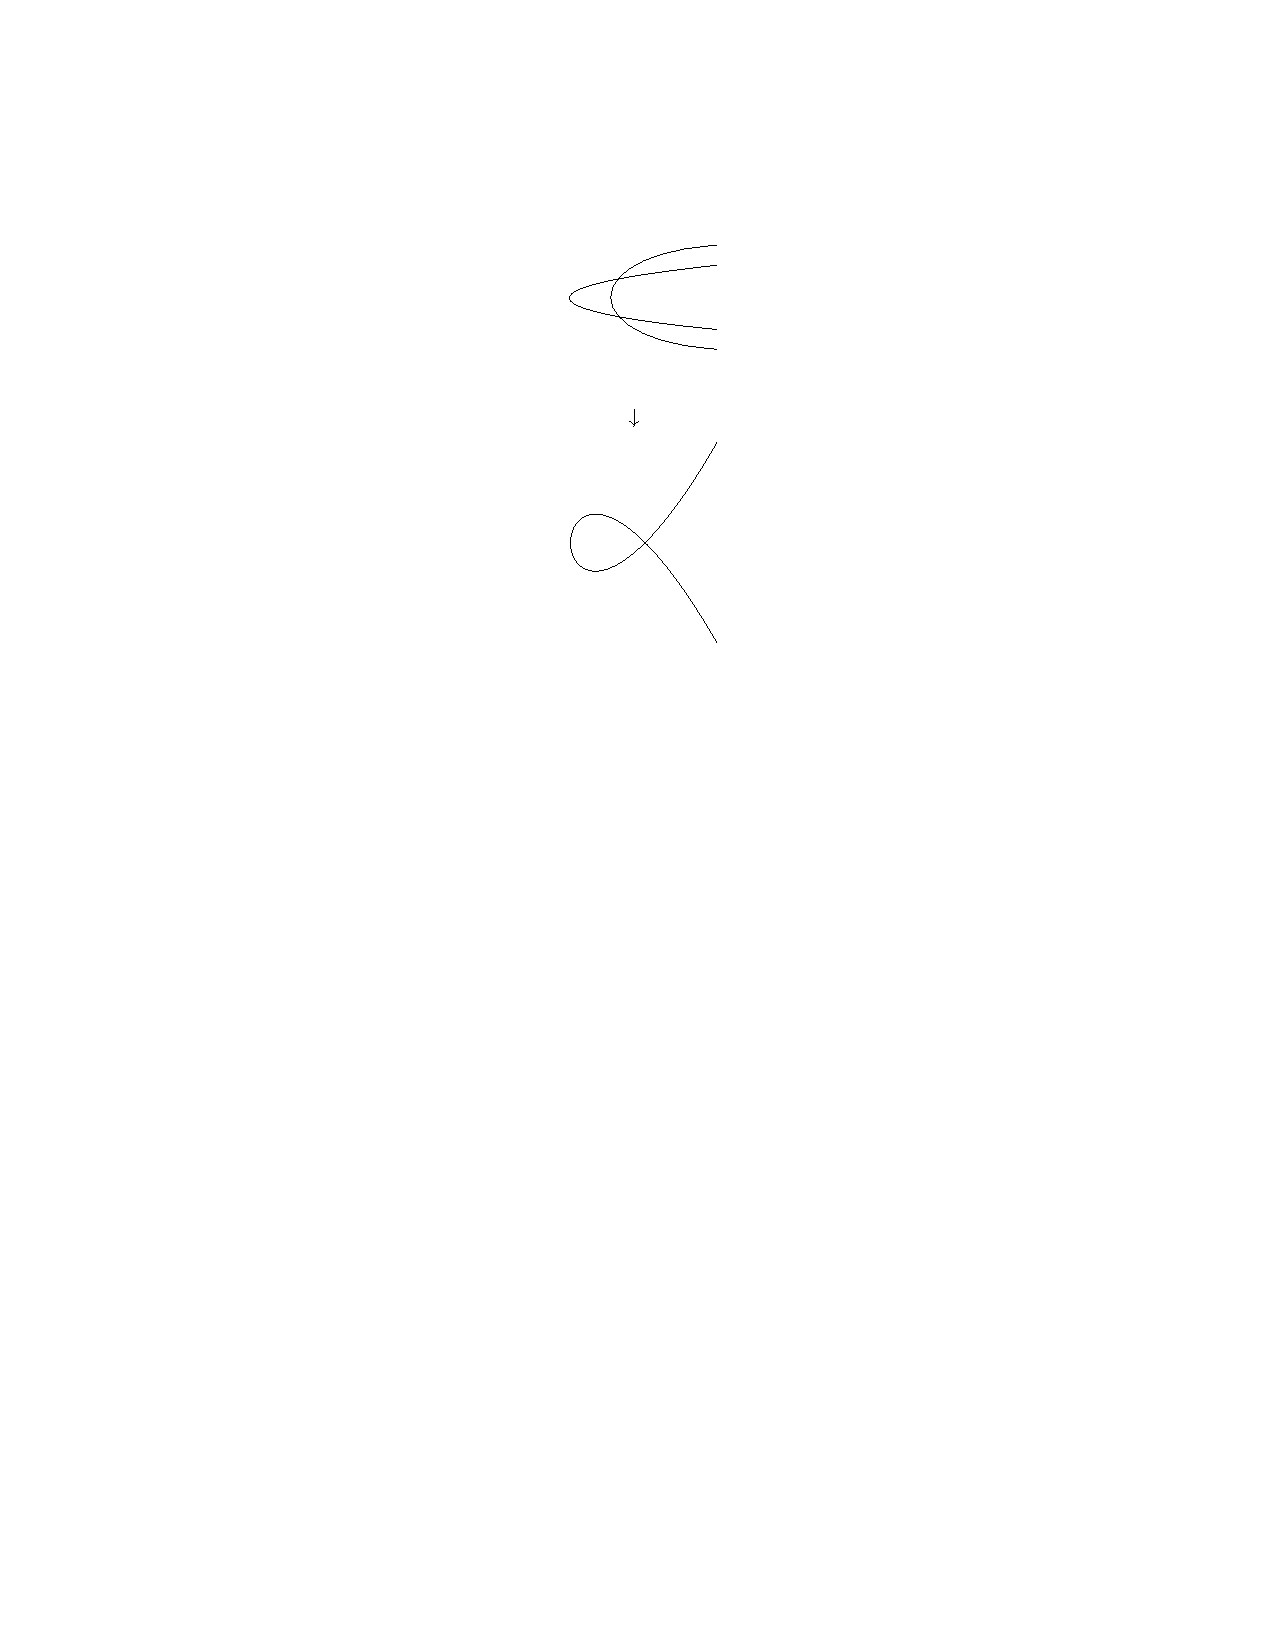
\includegraphics[width=0.4798\linewidth]{images/fig-2-1.pdf}
\caption{曲线 $V(y^2-x^3-x^2)$ 的二重覆盖。}\label{fig:2.1}
\end{figure}
光滑情形应当像一个投影：切向量可以提升，但提升未必唯一。平展情形则像把两条曲线映到一条曲线上；通过 $\varphi$ 选定上方的一点后，提升就是唯一的。一个有分歧且并非光滑的例子，是代数映射 $z\mapsto z^2$ 所给出的覆盖 $\mathbb A^1\to\mathbb A^1$。在分歧点，非零切向量不能提升，零切向量则可以有不唯一的提升。
\subsection{叠的例子}
\examnum{16}\begin{example}\label{ex:2.16}
设 $\mathcal F$ 是由函子
\Eq{2.44}{F:\mathcal S^{\mathrm{op}}\longrightarrow\Set}
关联得到的纤维群胚。则 $\mathcal F$ 是叠，当且仅当 $F$ 是平展拓扑中的集合层。若 $F=\Hom_S(-,X)$，$X\in\mathcal S$，则它是叠，这需要态射的平展下降。注意，模函子 $F_g$ 一般不是层，因此其关联群胚不是叠：曲线族的同构类未必能满足层的粘合要求。
\end{example}
\examnum{17}\begin{example}\label{ex:2.17}模群胚 $\mathcal M_g$ 是叠。\end{example}
\thmnum{proposition}{3}\begin{proposition}\label{pro:2.3}
设 $G/S$ 是一个平坦群概形，采用仿射、分离的情形，且 $G$ 作用于 $X$。则 $[X/G]$ 是叠。
\end{proposition}
\begin{proof}
对于对象下降条件，需要 $G$ 主丛，即 $G$ 挠子的平展下降。
对于态射下降条件，我们断言 $\operatorname{Iso}_B(f,f')$ 可由概形表示，其中对象为
\Eq{2.45}{\begin{tikzcd}E\arrow[r,"{f}"]\arrow[d]\&X\&E'\arrow[l,"{f'}"']\arrow[dll]\\B\end{tikzcd}.}
可以在使主丛平凡的平展局部计算，并用下降得到结论。因此暂设 $E=B\times G=E'$。选取截面 $\sigma:B\to E$ 和 $\sigma':B\to E'$，得到两个态射 $s=f\circ\sigma$、$s'=f'\circ\sigma':B\to X$。
\SourcePage{34}
主丛之间的等变同构由一个 $G$ 值参数描述；与 $f,f'$ 相容，要求 $s=g\cdot s'$。所以
\Eq{2.46}{\operatorname{Iso}_B(f,f')\simeq B\times_{X\times_SX}(G\times_SX),}
其中 $G\times_SX\to X\times_SX$ 把 $(g,x)$ 映为 $(g\cdot x,x)$。它位于纤维图
\Eq{2.47}{\begin{tikzcd}\operatorname{Iso}_B(f,f')\arrow[r]\arrow[d]\&G\times_SX\arrow[d,"{(g,x)\mapsto(gx,x)}"]\\B\arrow[r,"{(s,s')}"]\&X\times_SX\end{tikzcd}.}

\end{proof}
\begin{Note}{2.8}对概形本身，而不仅是其态射，进行平展下降，会导向代数空间的概念；这是 Artin 与 Knutson 的工作。\end{Note}
\examnum{18}\begin{example}\label{ex:2.18}
若 $\mathcal F,\mathcal G,\mathcal H$ 都是叠，且有态射 $\mathcal F\to\mathcal G$ 和 $\mathcal H\to\mathcal G$，则 $\mathcal F\times_{\mathcal G}\mathcal H$ 也是叠。
\end{example}
\subsection{可表态射}
某些叠之间的态射具有类似于概形的性质。
\thmnum{definition}{7}\begin{definition}\label{def:2.7}
叠态射 $f:\mathcal F\to\mathcal G$ 称为\Term{kebiaotaishi}{可表态射}，如果对任意概形 $B$ 及态射 $B\to\mathcal G$，纤维积 $B\times_{\mathcal G}\mathcal F$ 是一个概形的关联群胚。更一般且更合适的定义，允许它是代数空间。
\end{definition}
\examnum{19}\begin{example}\label{ex:2.19}
考虑 $X\to[X/G]$。使下图成为纤维图的 $E$ 是一个概形：
\Eq{2.48}{\begin{tikzcd}E\arrow[r]\arrow[d]\&X\arrow[d]\\B\arrow[r]\&{[X/G]}\end{tikzcd}.}
\end{example}
\examnum{20}\begin{example}\label{ex:2.20}
回忆，$\mathcal M_g$ 是亏格为 $g$ 的光滑曲线的模叠，而 $\mathcal C_g\to\mathcal M_g$ 还记住一个截面。对于 $B$ 上的曲线族 $C$，有纤维图
\Eq{2.49}{\begin{tikzcd}C\arrow[r]\arrow[d]\&\mathcal C_g\arrow[d]\\B\arrow[r]\&\mathcal M_g\end{tikzcd}.}
\end{example}
其思想是：对于在基变换下稳定的概形态射性质，它们与叠的思想相容，因此可以把这些性质移到叠的世界中。
\thmnum{definition}{8}\begin{definition}\label{def:2.8}
设 $\mathcal F\to\mathcal G$ 可表。对于在基变换下稳定的概形态射性质 $P$，\footnote{例如有限型、分离、平坦、仿射、固有等。}称该态射具有性质 $P$，如果对于每个概形 $B$ 及态射 $B\to\mathcal G$，$B\times_{\mathcal G}\mathcal F\to B$ 都具有该性质。
\end{definition}
\examnum{21}\begin{example}\label{ex:2.21}
若 $G/S$ 光滑，且 $G$ 作用于 $X$，则 $X\to[X/G]$ 光滑。
\end{example}
\SourcePage{35}
\subsection{Deligne–Mumford 叠的定义}
\thmnum{definition}{9}\begin{definition}\label{def:2.9}
叠 $\mathcal F$ 称为 \Term{delignemumforddie}{Deligne–Mumford 叠}，如果：
\begin{enumerate}
\item 对角态射 $\Delta_{\mathcal F}:\mathcal F\to\mathcal F\times_S\mathcal F$ 可表、拟紧且分离。\footnote{后两个条件有时会被放宽。}若 $\Delta_{\mathcal F}$ 还固有，则称 $\mathcal F$ 分离。
\item 存在平展满射 $\varphi:U\to\mathcal F$，其中 $U$ 是概形，称为平展图册。
\end{enumerate}
\end{definition}
\Lecture{9}{2019年9月26日}
下面作一些说明。
\begin{enumerate}
\item 首先讨论 $\Delta_{\mathcal X}$ 的可表性。
\thmnum{proposition}{4}\begin{proposition}\label{pro:2.4}
$\Delta_{\mathcal X}$ 可表，当且仅当每个从概形 $B$ 到 $\mathcal X$ 的态射都可表。
\end{proposition}
\begin{proof}
“$\Rightarrow$”：对于两个概形 $B,B'$，要证明图表中的 $B'\times_{\mathcal X}B$ 是概形：
\Eq{2.50}{\begin{tikzcd}B'\times_{\mathcal X}B\arrow[r]\arrow[d]\&B\arrow[d,"{f}"]\\B'\arrow[r,"{g}"]\&\mathcal X\end{tikzcd}.}
这由 $\Delta_{\mathcal X}$ 可表推出，因为有纤维图
\Eq{2.51}{\begin{tikzcd}B'\times_{\mathcal X}B\arrow[r]\arrow[d]\&\mathcal X\arrow[d,"{\Delta_{\mathcal X}}"]\\B'\times_SB\arrow[r,"{g\times f}"]\&\mathcal X\times_S\mathcal X\end{tikzcd}.}

\end{proof}
另一个方面是：若 $X,Y\in\Obj(\mathcal F(B))$，则 $\operatorname{Iso}_B(X,Y)$ 由概形表示。
\begin{proof}
$X,Y$ 对应于两个映射 $f,g:B\to\mathcal X$。同构函子由下面的纤维积表示：
\Eq{2.52}{\begin{tikzcd}B\times_{\mathcal X\times_S\mathcal X}\mathcal X\arrow[r]\arrow[d]\&\mathcal X\arrow[d,"{\Delta_{\mathcal X}}"]\\B\arrow[r,"{(f,g)}"]\&\mathcal X\times_S\mathcal X\end{tikzcd}.}
由可表性，它就是一个概形。
\end{proof}
\item $\Delta_{\mathcal X}$ 拟紧：我们不希望 $\operatorname{Iso}_B(X,Y)$ 过于失控。这个条件可以放宽，例如 Stacks Project 采用的定义就更一般。
\item $\Delta_{\mathcal X}$ 分离：若一个同构在一般点处为恒等，它就为恒等。
\item 什么时候 $\Delta_{\mathcal X}$ 固有？这应当与叠 $\mathcal X$ 的分离性有关。对于概形，通常要求 $X\to X\times_SX$ 是闭嵌入。
\SourcePage{36}
\item 图册提供了 Artin 环上的变形所需的通用变形空间。写 $\bar A=A/I$，其中 $I^n=0$。其想法是：在
\Eq{2.53}{\begin{tikzcd}\Spec\bar A\arrow[r]\arrow[d]\&U\arrow[d]\\\Spec A\arrow[r]\arrow[ur,dashed]\&\mathcal X\end{tikzcd}}
中得到相应的唯一提升。
\item 图册平展，使 $\Delta_{\mathcal F}$ 非分歧，即自同构在某种意义上是离散的。若只有光滑图册，则称为 Artin 叠，或代数叠。
\examnum{22}\begin{example}\label{ex:2.22}
对于平坦但未必平展的群概形 $G/S$，相应的 $BG=[\mathrm{pt}/G]$ 给出 Artin 叠的例子。
\end{example}
\end{enumerate}
\UnnumberedSubsection{叠的分离性}
\thmnum{lemma}{5}\begin{lemma}\label{lem:2.5}
设 $f:\mathcal F\to\mathcal G$ 是满足上述对角态射条件的叠之间的态射，则相对对角态射 $\Delta_{\mathcal F/\mathcal G}:\mathcal F\to\mathcal F\times_{\mathcal G}\mathcal F$ 可表。
\end{lemma}
\begin{proof}见文献 \cite{ref20}。\end{proof}
\UnnumberedSubsection{Artin 叠成为 Deligne–Mumford 叠的判别准则}
\thmnum{theorem}{6}\begin{theorem}\label{thm:2.6}
设 $\mathcal F$ 为 Noether 概形 $S$ 上的代数叠，具有一个在 $S$ 上有限型的光滑图册 $U\to\mathcal F$。则 $\mathcal F$ 是 Deligne–Mumford 叠，当且仅当 $\Delta_{\mathcal F}$ 非分歧。
\end{theorem}
\begin{proof}见文献 \cite{ref20}，或文献 \cite{ref9} 的定理 2.1。\end{proof}
\thmnum{corollary}{7}\begin{corollary}\label{cor:2.7}
设 $G/S$ 为作用于 Noether 概形 $X/S$ 的光滑仿射群概形，两者在 $S$ 上均有限型，且几何点的稳定子有限并约化。则：
\begin{enumerate}[label=(\roman*)]
\item $[X/G]$ 是 Deligne–Mumford 叠；若稳定子平凡，它是代数空间。
\item $[X/G]$ 分离，当且仅当作用态射固有。
\end{enumerate}
\end{corollary}
\begin{proof}
证明第一点。稳定子有限并约化意味着，对于任意对象
\Eq{2.54}{B\to[X/G]\quad\longleftrightarrow\quad\left(\begin{tikzcd}E\arrow[r]\arrow[d]\&X\\B\end{tikzcd}\right),}
$\operatorname{Iso}_B(E,E)\to B$ 非分歧。因此 $\Delta_{[X/G]}$ 非分歧，而 $X\to[X/G]$ 光滑，由\hyperref[thm:2.6]{上述定理}可知 $[X/G]$ 是 Deligne–Mumford 叠。
\end{proof}
\section{稳定曲线}
要得到曲线的完备模叠，即直观上的紧模叠，必须加入奇异曲线。Deligne 与 Mumford 的洞见是：加入结点就足够了。\footnote{结点的意思是，平展局部看起来像 $V(zw)\subset\mathbb A^2$。}
\SourcePage{37}
\Needspace{10\baselineskip}\thmnum{definition}{10}\begin{definition}\label{def:2.10}
概形 $S$ 上的一条 Deligne–Mumford 稳定曲线，是固有平坦态射 $\pi:C\to S$，满足：
\begin{enumerate}[label=(\roman*)]
\item 几何纤维 $C_s$ 约化、连通、一维，其奇点至多为结点；
\item 若 $E\subset C_s$ 是一个正规化为光滑有理曲线的不可约分支，$\nu:\widetilde E\to E$ 为正规化，则奇点在 $\widetilde E$ 中的原像至少有 $3$ 个。
\end{enumerate}
同时，不允许 $C_s$ 是亏格为 $0$ 或 $1$ 的光滑曲线。
\end{definition}
\begin{Note}{2.9}条件 (ii) 连同上述排除情形，等价于 $\Aut(C_s)$ 有限。\end{Note}
注意，亏格为 $g=h^1(C_s,\OO_{C_s})$。这些对象立即构成亏格为 $g$ 的稳定曲线群胚 $\overline{\mathcal M}_g$；目前，它是 $\ZZ$ 上的一个叠。
\subsection{稳定曲线模叠是 Deligne–Mumford 叠}
回忆，对于稳定曲线，$\pi:C\to S$ 是平展局部完全交态射，因此具有相对对偶化可逆层 $\omega_{C/S}$。在几何纤维上，可显式考虑正规化
\Eq{2.55}{\nu:C_s'\longrightarrow C_s,\qquad x_i,y_i\longmapsto\text{第 }i\text{ 个结点}.}
于是
\Eq{2.56}{\nu^*\omega_{C_s}=\omega_{C_s'}(x_1+\cdots+x_r+y_1+\cdots+y_r).}
若 $\alpha\in\omega_{C_s}(U)$，其中 $U$ 为第 $i$ 个结点的邻域，则 $\nu^*\alpha$ 是一个有理一形式，且
\Eq{2.57}{\operatorname{Res}_{x_i}(\nu^*\alpha)+\operatorname{Res}_{y_i}(\nu^*\alpha)=0.}
现在用 $\omega_{C/S}^{\otimes n}$ 将 $C/S$ 嵌入某个 $\PP_S^N$。
\thmnum{theorem}{8}\begin{theorem}\label{thm:2.8}
若 $g\ge2$，则当 $n\ge3$ 时，$\omega_{C/S}^{\otimes n}$ 相对甚丰。此外，$\pi_*(\omega_{C/S}^{\otimes n})$ 局部自由，秩为 $(2n-1)(g-1)$。
\end{theorem}
\Lecture{10}{2019年10月1日}
\begin{proof}
这里只给出证明概要。对于光滑曲线，当 $g\ge3$ 时，$\omega_{C/S}^{\otimes n}$ 在 $n\ge2$ 时就相对甚丰；亏格 $2$ 时采用 $n\ge3$。先考虑 $S=\Spec k$。由 Riemann–Roch 定理与 Serre 对偶性，
\Eq{2.58}{h^0(C,\omega_C^{\otimes n})=h^1(C,\omega_C^{\otimes n})+\deg(\omega_C^{\otimes n})+1-g,}
\Eq{2.59}{=h^0\bigl(C,(\omega_C^{\otimes n})^{-1}\otimes\omega_C\bigr)+n(2g-2)+1-g.}
对于光滑曲线，$(\omega_C^{\otimes n})^{-1}\otimes\omega_C=\omega_C^{1-n}$，其次数为 $(1-n)(2g-2)<0$，所以 $h^0(C,\omega_C^{1-n})=0$，得到
\Eq{2.60}{h^0(C,\omega_C^{\otimes n})=(2n-1)(g-1).}
在所需的 $n$ 范围内，对 $\omega_C^{\otimes n}(-p_1-p_2)$ 使用同样的对偶论证，仍有一阶上同调消失。因此能分离点和切向量，这是甚丰性的判别条件。
若 $C$ 是结点曲线，取正规化 $\nu:C'\to C$，其中 $C'$ 光滑。则
\Eq{2.61}{C_{\mathrm{sing}}=\{z_1,\ldots,z_r\},\qquad\nu^{-1}(z_i)=\{x_i,y_i\}.}
\SourcePage{38}
对于 $\alpha\in H^0(U,\omega_C)$，$\nu^*\alpha$ 是 $\omega_{C'}=\Omega_{C'}^1$ 的有理截面，在 $x_i,y_i$ 处至多有一阶极点，并满足两点留数之和为零。因此
\Eq{2.62}{\nu^*\omega_C=\Omega_{C'}^1\left(\sum_i x_i+\sum_i y_i\right).}
无论如何，这说明当 $n\ge3$ 时，$\omega_C^{\otimes n}$ 甚丰。最不利的情形，是 $C$ 有一个带 $3$ 个特殊点的有理不可约分支 $D$；此时
\Eq{2.63}{\nu^*\omega_C|_D\simeq\OO_{\PP^1}(1).}
最后使用上同调与基变换。
\end{proof}
\thmnum{corollary}{9}\begin{corollary}\label{cor:2.9}
每条亏格为 $g$ 的稳定曲线 $C$，都可通过 $n$-典范嵌入进入 $\PP^N$，其中 $N=(2n-1)(g-1)-1$、$n\ge3$，其 Hilbert 多项式为
\Eq{2.64}{P_{g,n}(t)=(2nt-1)(g-1).}
\end{corollary}
\thmnum{definition}{11}\begin{definition}\label{def:2.11}
$H_{g,n}\subset\operatorname{Hilb}_{\PP^N}^{P_{g,n}}$ 由通过 $n$-典范嵌入给出的稳定结点曲线组成。
\end{definition}
这里的典范嵌入条件给出相应的局部闭子概形，而结点条件为开条件：结点至多被光滑化。
\begin{Note}{2.10}
\begin{enumerate}[label=(\alph*)]
\item 给出态射 $S\to H_{g,n}$，等价于给出亏格为 $g$ 的稳定曲线 $\pi:C\to S$，以及同构 $\PP(\pi_*(\omega_{C/S}^{\otimes n}))\xrightarrow{\sim}S\times\PP^N$。
\item $\mathrm{PGL}(N+1)$ 通过它在 $\PP^N$ 上的作用，作用于 $H_{g,n}$。
\end{enumerate}
\end{Note}
\thmnum{theorem}{10}\begin{theorem}\label{thm:2.10}
$\overline{\mathcal M}_g\simeq[H_{g,n}/\mathrm{PGL}(N+1)]$。
\end{theorem}
\begin{proof}
我们将定义函子
\Eq{2.65}{p:\overline{\mathcal M}_g\longrightarrow[H_{g,n}/\mathrm{PGL}(N+1)].}
在对象上，
\Eq{2.66}{(C\xrightarrow\pi B)\longmapsto(E\longrightarrow B),}
其中 $E$ 是与 $\PP(\pi_*\omega_{C/B}^{\otimes n})=P/B$ 关联的 $\mathrm{PGL}(N+1)$ 主丛。还需要一个 $\mathrm{PGL}(N+1)$ 等变态射 $E\to H_{g,n}$。考虑
\Eq{2.67}{\begin{tikzcd}C\times_BE\arrow[r]\arrow[d,"{\widetilde\pi}"']\&C\arrow[d,"{\pi}"]\\E\arrow[r]\&B\end{tikzcd}.}
现在
\Eq{2.68}{E\times_BP=\PP\bigl(\widetilde\pi_*(\omega_{C\times_BE/E}^{\otimes n})\bigr)}
是平凡的，因为在标架主丛上，拉回的射影丛具有典范的平凡化。在态射上，考虑
\Eq{2.69}{\begin{tikzcd}C'\arrow[r]\arrow[d,"{\pi'}"']\&C\arrow[d,"{\pi}"]\\B'\arrow[r,"{\varphi}"]\&B\end{tikzcd}.}
\SourcePage{39}
它给出
\Eq{2.70}{\pi'_*(\omega_{C'/B'}^{\otimes n})\simeq\varphi^*\pi_*(\omega_{C/B}^{\otimes n}),}
从而导出笛卡尔方块
\Eq{2.71}{\begin{tikzcd}E'\arrow[r]\arrow[d]\&E\arrow[d]\\B'\arrow[r]\&B\end{tikzcd}.}
\begin{Note}{2.11}
$p$ 完全忠实且本质满。这些性质都有几何含义。忠实性表示，$C$ 上一个非平凡自同构，会在 $\PP(H^0(\omega_C^{\otimes n}))$ 上诱导非平凡自同构。满性表示，若 $\Phi\in\mathrm{PGL}(N+1)$ 满足 $\Phi(C)=C$，那么 $\Phi$ 来自 $C$ 的自同构；这里也用到 $n$-典范嵌入不包含在真线性子空间中。
本质满性表示如下事实。设
\Eq{2.72}{\left(\begin{tikzcd}E\arrow[r]\arrow[d]\&H_{g,n}\\B\end{tikzcd}\right)\in\Obj[H_{g,n}/\mathrm{PGL}(N+1)].}
则有 $\pi_E:C_E\to E$，以及同构
\Eq{2.73}{\PP\bigl(\pi_{E*}(\omega_{C_E/E}^{\otimes n})\bigr)\simeq E\times\PP^N.}
这些数据下降为
\Eq{2.74}{B=E/\mathrm{PGL}(N+1),\qquad C=C_E/\mathrm{PGL}(N+1).}
\end{Note}

\end{proof}
\thmnum{corollary}{11}\begin{corollary}\label{cor:2.11}
$\overline{\mathcal M}_g$ 是 $S$ 上有限型的分离 Deligne–Mumford 叠，例如可以取 $S=\Spec\ZZ$ 或 $S=\Spec k$。
\end{corollary}
\begin{proof}
使用文献 \cite{ref8} 中的判别准则，并通过验证 $\operatorname{Iso}_B(C',C)\to B$ 的有限性来检查分离性。细节见文献 \cite{ref8}。
\end{proof}
\subsection{进一步的性质}
\thmnum{proposition}{12}\begin{proposition}\label{pro:2.12}
$\overline{\mathcal M}_g$ 是固有的，基可以是 $\Spec\ZZ$ 或 $\Spec k$。
\end{proposition}
\begin{custom}{插叙 1：叠及其态射的性质}\hypertarget{digression:2.1}{}
对于在光滑拓扑中局部的性质，在 Deligne–Mumford 情形下则用平展拓扑，例如平坦、光滑、局部 Noether、正规等，可以在光滑图册上检查。非分歧性可在适用的平展图册上检查。固有性则不属于这种形式的性质。
\end{custom}
\thmnum{definition}{12}\begin{definition}\label{def:2.12}
叠态射 $f:\mathcal X\to\mathcal Y$ 称为\Term{guyou}{固有}，如果它分离、有限型且普遍闭；最后一个条件使用 $|\mathcal X|$ 与 $|\mathcal Y|$ 上的 Zariski 拓扑。\footnote{该拓扑由可表开嵌入 $U\to\mathcal X$，以及相应的 $U\to\mathcal Y$ 生成。}
\end{definition}
我们不会直接使用这个定义，而是通常采用固有性的赋值判别准则。
\SourcePage{40}
先陈述概形的情形。设 $R$ 为离散赋值环，$K$ 是其分式域，考虑
\Eq{2.75}{\begin{tikzcd}\Spec K\arrow[r]\arrow[d]\&X\arrow[d]\\\Spec R\arrow[r]\arrow[ur,dashed,"{?}"']\&Y\end{tikzcd}.}
此时，这一箭头的唯一性对应于分离性；其存在性给出固有性的判别。
对于叠，允许先取有限扩张 $K'/K$，再令 $R'$ 为 $R$ 在 $K'$ 中的整闭包，然后询问下面的提升是否存在，以及是否唯一：
\Eq{2.76}{\begin{tikzcd}\Spec K'\arrow[r]\arrow[d]\&\Spec K\arrow[r]\arrow[d]\&X\arrow[d]\\\Spec R'\arrow[r]\arrow[urr,dashed,"{?}"']\&\Spec R\arrow[r]\&Y\end{tikzcd}.}
在模理论中，这称为\Term{wendingyuehua}{稳定约化}。
\Lecture{11}{2019年10月3日}
考虑 $\overline{\mathcal M}_g/\Spec\ZZ$，其中 $g\ge2$。事实是：
\thmnum{theorem}{13}\begin{theorem}\label{thm:2.13}$\overline{\mathcal M}_g$ 固有。\end{theorem}
由上述赋值判别准则，只需证明：
\thmnum{theorem}{14}\begin{theorem}\label{thm:2.14}
设 $R$ 为离散赋值环，$B=\Spec R$，$K$ 为 $R$ 的分式域。给定稳定曲线 $f:X_K\to\Spec K$，存在有限扩张 $K'/K$，以及在固定基变换和一般纤维同构后唯一的稳定曲线 $X'\to B'$。这里 $B'=\Spec R'$，$R'$ 是 $R$ 在 $K'$ 中的整闭包，且
\Eq{2.77}{X_{K'}\simeq X_K\times_{\Spec K}\Spec K',}
位于图表
\Eq{2.78}{\begin{tikzcd}X'\arrow[d]\&X_{K'}\arrow[l,hook']\arrow[r]\arrow[d]\&X_K\arrow[d]\\B'\&\Spec K'\arrow[l,hook']\arrow[r]\&\Spec K\end{tikzcd}}
中。
\end{theorem}
\begin{proof}
在特征零情形下，先利用射影性，将其任意延拓为一个约化概形：
\Eq{2.79}{\begin{tikzcd}X_K\arrow[r]\arrow[d]\&\overline X\arrow[r,hook]\arrow[d]\&\PP_R^N\\\Spec K\arrow[r]\&B=\Spec R\end{tikzcd}.}
注意，$\overline X$ 是一个曲面。现在消解 $X\to\overline X$；可以通过反复吹起显式完成，使特殊纤维的支撑呈正规交叉。取 $0$ 处纤维，得到类似结点曲线的 $X_0$，但它未必约化。
$R$ 有一致化参数 $t\in R$，其极大理想为 $\mathfrak m=(t)$。随后作基变换 $t\mapsto t^l$，\footnote{这里使用特征零。若特征 $p$ 整除 $l$，情形就会非常棘手。}$l$ 是 $X_0$ 各分支重数的最小公倍数；再正规化并进行必要的消解，得到 $\widetilde X'\to B'=\Spec R'$，其特殊纤维是约化结点曲线。不过它未必稳定，最后收缩不稳定的有理分支即可。
\end{proof}
\SourcePage{41}
\thmnum{theorem}{15}\begin{theorem}\label{thm:2.15}
$\overline{\mathcal M}_g$ 光滑且连通，其边界 $\overline{\mathcal M}_g\setminus\mathcal M_g$ 是正规交叉除子，具有 $\lfloor g/2\rfloor+1$ 个不可约分支。这里 $\mathcal M_g$ 参数化光滑曲线。
\end{theorem}
\begin{proof}
光滑性可以在光滑图册 $H_{g,n}\twoheadrightarrow\overline{\mathcal M}_g$ 上检查，而这一检查实际上就是变形理论。
对于连通性，定义 Hurwitz 空间
\Eq{2.80}{\operatorname{Hur}_{k,b}=\left\{C\to\PP^1\ \middle|\ \begin{array}{l}\text{只有简单分歧，次数为 }k,\\\text{分歧点数目为 }b,\\g(C)=b/2-k+1\end{array}\right\}.}
Hurwitz 证明，$\operatorname{Hur}_{k,b}$ 总是连通的。当 $k>g+1$ 时，有满射 $\operatorname{Hur}_{k,b}\twoheadrightarrow\mathcal M_g$，所以 $\mathcal M_g$ 连通，从而它的稳定紧化也连通。
\end{proof}
还有以下变体：
\begin{enumerate}[label=(\alph*)]
\item $\overline{\mathcal M}_{g,k}$ 由带 $k$ 个标记点的亏格 $g$ 稳定曲线组成。这时，自同构有限的条件变成
\Eq{2.81}{\#\Aut(C,\symbfit{x})<\infty,\qquad\symbfit{x}=(x_1,\ldots,x_k).}
此时必须有 $2g-2+k>0$，所以以下列表中的前三种亏格零情形和未标记的亏格一情形不允许：
\Eq{2.82}{\underbrace{\overline{\mathcal M}_{0,0},\ \overline{\mathcal M}_{0,1},\ \overline{\mathcal M}_{0,2}}_{\text{不允许}},\quad\overline{\mathcal M}_{0,3},\ \overline{\mathcal M}_{0,4},\ \overline{\mathcal M}_{0,5},\ldots,}
\Eq{2.83}{\underbrace{\overline{\mathcal M}_{1,0}}_{\text{不允许}},\quad\overline{\mathcal M}_{1,1},\ldots,}
\Eq{2.84}{\overline{\mathcal M}_{2,0},\ldots.}
\item 也可以考虑预稳定曲线，即去掉稳定性条件。幸运的是，Stacks Project 在这里提供了帮助，其中的处理具有更大的一般性。例如，允许同构函子由代数空间表示，这在很一般的情形下成立。这样得到的是一个 Artin 叠。
\end{enumerate}

\chapter{Gromov–Witten 理论与虚技术}
\SourcePage{42}
\section{稳定映射}
设 $X$ 为 $\CC$ 上（或其他特征零域上）的概形。
\thmnum{definition}{1}\begin{definition}\label{def:3.1}
定义\Term{wendingyingshe}{稳定映射}模叠的对象为
\Eq{3.1}{\overline{\mathcal M}_{g,k}(X)(B)=\left\{\left(\begin{tikzcd}C\arrow[r,"{f}"]\arrow[d,"{\pi}"']\&X\\B\arrow[u,bend left,"{\symbfit{x}}"]\end{tikzcd}\right)\ \middle|\ \begin{array}{l}(C,\symbfit{x})\in\widetilde{\mathcal M}_{g,k}(B),\\\text{对所有几何点 }s\to B,\\\#\Aut(C_s,\symbfit{x}_s,f_s)<\infty\end{array}\right\},}
其中 $\widetilde{\mathcal M}_{g,k}$ 是带标记点的结点曲线叠，且
\Eq{3.2}{\Aut(C_s,\symbfit{x}_s,f_s)=\{\,\varphi\in\Aut(C_s)\mid\varphi(x_i)=x_i\text{ 对每个 }i,\ f_s\circ\varphi=f_s\,\}.}
\end{definition}
当 $s=\Spec\CC$ 时，$f_s$ 的类为 $f_*[C]\in H_2(X,\ZZ)$，也可以在 $H_2(X,\QQ)$ 或 $A_1(X)$ 中考虑，其中 $[C]\in H_2(C,\ZZ)$。固定 $\beta\in H_2(X,\ZZ)$，即“次数”，得到开子叠
\Eq{3.3}{\overline{\mathcal M}_{g,k}(X,\beta)\subset\overline{\mathcal M}_{g,k}(X).}
现在解释这一定义。设 $f:(C,\symbfit{x})\to X/\Spec\CC$。对于每个不可约分支 $C'\subset C$，有对应的映射 $f:C'\to X$。只有两种可能：它要么是常值，要么在其像上有限。如果它有限，则已经有 $\#\Aut(C',f)<\infty$。所以真正有意思的，是被收缩的分支，也就是 $f$ 为常值的部分。
如果一条光滑亏格一曲线整体映为一点，并且没有特殊点，就必须排除这一情形，因为它的自同构群无限。一般的稳定性条件是：每个被收缩的有理分支至少有三个特殊点，每个被收缩的亏格一分支至少有一个特殊点；更高亏格的分支自身已有有限自同构群。注意，一个结点在正规化上对应两个特殊点。对于 $\PP^2$ 中次数 $d=3$ 的曲线，图 \ref{fig:3.1} 展示了嵌入曲线退化为 $y^2-x^3=0$ 一类尖点曲线的情形。
\UnnumberedSubsection{动机}
对于 $\PP^n$，其中 $n\ge3$，固定算术亏格的嵌入曲线空间可能高度奇异。但从稳定映射的角度看，至少在亏格零情形下：
\thmnum{theorem}{1}\begin{theorem}\label{thm:3.1}$\overline{\mathcal M}_{0,k}(\PP^n)$ 是光滑的。\end{theorem}
\begin{proof}
先考虑预稳定结点曲线叠 $\widetilde{\mathcal M}_{0,k}$。它是光滑的，因此只需证明遗忘映射
$\overline{\mathcal M}_{0,k}(\PP^n)\to\widetilde{\mathcal M}_{0,k}$，即 $(C,\symbfit{x},f)\mapsto(C,\symbfit{x})$，是叠之间的光滑态射。
\begin{figure}[H]\SourcePage{43}\centering
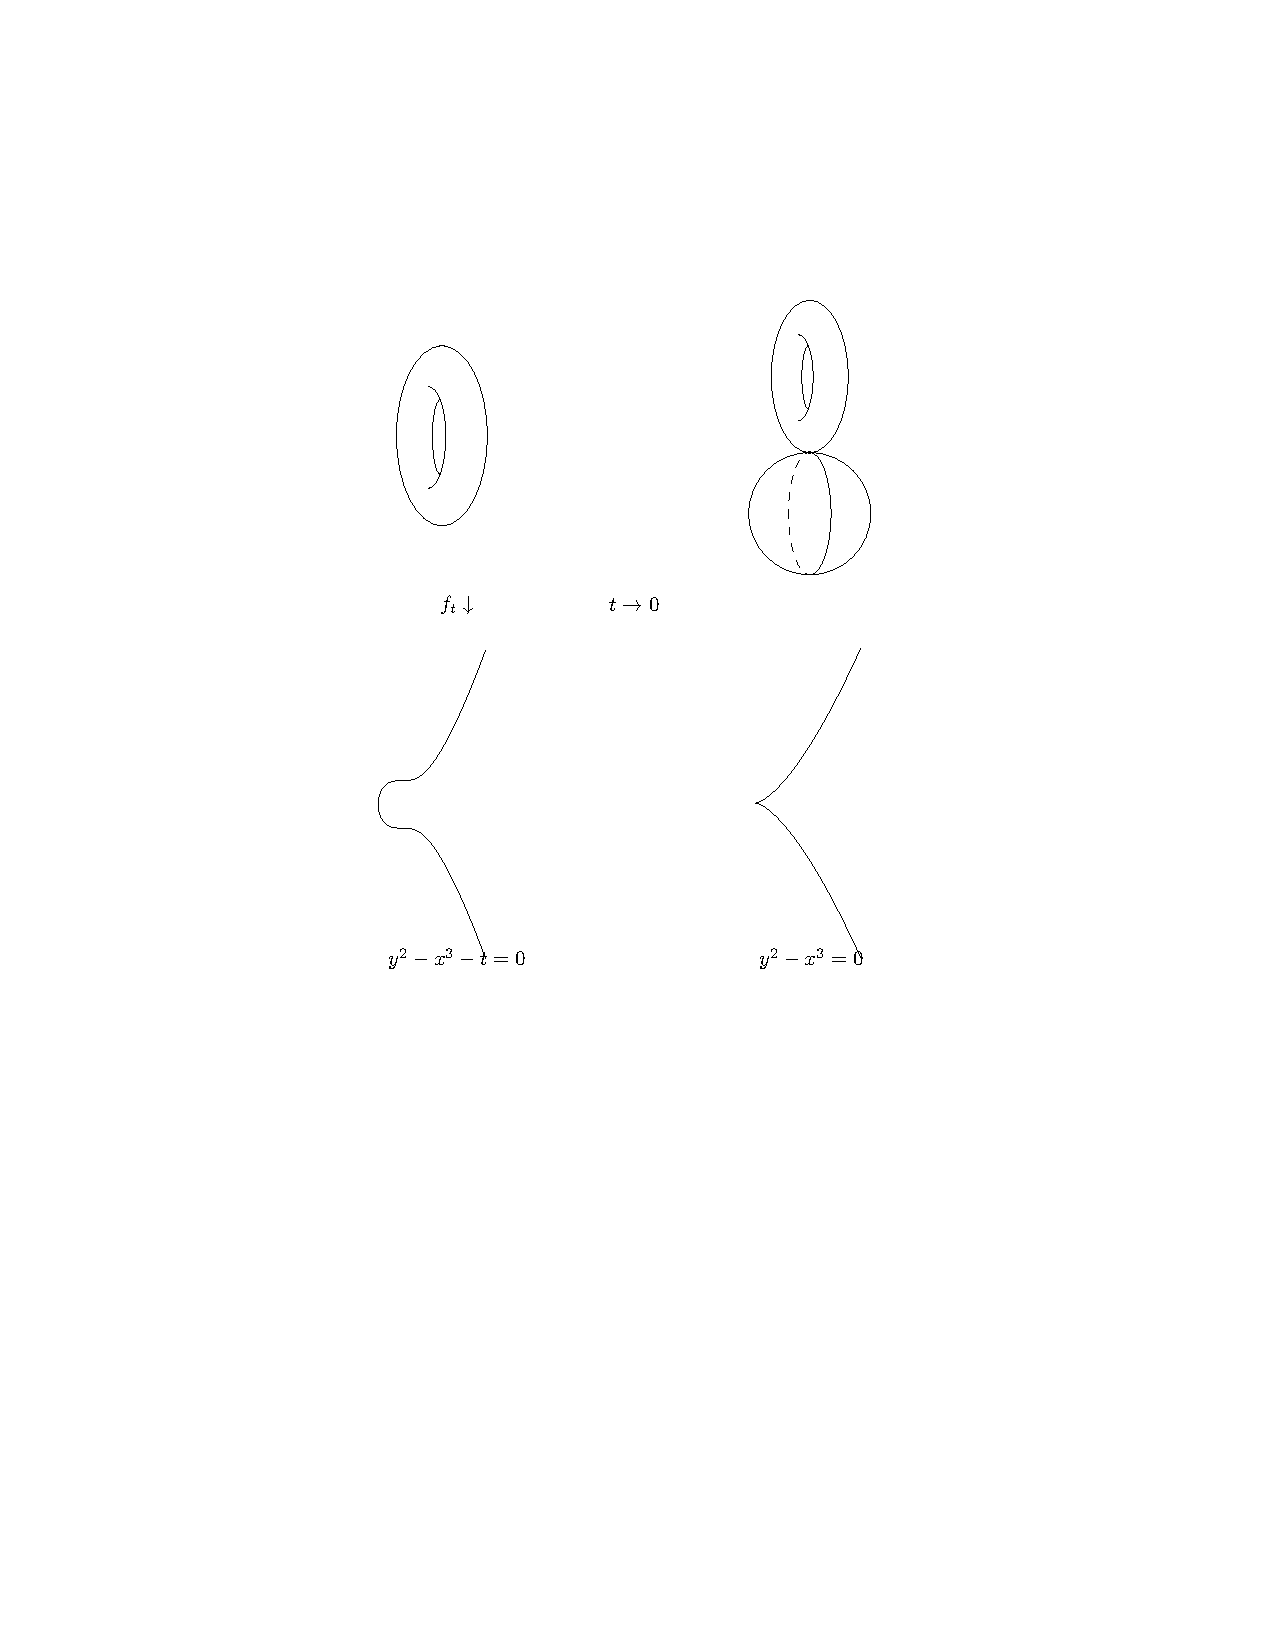
\includegraphics[width=0.6490\linewidth]{images/fig-3-1.pdf}
\caption{到 $\PP^2$ 的稳定映射族 $f_t$。当 $t\to0$ 时，亏格一的部分被收缩，像曲线因而出现尖点。}\label{fig:3.1}
\end{figure}
这归结为检查如下事项。对于 $\bar A=A/I$，其中 $I^2=0$，考虑
\Eq{3.4}{\begin{tikzcd}\Spec\bar A\arrow[r]\arrow[d]\&\overline{\mathcal M}_{0,k}(\PP^n)\arrow[d]\\\Spec A\arrow[r]\arrow[ur,dashed]\&\widetilde{\mathcal M}_{0,k}\end{tikzcd}.}
\SourcePage{44}
我们希望找到虚线箭头。换句话说，要找到
\Eq{3.5}{\begin{tikzcd}[row sep=2.3em,column sep=3em]\&\&X\\\bar C\arrow[rru,bend left=18,"{\bar f}"]\arrow[r,hook]\arrow[d]\&C\arrow[ur,dashed,"{\exists f?}"']\arrow[d]\\\Spec\bar A\arrow[r]\&\Spec A\end{tikzcd}}
中的 $f$：给定 $\bar f$，希望将其延拓。障碍类位于 $H^1(\bar C,\bar f^*\Theta_X)$ 中。在这里，$\bar f^*\Theta_{\PP^n}$ 在每个不可约分支 $\bar C'\subset\bar C$ 上整体生成，故有
\Eq{3.6}{0\longrightarrow K\longrightarrow\OO_{\bar C'}^{\oplus l}\longrightarrow\bar f^*\Theta_{\PP^n}|_{\bar C'}\longrightarrow0.}
在 $g=0$ 时，
\Eq{3.7}{0=H^1(\OO_{\bar C'})^{\oplus l}\longrightarrow H^1(\bar f^*\Theta_{\PP^n}|_{\bar C'})\longrightarrow H^2(K)=0.}

\end{proof}
\Lecture{12}{2019年10月8日}
\thmnum{theorem}{2}\begin{theorem}\label{thm:3.2}
若靶空间 $X$ 是射影概形，则 $\overline{\mathcal M}_{g,k}(X,\beta)$ 是固有、分离的 Deligne–Mumford 叠。
\end{theorem}
\begin{proof}
记 $\mathfrak m_{g,k}$ 为带 $k$ 个标记点的结点曲线的 Artin 叠。如果给定图表
\Eq{3.8}{\begin{tikzcd}C\arrow[r]\arrow[d]\&X\\T\arrow[u,bend left,"{\symbfit{x}}"]\end{tikzcd},}
这与下面的数据相同：
\Eq{3.9}{\begin{tikzcd}C\arrow[r]\arrow[d,"{\pi}"']\&X\times T\arrow[r]\arrow[d,"{\pr_2}"]\&X\arrow[d]\\T\arrow[r,equal]\arrow[u,bend left,"{\symbfit{x}}"]\&T\arrow[r]\&\mathrm{pt}\end{tikzcd}.}
它实际上是一个 $T$ 上的态射。无标记时，有万有曲线
\Eq{3.10}{\mathcal C_g\simeq\mathfrak m_{g,1}\longrightarrow\mathfrak m_g.}
因此，适当的带标记版本中，稳定映射叠嵌入相对 Hom 叠；无标记时记作
\Eq{3.11}{\overline{\mathcal M}_g(X)\hookrightarrow\Hom_{\mathfrak m_g}(\mathcal C_g,\mathfrak m_g\times X).}
右侧是一个局部有限型的 Artin 叠。由于稳定性为开条件，我们希望证明：
\thmnum{lemma}{3}\begin{lemma}\label{lem:3.3}稳定映射构成上述 Hom 叠的开子叠。\end{lemma}
\SourcePage{45}
\begin{figure}[H]\centering
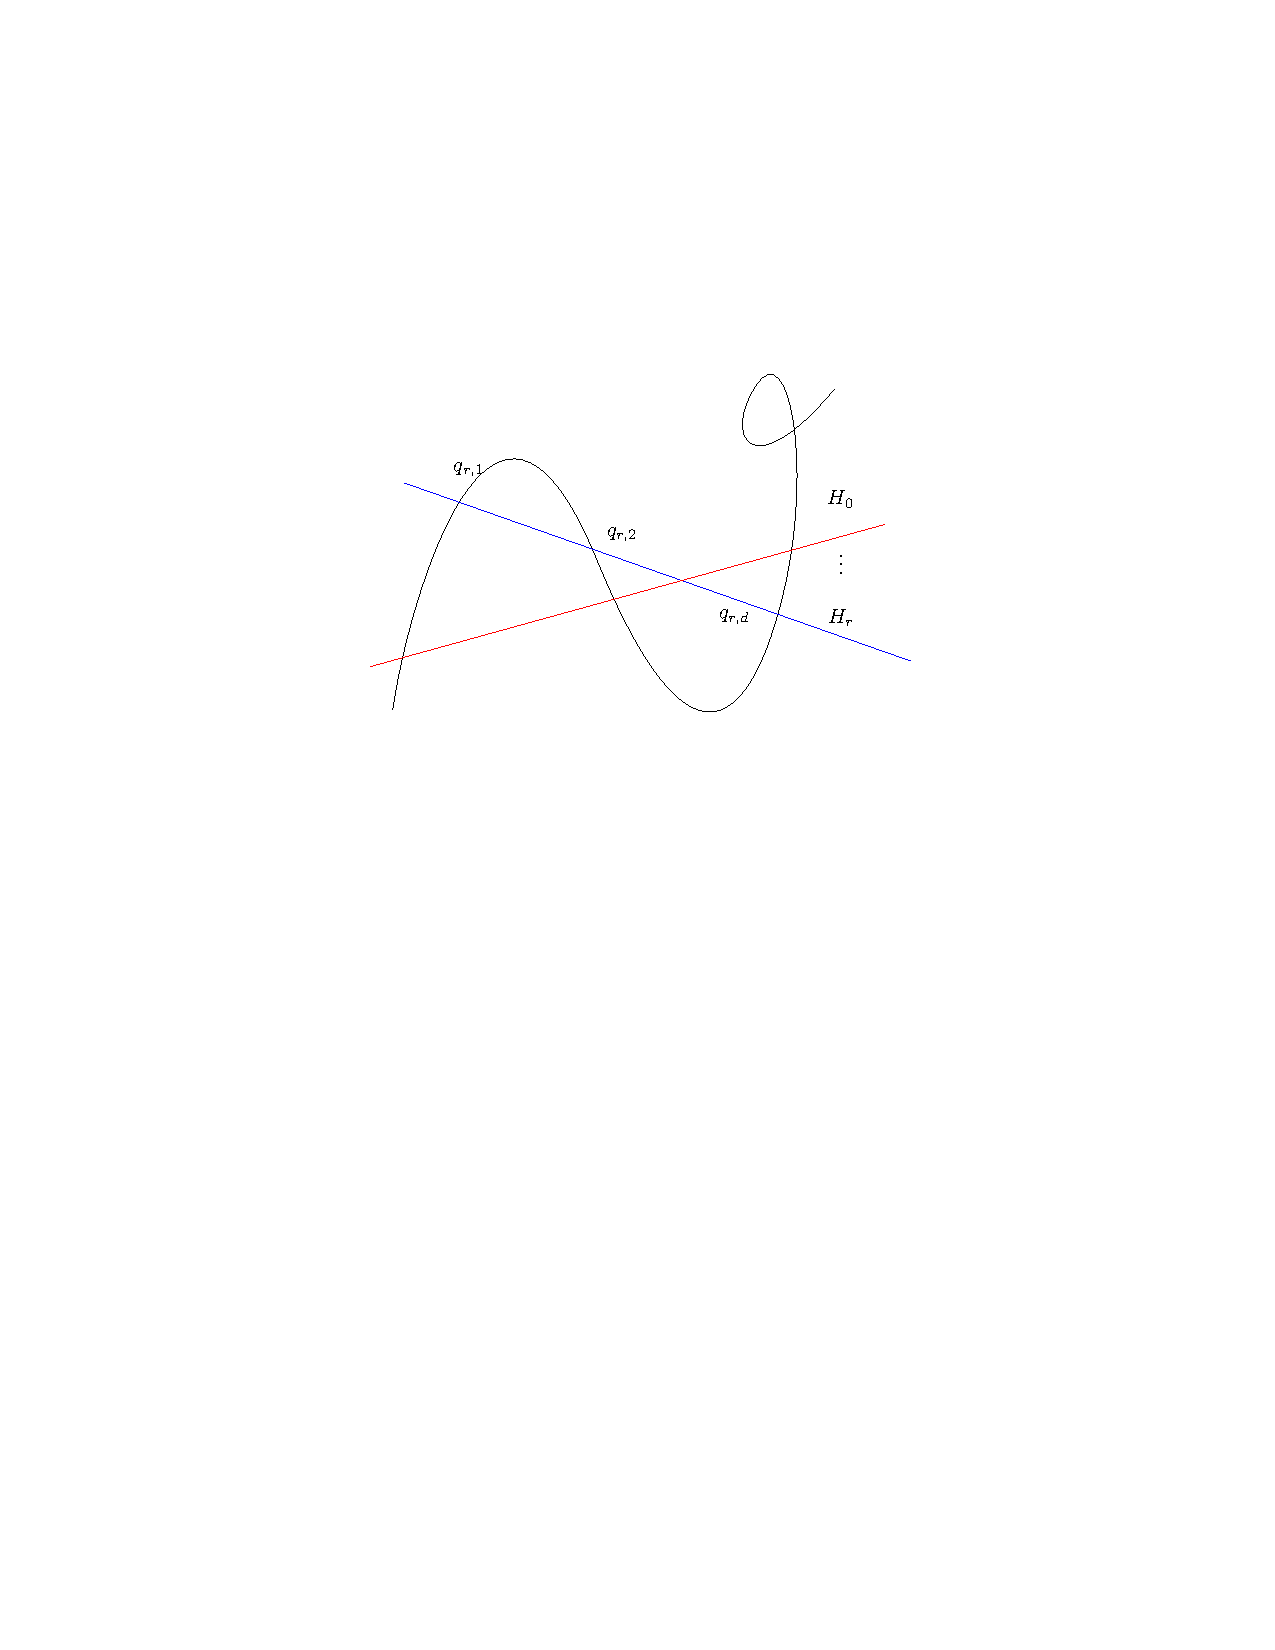
\includegraphics[width=0.6944\linewidth]{images/fig-3-2.pdf}
\caption{$\PP^r$ 中的 $r+1$ 个超平面与 $C_s$ 横截相交。}\label{fig:3.2}
\end{figure}
一旦固定 $\beta\in H_2(X,\ZZ)$，稳定映射只有有限多个“组合类型”。\footnote{这里指不可约分支的相交方式、各分支的亏格，以及每个分支的类 $\beta_i$，其中 $\beta=\sum_i\beta_i$。}这说明 $\overline{\mathcal M}_{g,k}(X,\beta)$ 拟紧。
更困难的部分是稳定约化，它给出分离性与固有性。Fulton 与 Pandharipande 的想法是：若 $X\subset\PP^r$，则有闭嵌入 $\overline{\mathcal M}(X,\beta)\hookrightarrow\overline{\mathcal M}(\PP^r,d)$，所以不妨取 $X=\PP^r$。关键在于
$L=\omega_{C/T}(\symbfit{x})\otimes f^*\OO_{\PP^r}(3)$ 对 $C/T$ 相对丰。因此，存在只依赖于 $g,k,d$ 的整数 $l$，使 $L^{\otimes l}$ 相对甚丰。
\end{proof}
考虑图 \ref{fig:3.2}。这些超平面 $H_i=(t_i=0)$，其中 $t_i\in\Gamma(\PP^r,\OO(1))$，在 $C$ 上给出额外标记点。于是，$\overline{\mathcal M}(\PP^r,d)$ 局部同构于刚化空间 $R$，其对象为
\Eq{3.12}{C\xrightarrow\pi T,\qquad\symbfit{q}=(q_{ij}),}
\SourcePage{46}
并满足一系列条件。定义
\Eq{3.13}{H_i=\OO_C(q_{i,1}+\cdots+q_{i,d}).}
对每个 $i$，要求
\Eq{3.14}{\pi^*\pi_*(H_i^{-1}\otimes H_0)\longrightarrow H_i^{-1}\otimes H_0}
为同构，并要求对所有 $i,j$ 都有 $H_i\simeq H_j$。还要给出 $\lambda_0,\ldots,\lambda_r:T\to\mathbb G_m$，用来调整 $H_i$ 的典范截面 $s_i$ 的尺度。
现在的想法，是在刚化后的层面进行稳定约化。
\section{超曲面的亏格零 Gromov–Witten 不变量}
设 $X\subset\PP^{n+1}$ 是次数为 $l$ 的超曲面，$X=Z(F)$。则 $\overline{\mathcal M}_0(X,d)\subset\overline{\mathcal M}_0(\PP^{n+1},d)$ 是一个向量丛截面的零点集。考虑万有图表
\Eq{3.15}{\begin{tikzcd}\mathcal C_0(\PP^{n+1})\arrow[r,"{f}"]\arrow[d,"{\pi}"']\&\PP^{n+1}\\\overline{\mathcal M}_0(\PP^{n+1})\end{tikzcd}.}
在几何纤维上，$f^*\OO(l)$ 在每个不可约分支上的次数都非负。$g=0$ 蕴含 $H^1(f_s^*\OO(l))=0$，因此基变换给出
\Eq{3.16}{R^1\pi_*f^*\OO(l)=0,}
而 $E=\pi_*f^*\OO(l)$ 局部自由。由 Riemann–Roch 定理，
\Eq{3.17}{\rank E=h^0(C_s,f_s^*\OO(l))=\deg f_s^*\OO(l)+(1-g)=dl+1.}
$F$ 定义一个截面 $\sigma\in\Gamma(\overline{\mathcal M}_0(\PP^{n+1}),E)$；在点 $(C_s,f_s)$ 上，$\sigma=0$ 当且仅当 $f_s(C_s)\subset X$。
\thmnum{definition}{2}\begin{definition}[Kontsevich]\label{def:3.2}
在环境模叠的 Chow 群中，\Term{xunijibenlei}{虚拟基本类}由下式表示：
\Eq{3.18}{[\overline{\mathcal M}_0(X,d)]^{\virt}:=c_{dl+1}(E)\cap[\overline{\mathcal M}_0(\PP^{n+1},d)].}
\end{definition}
注意，按照这个表示方式，
\Eq{3.19}{[\overline{\mathcal M}_0(X,d)]^{\virt}\in A_*(\overline{\mathcal M}_0(\PP^{n+1},d))\longrightarrow H_{2*}(\overline{\mathcal M}_0(\PP^{n+1},d)).}
首先，
\Eq{3.20}{\dim\overline{\mathcal M}_0(\PP^{n+1},d)=\deg f_s^*\Theta_{\PP^{n+1}}+(n+1)(1-g)-\underbrace{3}_{\dim\Aut(\PP^1)},}
\Eq{3.21}{=d(n+2)+n-2.}
对于 $n=3,l=5$，有 $\rank E=5d+1$，上述计算也给出
\Eq{3.22}{\dim\overline{\mathcal M}_0(\PP^4,d)=5d+1.}
\SourcePage{47}
\section{相交理论插叙}
文献 \cite{ref11} 是很好的参考书。设 $X$ 是域上的概形。考虑有限和
\Eq{3.23}{\sum_i n_i[V_i],}
其中 $V_i\subset X$ 是不可约、约化的闭子概形。\Term{youlidengjia}{有理等价}由如下数据生成：不可约子簇 $W\subset X$ 及非零有理函数 $f\in K(W)$。其除子定义为在余维一不可约子簇 $V\subset W$ 上的和：
\Eq{3.24}{[\operatorname{div}(f)]=\sum_{V\subset W}\operatorname{ord}_V(f)\,[V].}
现在定义 $X$ 的基本类。写不可约分支分解为
\Eq{3.25}{|X|=\bigcup_iX_i,}
并定义
\Eq{3.26}{[X]=\sum_i m_i[X_i],}
其中 $m_i$ 是 $\OO_{X,\eta_i}$ 作为自身模的长度，$\eta_i$ 为 $X_i$ 的泛点。
\examnum{1}\begin{example}\label{ex:3.1}
取 $X=\Spec A$ 为一个加厚点，$\dim_kA<\infty$。对于 $M\in A\text{-}\mathrm{Mod}$，我们关心其长度 $l$。按照定义，取一个组成列 $0=M_0\subset M_1\subset\cdots\subset M_l=M$，其逐次商是简单模，即在这里为 $A/\mathfrak p_i$，其中 $\mathfrak p_i$ 是相应的素理想。
例如，取 $A=k[\epsilon]/(\epsilon^{k+1})$。$A$ 作为 $A$ 模的长度为 $k+1$，来自序列
\Eq{3.27}{(\epsilon^{k+1})=0\subset(\epsilon^k)\subset\cdots\subset(\epsilon)\subset A.}
一般地，对于剩余域为 $k$ 的 Artin 局部环，所得到的长度就是其 $k$ 向量空间维数。
\end{example}
\Term{chowqun}{Chow 群}为
\Eq{3.28}{A_*(X)=Z_*(X)/\sim_{\mathrm{rat}},\qquad *=0,1,2,\ldots.}
\examnum{2}\begin{example}\label{ex:3.2}
仿射空间中，除最高维外的 Chow 群都消失：$A_i(\mathbb A^n)=0$，$i\ne n$，而 $A_n(\mathbb A^n)=\ZZ$。
对于射影空间，
\Eq{3.29}{A_i(\PP^n)=\begin{cases}\ZZ,&i=0,\ldots,n,\\0,&\text{其他情形}.\end{cases}}
\end{example}
\Lecture{13}{2019年10月9日}
\UnnumberedSubsection{固有推前与平坦拉回}
我们先定义固有推前。设 $f:X\to Y$ 为固有态射。定义很简单：对于子簇 $V\subset X$，令 $W=f(V)_{\mathrm{red}}\subset Y$，它也是子簇。于是得到域扩张 $K(W)\hookrightarrow K(V)$。定义
\Eq{3.30}{f_*[V]=\begin{cases}0,&\dim W<\dim V,\\{[K(V):K(W)]}\,[W],&\dim W=\dim V.\end{cases}}
现在必须证明：
\thmnum{proposition}{4}\begin{proposition}\label{pro:3.4}
上述 $f_*[V]$ 的定义下降为 $f_*:A_*(X)\to A_*(Y)$。
\end{proposition}
\SourcePage{48}
接下来需要平坦拉回。设 $f:X\to Y$ 为相对维数 $n$ 的平坦态射。对于 $Y$ 中维数为 $k$ 的子簇 $V$，拉回后的支撑 $f^{-1}(V)_{\mathrm{red}}\subset X$ 是若干子簇的并。
\thmnum{definition}{3}\begin{definition}\label{def:3.3}$f^*[V]=[f^{-1}(V)]$。\end{definition}
然后证明，这一操作与有理等价相容。
\UnnumberedSubsection{切除}
现在考虑这一“同调”理论中的切除性质。设 $i:Y\hookrightarrow X$ 为闭嵌入，就有开嵌入 $j:X\setminus Y\hookrightarrow X$。映射 $j^*:A_*(X)\to A_*(X\setminus Y)$ 实际上是满射，其核为 $A_*(Y)$ 推前的像，但这一推前未必单射。因此得到正合序列
\Eq{3.31}{A_*(Y)\xrightarrow{i_*}A_*(X)\xrightarrow{j^*}A_*(X\setminus Y)\longrightarrow0.}
\begin{proof}
利用循环群上的正合序列
\Eq{3.32}{Z_k(Y)\longrightarrow Z_k(X)\longrightarrow Z_k(X\setminus Y)\longrightarrow0}
并模去有理等价。
\end{proof}
\UnnumberedSubsection{Weil 除子}
设 $X$ 为 $n$ 维概形，Weil 除子为
\Eq{3.33}{D=\sum_i m_iD_i\in Z_{n-1}(X).}
真正希望用来进行相交的，并非这些“同调”类，而是某种“上同调”类，即 Cartier 除子。对任意概形 $X$，先用开集 $U_\alpha$ 覆盖它，在总商环中取
\Eq{3.34}{f_\alpha\in R(U_\alpha)^\times.}
它们形如 $g/h$，其中 $h$ 非零因子。对于所有 $\alpha,\beta$，要求 $f_\alpha/f_\beta\in\OO^\times(U_\alpha\cap U_\beta)$。于是，Cartier 除子为 $\{(U_\alpha,f_\alpha)\}$，并给出可逆层 $\OO(D)$。
设 $X$ 纯 $n$ 维。Cartier 除子到 $A_{n-1}(X)$ 的映射，将
\Eq{3.35}{\{(U_\alpha,f_\alpha)\}\longmapsto\bigcup_\alpha[\operatorname{div}(f_\alpha)].}
我们用 $D\mapsto[D]$ 表示它。
\UnnumberedSubsection{Cartier 除子}
现在研究与 Cartier 除子的相交。给定 $D=\{(U_\alpha,f_\alpha)\}$ 及纯 $k$ 维子簇 $j:V\hookrightarrow X$，定义
\Eq{3.36}{D\cdot[V]=\begin{cases}[j^{-1}D],&V\not\subset\operatorname{Supp}D,\\{[C]},&C\text{ 为 }V\text{ 上满足 }\OO_V(C)\simeq\OO_X(D)|_V\text{ 的 Cartier 除子}.\end{cases}}
它定义了
\Eq{3.37}{D\cdot-:A_k(X)\longrightarrow A_{k-1}(X).}
\SourcePage{49}
\UnnumberedSubsection{第一 Chern 类与 Segre 类}
第一 Chern 类定义如下。设 $L$ 为线丛，写成 $L=\OO_X(D)$，其中 $D$ 为 Cartier 除子。定义
\Eq{3.38}{\begin{aligned}c_1(L):A_*(X)&\longrightarrow A_{*-1}(X),\\z=\sum_i m_i[z_i]&\longmapsto D\cdot z.\end{aligned}}
为了得到高阶 Chern 类，先定义向量丛 $E\to X$ 的 \Term{segrelei}{Segre 类}。记 $\mathcal E$ 为 $E$ 的截面层，$r$ 为其秩。于是
\Eq{3.39}{E=\Spec_X\Sym^\bullet\mathcal E^\vee,}
其中
\Eq{3.40}{\mathcal E^\vee=\Hom_{\OO_X}(\mathcal E,\OO_X).}
$E$ 中的直线构成射影丛
\Eq{3.41}{\PP(E)=\operatorname{Proj}_X\Sym^\bullet(\mathcal E^\vee).}
它带有线丛 $\OO_{\PP(E)}(1)$。态射
\Eq{3.42}{p:\PP(E)\longrightarrow X}
既固有又平坦，因此可以对它使用上述拉回和推前。对于 $i\ge0$，Segre 类是算子
\Eq{3.43}{s_i(E):A_k(X)\longrightarrow A_{k-i}(X),}
定义为
\Eq{3.44}{s_i(E)\cap\alpha:=p_*\bigl(c_1(\OO_{\PP(E)}(1))^{r+i-1}\cap p^*\alpha\bigr).}
现在希望得到 Segre 类的投影公式；它直接由 Cartier 除子的相应公式推出。设 $f:X\to Y$ 固有，$E\to Y$ 为向量丛，则
\Eq{3.45}{f_*\bigl(s_i(f^*E)\cap\alpha\bigr)=s_i(E)\cap f_*\alpha.}
\thmnum{corollary}{5}\begin{corollary}\label{cor:3.5}$s_0(E)=\id$。\end{corollary}
\begin{proof}
对一个子簇的嵌入 $i:V\hookrightarrow X$ 使用投影公式。只需对单个簇证明，因而不妨令 $V=X$。若 $k=\dim X$，则
\Eq{3.46}{s_0(E)\cap[X]=m[X],}
因为 $A_k(X)=\ZZ\cdot[X]$ 中没有其他生成元。因此只须求出 $m$。这可以局部计算；在局部平凡化下，
\Eq{3.47}{\PP(E)=X\times\PP^{r-1},}
且 $\OO_{\PP(E)}(1)$ 从 $\PP^{r-1}$ 拉回。又有
\Eq{3.48}{c_1(\OO_{\PP^{r-1}}(1))^{r-1}\cap[\PP^{r-1}]=[\mathrm{pt}]\in A_0(\PP^{r-1}),}
故 $m=1$。
\end{proof}
\SourcePage{50}
\UnnumberedSubsection{Chern 类}
现在由 Segre 类得到 \Term{chernlei}{Chern 类}。令
\Eq{3.49}{s_t(E)=\sum_{i\ge0}s_i(E)t^i\in\operatorname{End}(A_*(X))[[t]],}
并定义
\Eq{3.50}{c_t(E)=s_t(E)^{-1}.}
这里确实需要对所有 $i,j$ 都有 $s_is_j=s_js_i$。
接着有和公式：只要有正合序列
\Eq{3.51}{0\longrightarrow E'\longrightarrow E\longrightarrow E''\longrightarrow0,}
就有
\Eq{3.52}{c_t(E)=c_t(E')\,c_t(E'').}
\UnnumberedSubsection{Gysin 拉回}
设 $V$ 为纯 $k$ 维簇，$\iota:X\hookrightarrow Y$ 为余维 $d$ 的正则嵌入。这等价于说，其理想在局部由正则序列 $I=(a_1,\ldots,a_d)\subset A$ 生成；也就是说，对 $i=1,\ldots,d$，$a_i$ 在 $A/(a_1,\ldots,a_{i-1})$ 中不是零因子。考虑笛卡尔方块
\Eq{3.53}{\begin{tikzcd}W\arrow[r]\arrow[d,"{g}"']\&V\arrow[d,"{f}"]\\X\arrow[r,hook,"{\iota}"']\&Y.\end{tikzcd}}
对于嵌入 $X\hookrightarrow Y$ 的理想层 $\mathcal I$，$\mathcal I/\mathcal I^2$ 为秩 $d$ 的局部自由层，因而给出秩 $d$ 的向量丛。定义\Term{facong}{法丛}
\Eq{3.54}{N_{X/Y}=\Spec_X\Sym^\bullet(\mathcal I/\mathcal I^2).}
类似地，令 $\mathcal J$ 为 $W\hookrightarrow V$ 的理想层；此时 $\mathcal J/\mathcal J^2$ 未必局部自由。定义\Term{fazhui}{法锥}
\Eq{3.55}{C_{W/V}:=\Spec_W\bigoplus_{m\ge0}\mathcal J^m/\mathcal J^{m+1}\hookrightarrow N_{W/V}:=\Spec_W\Sym^\bullet(\mathcal J/\mathcal J^2).}
\thmnum{proposition}{6}\begin{proposition}\label{pro:3.6}若 $V$ 纯 $k$ 维，则 $C_{W/V}$ 也是纯 $k$ 维。\end{proposition}
接下来是一个基本构造。先记
\Eq{3.56}{s_0:W\longrightarrow C_{W/V}}
为零截面。已知有
\Eq{3.57}{C_{W/V}\hookrightarrow N_{W/V}\hookrightarrow g^*N_{X/Y},}
因而可以作如下定义。
\thmnum{definition}{4}\begin{definition}[Gysin 拉回]\label{def:3.4}
令 $E=g^*N_{X/Y}$，把法锥的循环类推前到 $E$，并定义
\Eq{3.58}{\iota^![V]:=s_0^*[C_{W/V}],}
其中 $s_0^*=(\pi^*)^{-1}$，而
\Eq{3.59}{\pi^*:A_{k-d}(W)\longrightarrow A_k(E).}
\end{definition}
\begin{Note}{3.1}从几何上说，应把这个操作理解为与零截面相交。下面的命题保证这一理解有意义。\end{Note}
\SourcePage{51}
\thmnum{proposition}{7}\begin{proposition}\label{pro:3.7}$\pi^*$ 为同构。\end{proposition}
\begin{proof}满射性容易，由切除性质推出；单射性较难。\end{proof}
这套构造可以概括为：取 $C_{W/V}$，将它嵌入 $g^*N_{X/Y}$，最后与零截面相交。以上先针对单个簇 $V$ 说明。
\Lecture{14}{2019年10月15日}
考虑图式
\Eq{3.60}{Z\overset{\iota}{\hookrightarrow}Y\xleftarrow{f}X,}
其中 $\iota$ 为局部完全交嵌入。设 $W\subset X$ 为 $d$ 维子簇。得到
\Eq{3.61}{\begin{tikzcd}W_Z\arrow[r]\arrow[d]\&W\arrow[d,hook]\\X_Z\arrow[r]\arrow[d,"{g}"']\&X\arrow[d,"{f}"]\\Z\arrow[r,hook,"{\iota}"']\&Y.\end{tikzcd}}
此时
\Eq{3.62}{C_{W_Z/W}=\Spec_{W_Z}\bigoplus_{m\ge0}\mathcal I^m/\mathcal I^{m+1}}
纯 $d$ 维。拉回法丛，便有
\Eq{3.63}{C_{W_Z/W}\hookrightarrow g^*N_{Z/Y}|_{W_Z}.}
于是
\Eq{3.64}{\iota^![W]:=s_0^*[C_{W_Z/W}]\in A_{d-c}(W_Z)\longrightarrow A_{d-c}(X_Z),}
其中 $c$ 为 $\iota$ 的余维，最后一个箭头为推前。
为什么要用法锥？这里有一个称为\Term{xiangfazhuibianxing}{形变到法锥}的构造。\footnote{严格说来，这应称为退化，但大家都称它为变形。}考虑 $M:=\operatorname{Bl}_{X\times\{0\}}(Y\times\mathbb A^1)$。在 $t\in\mathbb A^1\setminus\{0\}$ 上，仍是 $X\hookrightarrow Y$；在 $t=0$ 上则有
\Eq{3.65}{X\hookrightarrow C_{X/Y}\hookrightarrow\PP(C_{X/Y}\oplus\mathbb A^1)\cup\operatorname{Bl}_X Y.}
关键在于：对于在平坦族中表现良好、又只依赖 $X$ 附近局部情况的问题，例如相交重数，$X\hookrightarrow Y$ 可以用 $X\hookrightarrow C_{X/Y}$ 代替。
现在给出一个应用。设 $X=Z(f)\subset\PP^{n+1}$，$\deg f=l$。我们想计算 $\mathcal M_0(X)$ 的\Term{xunijibenlei}{虚拟基本类}。回忆万有曲线
$\mathcal M_0(\PP^{n+1})\xleftarrow{\pi}\mathcal C\xrightarrow{\phi}\PP^{n+1}$，以及秩 $r$ 的向量丛
\Eq{3.66}{E=\pi_*\phi^*\OO(l)\longrightarrow\mathcal M_0(\PP^{n+1})=:M,}
称为变形丛。多项式 $f$ 定义了截面 $s\in\Gamma(E)$，其零点概形为 $(s=0)=\mathcal M_0(X)\subset\mathcal M_0(\PP^{n+1})$。现在将 $\im(s)$ 与零截面相交：
\Eq{3.67}{\begin{tikzcd}\mathcal M_0(X)\arrow[r]\arrow[d]\&M\arrow[d,"{s}"]\\M\arrow[r,"{s_0}"']\&E.\end{tikzcd}}
\SourcePage{52}
得到
\Eq{3.68}{s_0^![M]\in A_{\dim M-r}(\mathcal M_0(X)).}
\section{障碍理论与虚拟基本类}
\subsection{基本思想}
这一思想来自文献~\cite{ref21}。在局部，例如 $U\subset M$ 上，将 $U$ 嵌入光滑空间 $V$，对应于 $V$ 上的理想层 $\mathcal I$。有图式
\Eq{3.69}{\begin{tikzcd}C_{U/V}=\Spec_U\bigoplus_{m\ge0}\mathcal I^m/\mathcal I^{m+1}\arrow[r,hook]\&N_{U/V}=\Spec_U\Sym^\bullet(\mathcal I/\mathcal I^2)\\\&T_V|_U=\Spec_U\Sym^\bullet(\Omega_V|_U)\arrow[u,"{\text{作用}}"'].\end{tikzcd}}
注意，$T_V|_U$ 的加法作用保持 $C_{U/V}$ 不变。
现在希望将 $N_{U/V}\hookrightarrow E_1$ 嵌入某个向量丛，并把构造整体化；其中要处理的正是 $T_V|_U$ 在 $C_{U/V}$ 上的作用。粘合所需的数据如下：对于
\Eq{3.70}{\begin{tikzcd}T_V|_U\arrow[r]\arrow[d]\&E_0\arrow[d]\\N_{U/V}\arrow[r]\&E_1,\end{tikzcd}}
得到序列
\Eq{3.71}{T_V|_U\longrightarrow E_0\oplus N_{U/V}\longrightarrow E_1\longrightarrow0,}
并要求它正合。
实现相容性主要有两种方法。第一种是文献~\cite{ref21} 中 Artin 风格的障碍理论；另一种是文献~\cite{ref3} 所用的余切复形与导出范畴方法。我们采用第二种。
\subsection{关于余切复形的补充}
对于 $f:X\to Y$，有正合序列
\Eq{3.72}{f^*\Omega_Y\longrightarrow\Omega_X\longrightarrow\Omega_{X/Y}\longrightarrow0.}
当 $f$ 光滑时，箭头 $f^*\Omega_Y\to\Omega_X$ 为单射。一般情况下，需要把 $\Omega_{X/Y}$、$\Omega_X$ 等替换为拟凝聚层的复形 $L^\bullet_{X/Y}$、$L^\bullet_X$ 等。导出范畴中有
\Eq{3.73}{\cdots\longrightarrow Lf^*L_Y^\bullet\longrightarrow L_X^\bullet\longrightarrow L_{X/Y}^\bullet\longrightarrow Lf^*L_Y^\bullet[1]\longrightarrow L_X^\bullet[1]\longrightarrow\cdots,}
也就是说，这给出一个正合三角。它延伸了最初的序列，因为
\Eq{3.74}{\begin{aligned}h^{-1}(L_{X/Y}^\bullet)&\longrightarrow\underbrace{h^0(Lf^*L_Y^\bullet)}_{f^*\Omega_Y}\longrightarrow\underbrace{h^0(L_X^\bullet)}_{\Omega_X}\\&\longrightarrow\underbrace{h^0(L_{X/Y}^\bullet)}_{\Omega_{X/Y}}\longrightarrow\underbrace{h^1(Lf^*L_Y^\bullet)}_{0}.\end{aligned}}
现在定义范畴 $\DQCoh(\OO_X)$。它的对象为复形
\Eq{3.75}{\cdots\longrightarrow \mathcal F^{-2}\xrightarrow{d_{\mathcal F}^{-2}}\mathcal F^{-1}\xrightarrow{d_{\mathcal F}^{-1}}\mathcal F^0\longrightarrow\cdots,}
其中微分记为
\Eq{3.76}{d^\bullet=d_{\mathcal F}^\bullet:\mathcal F^\bullet\longrightarrow \mathcal F^\bullet[1].}
\SourcePage{53}
先取复形的态射 $\phi^\bullet:\mathcal F^\bullet\to \mathcal G^\bullet$，并模去同伦：$\phi^\bullet\simeq\psi^\bullet$ 当且仅当存在 $h^\bullet:\mathcal F^\bullet\to \mathcal G^\bullet[-1]$，使得
\Eq{3.77}{\phi^\bullet-\psi^\bullet=d_{\mathcal G}^\bullet\circ h^\bullet+h^\bullet\circ d_{\mathcal F}^\bullet.}
然后进行局部化，使拟同构可逆。因此，$\DQCoh(\OO_X)$ 中的一个态射 $\mathcal F^\bullet\to \mathcal G^\bullet$ 可用屋顶图式表示：
\Eq{3.78}{\begin{tikzcd}\&\widetilde{\mathcal F}^\bullet\arrow[dl,"{\psi^\bullet}"',"{\sim}"]\arrow[dr,"{\widetilde\phi^\bullet}"]\&\\\mathcal F^\bullet\arrow[rr,dashed,"{\phi^\bullet}"']\&\&\mathcal G^\bullet.\end{tikzcd}}
再考虑导出函子。给定 $f:X\to Y$，希望定义 $Rf_*$。将 $\mathcal F^\bullet$ 换成一个与之拟同构、适于计算导出函子的内射分解 $\mathcal I_{\mathcal F}^\bullet$；为每个 $\mathcal F^\bullet$ 选定一个这样的分解。定义
\Eq{3.79}{Rf_*\mathcal F^\bullet:=f_*\mathcal I_{\mathcal F}^\bullet.}
\begin{Note}{3.2}左导出张量积 $\otimes^L$ 与拉回 $Lf^*=f^{-1}(-)\otimes^L_{f^{-1}\OO_Y}\OO_X$ 较为微妙，但同样可以构造。\end{Note}
余切复形的构造如下。先考虑仿射情形。给定环同态 $\phi:A\to B$，可以将 $B$ 作为 $A$-代数作自由分解，而且可以典范地完成。得到增广单纯代数分解 $P_\bullet\to B$，其各项形如
\Eq{3.80}{P_\bullet=[\cdots\longrightarrow A[A[B]]\longrightarrow A[B]].}
在这种情况下，
\Eq{3.81}{L_{B/A}^\bullet=\Omega_{P_\bullet/A}\otimes_{P_\bullet}B,}
即相应复形的第 $-n$ 项为
\Eq{3.82}{L^{-n}_{B/A}=\Omega_{P_n/A}\otimes_{P_n}B.}
对于代数叠的态射 $X\to Y$，也可以对 $f^{-1}\OO_Y\to\OO_X$ 作类似的“单纯”分解。更多内容可参阅文献~\cite{ref19} 或 Stacks Project。
下面这一点很重要。在局部可以嵌入一个相对光滑的空间：
\Eq{3.83}{\begin{tikzcd}X\arrow[rr,hook,"{\iota}"]\arrow[dr,"{f}"']\&\&Z\arrow[dl,"{\text{光滑}}"]\\\&Y.\&\end{tikzcd}}
记 $\mathcal I=\mathcal I_{X/Z}$，则
\Eq{3.84}{\tau_{\ge-1}L_{X/Y}^\bullet=\bigl[\mathcal I/\mathcal I^2\longrightarrow\underbrace{\Omega_{Z/Y}|_X}_{\iota^*\Omega_{Z/Y}}\bigr],}
两项分别位于次数 $-1$ 与 $0$。也就是说，在对应的线性纤维空间层面，得到
\Eq{3.85}{[T_{Z/Y}|_X\longrightarrow N_{X/Z}],}
这正是将 $C_{X/Z}\hookrightarrow N_{X/Z}$ 整体化所需要的数据。
\SourcePage{54}
\subsection{Behrend--Fantechi 的定义}
\thmnum{definition}{5}\begin{definition}[完美障碍理论]\label{def:3.5}
设 $f:X\to Y$ 为代数叠的态射，且 $X$ 为 Deligne--Mumford 叠。$X/Y$ 上的\Term{wanmeizhangaililun}{完美障碍理论}，由局部自由凝聚层的两项复形 $\mathcal F^\bullet=[\mathcal F^{-1}\to \mathcal F^0]$ 以及 $\DQCoh(\OO_X)$ 中的态射
\Eq{3.86}{\phi^\bullet:\mathcal F^\bullet\longrightarrow L_{X/Y}^\bullet}
组成，并满足：
\begin{enumerate}
\item $h^0(\phi^\bullet)$ 为同构；
\item $h^{-1}(\phi^\bullet)$ 为满射。
\end{enumerate}
\end{definition}
\Lecture{15}{2019年10月17日}
关键是如下构造。在局部将 $X$ 嵌入一个在 $Y$ 上光滑的空间 $Z$：
\Eq{3.87}{\begin{tikzcd}X\arrow[rr,hook]\arrow[dr,"{f}"']\&\&Z\arrow[dl]\\\&Y.\&\end{tikzcd}}
假设 $\phi^\bullet$ 可由真正的复形态射表示。已经知道 $\tau_{\ge-1}L_{X/Y}^\bullet=[\mathcal I/\mathcal I^2\to\Omega_{Z/Y}|_X]$，所以得到交换图
\Eq{3.88}{\begin{tikzcd}\mathcal F^{-1}\arrow[r]\arrow[d]\&\mathcal I/\mathcal I^2\arrow[d]\\\mathcal F^0\arrow[r]\&\Omega_{Z/Y}|_X.\end{tikzcd}}
它给出复形
\Eq{3.89}{0\longrightarrow \mathcal F^{-1}\longrightarrow \mathcal F^0\oplus\mathcal I/\mathcal I^2\longrightarrow\Omega_{Z/Y}|_X\longrightarrow0.}
可以分别考察各项处的正合性。在第一项处正合，等价于 $h^{-1}(\phi^\bullet)$ 单射；在第二项处正合，等价于 $h^{-1}(\phi^\bullet)$ 满射且 $h^0(\phi^\bullet)$ 单射；在第三项处正合，等价于 $h^0(\phi^\bullet)$ 满射。完美障碍理论定义中的条件保证，对偶后的线性纤维空间序列
\Eq{3.90}{0\longrightarrow T_{Z/Y}|_X\longrightarrow F_0\oplus N_{X/Z}\longrightarrow F_1}
正合，其中 $F_i=L(\mathcal F^{-i})=\Spec_X\Sym^\bullet \mathcal F^{-i}$。
\thmnum{lemma}{8}\begin{lemma}\label{lem:3.8}
\begin{enumerate}[label=(\alph*)]
\item 存在唯一的锥 $C_{\phi^\bullet}\subset F_1$，使得
\Eq{3.91}{0\longrightarrow T_{Z/Y}|_X\longrightarrow F_0\oplus C_{X/Z}\longrightarrow C_{\phi^\bullet}\longrightarrow0}
正合。
\item $C_{\phi^\bullet}$ 与 $Z$ 的选择无关，并且在复形同伦下不变。
\end{enumerate}
\end{lemma}
\begin{proof}
(a) 利用局部自由性，将\eqref{eq:3.90}中的序列局部分裂，结论便显然成立。
\SourcePage{55}
(b) 对两个选择 $Z$ 与 $Z'$，取它们在 $Y$ 上的共同光滑加细，便归结为如下比较图：
\Eq{3.92}{\begin{tikzcd}X\arrow[rr]\arrow[dr]\arrow[ddr]\&\&Z'\arrow[dl,"{\text{光滑}}"]\\\&Z\arrow[d]\&\\\&Y.\&\end{tikzcd}}

\end{proof}
上面给出了粘合的图景。文献~\cite{ref3} 有更内蕴的叙述；如果愿意使用 Artin 叠，这并不困难。定义
\Eq{3.93}{\mathcal M_{X/Y}=[N_{X/Z}/T_{Z/Y}|_X],}
称为\Term{neiyunfaceng}{内蕴法层}；同时定义\Term{neiyunfazhui}{内蕴法锥}
\Eq{3.94}{\mathcal C_{X/Y}=[C_{X/Z}/T_{Z/Y}|_X].}
在绝对情形中，它为纯 $0$ 维。
复形 $\mathcal F^\bullet$ 也给出一个叠
\Eq{3.95}{h^0/h^1(\mathcal F^\bullet)=[F_1/F_0].}
于是，$\phi^\bullet:\mathcal F^\bullet\to L_{X/Y}^\bullet$ 为完美障碍理论，当且仅当
\Eq{3.96}{\mathcal M_{X/Y}\hookrightarrow h^0/h^1(\mathcal F^\bullet)}
为单态射。在这种情况下，通过笛卡尔图式构造 $C_{\phi^\bullet}$：
\Eq{3.97}{\begin{tikzcd}C_{\phi^\bullet}\arrow[rr,hook]\arrow[d]\&\&F_1\arrow[d]\\\mathcal C_{X/Y}\arrow[r,hook]\&\mathcal M_{X/Y}\arrow[r,hook]\&h^0/h^1(\mathcal F^\bullet).\end{tikzcd}}
为什么称其为障碍理论？照例考虑提升问题。取平方为零的扩张 $T\hookrightarrow\overline T$，即理想层 $\mathcal I=\mathcal I_{T/\overline T}$ 满足 $\mathcal I^2=0$。考虑图式
\Eq{3.98}{\begin{tikzcd}[row sep=2.5em,column sep=3em]T\arrow[r,"{h}"]\arrow[d,hook,"{\iota}"']\&X\arrow[d,"{f}"]\\\overline T\arrow[r,"{g}"']\arrow[ur,dashed,"{\exists\,\widetilde g?}"]\&Y.\end{tikzcd}}
$L_{X/Y}^\bullet$ 的函子性给出
\Eq{3.99}{\begin{aligned}\operatorname{Ob}(h)&:=\bigl[Lh^*L_{X/Y}^\bullet\longrightarrow L_{T/\overline T}^\bullet\longrightarrow\underbrace{\tau_{\ge-1}L_{T/\overline T}^\bullet}_{\mathcal I[1]}\bigr]\\&\in\Ext^1(Lh^*L_{X/Y}^\bullet,\mathcal I).\end{aligned}}
\begin{custom}{事实 2}\hypertarget{fact:2}{}
$\operatorname{Ob}(h)=0$ 当且仅当提升 $\widetilde g$ 存在。此时，提升在同构意义下构成一个 $\Ext^0(Lh^*L_{X/Y}^\bullet,\mathcal I)$-挠子。
\end{custom}
\SourcePage{56}
\thmnum{proposition}{9}\begin{proposition}[\cite{ref3}]\label{pro:3.9}
$\phi^\bullet:\mathcal F^\bullet\to L_{X/Y}^\bullet$ 为完美障碍理论，当且仅当对于所有上述提升问题，相应的第一条件也适用于
\Eq{3.100}{\phi^*\operatorname{Ob}(h)\in\Ext^1(\underbrace{h^*\mathcal F^\bullet}_{Lh^*\mathcal F^\bullet},\mathcal I),}
即该类为零当且仅当提升存在；而相应的第二条件适用于 $\Ext^0(h^*\mathcal F^\bullet,\mathcal I)$，即提升在同构意义下构成这一群的挠子。这也等价于
\Eq{3.101}{\mathcal M_{X/Y}\longrightarrow[F_1/F_0]=h^0/h^1(\mathcal F^\bullet)}
为嵌入。
\end{proposition}
\thmnum{theorem}{10}\begin{theorem}\label{thm:3.10}
$\mathcal M_{X/Y}$ 是泛的、最小的“障碍理论”；除非 $X/Y$ 为局部完全交，否则它一般不是向量丛叠。$\mathcal F^\bullet\to L_{X/Y}^\bullet$ 给出将它嵌入向量丛叠 $[F_1/F_0]$ 的嵌入。
\end{theorem}
虚拟基本类为
\Eq{3.102}{[X]^{\virt,\phi^\bullet}:=s_0^![C_{\phi^\bullet}]\in A_*(X),}
其中 $s_0:X\to F_1$ 为零截面。
\subsection{Gromov--Witten 理论的障碍理论}
\begin{Warning}{3.1}现在 $X$ 表示目标空间，与上一小节的 $X$ 含义不同。\end{Warning}
记 $M=\mathcal M_{g,k}(X,\beta)$，并相应记 $\mathfrak m=\mathfrak m_{g,k}$。前者为到 $X$ 的稳定映射的模叠，源曲线的亏格为 $g$，带 $k$ 个标记点，且 $\beta\in H_2(X,\ZZ)$。
现在要为 Gromov--Witten 理论构造 $\phi^\bullet:\mathcal F^\bullet\to L^\bullet$。我们相对于 Artin 叠 $\mathfrak m$ 工作，考虑 $M/\mathfrak m$。有泛图式
\Eq{3.103}{\begin{tikzcd}\&X\&\\\mathcal C\arrow[ur,"{f}"]\arrow[rr]\arrow[d,"{\pi}"']\&\&\overline{\mathcal C}\arrow[d]\\M\arrow[rr]\arrow[u,bend left=40,"{x}"]\&\&\mathfrak m,\end{tikzcd}}
其中方块为笛卡尔方块。考虑位于次数 $-1$ 与 $0$ 的复形
\Eq{3.104}{\omega_\pi=[\omega_{\mathcal C/M}\longrightarrow0].}
有
\Eq{3.105}{f^*\Omega_X=Lf^*L_X^\bullet\longrightarrow L_{\mathcal C}^\bullet\longrightarrow L_{\mathcal C/\overline{\mathcal C}}^\bullet=\pi^*L_{M/\mathfrak m}^\bullet,}
其中使用了 $\overline{\mathcal C}/\mathfrak m$ 的平坦性。施加 $R\pi_*(-\otimes\omega_\pi)$，并用迹映射，得到
\Eq{3.106}{\begin{aligned}\phi^\bullet:R\pi_*(f^*\Omega_X\otimes\omega_\pi)&\longrightarrow R\pi_*(\pi^*L_{M/\mathfrak m}^\bullet\otimes\omega_\pi)\\&\simeq L_{M/\mathfrak m}^\bullet\otimes^L R\pi_*\omega_\pi\xrightarrow{\id\otimes\operatorname{tr}}L_{M/\mathfrak m}^\bullet,\end{aligned}}
其中 $\operatorname{tr}:R\pi_*\omega_\pi\to\OO_M$。因此还须证明：
\thmnum{lemma}{11}\begin{lemma}\label{lem:3.11}
$R\pi_*(f^*\Omega_X\otimes\omega_\pi)$ 拟同构于局部自由层的两项复形 $[\mathcal F^{-1}\to \mathcal F^0]$。
\end{lemma}
\SourcePage{57}
\begin{proof}
线丛
\Eq{3.107}{L:=\omega_{\mathcal C/M}(x)\otimes f^*(\OO_X(1))^{\otimes3}}
对 $\mathcal C/M$ 相对丰。记 $\mathcal E:=f^*\Omega_X\otimes\omega_{\mathcal C/M}$。当 $N\gg0$ 时，
\begin{itemize}
\item $\pi^*\pi_*(\mathcal E\otimes L^{\otimes N})\to\mathcal E\otimes L^{\otimes N}$ 为满射；
\item $R^1\pi_*(\mathcal E\otimes L^{\otimes N})=0$；
\item 对每个几何点 $s\to M$，都有 $H^0(\mathcal C_s,L_s^{\otimes(-N)})=0$。
\end{itemize}
定义
\Eq{3.108}{\mathcal F:=\pi^*\pi_*(\mathcal E\otimes L^{\otimes N})\otimes L^{\otimes(-N)}.}
它确实是向量丛。令 $\mathcal H=\ker(\mathcal F\twoheadrightarrow\mathcal E)$，就得到向量丛的正合序列
\Eq{3.109}{0\longrightarrow\mathcal H\longrightarrow\mathcal F\longrightarrow\mathcal E\longrightarrow0.}
注意
\Eq{3.110}{H^0(\mathcal C_s,\mathcal F_s)=H^0\bigl(\mathcal C_s,\pi_s^*(\pi_*(\mathcal E\otimes L^{\otimes N}))_s\otimes L_s^{\otimes(-N)}\bigr),}
因此
\Eq{3.111}{H^0(\mathcal C_s,\mathcal F_s)=\underbrace{H^0(\mathcal C_s,L_s^{\otimes(-N)})}_{0}\otimes(\pi_*(\mathcal E\otimes L^{\otimes N}))_s=0.}
这说明 $\pi_*\mathcal F=0$，从而 $\pi_*\mathcal H=0$。于是 $R^1\pi_*\mathcal F$ 和 $R^1\pi_*\mathcal H$ 局部自由。由 \eqref{eq:3.109} 得到
\Eq{3.112}{R\pi_*(\mathcal E[1])\simeq[R^1\pi_*\mathcal H\longrightarrow R^1\pi_*\mathcal F],}

\end{proof}
\subsection{Gromov--Witten 不变量}
设 $X$ 光滑，$\dim X=n$。固定 $g$、$k$ 和 $\beta$，得到
\Eq{3.113}{[\mathcal M_{g,k}(X,\beta)]^{\virt,\phi^\bullet}\in A_d(\mathcal M_{g,k}(X,\beta)).}
这一类在 $X$ 的变形下不变。其维数具体为
\Eq{3.114}{d=\underbrace{3g-3+k}_{\dim\mathfrak m_{g,k}}+c_1(X)\cdot\beta+n(1-g),}
后两项来自秩 $n$ 向量丛的 Riemann--Roch 公式，且 $\deg f_s^*\Theta_X=c_1(X)\cdot\beta$。也就是说，
\Eq{3.115}{d=c_1(X)\cdot\beta+(n-3)(1-g)+k.}
它称为\Term{yuqiweishu}{预期维数}；对于 $\phi^\bullet:\mathcal F^\bullet\to L_{X/Y}^\bullet$，它等于 $\rank F_0-\rank F_1+\dim Y$。
对于 Calabi--Yau 三维簇，$n=3$、$k=0$，所以 $d=0$。
\Lecture{16}{2019年10月22日}
\SourcePage{58}
对于其他情形，有两个自然映射：
\Eq{3.116}{\begin{aligned}\operatorname{ev}:\mathcal M_{g,k}(X,\beta)&\longrightarrow\underbrace{X\times\cdots\times X}_{k\text{ 个}},\\(C,x=(x_1,\ldots,x_k),f)&\longmapsto(f(x_1),\ldots,f(x_k)),\\p:\mathcal M_{g,k}(X,\beta)&\longrightarrow\overline{\mathcal M}_{g,k},\\(C,x,f)&\longmapsto(C,x)^{\mathrm{st}}.\end{aligned}}
这里 $\overline{\mathcal M}_{g,k}$ 为稳定曲线的 Deligne--Mumford 叠；忘却映射后作稳定化，要求 $2g-2+k>0$。
这样便得到 Gromov--Witten 不变量。对于 $\alpha_1,\ldots,\alpha_k\in H^*(X)$ 和 $\gamma\in H^*(\overline{\mathcal M}_{g,k})$，定义
\Eq{3.117}{\int_{[\mathcal M_{g,k}(X,\beta)]^{\virt}}\operatorname{ev}^*(\alpha_1\times\cdots\times\alpha_k)\smile p^*\gamma=:\langle\alpha_1,\ldots,\alpha_k;\gamma\rangle_{\GW}^{g,k,\beta}.}
\subsection{Gromov--Witten 不变量的变形不变性}
考虑固有光滑簇的族
\Eq{3.118}{q:\mathcal X\longrightarrow S.}
我们希望比较各纤维的 Gromov--Witten 理论，直观上希望说它们相同。
给定 $\beta\in H_2(X_s,\ZZ)$，沿基底中的路径平行移动，便在其他纤维 $H_2(X_{s'},\ZZ)$ 中得到类；它在单值变换的意义下确定。记 $\iota_s:X_s\hookrightarrow\mathcal X$。取这一类对应的相对稳定映射模叠 $M$，其映射到总空间后的曲线类为 $(\iota_s)_*\beta$，则有
\Eq{3.119}{\begin{tikzcd}M_s\arrow[r]\arrow[d]\&M\arrow[d]\\s\arrow[r,hook,"{j_s}"']\&S.\end{tikzcd}}
拉回虚拟类，得到
\Eq{3.120}{[M_s]^{\virt}:=j_s^![M]^{\virt}.}
\thmnum{proposition}{12}\begin{proposition}\label{pro:3.12}
若 $S$ 是局部完全交（例如光滑），并且 $s,s'$ 属于同一连通分支，则推前到 $A_*(M)$ 的类满足代数等价
\Eq{3.121}{[M_s]^{\virt}\sim[M_{s'}]^{\virt}.}
特别地，在曲线类和插入类作相应平行移动后，$X_s$ 与 $X_{s'}$ 的 Gromov--Witten 不变量相同。
\end{proposition}

\chapter{环面几何}
\SourcePage{59}
我们将在域\footnote{可以把它看作特征为零的代数闭域，但环面几何对许多其他选择也适用，甚至可以在 $\ZZ$ 上开展。}$k$ 上工作。环面几何的基本口号是：
\begin{center}\Term{huanmianjihe}{环面几何}研究 $(\mathbb G_m)^n$ 的等变紧化。\end{center}
回忆 $\mathbb G_m=\Spec k[z,z^{-1}]$ 是代数几何中对应于 $\CC^\times$ 的对象。关键在于，包含关系 $(\mathbb G_m)^n\subset X$ 可用组合几何，即整格上的锥来描述。参考文献为 \cite{ref7,ref10,ref24}。
\section{幺半群与锥}
设 $M$ 是秩为 $d$ 的自由阿贝尔群，即 $M\simeq\ZZ^d$；记其对偶为 $N=\Hom_{\ZZ}(M,\ZZ)$。写作
\Eq{4.1}{M_{\QQ}=M\otimes_{\ZZ}\QQ=\Hom_{\ZZ}(N,\QQ),\qquad M_{\RR}=M\otimes_{\ZZ}\RR=M_{\QQ}\otimes_{\QQ}\RR.}
类似地，
\Eq{4.2}{N\subset N_{\QQ}\subset N_{\RR}.}
\thmnum{definition}{1}\begin{definition}\label{def:4.1}
设 $V$ 是 $\QQ$ 或 $\RR$ 上的向量空间。若 $0\in C\subset V$，且对标量域中每个 $\lambda>0$ 都有 $\lambda C\subset C$，则称 $C$ 为\Term{zhui}{锥}。若 $C+C\subset C$，则称 $C$ 为凸锥。
\end{definition}
\begin{Note}{4.1}若 $C$ 凸，则其在实向量空间 $V_{\RR}$ 中的闭包 $\overline C$ 是凸集；对闭锥而言，这一条件与 $C$ 为凸锥等价。\end{Note}
\thmnum{lemma}{1}\begin{lemma}\label{lem:4.1}
若 $C\subset M_{\RR}$ 是凸锥，则 $(C\cap M,+)$ 是饱和幺半群。其加法单位元为原点，而且它是交换的。
\end{lemma}
回忆，\Term{baoheyaobanqun}{饱和幺半群}的条件是：对每个 $m\in M$ 和每个正整数 $\lambda$，若 $\lambda m\in C\cap M$，则 $m\in C\cap M$。当锥不含非零线性子空间时，其可逆元群是平凡的。
\examnum{1}\begin{example}\label{ex:4.1}
取 $M=\ZZ$、$P=2\NN+3\NN$。有 $1\in M$、$2\in P$，但 $1\notin P$，所以 $P$ 不饱和。
\end{example}
\examnum{2}\begin{example}\label{ex:4.2}
考虑 $C=\RR_{\ge0}(0,1)+\RR_{\ge0}(k+1,-1)\subset\RR^2$，其中 $k$ 为非负整数。于是
\Eq{4.3}{C\cap M=\langle(0,1),(1,0),(k+1,-1)\rangle\simeq\NN^3/\bigl((0,k+1,0)\sim(1,0,1)\bigr).}
也就是说，唯一的生成关系为 $u+v=(k+1)w$。一般而言，若一个锥由 $d$ 个构成格基的向量 $m_1,\ldots,m_d$ 生成，即 $\det(m_1,\ldots,m_d)=\pm1$，则它的格点幺半群同构于 $\NN^d$。因此，所需结论可由以下两个行列式得到：
\Eq{4.4}{\det\begin{pmatrix}1&0\\0&1\end{pmatrix}=1,\qquad\det\begin{pmatrix}k+1&1\\-1&0\end{pmatrix}=1.}
\end{example}
\SourcePage{60}
\section{幺半群环}
\thmnum{definition}{2}\begin{definition}\label{def:4.2}
设 $S$ 为幺半群。与之关联的\Term{yaobanqunhuan}{幺半群环}为
\Eq{4.5}{k[S]=\left\{\sum_{m\in S}^{\text{有限}}a_m\chi^m:a_m\in k\right\},\qquad\chi^m\chi^{m'}=\chi^{m+m'}.}
\end{definition}
第一个问题是：何时 $k[S]$ 有限生成？$S$ 作为幺半群有限生成就是一个充分条件。
\examnum{3}\begin{example}\label{ex:4.3}
令 $C=\{0\}\cup(\RR_{\ge0}\times\RR_{>0})$。则 $S=C\cap M$ 不有限生成，因为对于所有 $a\in\NN$，格点 $(a,1)$ 都必须作为生成元。
\end{example}
\section{有理多面锥与 Gordan 引理}
\thmnum{definition}{3}\begin{definition}\label{def:4.3}
若存在 $m_1,\ldots,m_r\in M_{\QQ}$，使
\Eq{4.6}{C=\RR_{\ge0}m_1+\cdots+\RR_{\ge0}m_r,}
则称 $C\subset M_{\RR}$ 为\Term{youliduomianzhui}{有理多面锥}。
\end{definition}
注意，这意味着 $C\subset M_{\RR}$ 是闭的、凸的。
\thmnum{proposition}{2}\begin{proposition}[Gordan 引理]\label{prop:4.2}
若 $C\subset M_{\RR}$ 是有理多面锥，则 $C\cap M$ 有限生成。
\end{proposition}
这也说明 $k[C\cap M]$ 是有限生成 $k$ 代数。
\begin{proof}
把生成向量按正整数倍放大，可先令各 $m_i\in M$。由这些生成向量构成的集合
\Eq{4.7}{K=\left\{\sum_{i=1}^rt_im_i:0\le t_i\le1\right\}\subset M_{\RR}}
是紧的，因此 $K\cap M$ 有限。
\begin{custom}{断言 4.1}\hypertarget{claim:4.1}{}$K\cap M$ 生成 $C\cap M$。\end{custom}
对 $u=\sum r_im_i$，其中 $r_i\ge0$，把 $r_i$ 写成 $s_i+t_i$，其中 $s_i\in\NN$、$t_i\in[0,1)$。于是
\Eq{4.8}{u=\underbrace{\sum_i s_im_i}_{\text{由 }m_i\in K\cap M\text{ 生成}}+\underbrace{\sum_i t_im_i}_{\in K\cap M}.}
故结论成立。
\end{proof}
\Lecture{17}{2019年10月24日}
\section{凸几何中的若干事实}
现在列出一些定义与命题。设 $\sigma\subset N_{\RR}$ 为有理多面锥。
\begin{enumerate}[label=(\alph*)]
\item 对偶锥定义为
\Eq{4.9}{\sigma^\vee=\{u\in M_{\RR}:\text{对每个 }v\in\sigma,\ \langle u,v\rangle\ge0\}.}
\begin{custom}{事实 3}\hypertarget{fact:3}{}\begin{itemize}
\item 若 $\sigma$ 是多面锥，则 $\sigma^\vee$ 也是多面锥。
\item $\sigma=(\sigma^\vee)^\vee$。
\item $(\sigma_1\cap\sigma_2)^\vee=\sigma_1^\vee+\sigma_2^\vee$。
\end{itemize}\end{custom}
\SourcePage{61}
\item $\sigma+(-\sigma)=\RR\sigma\subset N_{\RR}$ 是 $\sigma$ 张成的线性子空间。定义 $\dim_{\RR}\sigma=\dim_{\RR}(\RR\sigma)$。
\item 若 $\sigma\cap(-\sigma)=\{0\}$，则称 $\sigma$ 为\Term{jianzhui}{尖锥}。
\begin{custom}{事实 4}\hypertarget{fact:4}{}下列条件等价：
\begin{enumerate}[label=(\roman*)]
\item $\sigma$ 为尖锥；\item $\dim\sigma^\vee=d$；\item 存在 $u\in\sigma^\vee$，使 $\sigma\cap u^\perp=\{0\}$。
\end{enumerate}\end{custom}
在环面几何中，$N_{\RR}$ 中的锥总是尖锥，而对应的 $M_{\RR}$ 中的锥总是 $d$ 维的。
\item 非尖锥的约化：令 $C=\sigma^\vee$、$L=C\cap(-C)=\sigma^\perp=(\RR\sigma)^\perp$。这是 $C$ 中最大的线性子空间。商空间 $M_{\RR}/L$ 中有尖锥 $\bar C$：它就是商映射 $q:M_{\RR}\to M_{\RR}/L$ 下的像 $q(C)$，而 $C=q^{-1}(\bar C)$。选择一个非典范分解 $M_{\RR}\simeq L\oplus M'_{\RR}$，便有 $M'_{\RR}\simeq M_{\RR}/L$；换言之，$C\simeq\bar C\times L$。
\item 锥 $\sigma\subset N_{\RR}$ 为多面锥，当且仅当它是有限个闭半空间的交。
\begin{proof}[证明概要]$\sigma^\vee=\sum_i\RR_{\ge0}u_i$ 等价于 $\sigma=\bigcap_iH_i$，其中 $H_i=(\RR_{\ge0}u_i)^\vee$。\end{proof}
\item 若 $u\ne0$ 且 $\sigma\subset(\RR_{\ge0}u)^\vee$，则称 $u^\perp\subset N_{\RR}$ 为支撑超平面。
\item 若 $u\in\sigma^\vee$，则 $u^\perp\cap\sigma$ 称为 $\sigma$ 的一个面 $\tau\subseteq\sigma$。
\begin{custom}{事实 5}\hypertarget{fact:5}{}\begin{itemize}
\item 每个面都是有理多面锥。
\item 在 $\RR\sigma\subset N_{\RR}$ 中，$\sigma$ 的相对拓扑边界是所有真面 $\tau\subsetneq\sigma$ 的并。
\item 若 $\tau_1,\tau_2\subseteq\sigma$ 为面，则 $\tau_1\cap\tau_2$ 也是面。
\item 若面 $\tau_1\subseteq\tau_2$ 满足 $\dim\tau_1=\dim\tau_2$，则 $\tau_1=\tau_2$。
\item 所有面中最小的维数为 $\dim_{\RR}(\sigma\cap(-\sigma))$。
\end{itemize}\end{custom}
\item 若 $\dim\tau=\dim\sigma-1$，则称面 $\tau$ 为侧面（余维一面）。
\begin{custom}{事实 6}\hypertarget{fact:6}{}\begin{itemize}
\item 每个面 $\tau\subseteq\sigma$ 都是若干侧面的交。
\item 每个余维二的面 $\omega\subseteq\sigma$，即 $\dim\omega=\dim\sigma-2$，恰好包含在两个侧面中。
\end{itemize}\end{custom}
\item 一维面称为极射线。若
\Eq{4.10}{\sigma=\RR_{\ge0}n_1+\cdots+\RR_{\ge0}n_r,}
则每条极射线都形如某个 $\RR_{\ge0}n_i$。在去除零向量和重复射线后，$r$ 最小当且仅当每个 $\RR_{\ge0}n_i$ 都是一条极射线。
\item 映射 $\tau\mapsto\tau^\perp\cap\sigma^\vee$ 给出 $\sigma$ 的面与 $\sigma^\vee$ 的面之间的双射；它反转包含关系，并使对应面的维数之和等于 $d$。
\end{enumerate}
\section{仿射环面簇}
固定域 $k$。
\thmnum{definition}{4}\begin{definition}\label{def:4.4}
$d$ 维\Term{huanmianzu}{仿射环面簇}是形如 $\Spec k[\sigma^\vee\cap M]$ 的概形，其中 $\sigma\subset N_{\RR}$ 为有理多面尖锥。
\end{definition}
注意，$k[M]$ 是 $k[\sigma^\vee\cap M]$ 的局部化，所以 $T_N=\Spec k[M]\subset\Spec k[\sigma^\vee\cap M]$ 是开嵌入。
\begin{Note}{4.2}Gordan 引理说明，这些仿射环面簇在 $k$ 上是有限型的。\end{Note}
\SourcePage{62}
\thmnum{proposition}{3}\begin{proposition}\label{prop:4.3}
若 $m_1,\ldots,m_s\in M$ 作为幺半群生成 $\sigma^\vee\cap M$，则理想
\Eq{4.11}{I=\ker(q:k[x_1,\ldots,x_s]\twoheadrightarrow k[\sigma^\vee\cap M]),\qquad q(x_1^{a_1}\cdots x_s^{a_s})=\chi^{a_1m_1+\cdots+a_sm_s}}
由下列二项式生成：
\Eq{4.12}{G=\left\{x_1^{a_1}\cdots x_s^{a_s}-x_1^{b_1}\cdots x_s^{b_s}:\sum_i a_im_i=\sum_i b_im_i,\ a_i,b_i\in\NN\right\}.}
\end{proposition}
\begin{proof}
映射 $q$ 在如下分次下是齐次的：
\Eq{4.13}{\deg x_i=m_i,\qquad\deg\chi^m=m.}
因此 $I$ 是 $M$ 分次齐次理想，从而由 $M$ 分次齐次多项式生成。对齐次多项式 $f=\sum_A\alpha_Ax^A\in I$，各非零项都满足
\Eq{4.14}{\sum_i A_im_i=m,\qquad q(f)=\left(\sum_A\alpha_A\right)\chi^m.}
所以 $f\in I$ 当且仅当 $\sum_A\alpha_A=0$。利用 $x^A-x^{A'}\in G\subset I$，把 $x^A$ 换成 $x^{A'}$，并对非零项数作递减归纳即可。
\end{proof}
\begin{Note}{4.3}由 $G$ 中这类元素生成的理想称为环面理想。\end{Note}
\section{\texorpdfstring{$k$}{k}有理点}
回忆，对概形 $X$ 和域 $K$，可以考虑 $K$ 值点的集合（即概形论意义下的点）。在 $X$ 是 $k$ 概形且 $K/k$ 为域扩张时，
\Eq{4.15}{X(K)=\Hom_k(\Spec K,X)=\{(x,\iota):x\in X,\ \iota:\kappa(x)\hookrightarrow K\text{ 为 }k\text{ 嵌入}\},}
其中 $\kappa(x)=\OO_{X,x}/\mathfrak m_x$ 为剩余域。当 $K=k$ 时，这就是剩余域为 $k$ 的有理点；在代数闭域上的有限型情形，也就是极大谱 $\mathrm{m\text{-}Spec}$。
\begin{Note}{4.4}若 $k$ 代数闭且 $X/k$ 有限型，则 $X(k)$ 就是闭点的集合。\end{Note}
\thmnum{proposition}{4}\begin{proposition}\label{prop:4.4}
若 $X=\Spec k[\sigma^\vee\cap M]$，则
\Eq{4.16}{X(k)=\Hom_{\Mon}(\sigma^\vee\cap M,(k,\cdot)).}
\end{proposition}
注意，右侧使用的是乘法幺半群 $(k,\cdot)$。
\begin{proof}
我们知道
\Eq{4.17}{X(k)=\Hom_{k\text{-}\mathrm{Alg}}(k[\sigma^\vee\cap M],k),}
在代数闭情形下也等于该环的极大谱；这里把 $k$ 看作环。把代数同态 $\Phi$ 限制到单项式，并令 $\varphi(m)=\Phi(\chi^m)$，便得到
\Eq{4.18}{\Hom_{\Mon}(\sigma^\vee\cap M,(k,\cdot)).}
\end{proof}
\examnum{4}\begin{example}\label{ex:4.4}
取 $C=M_{\RR}$，考虑 $\Hom_{\Mon}(M,(k,\cdot))$。$M$ 中每个元素都可逆，所以这等于 $\Hom_{\Mon}(M,k^\times)=N\otimes_{\ZZ} k^\times\simeq(k^\times)^d$。
\end{example}
\examnum{5}\begin{example}\label{ex:4.5}
令 $C=\RR_{\ge0}^2$。则
\Eq{4.19}{k[\sigma^\vee\cap M]=k[x,y],}
其中 $x=\chi^{(1,0)}$、$y=\chi^{(0,1)}$。每个 $\varphi$ 由 $x\mapsto\lambda$、$y\mapsto\mu$ 确定。因此
\Eq{4.20}{\Hom_{\Mon}(\sigma^\vee\cap M,(k,\cdot))=k^2.}
\end{example}
\SourcePage{63}
设 $X=\Spec\CC[\sigma^\vee\cap M]$。事实上，存在一种“矩映射”
\Eq{4.21}{X(\CC)\longrightarrow\sigma^\vee.}
位于 $\sigma^\vee$ 的一个 $k$ 维面的相对内部的点 $p$，其纤维同胚于 $(S^1)^k$。
\examnum{6}\begin{example}\label{ex:4.6}
考虑 $\CC^2\to\RR_{\ge0}^2$，$(\lambda,\mu)\mapsto(|\lambda|,|\mu|)$。
\end{example}
\section{环面开子概形}
回忆，若 $f\in R$，则 $D_f=\Spec R_f\subset\Spec R$ 是一个基本开集。
\thmnum{proposition}{5}\begin{proposition}\label{prop:4.5}
设 $\sigma\subset N_{\RR}$ 为有理多面锥，$\tau\subseteq\sigma$ 为面。则 $\sigma^\vee\hookrightarrow\tau^\vee$ 定义同态
\Eq{4.22}{k[\sigma^\vee\cap M]\hookrightarrow k[\tau^\vee\cap M].}
这个同态就是在一个元素处局部化。特别地，
\Eq{4.23}{U_\tau:=\Spec k[\tau^\vee\cap M]\hookrightarrow\Spec k[\sigma^\vee\cap M]=:U_\sigma=X}
是一个基本开子概形。
\end{proposition}
\begin{proof}
写 $\tau=\sigma\cap m^\perp$，其中 $m\in\sigma^\vee\cap M$。于是 $m$ 在 $\sigma\setminus\tau$ 上严格为正。我们断言
\Eq{4.24}{\tau^\vee\cap M=(\sigma^\vee\cap M)+\NN(-m).}
包含关系 $\supseteq$ 显然成立。反之，取 $u\in\tau^\vee\cap M$，要证明当 $\lambda\gg0$ 时，$u+\lambda m\in\sigma^\vee$。写 $\sigma=\RR_{\ge0}n_1+\cdots+\RR_{\ge0}n_s$。我们需要对所有 $i$ 有
$\langle u+\lambda m,n_i\rangle=\langle u,n_i\rangle+\lambda\langle m,n_i\rangle\ge0$。
若 $n_i\in\tau$，则第二项为零而第一项非负；若 $n_i\notin\tau$，则第二项的系数严格为正，所以当 $\lambda\gg0$ 时整个表达式为正。因此每个 $u\in\tau^\vee\cap M$ 都满足所需条件，从而
$k[\tau^\vee\cap M]=k[\sigma^\vee\cap M]_{\chi^m}\subset k[M]$。
\end{proof}
\Lecture{18}{2019年10月29日}
\thmnum{definition}{5}\begin{definition}\label{def:4.5}
称 $U_\tau=\Spec k[\tau^\vee\cap M]\subset X$ 为基本开集。
\end{definition}
\examnum{7}\begin{example}\label{ex:4.7}
设 $\sigma=\RR_{\ge0}^2\subset N_{\RR}=\RR^2$。记竖直面为 $\tau_1$，水平面为 $\tau_2$，原点面为 $0$。则 $\tau_1^\vee$ 是上半平面，$\tau_2^\vee$ 是右半平面，而 $0^\vee$ 是整个平面。因此
\Eq{4.25}{U_{\tau_1}=\Spec k[x,y]_x=\mathbb G_m\times\mathbb A^1,}
\Eq{4.26}{U_{\tau_2}=\Spec k[x,y]_y=\mathbb A^1\times\mathbb G_m,}
\Eq{4.27}{U_0=\Spec k[x,y]_{xy}=\mathbb G_m^2.}
\end{example}
\section{有理函数、维数与正规性}
\thmnum{proposition}{6}\begin{proposition}\label{prop:4.6}
考虑有理多面锥 $C\subset M_{\RR}$，记
\Eq{4.28}{L=\RR C=C+(-C).}
则：
\begin{enumerate}[label=(\alph*)]
\item \Eq{4.29}{\Quot k[C\cap M]=\Quot k[L\cap M]=k(L\cap M).}
\item 每个仿射环面簇都是正规的。
\SourcePage{64}
\item $\dim\Spec k[C\cap M]=\dim_{\RR} L$。
\end{enumerate}
\end{proposition}
\begin{proof}
(a) 显然成立。(b) 把 $C=v_1^\vee\cap\cdots\cap v_r^\vee$ 写成半空间的交，有
\Eq{4.30}{C\cap M=\bigcap_{i=1}^r(M\cap v_i^\vee),}
因而
\Eq{4.31}{k[C\cap M]=\bigcap_i k[M\cap v_i^\vee]\subset k[M].}
在共同分式域中，整闭环的交仍整闭。而每个半空间对应的环，在选取合适的格基后，都形如
\Eq{4.32}{k[M\cap v_i^\vee]\simeq k[x_1^{\pm1},\ldots,x_{d-1}^{\pm1},x_d],}
这是多项式环的局部化，因此正规，结论得证。(c) $\Spec k[C\cap M]$ 含有开稠密子概形 $\Spec k[L\cap M]\simeq\mathbb G_m^{\dim_{\RR} L}$。
\end{proof}
\section{环面分层}
这些分层就是 $\mathbb G_m^d$ 轨道的闭包。
\thmnum{lemma}{7}\begin{lemma}\label{lem:4.7}
设 $\sigma\subset N_{\RR}$ 为有理多面尖锥，$\dim N_{\RR}=d$。取面 $\tau\subseteq\sigma$，令 $L=\RR\tau=\tau+(-\tau)$ 为其线性张成空间。则
\Eq{4.33}{\tau^\perp\cap\sigma^\vee=L^\perp\cap\sigma^\vee}
是商空间 $N_{\RR}/L$ 中的锥 $\sigma/L$ 的对偶锥；$\sigma$ 在该商空间中的像 $\sigma/L$ 仍为尖锥。
\end{lemma}
因此有 $\sigma\twoheadrightarrow\sigma/L$，且 $(\sigma/L)^\vee=\tau^\perp\cap\sigma^\vee$。对偶化得到环同态
\Eq{4.34}{k[(\tau^\perp\cap\sigma^\vee)\cap M]\hookrightarrow k[\sigma^\vee\cap M],}
它诱导一个占优\footnote{即像是稠密的。}态射
\Eq{4.35}{\underbrace{\Spec k[\sigma^\vee\cap M]}_{X=U_\sigma}\xrightarrow{\pi}\underbrace{\Spec k[(\tau^\perp\cap\sigma^\vee)\cap M]}_{U_{\sigma/L}}.}
这个映射可如下理解：有理子空间 $L\subset N_{\RR}$ 给出 $M_{\RR}\twoheadrightarrow M_{\RR}/L^\perp$，从而得到子环面
\Eq{4.36}{T_L=\Spec k[M/(L^\perp\cap M)]\subset T=\mathbb G_m^d.}
这个环面作用在上述映射的纤维上。事实上，$\pi$ 就是 $X$ 关于 $T_L$ 的范畴商。\footnote{关键是取轨道的闭包，从而至少得到一个 Hausdorff 空间。}
现在要构造截面 $\iota:U_{\sigma/L}\to U_\sigma$。我们知道 $\tau^\perp\cap\sigma^\vee$ 是 $\sigma^\vee$ 的一个面。定义理想
\Eq{4.37}{I_\tau=(\chi^m)_{m\in(\sigma^\vee\cap M)\setminus\tau^\perp}\subset k[\sigma^\vee\cap M].}
取此理想的商便定义了 $\iota^*$。我们要验证复合 $\pi\circ\iota$ 是 $U_{\sigma/L}$ 上的恒等映射。回忆有
\Eq{4.38}{k[(\tau^\perp\cap\sigma^\vee)\cap M]\xrightarrow{\pi^*}k[\sigma^\vee\cap M]\xrightarrow{\iota^*}k[\sigma^\vee\cap M]/I_\tau.}
\SourcePage{65}
此复合在两侧由单项式 $(\tau^\perp\cap\sigma^\vee)\cap M$ 给出的 $k$ 向量空间基之间诱导显然的双射。因此 $\pi\circ\iota=\id$。
\begin{Note}{4.5}注意，$k[(\tau^\perp\cap\sigma^\vee)\cap M]=k[\sigma^\vee\cap M]^{T_L}$；对 $m\in\sigma^\vee\cap M$，其 $T_L$ 权为 $\deg_{T_L}\chi^m=q(m)$，其中 $q:M\to M/(L^\perp\cap M)$。\end{Note}
\thmnum{definition}{6}\begin{definition}\label{def:4.6}
形如 $U_{\sigma/L}\subset U_\sigma$ 的闭子概形称为\Term{huanmianfenceng}{环面分层}。特别地，取 $\tau=\{0\}$ 时，整个环面簇自身也是一个分层。
\end{definition}
\examnum{8}\begin{example}\label{ex:4.8}
取 $\tau=\RR_{\ge0}\times\{0\}\subset\RR_{\ge0}^2=\sigma$。$\tau^\perp\cap\sigma^\vee$ 是 $\sigma^\vee$ 内的竖直半射线。把 $\sigma^\vee$ 的生成元记为 $x,y$，则
\Eq{4.39}{k[(\tau^\perp\cap\sigma^\vee)\cap M]=k[y]\hookrightarrow k[x,y],}
对应的映射 $\mathbb A^2\to\mathbb A^1$ 为 $(x,y)\mapsto y$。此时 $U_{\sigma/L}=Z(x)$，即 $y$ 轴。
\end{example}
\examnum{9}\begin{example}\label{ex:4.9}
令
\Eq{4.40}{\sigma^\vee=\RR_{\ge0}(1,0,0)+\RR_{\ge0}(1,1,0)+\RR_{\ge0}(1,1,1)+\RR_{\ge0}(1,0,1)\subset\RR^3.}
分别把生成元记为 $x,z,y,w$。于是
\Eq{4.41}{k[\sigma^\vee\cap M]=k[x,y,z,w]/(xy-zw),}
因为 $xy$ 和 $zw$ 都等于 $\chi^{(2,1,1)}$。有
\Eq{4.42}{\sigma^\vee\cap\tau^\perp=\RR_{\ge0}(1,0,0)+\RR_{\ge0}(1,1,0),}
这对应于 $\sigma$ 的极射线 $\tau$。因此
\Eq{4.43}{k[(\sigma^\vee\cap\tau^\perp)\cap M]\simeq k[x,z],}
而 $I_\tau=(w,y)$。具体地，
\Eq{4.44}{\pi^*:k[x,z]\longrightarrow k[x,y,z,w]/(xy-zw),}
\Eq{4.45}{\iota^*:k[x,y,z,w]/(xy-zw)\xrightarrow{/\,(w,y)}k[x,z].}
\end{example}
\section{整体化：扇}
\thmnum{definition}{7}\begin{definition}\label{def:4.7}
$N_{\RR}$ 中的\Term{shan}{扇}是有理多面尖锥 $\sigma\subset N_{\RR}$ 的非空集合 $\Sigma$，满足：
\begin{enumerate}[label=(\roman*)]
\item 对每个 $\sigma\in\Sigma$，其每个面 $\tau\subseteq\sigma$ 也属于 $\Sigma$；
\item 对每个 $\sigma,\sigma'\in\Sigma$，$\sigma\cap\sigma'$ 是二者的共同面。
\end{enumerate}
扇的支撑为
\Eq{4.46}{|\Sigma|=\bigcup_{\sigma\in\Sigma}\sigma.}
若 $|\Sigma|=N_{\RR}$，则称 $\Sigma$ 完备。
\end{definition}
稍后将看到，扇的完备性等价于相应环面簇的固有性。
\examnum{10}\begin{example}[（$\PP^2$）]\label{ex:4.10}
考虑图~\ref{fig:4.1} 中的三个锥。$\sigma_0$ 由 $(1,0),(0,1)$ 张成，$\sigma_1$ 由 $(0,1),(-1,-1)$ 张成，$\sigma_2$ 由 $(1,0),(-1,-1)$ 张成。记 $(0,1)$、$(1,0)$、$(-1,-1)$ 所生成的射线分别为 $\tau_1,\tau_2,\tau_3$。这些 $\sigma_i$、$\tau_i$ 以及原点共同构成一个扇。
\end{example}
\SourcePage{66}
\OriginalFigure{fig-4-1.pdf}{0.6027}{$\RR^2$ 中对应于 $\PP^2$ 的扇。}{fig:4.1}
\examnum{11}\begin{example}\label{ex:4.11}
沿用例题~\ref{ex:4.10} 的记号。只取右上象限 $\RR_{\ge0}^2$ 以及由 $(-1,-1)$ 张成的射线，得到扇
\[\{\sigma_0,\tau_1,\tau_2,\tau_3,0\}.\]
\end{example}
\examnum{12}\begin{example}\label{ex:4.12}
当 $d=1$ 时，$\Sigma$ 为以下三种扇之一：
\Eq{4.47}{\Sigma=\{\bullet\},\qquad\vcenter{\hbox{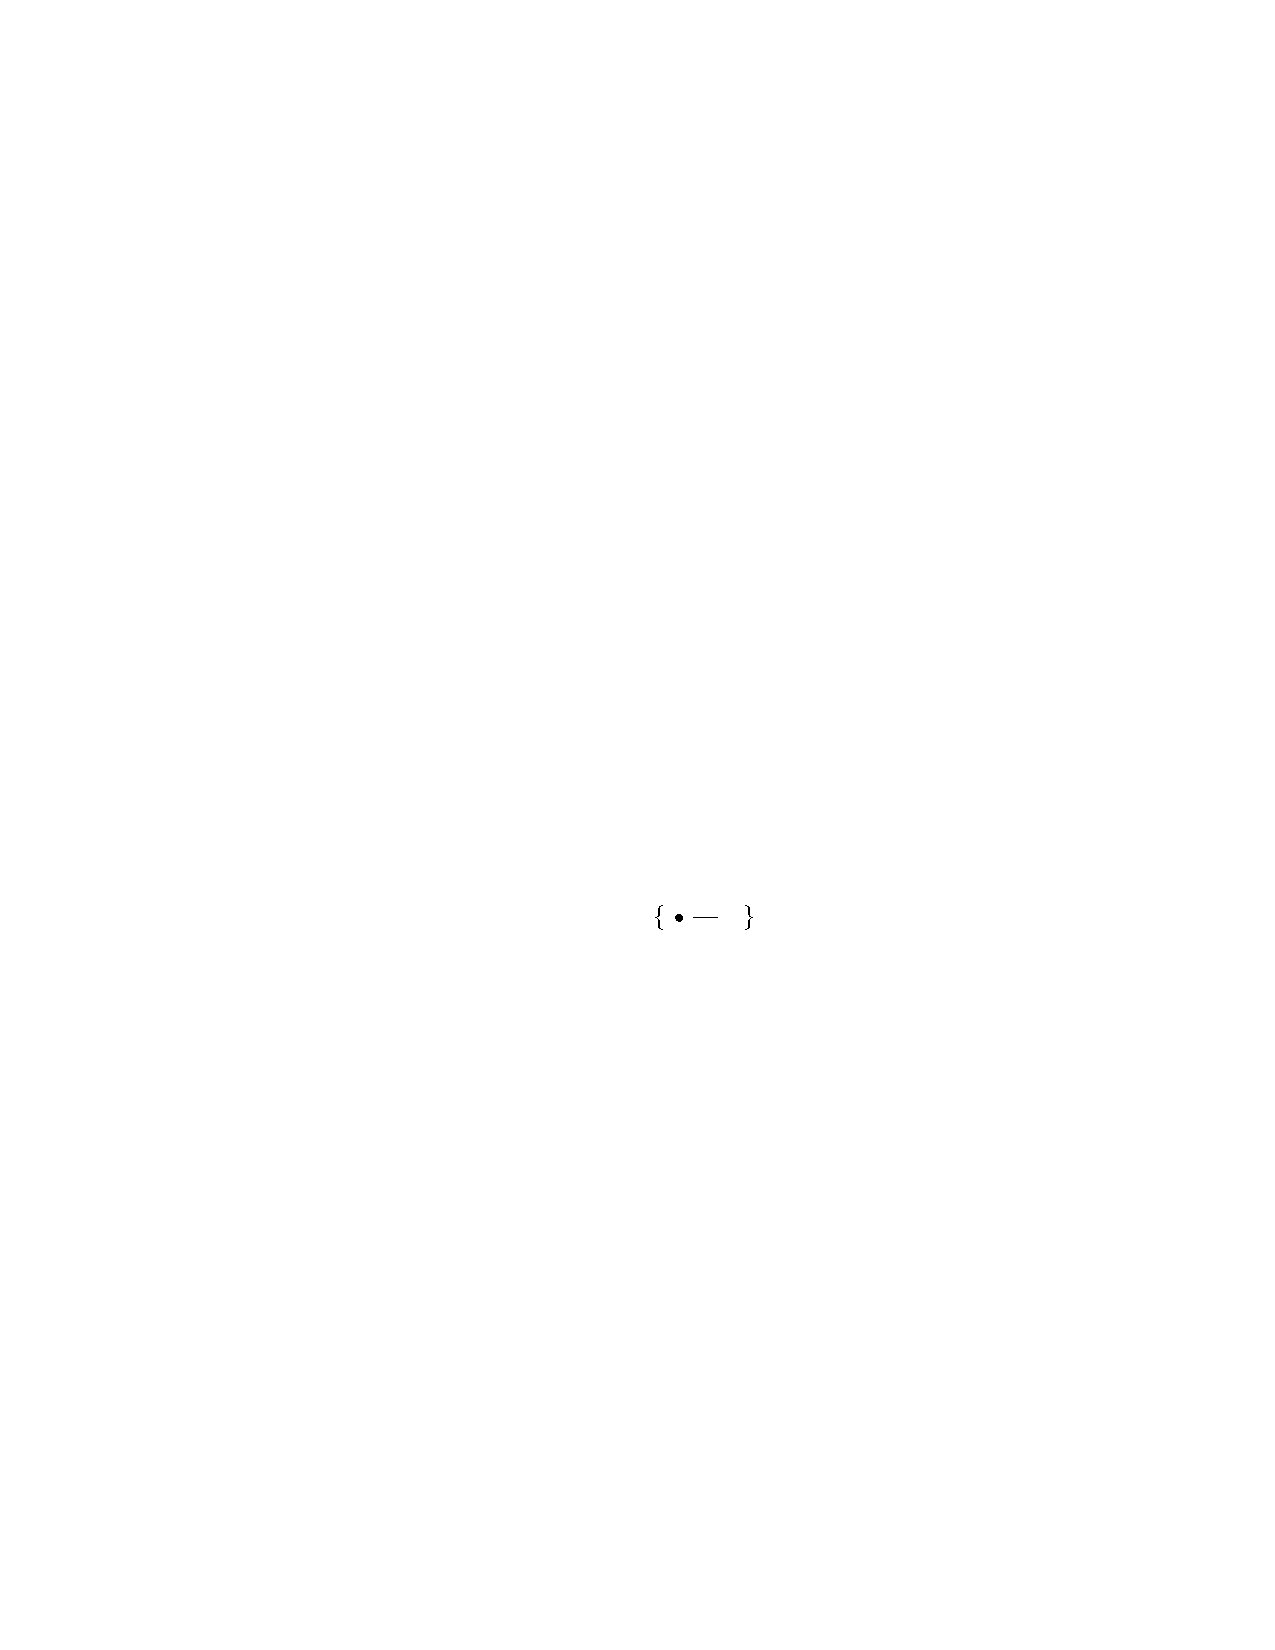
\includegraphics[width=0.1313\linewidth]{images/diagram-4-47a.pdf}}},\qquad\vcenter{\hbox{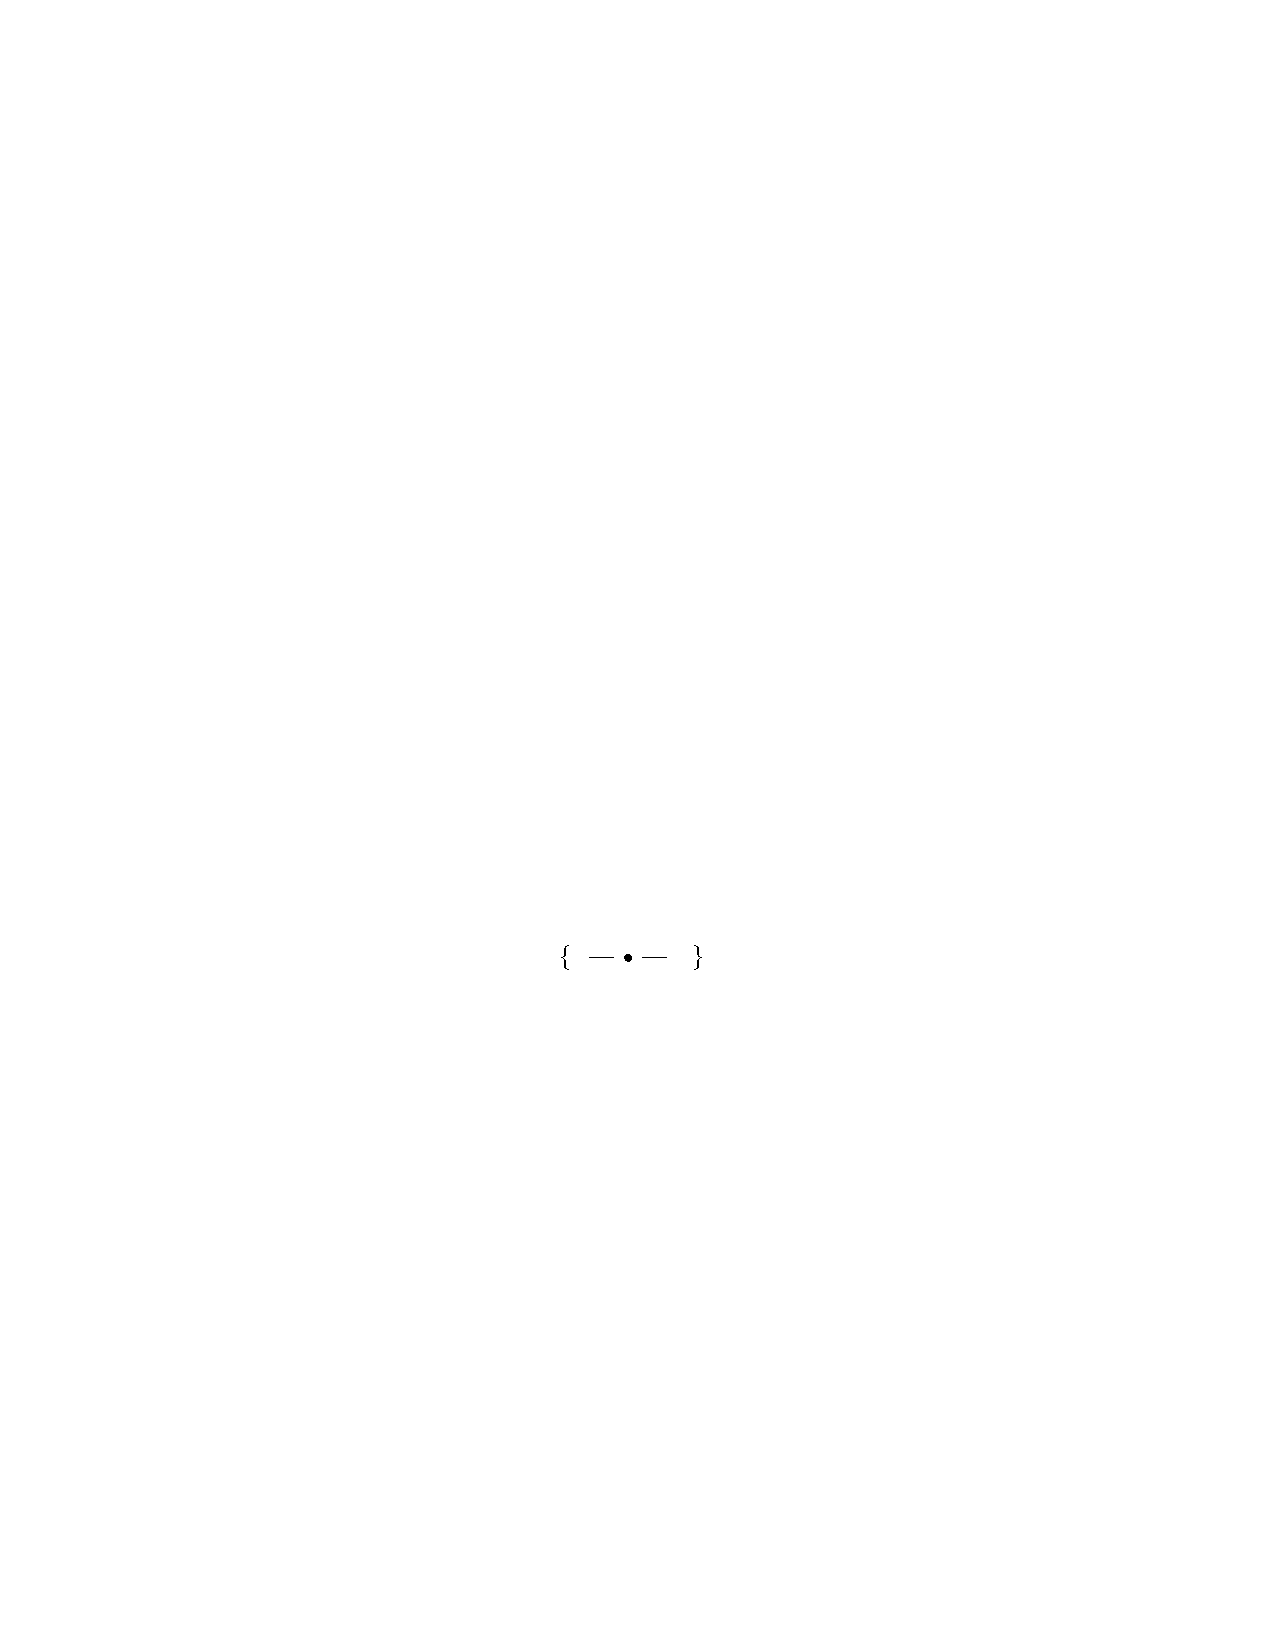
\includegraphics[width=0.1818\linewidth]{images/diagram-4-47b.pdf}}}.}
\end{example}
现在构造关联的概形。给定扇 $\Sigma$，对其中每个锥 $\sigma$，取仿射环面簇 $U_\sigma\supset\mathbb G_m^d$。对 $\sigma,\sigma'\in\Sigma$，不妨只考虑极大锥，其交是各自的面，所以有开嵌入
\Eq{4.48}{\begin{tikzcd}\&U_\sigma\\U_{\sigma\cap\sigma'}\arrow[ur,hook]\arrow[dr,hook]\&\\\&U_{\sigma'}.\end{tikzcd}}
于是
\Eq{4.49}{X(\Sigma)=\varinjlim_{\sigma\in\Sigma}U_\sigma}
是一个概形。我们将对 $\PP^2$ 显式检查这种相容性。
\section{例题：\texorpdfstring{$\PP^2$}{P²}}
设 $\Sigma$ 如例题~\ref{ex:4.10} 所示。对偶化得到图~\ref{fig:4.2} 中的锥。
\SourcePage{67}
\OriginalFigure{fig-4-2.pdf}{0.6498}{例题~\ref{ex:4.10} 中的扇所对应的对偶锥。}{fig:4.2}
这些锥给出如下开集：
\Eq{4.50}{U_{\sigma_0}=\Spec k[\underbrace{\chi^{(1,0)}}_{u_0},\underbrace{\chi^{(0,1)}}_{u_1}],}
\Eq{4.51}{U_{\sigma_1}=\Spec k[\underbrace{\chi^{(-1,1)}}_{v_0},\underbrace{\chi^{(-1,0)}}_{v_1}],}
\Eq{4.52}{U_{\sigma_2}=\Spec k[\underbrace{\chi^{(0,-1)}}_{w_0},\underbrace{\chi^{(1,-1)}}_{w_1}].}
现在把这些坐标图粘合起来。$\sigma_0\cap\sigma_1$ 是正 $y$ 轴，其对偶锥 $\sigma_0^\vee+\sigma_1^\vee$ 是上半平面，对应于
\Eq{4.53}{k[u_0,u_1]_{u_0}=k[v_0,v_1]_{v_1}.}
开嵌入 $U_{\sigma_0\cap\sigma_1}\hookrightarrow U_{\sigma_0}$ 对应于
\Eq{4.54}{k[u_0,u_1]\hookrightarrow k[u_0,u_1]_{u_0},}
而 $U_{\sigma_0\cap\sigma_1}\hookrightarrow U_{\sigma_1}$ 对应于
\Eq{4.55}{k[v_0,v_1]\hookrightarrow k[v_0,v_1]_{v_1}.}
二者确实一致。具体的坐标变换为
\Eq{4.56}{v_0=u_0^{-1}u_1,\qquad v_1=u_0^{-1}.}
因此得到
\Eq{4.57}{X(\Sigma)\simeq\PP^2=\operatorname{Proj}k[x_0,x_1,x_2],}
\SourcePage{68}
其中具体地，
\Eq{4.58}{u_0=x_1/x_0,\qquad u_1=x_2/x_0,}
\Eq{4.59}{v_0=u_0^{-1}u_1=(x_0/x_1)(x_2/x_0)=x_2/x_1,\qquad v_1=u_0^{-1}=x_0/x_1,}
\Eq{4.60}{w_0=u_1^{-1}=x_0/x_2,\qquad w_1=x_1/x_2.}
\section{作为环面簇的\texorpdfstring{$\PP_k^d$}{Pᵈ}}
对 $i\in\{1,\ldots,d\}$，记
\Eq{4.61}{v_i=e_i=(0,\ldots,0,1,0,\ldots,0)\in\RR^d,}
并令
\Eq{4.62}{v_0=-\sum_{i=1}^de_i=(-1,\ldots,-1).}
令 $\Sigma$ 为射线为 $\RR_{\ge0}v_i$ 的完备扇。
\Lecture{19}{2019年10月31日}
\section{环面分层}
设 $\Sigma$ 为扇，$\tau\in\Sigma$。它给出相应子环面的不动点闭子集。具体地，令 $N_\tau=N\cap\RR\tau$，$M_\tau=\Hom(N_\tau,\ZZ)$，$T_\tau=\Spec k[M_\tau]$。在 $\sigma\supseteq\tau$ 对应的坐标图内，取
\Eq{4.63}{\Spec(k[\sigma^\vee\cap M]^{T_\tau})=\Spec k[(\tau^\perp\cap\sigma^\vee)\cap M]\hookrightarrow\Spec k[\sigma^\vee\cap M],}
现在进行整体化。对 $N_{\RR}$ 中的扇 $\Sigma$ 和 $\tau\in\Sigma$，商空间 $N_{\RR}/\RR\tau$ 中有商扇
\Eq{4.64}{\Sigma_\tau=\{\sigma/\RR\tau:\sigma\in\Sigma,\ \sigma\supseteq\tau\}.}
它给出闭嵌入 $X(\Sigma_\tau)\subset X(\Sigma)$。若 $X(\Sigma)$ 的维数为 $d$，则 $X(\Sigma_\tau)$ 的维数为 $d-\dim\tau$。
\examnum{13}\begin{example}\label{ex:4.13}
取 $\PP^3$ 的扇，令 $\tau$ 为正 $z$ 轴所给出的射线，则其商扇给出 $\PP^2$。
\end{example}
射线与环面除子之间存在基本对应；这里环面除子指环面作用下不变的除子。其仿射坐标图由 $\sigma\supseteq\tau$ 给出，因为有
\Eq{4.65}{k[\sigma^\vee\cap M]\twoheadrightarrow k[\underbrace{\sigma^\vee\cap\tau^\perp}_{(\sigma/\RR\tau)^\vee}\cap M].}
\SourcePage{69}
\OriginalFigure{fig-4-3.pdf}{0.5101}{$N_{\RR}=\RR^2$ 中的一个无穷扇。}{fig:4.3}
\section{拟紧性}
\examnum{14}\begin{example}\label{ex:4.14}
考虑图~\ref{fig:4.3} 的扇。注意
\Eq{4.66}{|\Sigma|=(\RR\times\RR_{>0})\cup\{(0,0)\}\subset\RR^2}
不是闭集。它给出的环面簇为
\Eq{4.67}{X(\Sigma)=\bigcup_{\text{可数无穷}}\mathbb A^2,}
并不拟紧。通过无穷次吹起，可以得到：
\Eq{4.68}{X(\Sigma)\overset{\operatorname{Bl}_\infty}{\dashrightarrow}\mathbb A^1\times\mathbb G_m.}
记到 $\mathbb A^1$ 的投影为 $\pi$，则
\Eq{4.69}{\pi^{-1}(0)=\bigcup_{\text{可数无穷}}\PP^1,}
而对 $\mathbb A^1$ 的一般点 $\eta$，
\Eq{4.70}{\pi^{-1}(\eta)=\mathbb G_{m/k(t)}.}
\end{example}
于是得到：
\thmnum{proposition}{8}\begin{proposition}\label{prop:4.8}
$X(\Sigma)$ 拟紧当且仅当 $\Sigma$ 有限。
\end{proposition}
\begin{proof}
$\Leftarrow$ 显然。对 $\Rightarrow$，我们知道
\Eq{4.71}{\bigcup_{\tau\in\Sigma,\ \dim\tau=1}X(\Sigma_\tau)}
只有有限个不可约分支。因此一维锥 $\tau\in\Sigma$ 的数目有限，从而整个扇 $\Sigma$ 有限。
\end{proof}
\SourcePage{70}
\section{扇的态射}
\thmnum{definition}{8}\begin{definition}\label{def:4.8}
设 $\Sigma$、$\Sigma'$ 分别为格 $N$、$N'$ 中的扇。扇的态射 $\varphi:\Sigma\to\Sigma'$ 是线性映射 $\varphi:N_{\RR}\to N'_{\RR}$，满足 $\varphi(N)\subseteq N'$，且对每个 $\sigma\in\Sigma$，都存在 $\sigma'\in\Sigma'$ 使 $\varphi(\sigma)\subseteq\sigma'$。
\end{definition}
\begin{Note}{4.6}$\sigma'$ 不一定唯一，但其中存在唯一最小的一个。\end{Note}
\thmnum{definition}{9}\begin{definition}[环面态射的构造]\label{def:4.9}
扇态射 $\varphi:\Sigma\to\Sigma'$ 诱导 $\Phi:X(\Sigma)\to X(\Sigma')$，它相对于 $\mathbb G_m(N)\to\mathbb G_m(N')$ 的作用等变。其构造如下：局部取 $\sigma\in\Sigma$、$\sigma'\in\Sigma'$，满足 $\varphi(\sigma)\subseteq\sigma'$，再以环同态
\Eq{4.72}{\begin{aligned}\varphi^*:k[(\sigma')^\vee\cap M']&\longrightarrow k[\sigma^\vee\cap M],\\\chi^m&\longmapsto\chi^{\varphi^*(m)}\end{aligned}}
定义 $\Phi:U_\sigma\to U_{\sigma'}$。对偶配对给出相容关系
\Eq{4.73}{\begin{tikzcd}N_{\RR}\arrow[r,"{\varphi}"]\&N'_{\RR}\\\sigma\arrow[u,hook]\arrow[r,"{\varphi}"']\&\sigma'\arrow[u,hook]\arrow[r,"{m}"]\&\RR_{\ge0}.\end{tikzcd}}
\end{definition}
\begin{Note}{4.7}在仿射开集的层面上，$\Phi$ 非常简单；只需选取一组基写出它即可。\end{Note}
\begin{Note}{4.8}映射 $\mathbb G_m(N)\to\mathbb G_m(N')$ 把单位元 $e=Z(\chi^m-1)_{m\in M}$ 映到单位元 $e'=Z(\chi^{m'}-1)_{m'\in M'}$。\end{Note}
\section{例题}
\examnum{15}\begin{example}\label{ex:4.15}
取 $N_{\RR}=\RR$、$N'_{\RR}=\RR^2$，用 $\lambda\mapsto(p\lambda,q\lambda)$ 定义映射，其中 $p,q$ 为正整数。对偶格映射 $M'=\ZZ^2\to M=\ZZ$ 把 $(m_1,m_2)$ 映为 $pm_1+qm_2$。在相应坐标环上，
\Eq{4.74}{\begin{aligned}k[x,y]&\longrightarrow k[u],\\x&\longmapsto u^p,\qquad y\longmapsto u^q.\end{aligned}}
若 $\gcd(p,q)=1$，则此环同态的核为 $(x^q-y^p)$。$T_N$ 在 $T_{N'}=\mathbb G_m^2$ 中的像，在 $\mathbb A^2$ 中的闭包就是 $Z(x^q-y^p)$。
\end{example}
\examnum{16}\begin{example}\label{ex:4.16}
取 $\RR^2$ 中由 $(1,0),(1,1)$ 生成的锥 $\sigma$，并取
\Eq{4.75}{N_{\RR}=\RR^2\xrightarrow{\varphi=\id}N'_{\RR}=\RR^2,}
\SourcePage{71}
靶锥则为 $\sigma'=\RR_{\ge0}^2$。$\sigma^\vee$ 由 $(1,-1),(0,1)$ 张成，而 $(\sigma')^\vee=\RR_{\ge0}^2$。从 $(\sigma')^\vee$ 到 $\sigma^\vee$ 的映射，在幺半群环上为
\Eq{4.76}{x=\chi^{(1,0)}\longmapsto uv,\qquad y=\chi^{(0,1)}\longmapsto v,}
这是原点吹起 $\operatorname{Bl}_0\mathbb A^2\to\mathbb A^2$ 的一个仿射坐标图：
\Eq{4.77}{\operatorname{Bl}_{(x,y)}\mathbb A^2=\operatorname{Proj}\frac{\underbrace{k[x,y]}_{\deg=0}[\underbrace{U,V}_{\deg=1}]}{(xV-yU)}.}
现在作去齐次化，即考虑 $U\ne0$ 与 $V\ne0$ 两个坐标图。为消去 $y$，令 $U=1$、$v=V/U$，得到
\Eq{4.78}{k[x,y]\longrightarrow k[x,v],\qquad x\longmapsto x,\quad y\longmapsto xv.}
类似地，在 $V\ne0$ 的坐标图上，令 $V=1$、$u=U/V$，为消去 $x$，得到
\Eq{4.79}{k[x,y]\longrightarrow k[y,u],\qquad x\longmapsto yu,\quad y\longmapsto y.}
\end{example}
\thmnum{definition}{10}\begin{definition}\label{def:4.10}
扇的细分是一个扇态射 $\widetilde\Sigma\to\Sigma$，其格映射为恒等映射 $N\xrightarrow{\id}N=N'$，并且对靶扇中的每个 $\sigma'$，都有
\Eq{4.80}{\sigma'=\bigcup_{\sigma\subseteq\varphi^{-1}(\sigma')}\varphi(\sigma).}
\end{definition}
因此，有限扇的细分对应于一个修正，即双有理固有态射 $X(\widetilde\Sigma)\to X(\Sigma)$。
\examnum{17}\begin{example}\label{ex:4.17}
考虑 $N_{\RR}=\RR^2$ 中由 $(0,1),(k,1)$ 张成的锥 $\sigma$，其中 $k\ge1$。到 $y$ 轴的投影取值于 $N'_{\RR}=\RR$，把它映到由 $1$ 生成的锥 $\sigma'$。$\sigma^\vee$ 由 $(-1,k),(1,0)$ 生成，而 $(\sigma')^\vee$ 仍由 $1$ 生成。对偶映射把 $1$ 映为 $(0,1)$，故有
\Eq{4.81}{k[t]\longrightarrow k[x,y,t]/(xy-t^k),\qquad t=\chi^1\longmapsto\chi^{(0,1)}=t,}
\SourcePage{72}
其中 $x=\chi^{(1,0)}$、$y=\chi^{(-1,k)}$、$t=\chi^{(0,1)}$。这就是所谓的 $A_{k-1}$ 曲面奇点。它由一族曲线 $\{C_t\}$ 纤维化：$t\ne0$ 时 $C_t\simeq\mathbb G_m$ 光滑，而 $C_0=\mathbb A^1\cup\mathbb A^1$ 是结点曲线。
\end{example}
\examnum{18}\begin{example}[格的改变]\label{ex:4.18}
考虑 $N_{\RR}=\RR^2\to N'_{\RR}=\RR^2$，其矩阵为
\Eq{4.82}{\begin{pmatrix}a&0\\0&b\end{pmatrix}.}
对正整数 $a,b$，它对应于环同态
\Eq{4.83}{k[x,y]\longrightarrow k[x,y],\qquad x\longmapsto x^a,\quad y\longmapsto y^b.}
在特征零时，这是沿 $x$ 轴分歧指数为 $b$、沿 $y$ 轴分歧指数为 $a$ 的覆盖。
一般地，有限指数的格改变给出 $X(\Sigma')$ 的有限覆盖，分歧发生在环面分层上；分歧指数可从格映射 $N\to N'$ 的余核读出。
\end{example}
\examnum{19}\begin{example}\label{ex:4.19}
令 $\tau\in\Sigma$，并取 $N_\tau=N\cap\RR\tau$。考虑由 $\tau$ 及其所有面组成的扇
\Eq{4.84}{\Sigma(\tau)=\{\text{$\tau$ 的各个面，位于 }(N_\tau)_{\RR}=\RR\tau\text{ 中}\}.}
有自然映射
\Eq{4.85}{\begin{tikzcd}\Sigma(\tau)\arrow[r]\&\Sigma\\N_\tau\arrow[r,hook]\arrow[u]\&N\arrow[u].\end{tikzcd}}
它给出一个仿射环面子簇。具体地，
\Eq{4.86}{X(\Sigma(\tau))=\Spec k[(\tau\subset(N_\tau)_{\RR})^\vee\cap M_\tau]\longrightarrow X(\Sigma).}
\end{example}
\examnum{20}\begin{example}\label{ex:4.20}
作为上述例子的一个特例，取 $\PP^2$，令 $\tau$ 为一条射线。则
\Eq{4.87}{T_{N_\tau}=\{g\in T_N:\text{对所有 }p\in X(\Sigma_\tau),\ g\cdot p=p\}}
是逐点固定相应分层的子环面。现在考虑此子环面作用下，稠密环面中单位点的轨道在 $U_\tau$ 内的闭包。此闭包是仿射的，包含 $[1,0,1]$ 与 $[1,1,1]$，却不包含 $[0,1,0]$。
选取格的一个分解后，横向仿射环面簇与补环面的乘积给出
\Eq{4.88}{X(\Sigma(\tau))\times T_{N/N_\tau}\simeq U_\tau\subset X(\Sigma).}
因此，局部结构是一个环面与这个仿射簇的乘积。
\end{example}
\Lecture{20}{2019年11月5日}
\SourcePage{73}
\section{环面态射的性质}
采用记号 $X(\Sigma)=\mathrm{TV}(\Sigma,N)$。对 $\varphi:\Sigma\to\Sigma'$，记诱导态射为 $\Phi:X(\Sigma)\to X(\Sigma')$。
\thmnum{proposition}{9}\begin{proposition}\label{prop:4.9}
\begin{enumerate}[label=(\alph*)]
\item $\Phi$ 为闭嵌入，当且仅当
\Eq{4.89}{\Sigma=\{\varphi^{-1}(\sigma'):\sigma'\in\Sigma'\},}
这特别要求 $\varphi:N_{\RR}\to N'_{\RR}$ 单射，并且对每个 $\sigma'\in\Sigma'$、$\sigma=\varphi^{-1}(\sigma')$，半群映射
\Eq{4.90}{(\sigma')^\vee\cap M'\twoheadrightarrow\sigma^\vee\cap M}
为满射。
\item $\Phi$ 占优\footnote{回忆，这意味着它的像稠密。}当且仅当 $N'/\varphi(N)$ 为挠群；等价地，$[N':\varphi(N)]<\infty$。
\item $\Phi$ 总是分离的。
\item 在有限扇的情形，$\Phi$ 固有当且仅当 $\varphi^{-1}(|\Sigma'|)=|\Sigma|$。
\end{enumerate}
\end{proposition}
注意，删去极大锥通常就不会得到固有态射。前两个结论很容易，后两个则由赋值判别准则得到。
\section{环面簇的范畴}
目前，我们把环面簇定义为由上述扇构造产生的簇，把其态射定义为由扇态射诱导的态射。这是一种省事的定义。现在给出更内蕴的定义。
\thmnum{definition}{11}\begin{definition}\label{def:4.11}
基域 $k$ 上的环面簇是一个分离的有限型 $k$ 概形，它连通且正规，因而约化且不可约；同时带有代数环面 $T_N=\Spec k[N^*]$ 的作用，以及一个 $T_N$ 等变开嵌入 $T_N\hookrightarrow X$。
\end{definition}
设 $T_N\curvearrowright X$、$T_{N'}\curvearrowright X'$ 为环面簇。环面簇的态射由下列等变图给出：
\Eq{4.91}{\begin{tikzcd}T_N\arrow[r]\arrow[d,hook]\&T_{N'}\arrow[d,hook]\\X\arrow[r]\&X'.\end{tikzcd}}
注意，上方的环面群同态等价于格同态 $N\to N'$。
\thmnum{theorem}{10}\begin{theorem}\label{thm:4.10}
环面簇的范畴与有限扇的范畴等价。
\end{theorem}
\section{多胞体与多面体}
\thmnum{definition}{12}\begin{definition}\label{def:4.12}
向量空间 $V$ 中的凸\Term{duomianti}{多面体} $\Xi\subseteq V$ 是有限个闭半空间的交。
\end{definition}
\thmnum{definition}{13}\begin{definition}\label{def:4.13}
\Term{duobaoti}{多胞体}是有限个点的凸包。
\end{definition}
注意，这意味着多胞体有界。取 $V=M_{\RR}$、$M=\ZZ^n$。若多胞体由 $v_i\in M_{\QQ}$ 的凸包给出，则称它有理；若各 $v_i\in M$，则称它整。多面体称为有理，是指它可由有限个 $\langle u,x\rangle\ge a$ 的半空间定义，其中 $u\in M^*\otimes_{\ZZ}\QQ=N_{\QQ}$、$a\in\QQ$。
\thmnum{theorem}{11}\begin{theorem}\label{thm:4.11}
多胞体恰好就是有界多面体。
\end{theorem}
\SourcePage{74}
\OriginalFigure{fig-4-4.pdf}{0.5126}{例题~\ref{ex:4.21} 中的多面体 $\Xi$。}{fig:4.4}
多面体和多胞体也有如前所述的面；余维一面称为侧面。它们还有顶点，但无界多面体可能没有顶点。
设 $\Xi\subset M_{\RR}$ 为多面体，可以构造其上方的锥
\Eq{4.92}{C(\Xi)=\overline{\{(m,h)\in M_{\RR}\times\RR:h>0,\ m\in h\Xi\}}.}
若不取闭包，则无界多面体上方的锥未必是闭的。$\Xi$ 的\Term{huishouzhui}{回收锥}，也称渐近锥，就是 $C(\Xi)\cap(M_{\RR}\times\{0\})$，并把它看作 $M_{\RR}$ 的子集。
\examnum{21}\begin{example}\label{ex:4.21}
取 $M_{\RR}=\RR^2$，$\Xi$ 如图~\ref{fig:4.4}。现在构造其上方的锥；高度零处的截面就是一个象限。
\end{example}
\thmnum{definition}{14}\begin{definition}[对偶多胞体与多面体]\label{def:4.14}
设 $\Xi\subset M_{\RR}$，且 $0$ 在 $\Xi$ 的内部。其对偶（极）多面体定义为
\Eq{4.93}{\Xi^\circ=\{v\in N_{\RR}:\text{对所有 }u\in\Xi,\ \langle u,v\rangle\le1\}.}
\end{definition}
\begin{Note}{4.9}稍后将由这些对象构造 Calabi–Yau 簇，而这一对偶操作就是镜像对称。\end{Note}
\begin{Note}{4.10}我们希望有 $C(\Xi)^\vee=C(-\Xi^\circ)$。\end{Note}
\begin{Note}{4.11}这里有约定的选择：也可以改用 $\langle u,v\rangle\ge-1$，得到的多面体就是当前对偶多面体的负。\end{Note}
注意，不包含在 $M_{\RR}\times\{0\}$ 内的真面 $\tau\subset C(\Xi)$，与 $\Xi$ 的真面一一对应。
\examnum{22}\begin{example}\label{ex:4.22}
考虑图~\ref{fig:4.5} 中的多胞体，图中也画出了它的对偶多胞体。
\end{example}
\examnum{23}\begin{example}\label{ex:4.23}
考虑立方体
\Eq{4.94}{\Xi=\conv\{(\pm1,\pm1,\pm1)\}.}
\SourcePage{75}
\OriginalFigure{fig-4-5.pdf}{0.5909}{$\RR^2$ 中的多胞体及其对偶多胞体。}{fig:4.5}
其对偶为
\Eq{4.95}{\Xi^\circ=\conv\{\pm e_1,\pm e_2,\pm e_3\},}
即一个八面体。
\end{example}
\section{由多面体构造环面簇}
考虑满维凸有理多面体 $\Xi\subset M_{\RR}$。对其面 $\Xi'\subseteq\Xi$，令
\Eq{4.96}{\sigma_{\Xi'}=\{v\in N_{\RR}:\langle u-u',v\rangle\ge0\text{ 对所有 }u\in\Xi,\ u'\in\Xi'\},}
\Eq{4.97}{\sigma_{\Xi'}=\left(\overline{\RR_{\ge0}\{u-u':u\in\Xi,\ u'\in\Xi'\}}\right)^\vee.}
\thmnum{proposition}{12}\begin{proposition}\label{prop:4.12}
\begin{enumerate}[label=(\alph*)]
\item
\Eq{4.98}{\Sigma_\Xi=\{-\sigma_{\Xi'}:\Xi'\subseteq\Xi\text{ 为面}\}}
\SourcePage{76}
是 $N_{\RR}=M_{\RR}^*$ 中的扇，称为 $\Xi$ 的\Term{fashan}{法扇}。$\Sigma_\Xi$ 完备当且仅当 $\Xi$ 有界。
\item 若 $0$ 在 $\Xi$ 的内部，则
\Eq{4.99}{\Sigma_\Xi=\{\{0\}\}\cup\{\RR_{\ge0}F:F\subsetneq\Xi^\circ\text{ 为面}\}.}
\end{enumerate}
\end{proposition}
\OriginalFigure{fig-4-6.pdf}{0.5067}{例题~\ref{ex:4.24} 中的法扇 $\Sigma_\Xi$。}{fig:4.6}
\examnum{24}\begin{example}\label{ex:4.24}
考虑下列多胞体：
\Eq{4.100}{\vcenter{\hbox{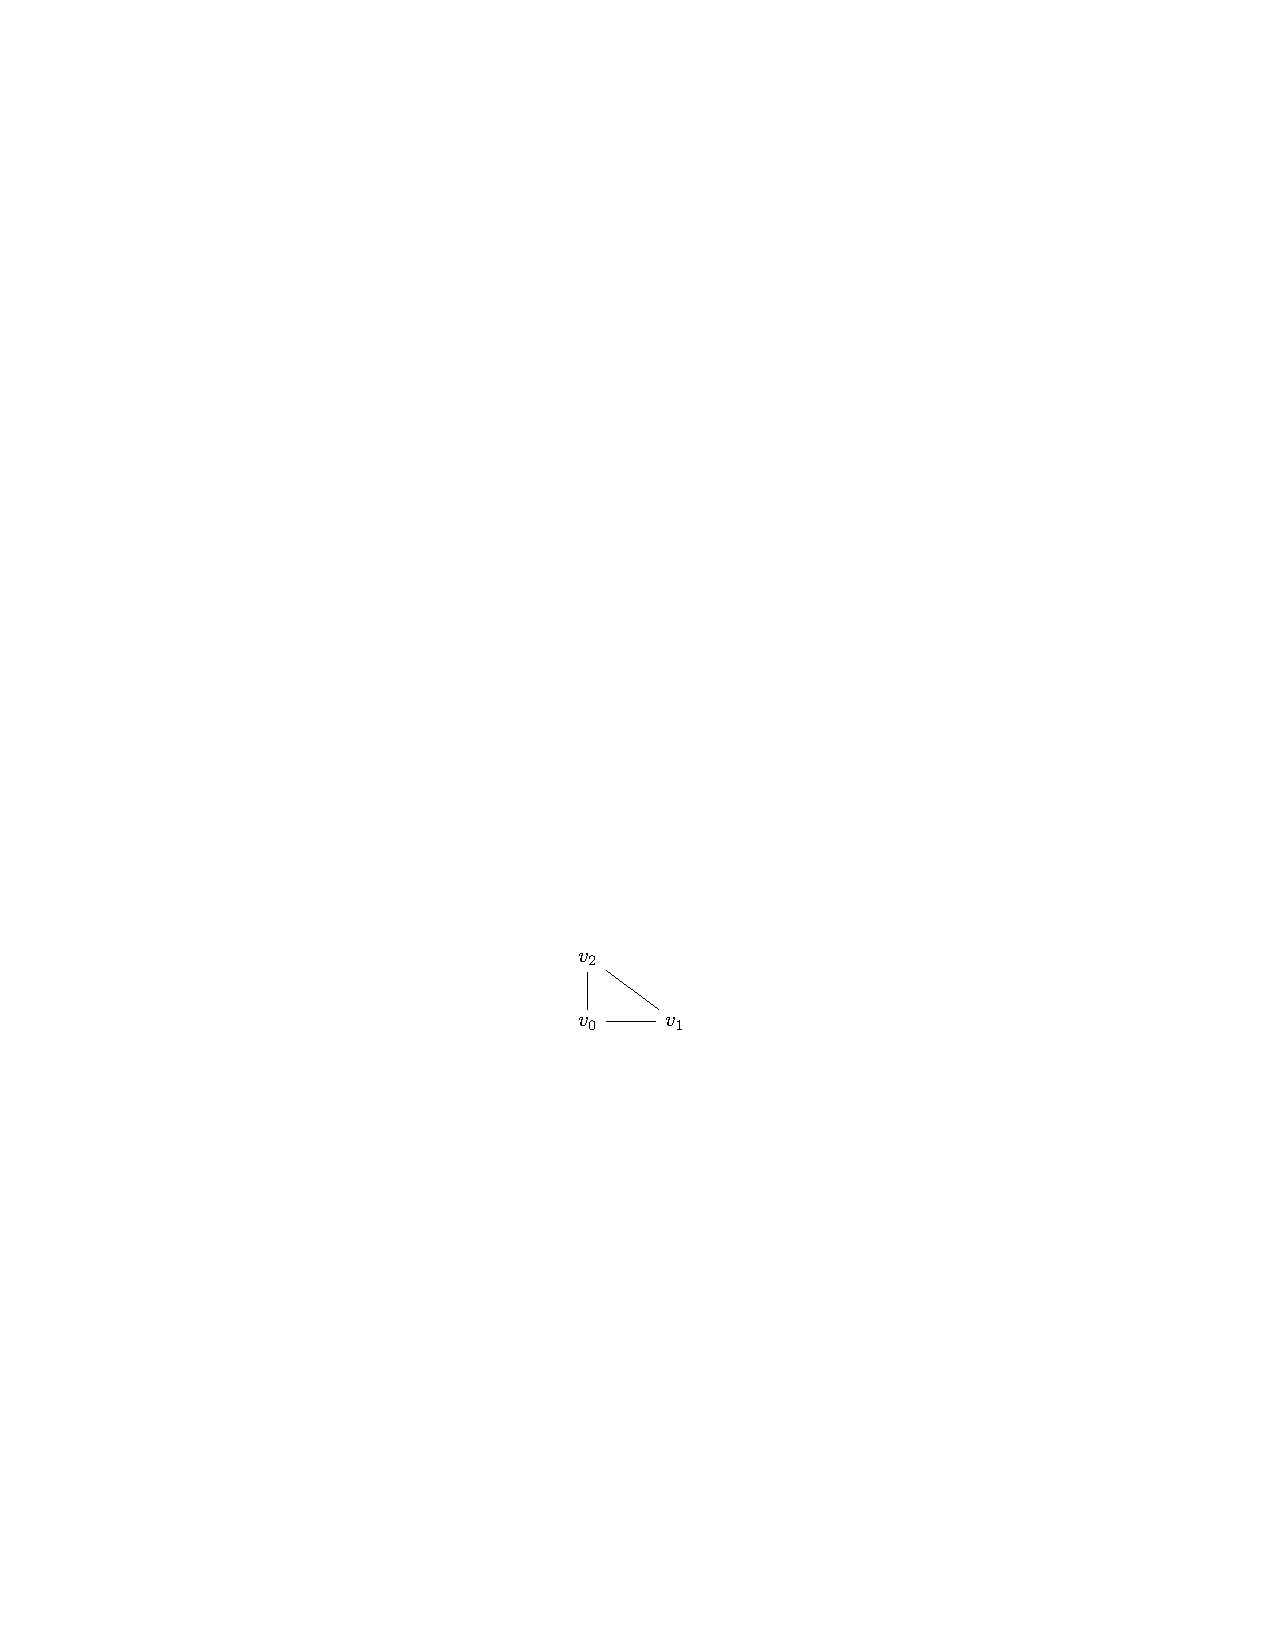
\includegraphics[width=0.1364\linewidth]{images/diagram-4-100.pdf}}}.}
每个顶点 $v_i$ 对应一个锥 $\tau_i$。它们正好是图~\ref{fig:4.1} 中的三个锥，因此 $\Sigma_\Xi$ 如图~\ref{fig:4.6} 所示。
\end{example}
\begin{Note}{4.12}把 $\Xi$ 按正比例缩放，或对它的各个面作保持组合类型的小幅平行移动，均不改变法扇。\end{Note}
\thmnum{definition}{15}\begin{definition}\label{def:4.15}
与 $\Xi$ 关联的环面簇定义为 $X(\Sigma_\Xi)$。
\end{definition}
\examnum{25}\begin{example}\label{ex:4.25}
若
\Eq{4.101}{\Xi=\conv\{0,e_1,\ldots,e_d\},}
则 $X(\Sigma_\Xi)\simeq\PP^d$。当 $d=2$ 时，除去缩放与平移，这就是例题~\ref{ex:4.24}：取 $(0,0),(0,1),(1,0)$ 的凸包，可得到例题~\ref{ex:4.10} 中的 $\PP^2$。当 $d=3$ 时，相应多胞体是四面体。
\end{example}
\SourcePage{77}
\OriginalFigure{fig-4-7.pdf}{0.5202}{在此图上方取锥得到一个扇，它有7个极大锥。}{fig:4.7}
\examnum{26}\begin{example}\label{ex:4.26}
回忆 Hirzebruch 曲面 $X=\PP(\OO_{\PP^1}\oplus\OO_{\PP^1}(a))$，其中 $a\ge0$。它由 $X(\Sigma_\Xi)$ 给出，$\Xi$ 为如下梯形：
\Eq{4.102}{\vcenter{\hbox{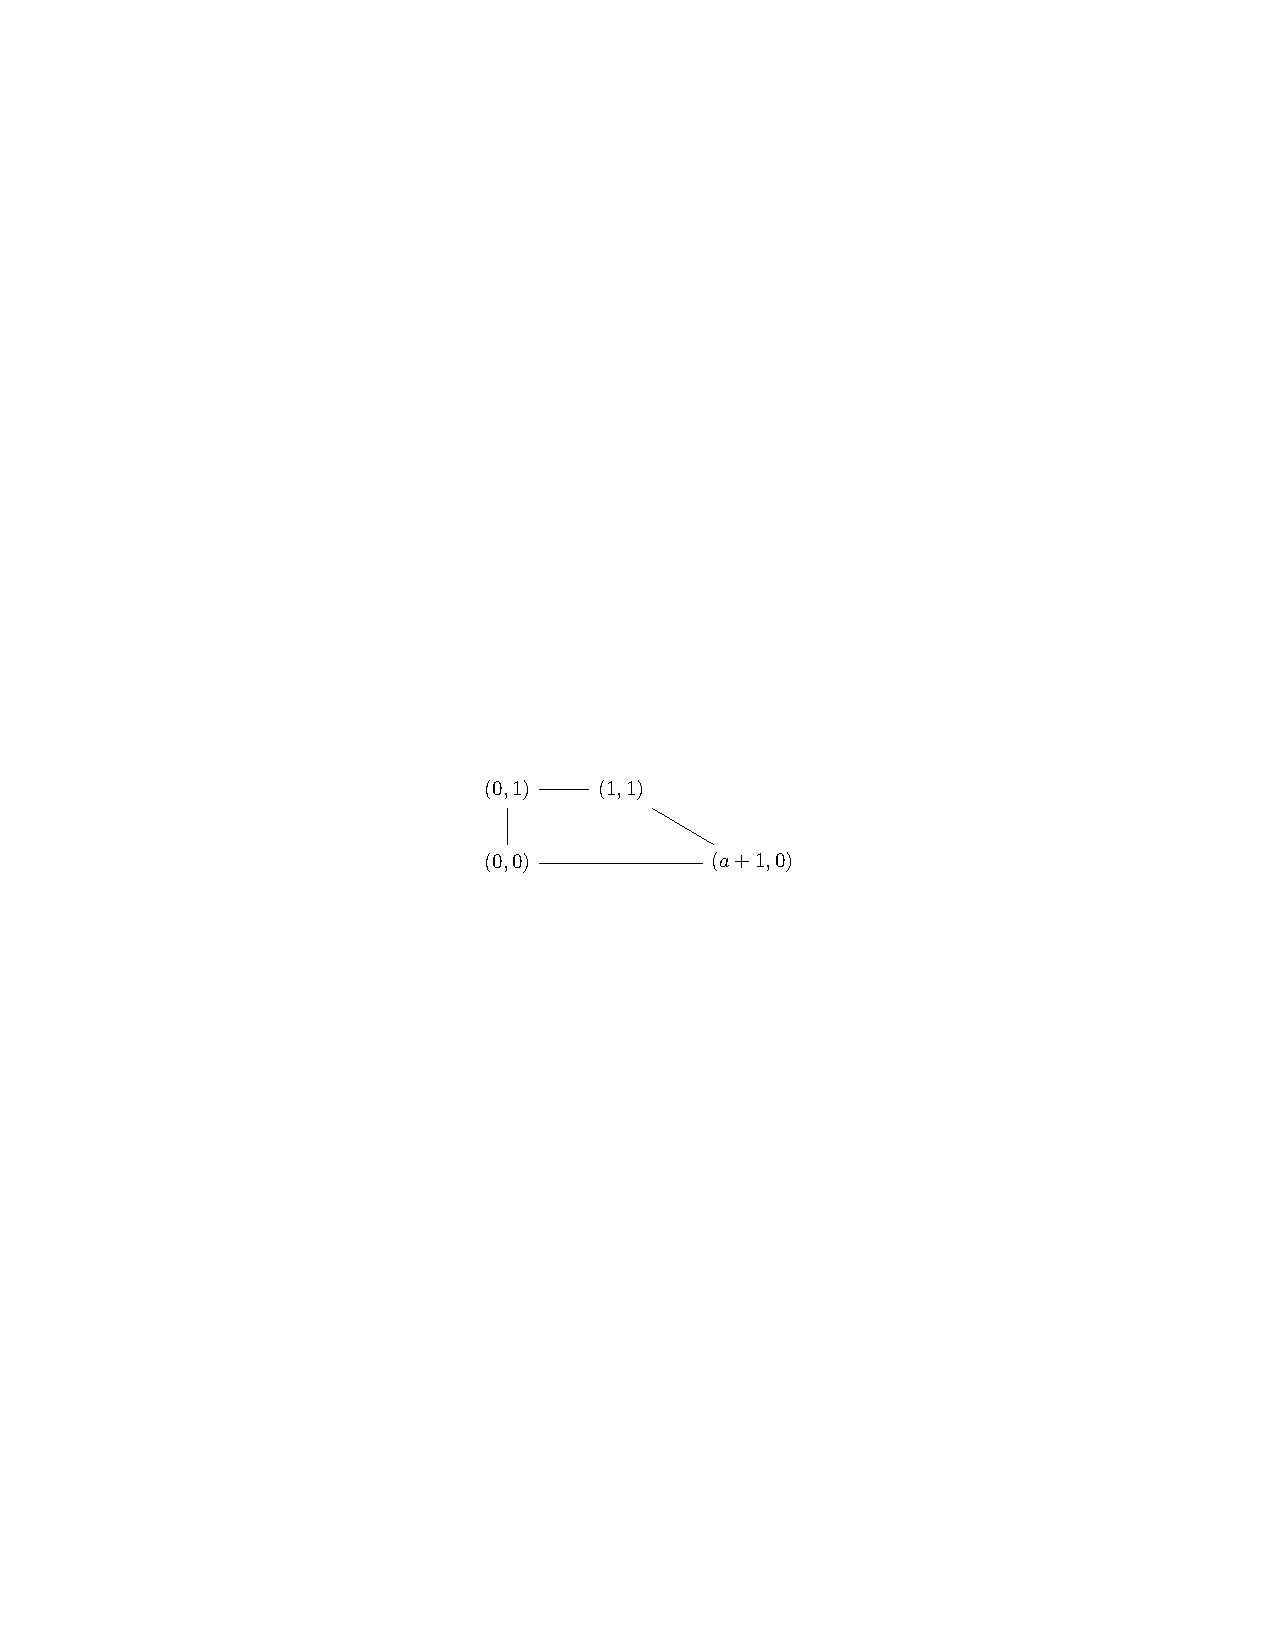
\includegraphics[width=0.3847\linewidth]{images/diagram-4-102.pdf}}}.}
\end{example}
\Lecture{21}{2019年11月7日}
\thmnum{proposition}{13}\begin{proposition}\label{prop:4.13}
$\operatorname{Proj}k[C(\Xi)\cap(M\oplus\ZZ)]\simeq X(\Sigma_\Xi)$。
\end{proposition}
\begin{proof}
一旦理解这个 $\operatorname{Proj}$ 的构造，结论便是同义反复。具体地，在单项式 $\chi^{(v,1)}$ 处作去齐次化，会得到形如 $\Spec k[\sigma^\vee\cap M]$ 的开集，于是结论成立。
\end{proof}
\begin{Note}{4.13}有如下典范双射：
\Eq{4.103}{\left\{\text{满维有理多面体 }\Xi\subset M_{\RR}\right\}\simeq\left\{(\Sigma,\varphi):\begin{array}{l}\Sigma\text{ 是 }N_{\RR}\text{ 中支撑凸的扇},\\\varphi:|\Sigma|\to\RR\text{ 是有理、严格凸的分段线性函数}\end{array}\right\}.}
特别地，左侧的顶点 $v_i$ 对应右侧的极大锥 $\sigma$，且 $\varphi|_\sigma=v_i:N_{\RR}\to\RR$。反向映射把 $\varphi$ 送到 $(\Sigma,\varphi)$ 的 Newton 多面体，记为 $\Xi(\Sigma,\varphi)$。$\Xi\mapsto\Xi+m$ 对应于 $(\Sigma,\varphi)\mapsto(\Sigma,\varphi+m)$。
\end{Note}
\begin{Note}{4.14}并非每个扇都能这样得到。二维时每个有限扇都可以支持相应的严格凸分段线性函数；三维及更高维则不然。\end{Note}
\begin{Counterexample}{2}\label{counterex:2}
在图~\ref{fig:4.7} 上方取锥。所得扇不能支持严格凸的分段线性函数；等价地，该三角剖分不是“正则”的。
\end{Counterexample}
\examnum{27}\begin{example}\label{ex:4.27}
回忆例题~\ref{ex:4.21}，其上方的锥为
\Eq{4.104}{C(\Xi)=\langle(1,0,0),(0,1,0),(1,0,1),(0,1,1)\rangle.}
\SourcePage{78}
于是
\Eq{4.105}{k[C(\Xi)\cap(M\oplus\ZZ)]\simeq k[x,y][U,V]/(xV-yU).}
取 $\operatorname{Proj}$，得到吹起
\Eq{4.106}{\operatorname{Proj}k[C(\Xi)\cap(M\oplus\ZZ)]\simeq\operatorname{Bl}_0\mathbb A^2.}
从扇的角度看，先取给出 $\mathbb A^2$ 的右上象限，再把它细分为由 $(1,0),(1,1)$ 生成的锥，以及由 $(1,1),(0,1)$ 生成的锥。关键在于，截去多面体的角对应于其法扇 $\Sigma_\Xi$ 的射影细分。\footnote{即细分支持一个严格凸的分段线性函数。}
\end{example}
\section{环面簇上的 Weil 除子}
设 $X$ 为 $d$ 维环面簇，扇为 $\Sigma$，射线为 $\RR_{\ge0}v_1,\ldots,\RR_{\ge0}v_r$，各 $v_i$ 均为本原向量。每个 $v_i$ 给出一个 $d-1$ 维环面分层，即 Weil 除子 $D_i$，称为环面素除子。记
\Eq{4.107}{\operatorname{Div}^T X\subset\operatorname{Div}X}
为 $T$ 不变 Weil 除子的子群。注意，
\Eq{4.108}{\operatorname{Div}^T X=\bigoplus_{i=1}^r\ZZ[D_i].}
\Term{chuzileiqun}{除子类群}为
\Eq{4.109}{\operatorname{Cl}X=A_{d-1}(X)=\operatorname{Div}X/{\sim_{\text{有理等价}}}.}
\thmnum{proposition}{14}\begin{proposition}\label{prop:4.14}
以下序列正合：
\Eq{4.110}{0\longrightarrow M/(M\cap|\Sigma|^\perp)\xrightarrow{m\mapsto\operatorname{div}(\chi^m)}\operatorname{Div}^T X\longrightarrow\operatorname{Cl}X\longrightarrow0,}
其中
\Eq{4.111}{\operatorname{div}(\chi^m)=\sum_{i=1}^r\operatorname{ord}_{D_i}(\chi^m)D_i.}
\end{proposition}
\begin{proof}
$k[M]$ 是唯一分解整环，因而
\Eq{4.112}{0=\operatorname{Cl}\Spec k[M]=\operatorname{Cl}T=\operatorname{Cl}(X\setminus D).}
由此 $A_{d-1}(D)=\operatorname{Div}^T(X)\twoheadrightarrow\operatorname{Cl}X$。
若 $\sum n_iD_i$ 在此映射的核中，则存在 $f\in k(X)^\times$，使 $\operatorname{div}(f)=\sum n_iD_i$。这意味着
\Eq{4.113}{f|_{X\setminus D}\in k[M]^\times=k^\times\times M,}
即 $f=\lambda\chi^m$，其中 $\lambda\in k^\times$、$m\in M$。不妨令 $\lambda=1$。
\end{proof}
\SourcePage{79}
注意 $\operatorname{ord}_{D_i}\chi^m=\langle v_i,m\rangle$。为说明这一点，选取 $N$ 的格基，令第一个基向量为 $e_1=v_i$，其余基向量任意补齐。记对偶基为 $e_j^*$，则 $D_i$ 中的稠密环面为
\Eq{4.114}{T_{D_i}=\Spec k[\chi^{\pm e_2^*},\ldots,\chi^{\pm e_d^*}],}
它位于开集
\Eq{4.115}{X\supset U_i=\Spec k[\chi^{e_1^*},\chi^{\pm e_2^*},\ldots,\chi^{\pm e_d^*}].}
写 $m=\sum_jm_je_j^*$，则 $\chi^m=\prod_j(\chi^{e_j^*})^{m_j}$，因此
\Eq{4.116}{\operatorname{ord}_{D_i}\chi^m=m_1=\langle m,v_i\rangle.}
\section{\texorpdfstring{$\operatorname{Cl}(\PP^n)$}{Cl(Pⁿ)}}
\thmnum{corollary}{15}\begin{corollary}\label{cor:4.15}
$\operatorname{Cl}(\PP^n)=A_{n-1}(\PP^n)=\ZZ H$，其中 $H$ 是一个超平面。次数映射 $\operatorname{Cl}(\PP^n)\to\ZZ$ 由与直线相交给出。
\end{corollary}
\begin{proof}
有短正合序列
\Eq{4.117}{0\longrightarrow\ZZ^n\xrightarrow{m\mapsto(\langle v_i,m\rangle)_i}\ZZ^{n+1}\xrightarrow{(a_i)\mapsto\sum_i a_i}\ZZ\longrightarrow0,}
而相应射线为
\Eq{4.118}{\Sigma_{\PP^n}[1]=\{\RR_{\ge0}e_1,\ldots,\RR_{\ge0}e_n,\RR_{\ge0}(-e_1-\cdots-e_n)\}.}
\end{proof}
\section{环面簇上的 Cartier 除子}
回忆，Cartier 除子群为
\Eq{4.119}{\operatorname{CaDiv}X=\Gamma(X,\mathcal K^\times/\OO_X^\times),}
其中 $\mathcal K$ 为全商环层。若 $X$ 整，则 $\mathcal K$ 是茎为函数域 $K(X)$ 的常值层。于是 Cartier 除子可由数据
\Eq{4.120}{\{(U_i,f_i):f_i\in K(X)^\times,\ f_i/f_j\in\OO_X^\times(U_i\cap U_j)\text{ 对所有 }i,j\}}
表示，并有 $\operatorname{CaDiv}X\hookrightarrow\operatorname{Div}X$。
\thmnum{lemma}{16}\begin{lemma}\label{lem:4.16}
设 $X=\Spec k[\sigma^\vee\cap M]$ 为仿射环面簇。$T$ 不变 Weil 除子 $D$ 是 Cartier 除子，当且仅当存在 $m\in M$ 使 $D=\operatorname{div}(\chi^m)$。
\end{lemma}
\thmnum{proposition}{17}\begin{proposition}\label{prop:4.17}
设 $\Sigma$ 为 $N_{\RR}$ 中的扇，相应环面簇为 $X_\Sigma$。则
\Eq{4.121}{\operatorname{CaDiv}^T(X_\Sigma)\simeq\mathrm{PL}(\Sigma)=\{\varphi:|\Sigma|\to\RR:\varphi\text{ 在每个锥上由 }M\text{ 中的线性函数给出}\}.}
此对应把 $\varphi$ 映为 $\sum_i\varphi(v_i)D_i$，其中 $v_i$ 为射线的本原生成向量，射线写成 $\RR_{\ge0}v_i$。
\end{proposition}
\section{Picard 群}
\thmnum{proposition}{18}\begin{proposition}\label{prop:4.18}
$\Pic(X_\Sigma)=\mathrm{PL}(\Sigma)/M=\operatorname{CaCl}X$，其中 $\operatorname{CaCl}X=\operatorname{CaDiv}(X)/{\sim_{\text{有理等价}}}$ 是 Cartier 除子类群。
\end{proposition}
\thmnum{corollary}{19}\begin{corollary}\label{cor:4.19}
$\Pic(X_\Sigma)$ 是离散的。若 $\Sigma$ 含有满维锥，则它无挠；此时，对 $\varphi\in\mathrm{PL}(\Sigma)$，若 $\varphi$ 是由 $M_{\RR}$ 中一个向量给出的全局线性函数，则它实际上来自 $M$。
\end{corollary}
\Lecture{22}{2019年11月12日}
\SourcePage{80}
\section{丰环面除子}
\thmnum{proposition}{20}\begin{proposition}\label{prop:4.20}
设有限扇 $\Sigma$ 的支撑凸，极大锥均满维，$\varphi\in\mathrm{PL}(\Sigma)$，并令 $D=\sum_i\varphi(v_i)D_i$ 为相应 Cartier 除子。则 $\OO_X(D)$ 丰当且仅当 $\varphi$ 严格凸。
\end{proposition}
\begin{proof}
$\Leftarrow$：令 $\Xi$ 为 Newton 多面体，有
\Eq{4.122}{X=X(\Sigma_\Xi)\simeq\operatorname{Proj}k[C(\Xi)\cap(M\oplus\ZZ)].}
而 $\OO_X(D)$ 对应于 $\OO_X(1)$，因此丰，事实上甚丰。

$\Rightarrow$：令 $\rho\in\Sigma[d-1]$ 为不在 $\partial|\Sigma|$ 中的余维一锥。$\varphi$ 沿 $\rho$ 的“折角”记为 $K_\rho(\varphi)\in\ZZ$。写 $\rho=\sigma_1\cap\sigma_2$，其中 $\sigma_i$ 为极大锥，且
\Eq{4.123}{\varphi|_{\sigma_1}=m_1\in M,\qquad\varphi|_{\sigma_2}=m_2\in M.}
记 $\check d_\rho\in M$ 为秩一格 $\rho^\perp\cap M$ 的唯一满足 $\check d_\rho|_{\sigma_2}\ge0$ 的本原生成元。则 $m_2-m_1=K_\rho(\varphi)\check d_\rho\in\rho^\perp$。
\begin{custom}{事实 7}\hypertarget{fact:7}{}$\varphi$ 严格凸当且仅当对每个这样的 $\rho$，都有 $K_\rho(\varphi)>0$。\end{custom}
\begin{custom}{事实 8}\hypertarget{fact:8}{}$K_\rho(\varphi)=\deg\bigl(\OO_X(D)|_{X(\Sigma_\rho)}\bigr)$。\end{custom}
若 $D$ 丰，则这个次数为正。
\end{proof}

\chapter{环面退化与镜像对称}
\SourcePage{81}
\section{Batyrev 镜像构造}
\subsection{反身多胞体}
\thmnum{definition}{1}\begin{definition}\label{def:5.1}
设 $\Xi\subset M_{\RR}$ 为满维格多胞体，且 $0$ 在其内部。若
\begin{enumerate}[label=(\roman*)]
\item $\Int(\Xi)\cap M=\{0\}$；
\item $\Xi$ 的每个侧面到原点的整仿射距离均为 $1$，
\end{enumerate}
则称 $\Xi$ 为\Term{fanshenduobaoti}{反身多胞体}。等价地，$\Xi$ 与 $\Xi^\circ$ 都是格多胞体。此时同时有
\begin{enumerate}[label=(\roman*)]
\item $\Int(\Xi)\cap M=\{0\}$；
\item $\Int(\Xi^\circ)\cap N=\{0\}$。
\end{enumerate}
\end{definition}
注意，$\Xi$ 反身当且仅当 $\Xi^\circ$ 反身。
\examnum{1}\begin{example}\label{ex:5.1}
令
\Eq{5.1}{\Xi=\vcenter{\hbox{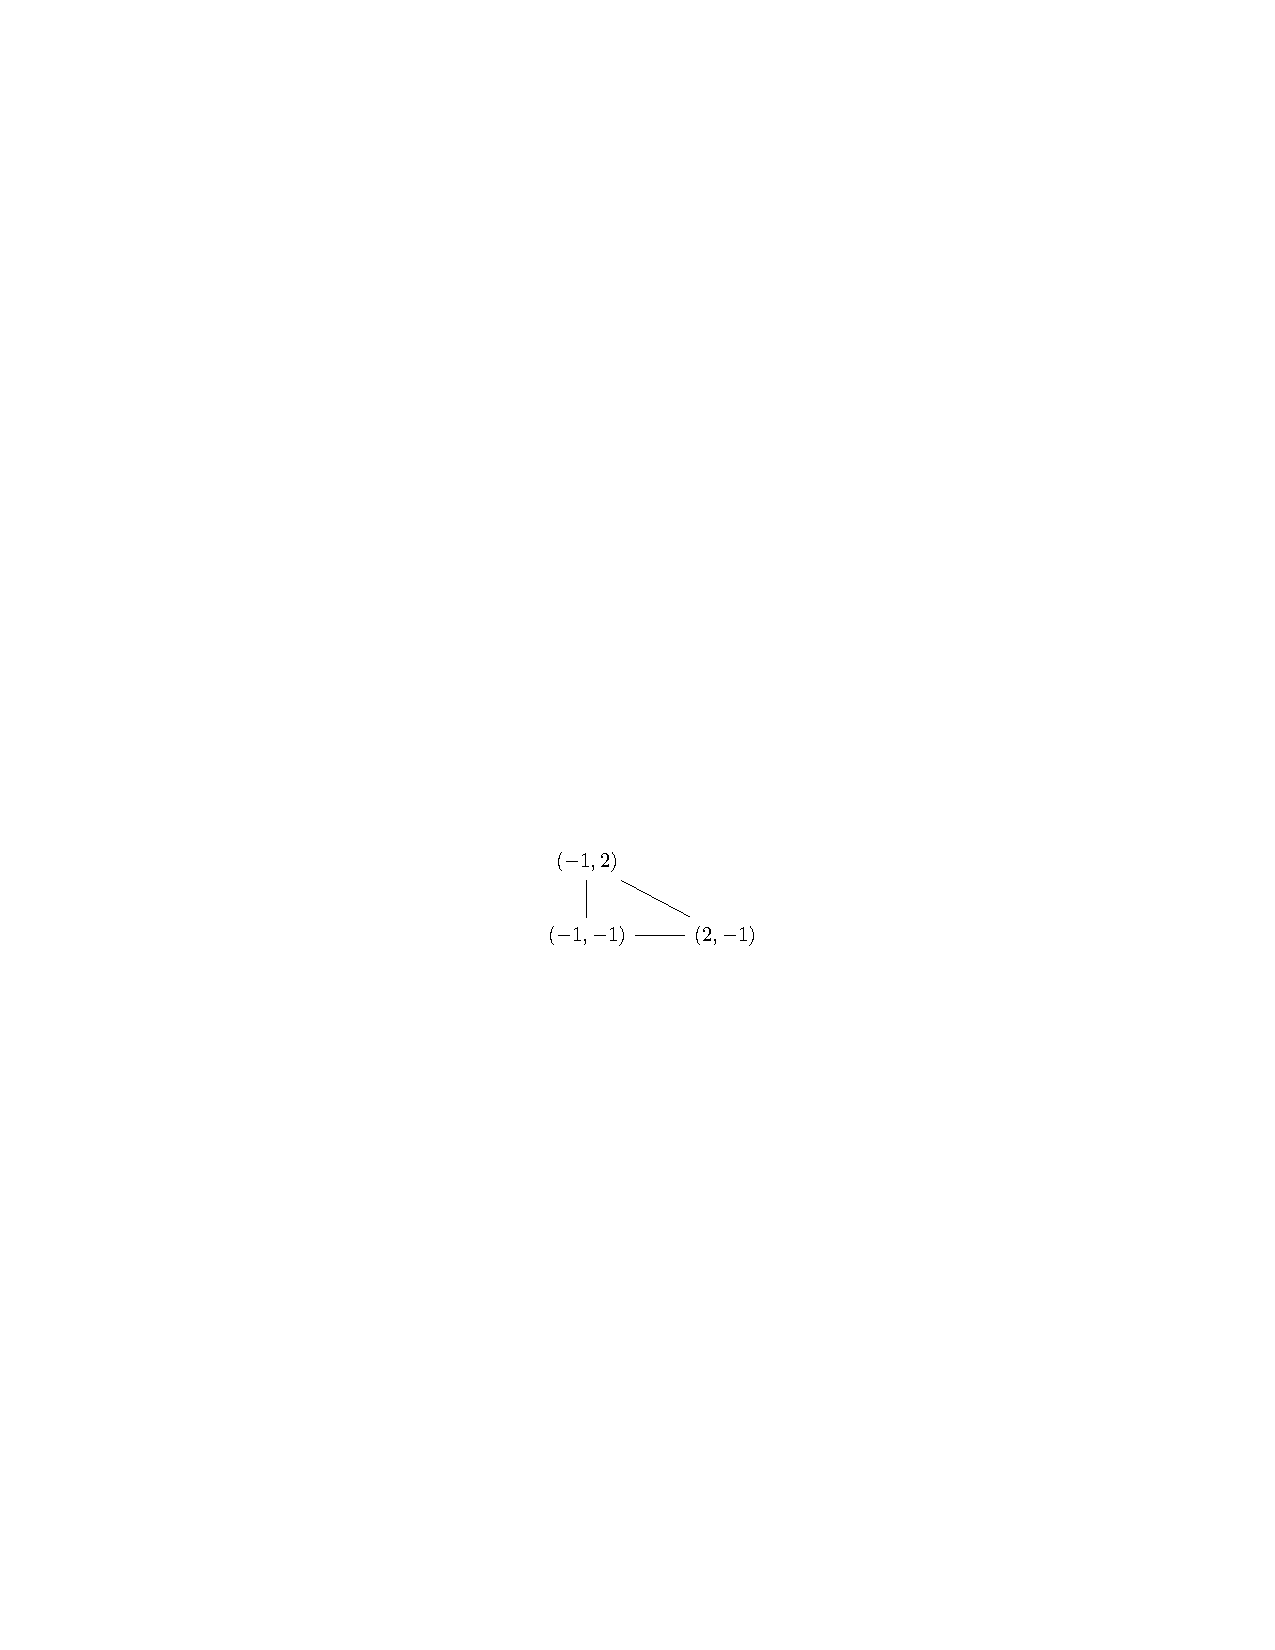
\includegraphics[width=0.2584\linewidth]{images/diagram-5-1.pdf}}}.}
则其对偶为
\Eq{5.2}{\Xi^\circ=\vcenter{\hbox{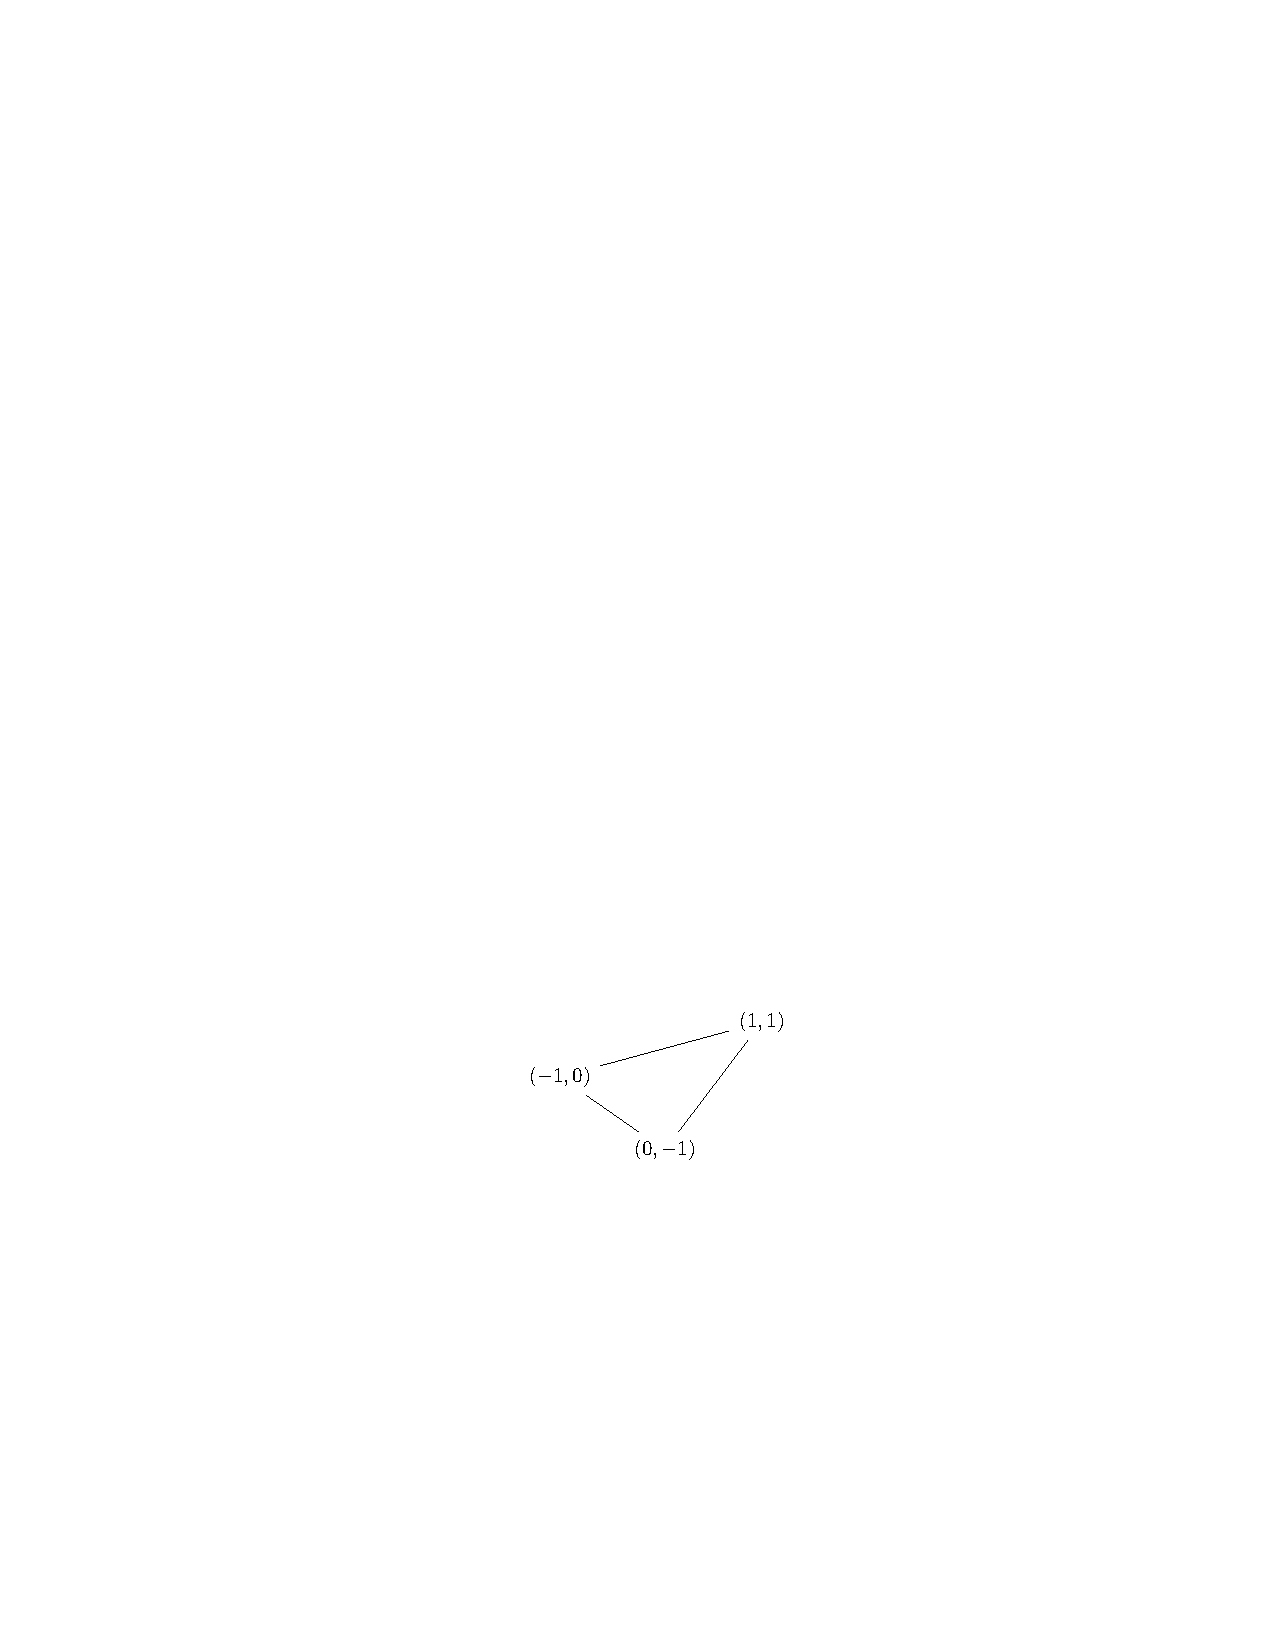
\includegraphics[width=0.3165\linewidth]{images/diagram-5-2.pdf}}}.}
二者都只有一个内部格点。
\end{example}
\examnum{2}\begin{example}\label{ex:5.2}
以原点为中心、边长为 $2$ 的正方形，其对偶可由它旋转 $45^\circ$ 并适当缩放得到。
\end{example}
二维中只有16个反身多胞体，见图~\ref{fig:5.1}。三维中有 $4319$ 个，四维中有 $473800776$ 个。人们说弦理论有许多不同的模型，就是由此而来。
\begin{Counterexample}{3}\label{counterex:3}
取 $(-1,-1),(-1,0),(1,0),(0,2)$ 的凸包，则它不是反身多胞体。
\end{Counterexample}
\SourcePage{82}
\OriginalFigure{fig-5-1.pdf}{0.5093}{二维的16个反身多胞体。原图来自文献~\cite{ref1}。}{fig:5.1}
\subsection{Fano 环面簇}
\thmnum{definition}{2}\begin{definition}\label{def:5.2}
若射影簇 $X$ 具有 Gorenstein 奇点，且反典范丛 $-K_X$ 丰，则称 $X$ 为 Fano 簇。对于此处考虑的正规 Cohen–Macaulay 环面簇，Gorenstein 条件等价于 $K_X$ 为 Cartier 除子，也等价于对偶化层为线丛。
\end{definition}
\thmnum{proposition}{1}\begin{proposition}\label{prop:5.1}
完备环面簇 $X$ 为 Fano 簇，当且仅当 $X\simeq X(\Sigma_\Xi)$，其中 $\Xi$ 反身。
\end{proposition}
\begin{proof}
令 $\Sigma$ 为 $N_{\RR}$ 中的扇。仿射坐标图 $U=\Spec k[\sigma^\vee\cap M]$ 的典范除子为 $K_U=-\sum_iD_i$，其中 $D_i$ 为环面素除子。全纯体积形式 $z_1^{-1}dz_1\wedge\cdots\wedge z_d^{-1}dz_d$ 沿每个环面除子都有一阶极点。

$K_U$ 为 Cartier 除子，当且仅当存在 $m_\sigma\in M$，使每条射线的本原生成向量 $v_i$ 都满足 $\langle m_\sigma,v_i\rangle=1$。把这一条件译成多胞体语言：$\Xi$ 是各 $m_\sigma$ 的凸包，而上述条件正是其侧面到原点的整距离为 $1$。
\end{proof}
\subsection{光滑情形中的 Calabi–Yau 超曲面}
设 $X$ 为光滑 Fano 簇，且 $\Gamma(X,-K_X)\ne0$。当反典范线性系无基点时，对一般截面 $s$，由 Bertini 定理，$Z(s)\subset X$ 光滑。伴随公式给出
\Eq{5.3}{K_{Z(s)}=(-K_X+K_X)|_{Z(s)}=0.}
问题在于，光滑 Fano 环面簇只有很少的几种。
\subsection{部分消解奇点}
记 $\Sigma_\Xi$ 为在 $\Xi^\circ$ 的各个面上取锥得到的扇。
\thmnum{definition}{3}\begin{definition}\label{def:5.3}
$\Sigma_\Xi$ 的一个极大、射影、保典范、部分细分，简称 MPCP 细分，是扇 $\Sigma$，满足：
\begin{itemize}
\item $\Sigma$ 是 $\Sigma_\Xi$ 的细分；
\item $\Sigma$ 单纯且射影；
\SourcePage{83}
\item 其射线的本原生成向量集合为
\Eq{5.4}{\Sigma(1)=\Xi^\circ\cap(N\setminus\{0\})=\partial\Xi^\circ\cap N.}
\end{itemize}
也就是说，要对 $\Xi^\circ$ 的每个面作使用全部边界格点的正则三角剖分。
\end{definition}
\begin{Note}{5.1}当 $d\ge3$ 时，$\Sigma$ 未必唯一，因为可能有许多不同的细分。\end{Note}
\thmnum{proposition}{2}\begin{proposition}\label{prop:5.2}
若 $\Sigma$ 是 MPCP 细分，则：
\begin{enumerate}[label=(\roman*)]
\item $X_\Sigma$ 是 Gorenstein 轨形；\footnote{在余维不超过3的点处光滑，但一般并非处处光滑。}
\item $\Xi$ 为与 $-K_{X_\Sigma}$ 关联的多胞体；
\item 诱导映射 $f:X_\Sigma\to X(\Sigma_\Xi)$ 保典范，即典范丛的拉回仍为典范丛：$K_{X_\Sigma}=f^*K_{X(\Sigma_\Xi)}$；
\item $-K_{X_\Sigma}$ 半丰，即由整体截面生成，而且是大的。\footnote{此处等价于 $(-K_{X_\Sigma})^d>0$。}
\end{enumerate}
\end{proposition}
\subsection{Batyrev 超曲面镜像}
设 $\Xi,\Xi^\circ$ 为一对反身多胞体，$\Sigma,\check\Sigma$ 分别为 $\Sigma_\Xi,\Sigma_{\Xi^\circ}$ 的 MPCP 细分。它们给出镜像对偶的族。对一般截面 $s\in\Gamma(X_\Sigma,-K_{X_\Sigma})$，构造
\Eq{5.5}{Z(s)\subset X_\Sigma.}
类似地，对 $\check s\in\Gamma(X_{\check\Sigma},-K_{X_{\check\Sigma}})$，构造
\Eq{5.6}{Z(\check s)\subset X_{\check\Sigma}.}
这些就是镜像对。注意，$\Gamma(X,-K_X)=\operatorname{Map}(\Xi\cap M,k)$。
\Lecture{23}{2019年11月19日}
\subsection{镜像定理}
\thmnum{theorem}{3}\begin{theorem}\label{thm:5.3}
若 $X$ 与 $\check X$ 均为光滑 Calabi–Yau 簇，则 $h^{1,1}(X)=h^{n-1,1}(\check X)$。
\end{theorem}
\begin{proof}见文献~\cite{ref6} 的定理4.15，或文献~\cite{ref2}。\end{proof}
\thmnum{theorem}{4}\begin{theorem}[Batyrev]\label{thm:5.4}
对于轨形奇点，存在 Hodge 数 $h^{p,q}$ 的“弦论”精化，满足
\Eq{5.7}{h^{p,q}_{\mathrm{st}}(X)=h^{n-p,q}_{\mathrm{st}}(\check X).}
\end{theorem}
这与动机积分有关。另外，Gromov–Witten 理论与镜像侧的 Hodge 结构变分相对应。
\thmnum{theorem}{5}\begin{theorem}\label{thm:5.5}
$\mathrm{GW}_{g=0}(X)=\mathrm{VHS}(\check X)$。
\end{theorem}
\begin{proof}见文献~\cite{ref5,ref12,ref22}。\end{proof}
还存在由 Batyrev–Borisov 给出的环面完全交推广。接下来的目标，是作出更内蕴的构造，以适用于更一般的情形；这正是文献~\cite{ref15,ref17} 中正在开展的研究。
\examnum{3}\begin{example}\label{ex:5.3}
考虑图~\ref{fig:5.2} 中的多胞体，按图右侧给顶点及格点标上单项式。这样便在 $\PP^2\times\mathbb A_t^1$ 中得到退化族
\Eq{5.8}{xyz+t^2(x^2y+xy^2+y^2z+yz^2+x^2z+xz^2)+t^3(x^3+y^3+z^3)=0.}
对一般非零 $t$，它是 Calabi–Yau 超曲面，即椭圆曲线；$t=0$ 时，$xyz=0$ 是三个超平面 $\PP^1$ 的并。
\end{example}
\SourcePage{84}
\OriginalFigure{fig-5-2.pdf}{0.5328}{多胞体及其唯一的 MPCP 细分；标注的数值给出一个分段线性函数。}{fig:5.2}
\OriginalFigure{fig-5-3.pdf}{0.8535}{从 $\Omega$ 出发构造族 $\mathcal X$。}{fig:5.3}
考虑 $\mathcal X\to S$，在变形理论中 $S$ 可以是某个离散赋值环的谱；实际上也可以取局部环或完备局部环的谱。我们希望零点上的纤维 $X_0$ 是若干环面簇的并，即把环面簇沿余维一分层作纤维余积粘合起来。
\section{Mumford 型环面退化}
\subsection{构造}
设 $\Omega\subset N_{\RR}$ 凸且闭。取有理多面体分解 $\mathscr P=\{\sigma\}$，使
\Eq{5.9}{\Omega=\bigcup_{\sigma\in\mathscr P}\sigma,}
此分解局部有限，且各胞腔沿共同的面相交。由此得到扇
\Eq{5.10}{\Sigma_{\mathscr P}=\{C(\sigma)\subset N_{\RR}\oplus\RR:\sigma\in\mathscr P\}\cup\{\text{这些锥的所有面}\}.}
其想法是把 $\Omega$ 放在高度一处，再像图~\ref{fig:5.3} 那样取锥。高度投影诱导 $\pi:X(\Sigma_{\mathscr P})\to\mathbb A^1$。
\thmnum{proposition}{6}\begin{proposition}\label{prop:5.6}
\begin{enumerate}[label=(\alph*)]
\item $\pi^{-1}(\mathbb A^1\setminus\{0\})\simeq(\mathbb A^1\setminus\{0\})\times X(\Sigma_{\mathscr P}\cap(N_{\RR}\times\{0\}))$，总维数为 $d+1$。
\item
\Eq{5.11}{\pi^{-1}(0)=\bigcup_{v\text{ 为 }\mathscr P\text{ 的顶点}}\underbrace{X((\Sigma_{\mathscr P})_v)}_{D_v}.}
\item
\Eq{5.12}{\operatorname{mult}_{D_v}(\pi^{-1}(0))=\min\{d\in\NN\setminus\{0\}:dv\in N\}.}
\end{enumerate}
\end{proposition}
\SourcePage{85}
\begin{proof}
(a) $\pi^{-1}(\mathbb A^1\setminus\{0\})$ 对应于 $N\oplus\ZZ$ 中的扇 $\{C(\sigma)\cap(N_{\RR}\times\{0\})\}$。
(b) $\pi^{-1}(0)$ 是那些映到 $\mathbb A^1$ 原点的环面素除子 $D_w$ 的并，其对应射线 $w$ 在高度投影下非零。
(c) 射线由本原格向量 $(n,d)$ 生成，其中 $v=n/d$，$d>0$ 最小。由单项式的阶数公式，
\Eq{5.13}{\operatorname{ord}_{D_w}\pi^*(t)=d.}
\end{proof}
在图~\ref{fig:5.3} 的例子中，$t\ne0$ 时 $\pi^{-1}(t)=\PP^2$；$t=0$ 时，
\Eq{5.14}{\pi^{-1}(0)=\bigcup_{i=1}^3X\left(\vcenter{\hbox{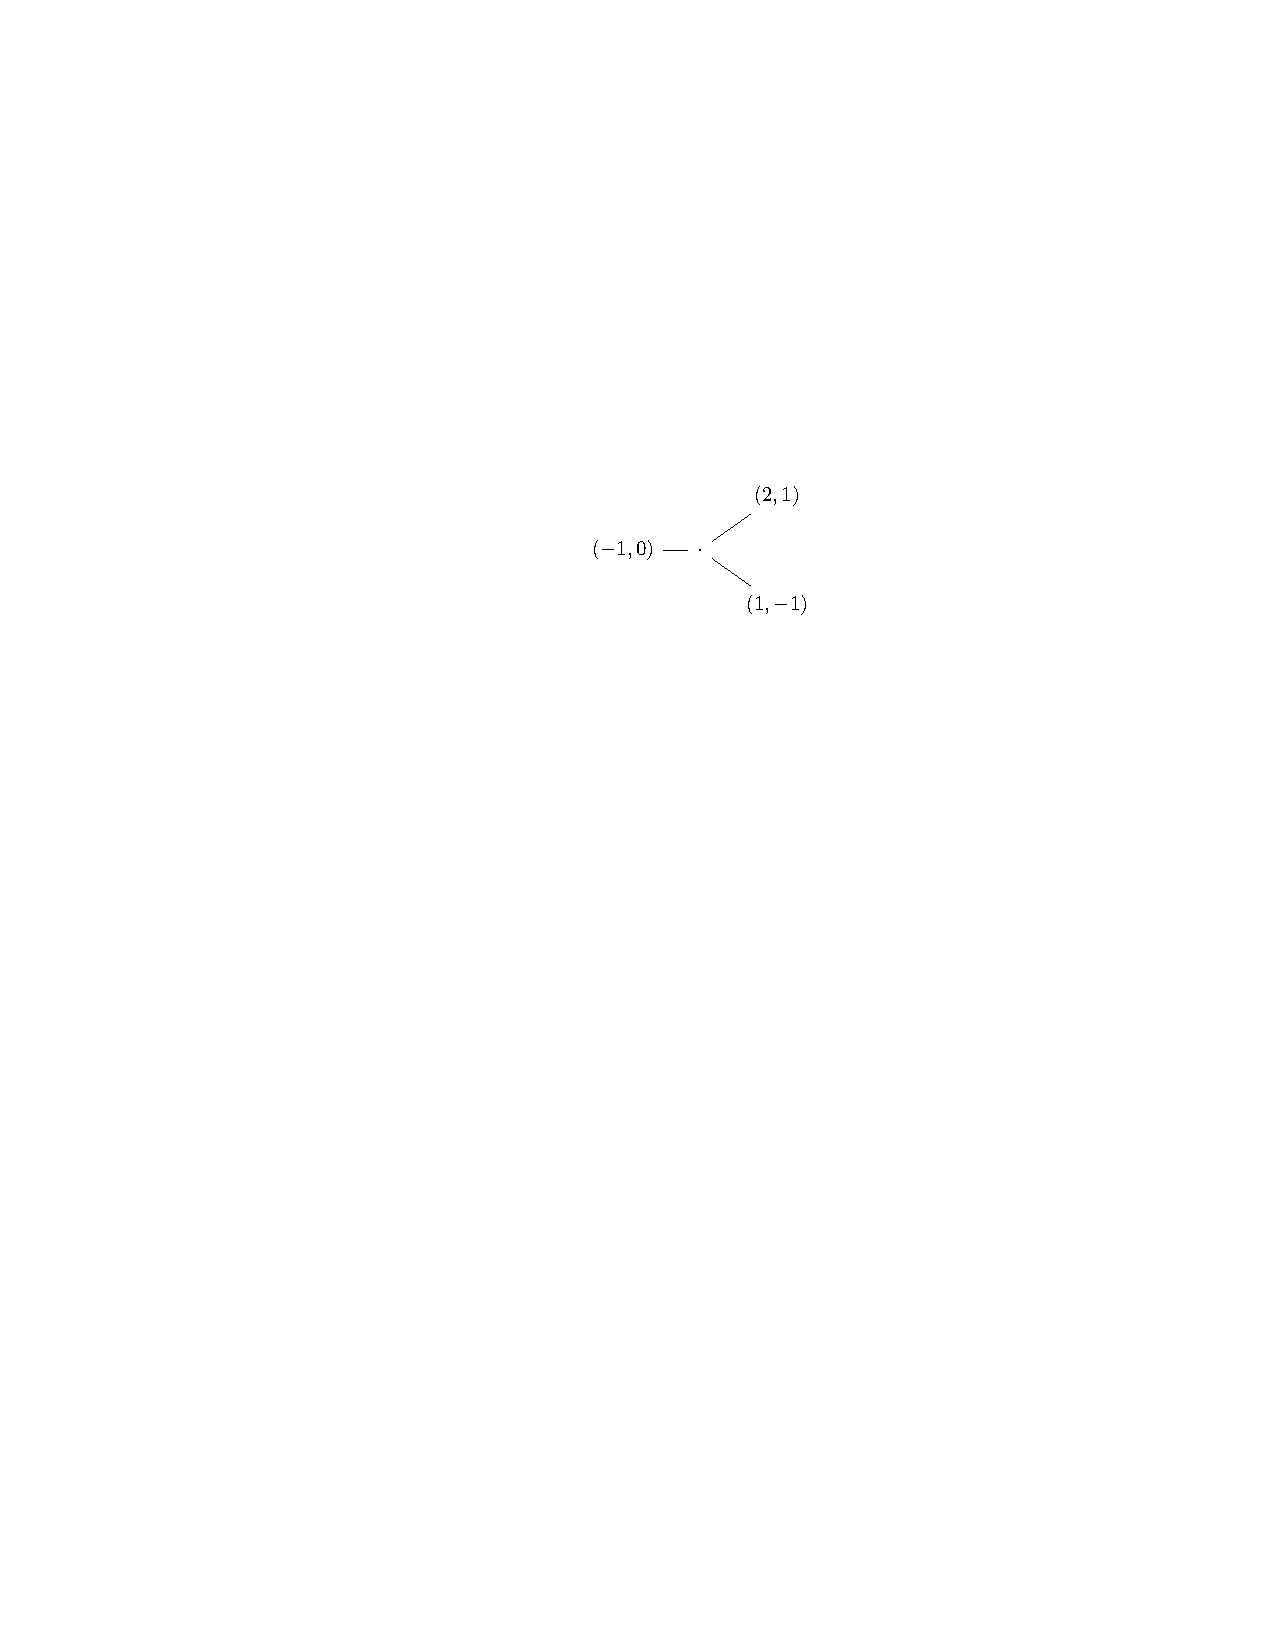
\includegraphics[width=0.2677\linewidth]{images/diagram-5-14.pdf}}}\right).}
注意，每个不可约分支都满足
\Eq{5.15}{\PP^2\xrightarrow{/\,(\ZZ/3)}D_v\simeq\PP(1,1,3).}
\subsection{多胞体图景}
镜像对称需要带极化的版本。对有理多面体 $\Xi\subset M_{\RR}$，记其有理多面体分解为 $\check{\mathscr P}$。若细分正则，则在适当放大后，存在整分段仿射严格凸函数 $\check\varphi:\Xi\to\RR$。其图像为 $\Gamma_{\check\varphi}\subset M_{\RR}\times\RR$，上方凸包为
\Eq{5.16}{B_{\check\varphi}=\Gamma_{\check\varphi}+(0\oplus\RR_{\ge0})=\{(m,h)\in\Xi\times\RR:h\ge\check\varphi(m)\}.}
由此得到带极化的 Mumford 退化
\Eq{5.17}{X(\Sigma_{B_{\check\varphi}}),}
其中，
\Eq{5.18}{X(\Sigma_{B_{\check\varphi}})\simeq\operatorname{Proj}k[C(B_{\check\varphi})\cap(M\oplus\ZZ\oplus\ZZ)].}
\subsection{Mumford 退化的镜像对称}
其思想是如下的一一对应：
\Eq{5.19}{\begin{aligned}(B=|\mathscr P|,\mathscr P,\varphi)&\longleftrightarrow(\check B=|\check{\mathscr P}|,\check{\mathscr P},\check\varphi),\\\text{分段仿射函数}&\longmapsto\check\sigma=\text{$\varphi|_{\Sigma_\sigma}$ 的 Newton 多面体},\quad\sigma\in\mathscr P,\\(\Sigma_{\mathscr P},\psi)&\longleftrightarrow(\Xi,\check\psi),\end{aligned}}
其中 $\psi$ 为分段线性函数。
\examnum{4}\begin{example}\label{ex:5.4}
图~\ref{fig:5.4} 的 $\mathscr P$ 给出 $\PP^2$ 的一个环面退化；图中还画出了对应的 $\check{\mathscr P}$。
\end{example}
\Lecture{24}{2019年11月21日}
\SourcePage{86}
\OriginalFigure{fig-5-4.pdf}{0.9579}{一个 $\mathscr P$ 与 $\check{\mathscr P}$ 的例子。}{fig:5.4}
\subsection{环面退化}
于是有
\Eq{5.20}{\begin{tikzcd}X_0\arrow[r,hook]\arrow[d]\&(\mathcal X,\mathcal L)\arrow[d,"{\pi}"]\\0\arrow[r,hook]\&S_t=\Spec(\text{离散赋值环}),\end{tikzcd}}
其中希望 $X_0$ 是射影环面簇的并，且 $\mathcal L|_{P(\sigma)}=\OO_{P(\sigma)}(1)$。相应数据为 $(B=\bigcup\sigma,\mathscr P=\{\sigma\},\varphi)$，其中 $B$ 是带边界流形，$\dim_{\RR} B=\dim X=d$，$\varphi$ 为极化函数。这是扇的图景；$\varphi$ 对应于 $\pi$ 在余维一处的环面模型。

还存在等价的多面体构造。\Term{lisanlegendre}{离散 Legendre 变换}就是数据 $(B,\mathscr P,\varphi)$ 的镜像对偶，产生 $(\check B,\check{\mathscr P},\check\varphi)$。
\section{走向 Gross–Siebert 型环面退化}
\subsection{Dwork 族与\texorpdfstring{$A_1$}{A₁}奇点}
考虑
\Eq{5.21}{\mathcal X=Z\left(t\sum_{i=0}^3z_i^4+\prod_{i=0}^3z_i\right)\subset\PP^3\times\mathbb A^1,}
并投影到 $\mathbb A^1$。这是课程开头五次超曲面族的低一维对应，给出 K3 曲面的退化。$X_0=\pi^{-1}(0)$ 是四个 $\PP^2$ 的并，各个 $\PP^2$ 由极大胞腔对应的 $P(\sigma)$ 给出。总空间 $\mathcal X$ 在 $X_0$ 的奇异轨迹上有 $6\cdot4=24$ 个三维 $A_1$ 奇点；这个轨迹由6条 $\PP^1$ 组成。

在 $z_0,z_1\ne0$ 处，以 $z_0=1$ 去齐次化，得到局部方程
\Eq{5.22}{z_2z_3=-t\,\frac{1+z_1^4+z_2^4+z_3^4}{z_1}.}
在奇点附近作解析坐标变换后，它同构于 $uv=wt$，即一个 $A_1$ 奇点。模 $t^{k+1}$ 后，
\Eq{5.23}{\mathcal X\bmod t^{k+1}=\bigcup_{i=0}^3X_{\sigma_i}^k,}
其中 $X_{\sigma_i}^0=P(\sigma_i)$。这些对象本质上是 $X_{\sigma_i}\subset\mathcal X$ 的 $k$ 阶邻域。观察到，各个局部模型
\SourcePage{87}
完全由 $(B,\mathscr P,\varphi)$ 决定；只有更高余维处的识别不是环面的，即粘合并非环面粘合。
\subsection{关键例子：一个\texorpdfstring{$A_1$}{A₁}奇点}
考虑两个胞腔 $\sigma_1,\sigma_2$，它们都是半平面，交于实直线 $\rho$。把交集上的坐标记为 $w$，$\sigma_1$、$\sigma_2$ 的横向坐标分别记为 $u,v$。我们希望交集上的 $w=-1$ 处出现一个 $A_1$ 奇点。因此取
\Eq{5.24}{uv=\underbrace{(1+w)}_{f_\rho}\,t\pmod{t^{k+1}}.}
要粘合的环面模型为
\Eq{5.25}{R_{\sigma_1}=\CC[u,v,w^{\pm1},t]/(uv-t,t^{k+1},v^{k+1}),}
\Eq{5.26}{R_{\sigma_2}=\CC[u,v,w^{\pm1},t]/(uv-t,t^{k+1},u^{k+1}).}
相交处的模型为 $X_\rho^k=\Spec R_{\rho,\sigma_i}$。在 $f_\rho$ 可逆的开集上，粘合图为
\Eq{5.27}{\begin{gathered}R_{\sigma_1}[f_\rho^{-1}]\longrightarrow R_{\rho,\sigma_1}=(R_{\sigma_1}/(u^{k+1}))[f_\rho^{-1}],\\R_{\sigma_2}[f_\rho^{-1}]\longrightarrow R_{\rho,\sigma_2}=(R_{\sigma_2}/(v^{k+1}))[f_\rho^{-1}],\\R_{\rho,\sigma_1}\xrightarrow{\sim}R_{\rho,\sigma_2},\qquad u\longmapsto f_\rho u,\quad v\longmapsto f_\rho^{-1}v.\end{gathered}}
反向识别把 $u$ 映为 $f_\rho^{-1}u$，$v$ 映为 $f_\rho v$。于是取纤维积得到
\Eq{5.28}{\begin{aligned}R_{\sigma_1}[f_\rho^{-1}]\times_{R_{\rho,\sigma_i}}R_{\sigma_2}[f_\rho^{-1}]&\simeq\left(\frac{\CC[u,v,w^{\pm1},t]}{uv-(1+w)t,\ t^{k+1}}\right)_{f_\rho},\\u&\longmapsto(u,f_\rho u),\\v&\longmapsto(f_\rho v,v),\\w&\longmapsto(w,w).\end{aligned}}

因此，在余维二轨迹之外，我们有由 $(B,\mathscr P,\varphi)$ 给出的两类环面模型。对于极大胞腔 $\sigma$，
\Eq{5.29}{R_\sigma^k=A_k[\Lambda_\sigma],}
其中 $A_k=\CC[t]/(t^{k+1})$，$\Lambda_\sigma\simeq\ZZ^d$ 是 $\sigma$ 所在的整切格。可把其中的元素理解为 $\sigma$ 上的整切向量。对于余维一胞腔 $\rho\in\mathscr P[d-1]$，
\Eq{5.30}{R_\rho^k=A_k[\Lambda_\rho][Z_+,Z_-]/(Z_+Z_--f_\rho t^{\kappa_\rho(\varphi)}),}
其中 $\kappa_\rho(\varphi)\in\NN\setminus\{0\}$ 是 $\varphi$ 沿 $\rho$ 的折角，$f_\rho\in A_k[\Lambda_\rho]$。这就是所谓数据位于一面壁上的含义。
\section{重构}
问题是如何从 $(B,\mathscr P,\varphi)$ 得到族 $\mathcal X\to S$。我们将把 $\Spec R_\sigma^k$ 与 $\Spec R_\rho^k$ 作纤维余积粘合，以构造 $\mathcal X$。具体的初始数据为
\Eq{5.31}{\left(B=\bigcup_{\sigma\in\mathscr P}\sigma,\ \mathscr P,\ \varphi,\ f_\rho\in A_k[\Lambda_\rho]\right).}
\SourcePage{88}
\subsection{不涉及散射的说明}
顶点 $v_1$ 处的扇结构为
\Eq{5.32}{\vcenter{\hbox{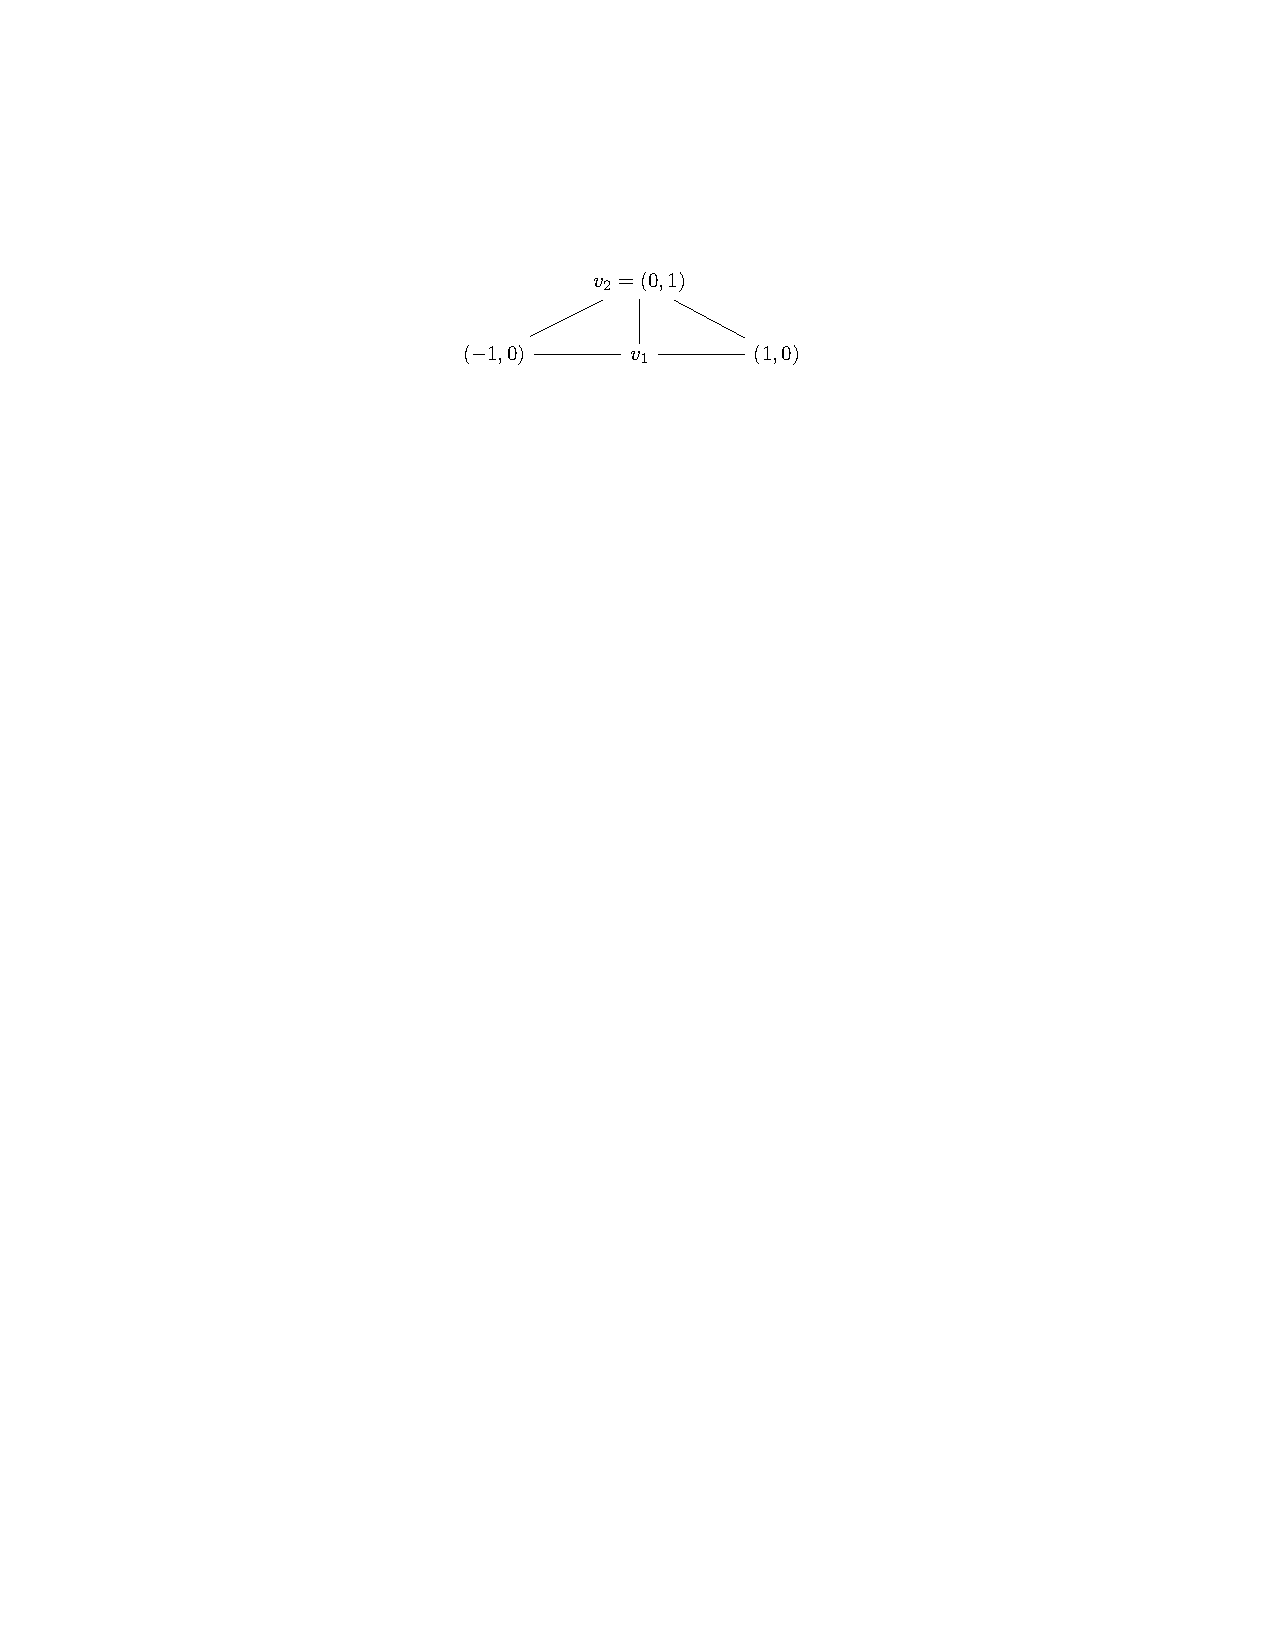
\includegraphics[width=0.4141\linewidth]{images/diagram-5-32.pdf}}}.}
顶点 $v_2$ 处的扇结构为
\Eq{5.33}{\vcenter{\hbox{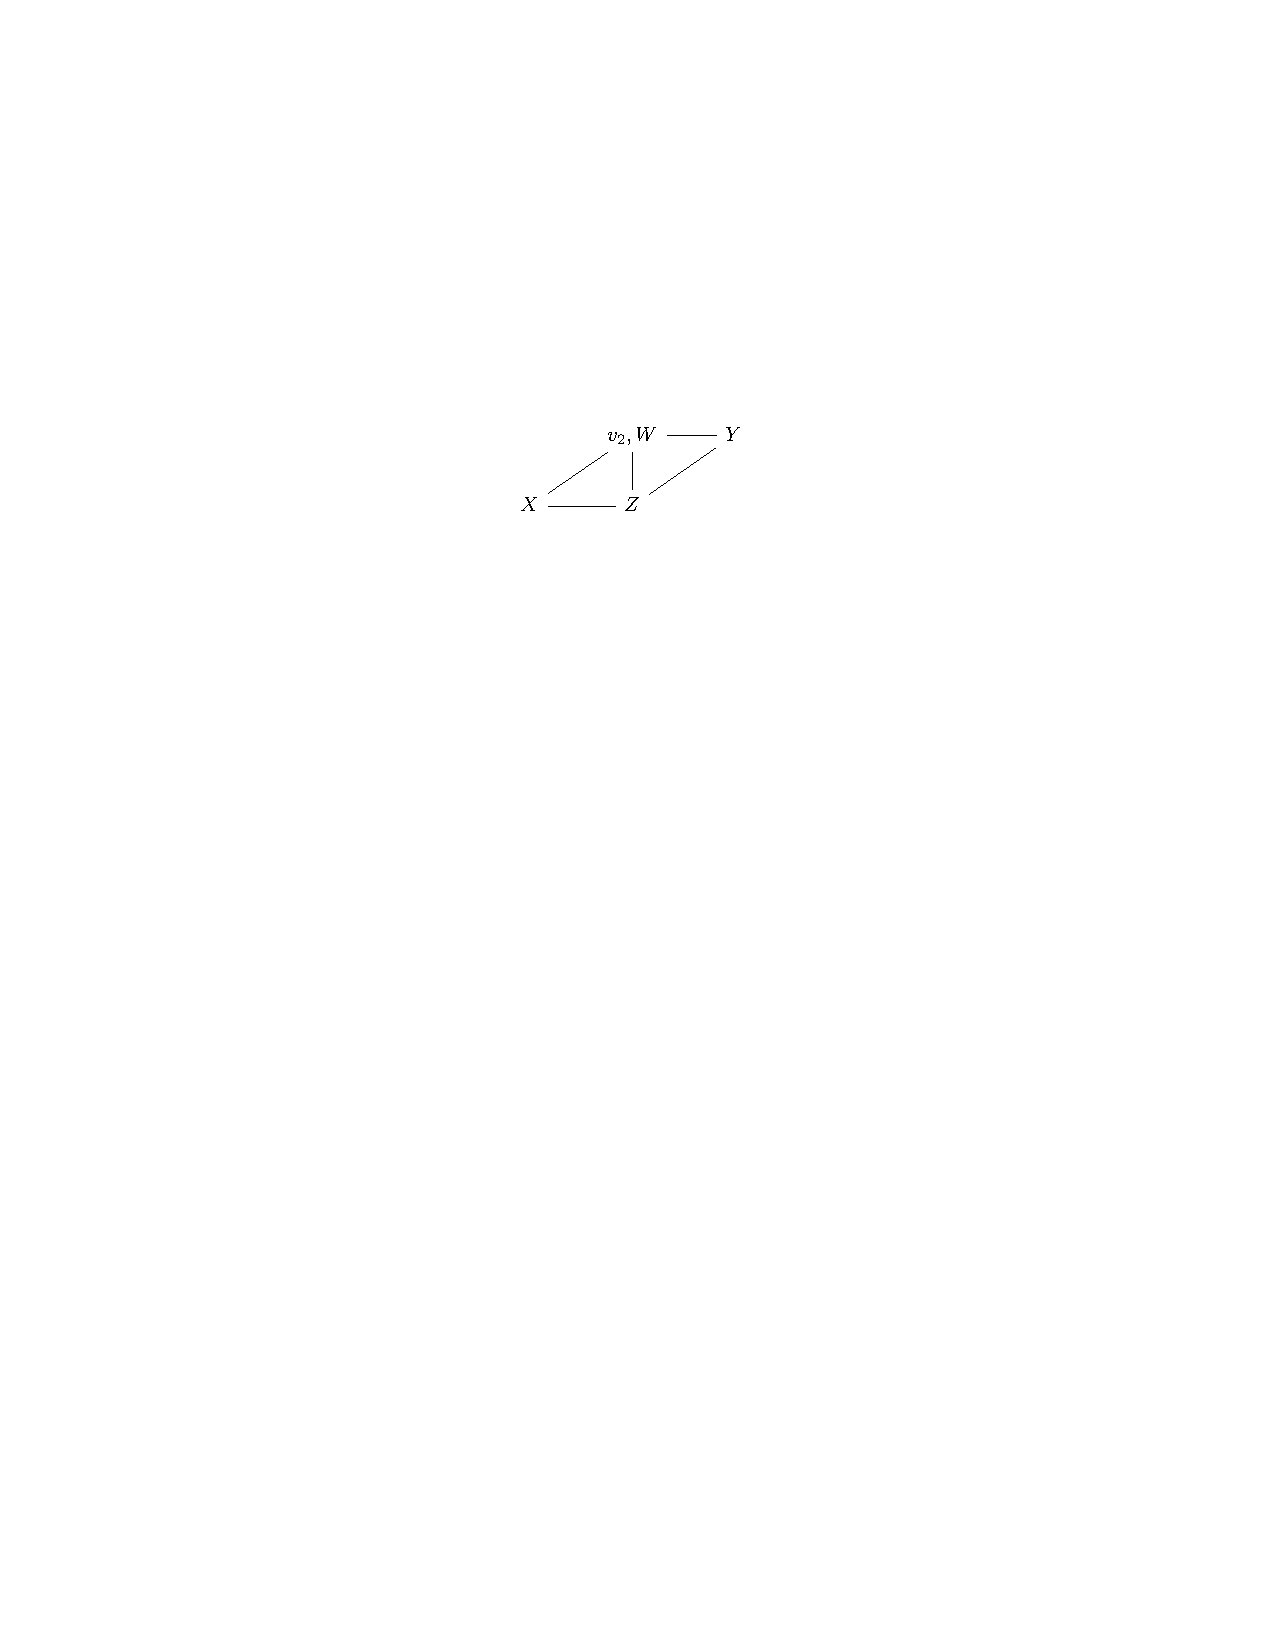
\includegraphics[width=0.2786\linewidth]{images/diagram-5-33.pdf}}}.}
这些结构给出不同的仿射结构。删去内部边上的一个点，就能处理这种差异。这里取
\Eq{5.34}{f_{\rho,v_1}=\alpha+w,}
其中 $\alpha\in\CC^\times$、$w=W/Z$。对 $R_{\rho,v_1}^k$，有
\Eq{5.35}{Z_+=y=Y/Z,}
\Eq{5.36}{Z_-=x=X/Z,}
以及方程
\Eq{5.37}{Z_+Z_-=(\alpha+w)t.}
齐次化得到
\Eq{5.38}{\frac YZ\frac XZ=\left(\alpha+\frac WZ\right)t.}
这给出一个非环面的二次曲线退化族。若采用 Mumford 型退化，则 $\alpha Z+W$ 会被单项式 $W$ 代替。

类似地，在 $R_{\rho,v_2}^k$ 的坐标中，令 $y=Y/W$、$x=X/W$、$z=Z/W$，有
\Eq{5.39}{Z_+=y=\frac YW,\qquad Z_-=xz^{-1}=\frac XW\frac WZ=\frac XZ.}
于是
\Eq{5.40}{Z_+Z_-=(z\alpha+1)t.}
齐次化后，
\Eq{5.41}{\frac YW\frac XZ=\left(\frac ZW\alpha+1\right)t,}
因此
\Eq{5.42}{XY=(Z\alpha+W)Zt.}
最终得到相容的模型
\Eq{5.43}{f_{\rho,v_1}=z^{m^\rho_{v_1,v_2}}f_{\rho,v_2},}
其中 $m^\rho_{v_1,v_2}\in\Lambda_\rho$。在本例中，$m^\rho_{v_1,v_2}=(0,1)$。将它加入初始数据，得到
\Eq{5.44}{(B,\mathscr P,\varphi,\{f_{\rho,v}\}).}
\SourcePage{89}
\subsubsection{传播}
考虑四个象限的副本粘合在一起：
\Eq{5.45}{\vcenter{\hbox{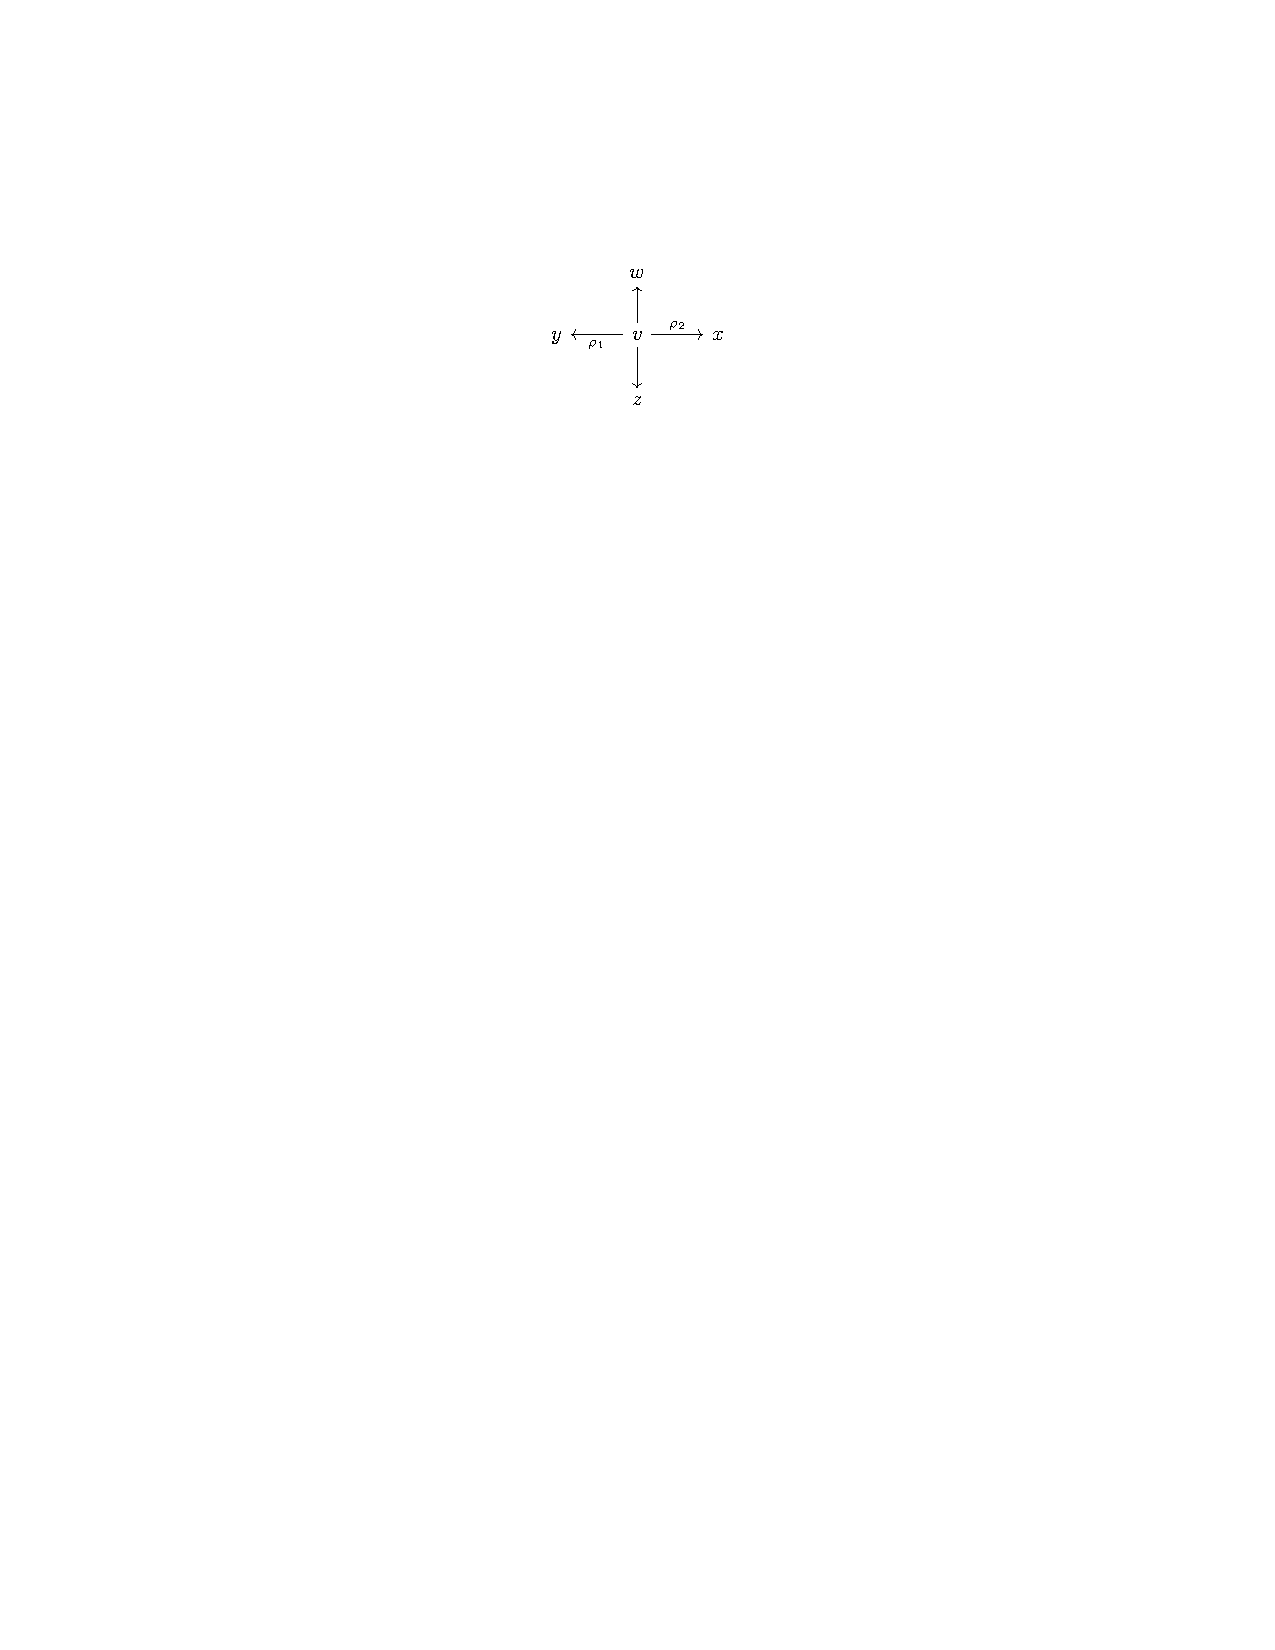
\includegraphics[width=0.2197\linewidth]{images/diagram-5-45.pdf}}}.}
顶点 $v$ 处的环面模型为
\Eq{5.46}{A_k[x,y,z,w]/(xy-t,zw-t).}
现在取 $f_{\rho_1}=1+y$。$R_{\rho_1}^k$ 的局部模型为 $zw=(1+y)t$。当 $x\ne0$ 时，$y=x^{-1}t$，所以必须有局部模型
\Eq{5.47}{zw=(1+x^{-1}t)t.}
这迫使我们令
\Eq{5.48}{f_{\rho_2}=1+x^{-1}t.}
可把这一过程理解为：每面壁都携带一个单项式的数据。
\subsubsection{离开余维一轨迹的壁}
\Eq{5.49}{\vcenter{\hbox{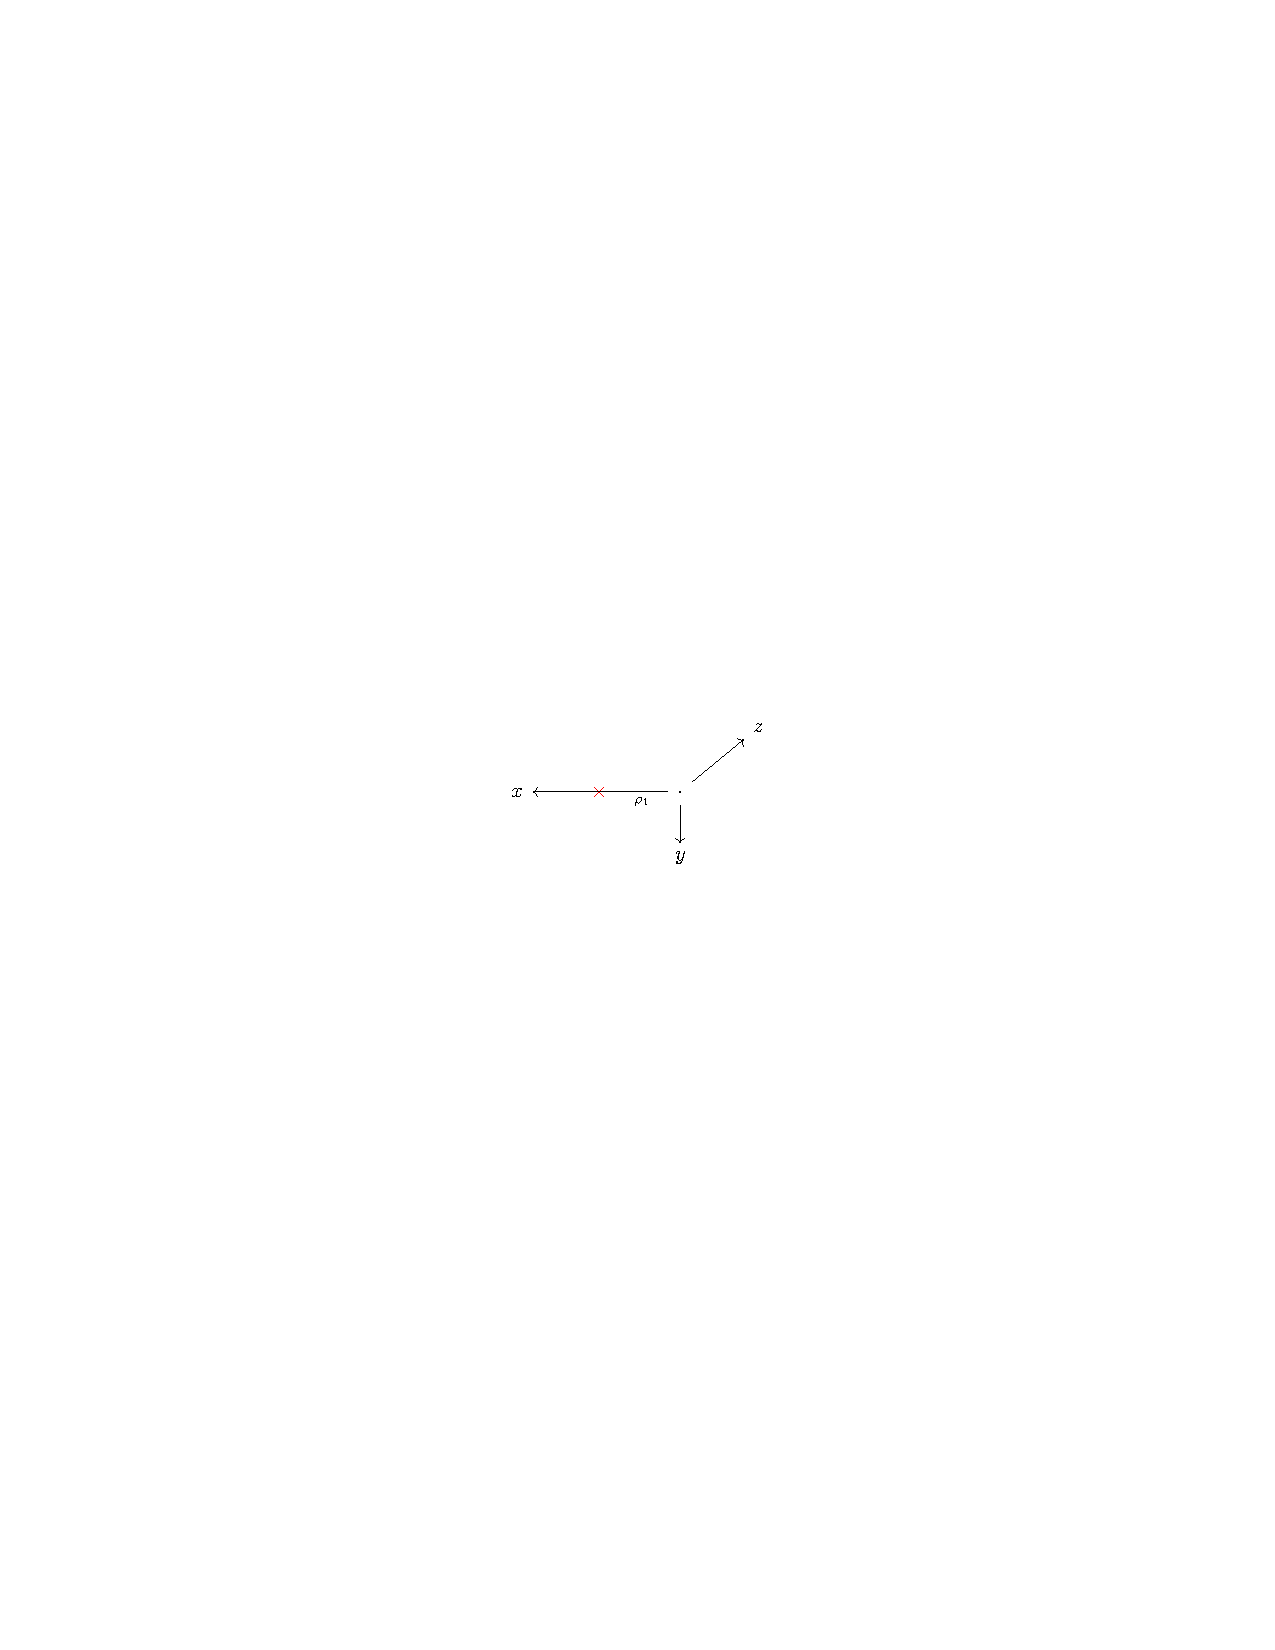
\includegraphics[width=0.3157\linewidth]{images/diagram-5-49.pdf}}}.}
环面模型为 $xyz=t$，且
\Eq{5.50}{f_{\rho_1}=1+x=1+(yz)^{-1}t.}
为了使它相容，取两个 $R_\sigma^k$ 的副本，并用一个非环面的“壁穿越”自同构 $\Phi$ 粘合。具体地，
\Eq{5.51}{\begin{aligned}y&\xmapsto{\Phi}(1+y^{-1}z^{-1}t)y,\\z&\xmapsto{\Phi}\underbrace{(1+y^{-1}z^{-1}t)^{-1}}_{\equiv1\pmod t}\,z.\end{aligned}}
\Lecture{25}{2019年11月26日}
\section{壁结构}
\subsection{壁}
固定 $k$，令 $A=\CC[t]/(t^{k+1})$；最终将令 $k\to\infty$。与往常一样，初始数据为
\Eq{5.52}{\left(B=\bigcup_{\sigma\in\mathscr P}\sigma,\ \mathscr P=\{\sigma\},\ \varphi\right),}
其中 $B$ 带有整仿射结构。奇异轨迹 $\Delta\subset B$ 的实余维为 $2$。
\thmnum{definition}{4}\begin{definition}\label{def:5.4}
$B$ 上的一面\Term{bi}{壁} $\mathfrak p$ 由以下数据组成：
\SourcePage{90}
\begin{itemize}
\item 有理多面体子集 $\mathfrak p\subseteq\sigma$，其中 $\dim\sigma=d$、$\dim\mathfrak p=d-1$，且 $\Int(\mathfrak p)\cap\Delta=\varnothing$；
\item 函数 $f_{\mathfrak p}=\sum_mc_mz^m$，其中 $m\in\Lambda_{\mathfrak p}\subset\Lambda_\sigma\simeq\ZZ^d$、$c_m\in A$。
\end{itemize}
\end{definition}
在余维零处，即 $\mathfrak p\cap\Int(\sigma)\ne\varnothing$ 时，有 $f_{\mathfrak p}=1+c_mz^m$，且 $c_m\equiv0\pmod t$。$m$ 给出传播方向；这种壁称为真壁。在余维一处，即 $\mathfrak p\subseteq\rho$、$\dim\rho=d-1$ 时，采用来自 $\rho$ 的函数 $f_{\mathfrak p}=f_\rho$，这种壁称为\Term{biban}{壁板}。对有限的 $k$，\Term{bijiegou}{壁结构} $\mathscr S$ 是壁的有限集合。
\subsection{壁穿越}
设 $(\mathfrak p,f_{\mathfrak p})$ 为余维零处的壁，$\mathfrak p\subset\sigma$。记
\Eq{5.53}{R_\sigma=A[\Lambda_\sigma]\simeq A[z_1^{\pm1},\ldots,z_d^{\pm1}].}
壁定义一个自同构
\Eq{5.54}{\Theta_{\mathfrak p}:R_\sigma\longrightarrow R_\sigma,}
其作用为
\Eq{5.55}{z^m\longmapsto f_{\mathfrak p}^{\langle n_{\mathfrak p},m\rangle}z^m,}
其中 $n_{\mathfrak p}\in\Lambda_\sigma^*$ 为按穿越方向选择的本原法向余向量，$n_{\mathfrak p}^\perp=\Lambda_{\mathfrak p}$。由于 $\Theta_{\mathfrak p}\equiv\id\pmod t$，它确实是自同构。
\examnum{5}\begin{example}\label{ex:5.5}
考虑如下壁：
\Eq{5.56}{\vcenter{\hbox{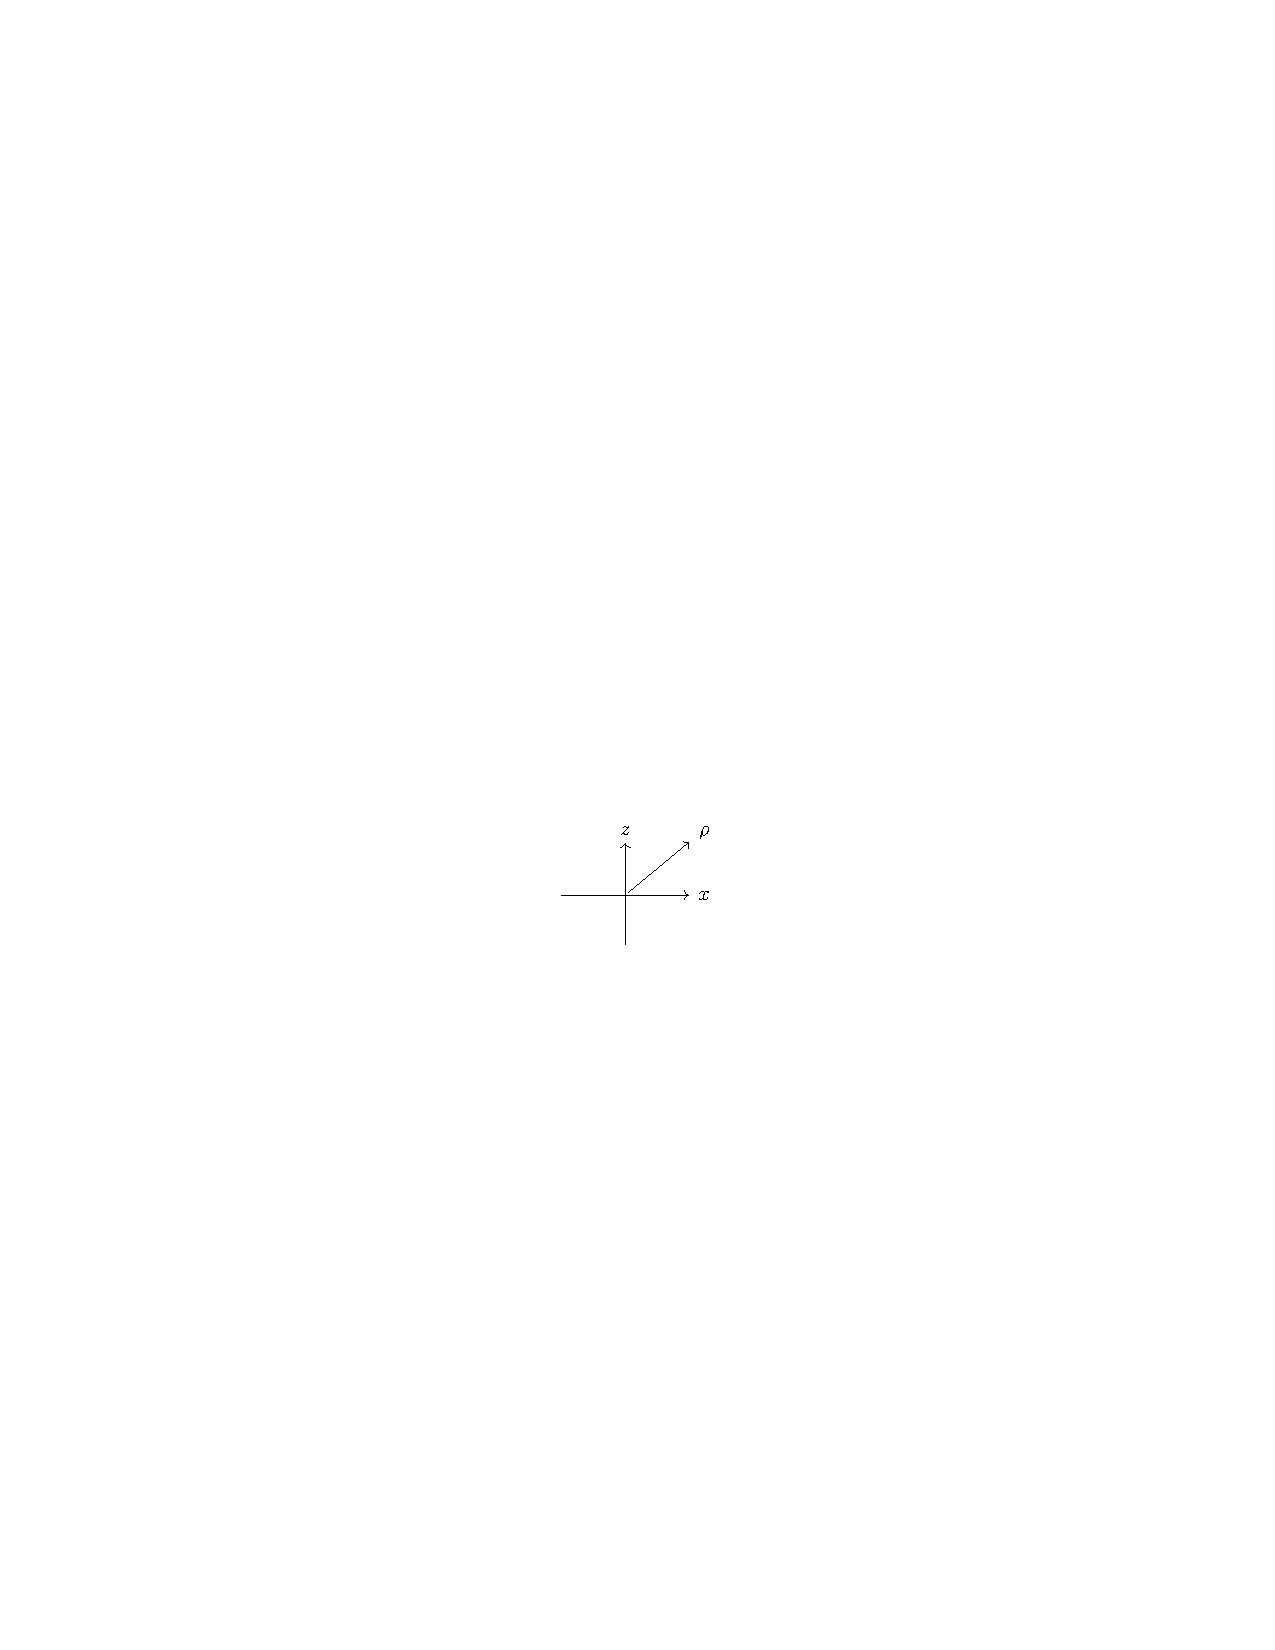
\includegraphics[width=0.1902\linewidth]{images/diagram-5-56.pdf}}}.}
从 $x$ 的方向向 $z$ 的方向穿过它。先取 $f_{\mathfrak p}=1+t^2x^{-1}z^{-1}$，则 $\Theta_{\mathfrak p}$ 映为
\Eq{5.57}{x\longmapsto(1+t^2x^{-1}z^{-1})x,\qquad z\longmapsto(1+t^2x^{-1}z^{-1})^{-1}z.}
\end{example}
\examnum{6}\begin{example}\label{ex:5.6}
传播中的壁沿余维二的多面体子集相交，这些子集称为\Term{jiehebu}{接合部}。采用下图的记号：
\Eq{5.58}{\vcenter{\hbox{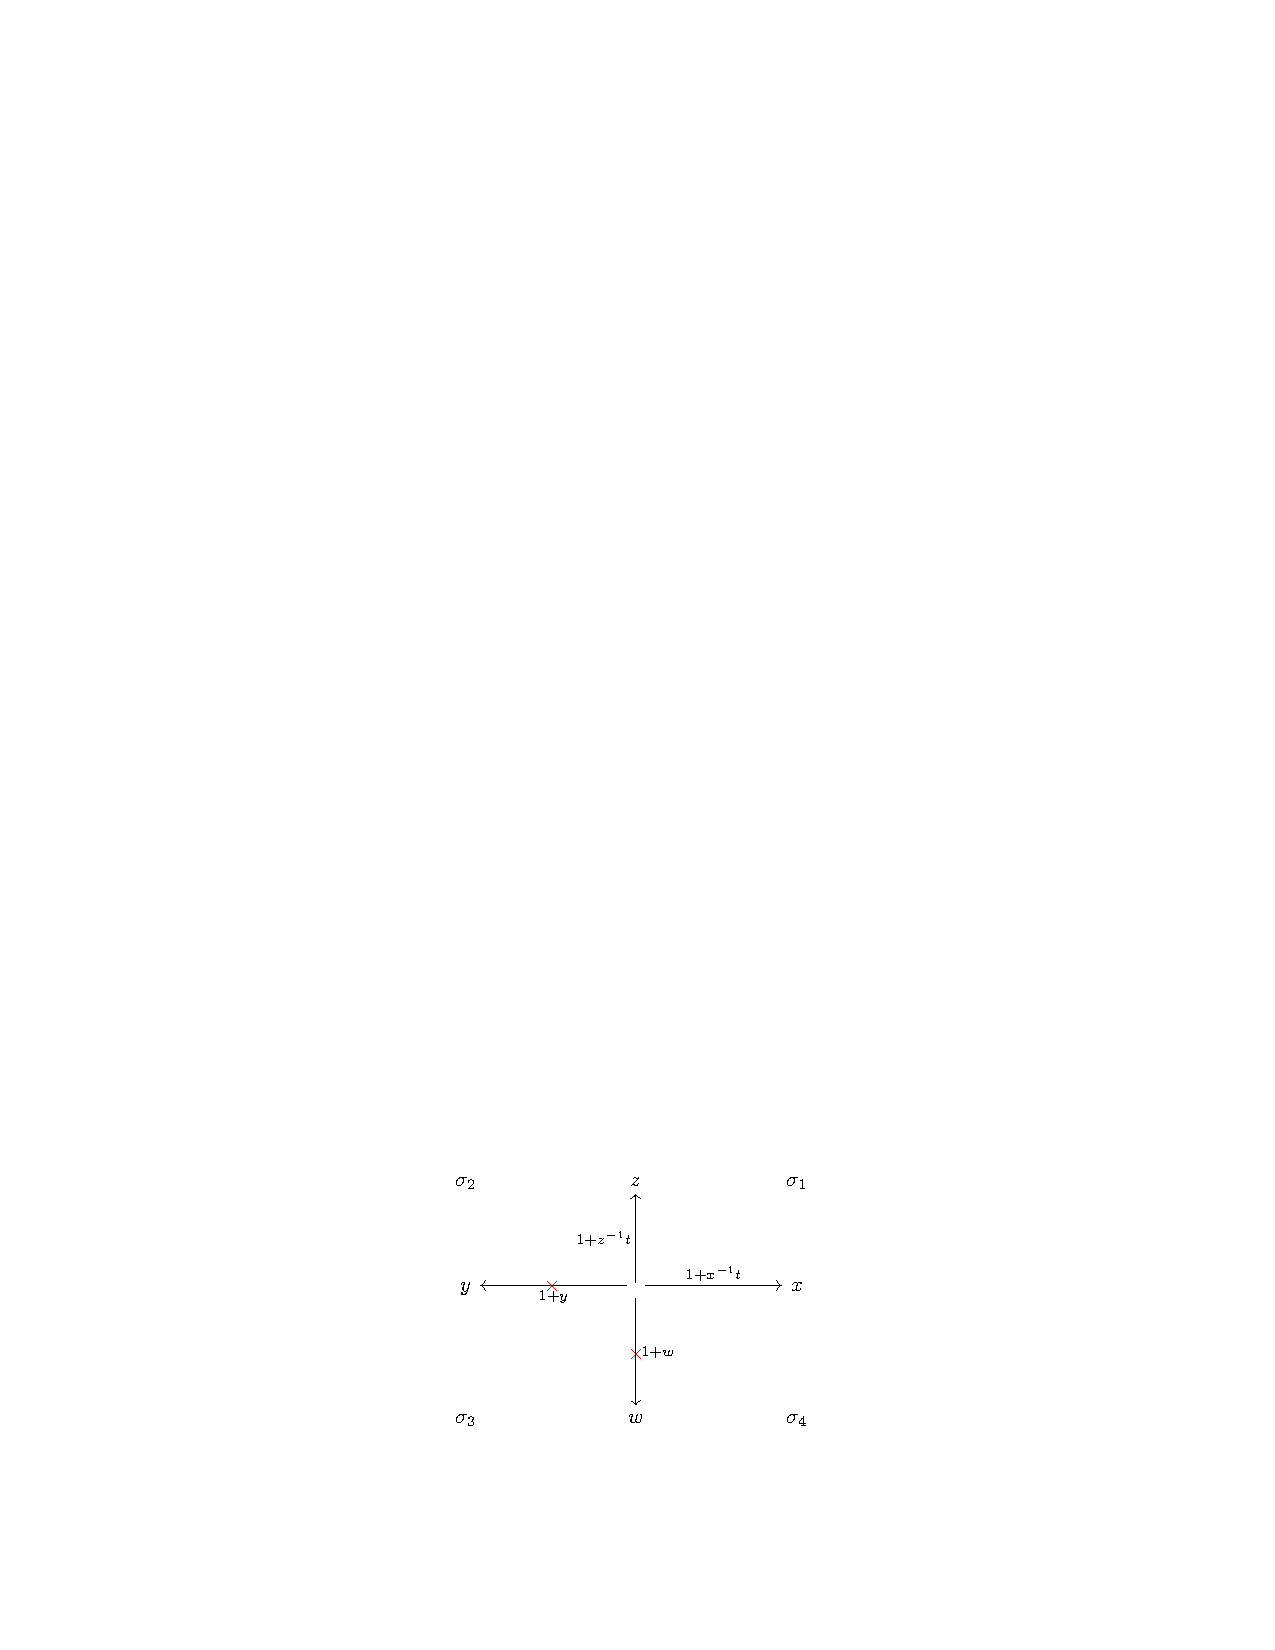
\includegraphics[width=0.4343\linewidth]{images/diagram-5-58.pdf}}}.}
\SourcePage{91}
依次穿过各壁，得到
\Eq{5.59}{\begin{aligned}x&\longmapsto(1+w)x\\&\longmapsto\bigl(1+(1+y)^{-1}w\bigr)x\\&\longmapsto\bigl(1+(1+(1+w)y)^{-1}w\bigr)(1+w)^{-1}x\\&\longmapsto\underbrace{\bigl(1+(1+(1+(1+y)w)y)^{-1}(1+y)w\bigr)(1+(1+y)w)^{-1}x}_{g}.\end{aligned}}
这个式子看上去很复杂，但实际上
\Eq{5.60}{g=\bigl(1+((1+y)+(1+y)wy)^{-1}(1+y)w\bigr)(1+(1+y)w)^{-1}x,}
\Eq{5.61}{g=\bigl(1+(1+wy)^{-1}w\bigr)(1+w+wy)^{-1}x,}
\Eq{5.62}{g=(1+wy)^{-1}(1+wy+w)(1+w+wy)^{-1}x,}
\Eq{5.63}{g=(1+wy)^{-1}x.}
因此，为使它相容，必须在右上方的对角线方向插入一面壁，其函数为
\Eq{5.64}{1+wy.}
这个理论的巧妙之处在于，无论从哪个单项式开始，该修正都有效。
\end{example}
Kontsevich–Soibelman 的观察如下。假定所有真壁的函数模 $t$ 均为 $1$，且绕接合部逆时针穿越一周的复合满足
\Eq{5.65}{\Theta=\underbrace{\Theta_{\mathfrak p_1}\cdots\Theta_{\mathfrak p_r}}_{\text{逆时针}}\equiv\id\pmod{t^{k+1}}.}
则可按出射方向插入函数为 $1+ct^{k+1}z^m$ 的壁，使
\Eq{5.66}{\prod\Theta_{\mathfrak p}\equiv\id\pmod{t^{k+2}}.}
这一插入在壁结构等价的意义下唯一。
\subsection{构造删去余维二轨迹后的\texorpdfstring{$\mathcal X^\circ$}{X°}}
回忆，目标是从 $(B,\mathscr P,\varphi)$ 与 $f_\rho$ 构造
\Eq{5.67}{\begin{gathered}\mathcal X^k\longrightarrow S_k=\Spec\CC[t]/(t^{k+1}),\\(\mathcal X^k)_0=X_0=\bigcup\text{环面簇}.\end{gathered}}
假定 $\mathscr S$ 在余维零和余维一处相容，定义
\Eq{5.68}{\mathcal X^\circ=\varinjlim\{\Spec R_e,\Spec R_{\mathfrak u}\},}
其中粘合使用壁穿越以及对 $e\subset\mathfrak u$ 的典范局部化 $R_e\to R_{\mathfrak u}$。
取 $B\setminus\bigcup_{\mathfrak p\in\mathscr S}\mathfrak p$ 的连通分支的闭包，不妨通过细分使它们凸，记为腔室 $\mathfrak u\subseteq\sigma$，并令 $R_{\mathfrak u}=R_\sigma$。相交于余维一处时，
\Eq{5.69}{R_e=A[\Lambda_e][z_+,z_-]/(z_+z_--f_e t^{\kappa_\rho}).}
\SourcePage{92}
\subsection{所有余维中的相容性与折线}
现在考虑\Term{zhexian}{折线} $\beta$。归纳地，在穿过壁 $\mathfrak p_j$ 时展开
\Eq{5.70}{\Theta_{\mathfrak p_j}(b_{j-1}z^{m_{j-1}})=\sum_i a_iz^{m_i},}
再从中选择下一段所携带的单项式 $b_jz^{m_j}\in\{a_iz^{m_i}\}$。
\thmnum{definition}{5}\begin{definition}\label{def:5.5}
若局部对折线求和能给出良定义的函数，则称壁结构 $\mathscr S=\{\mathfrak p\}$ 相容。
\end{definition}
\examnum{7}\begin{example}\label{ex:5.7}
设 $m_0=(-1,0)$，且 $z^{m_0}=x$。相应折线如下：
\Eq{5.71}{\vcenter{\hbox{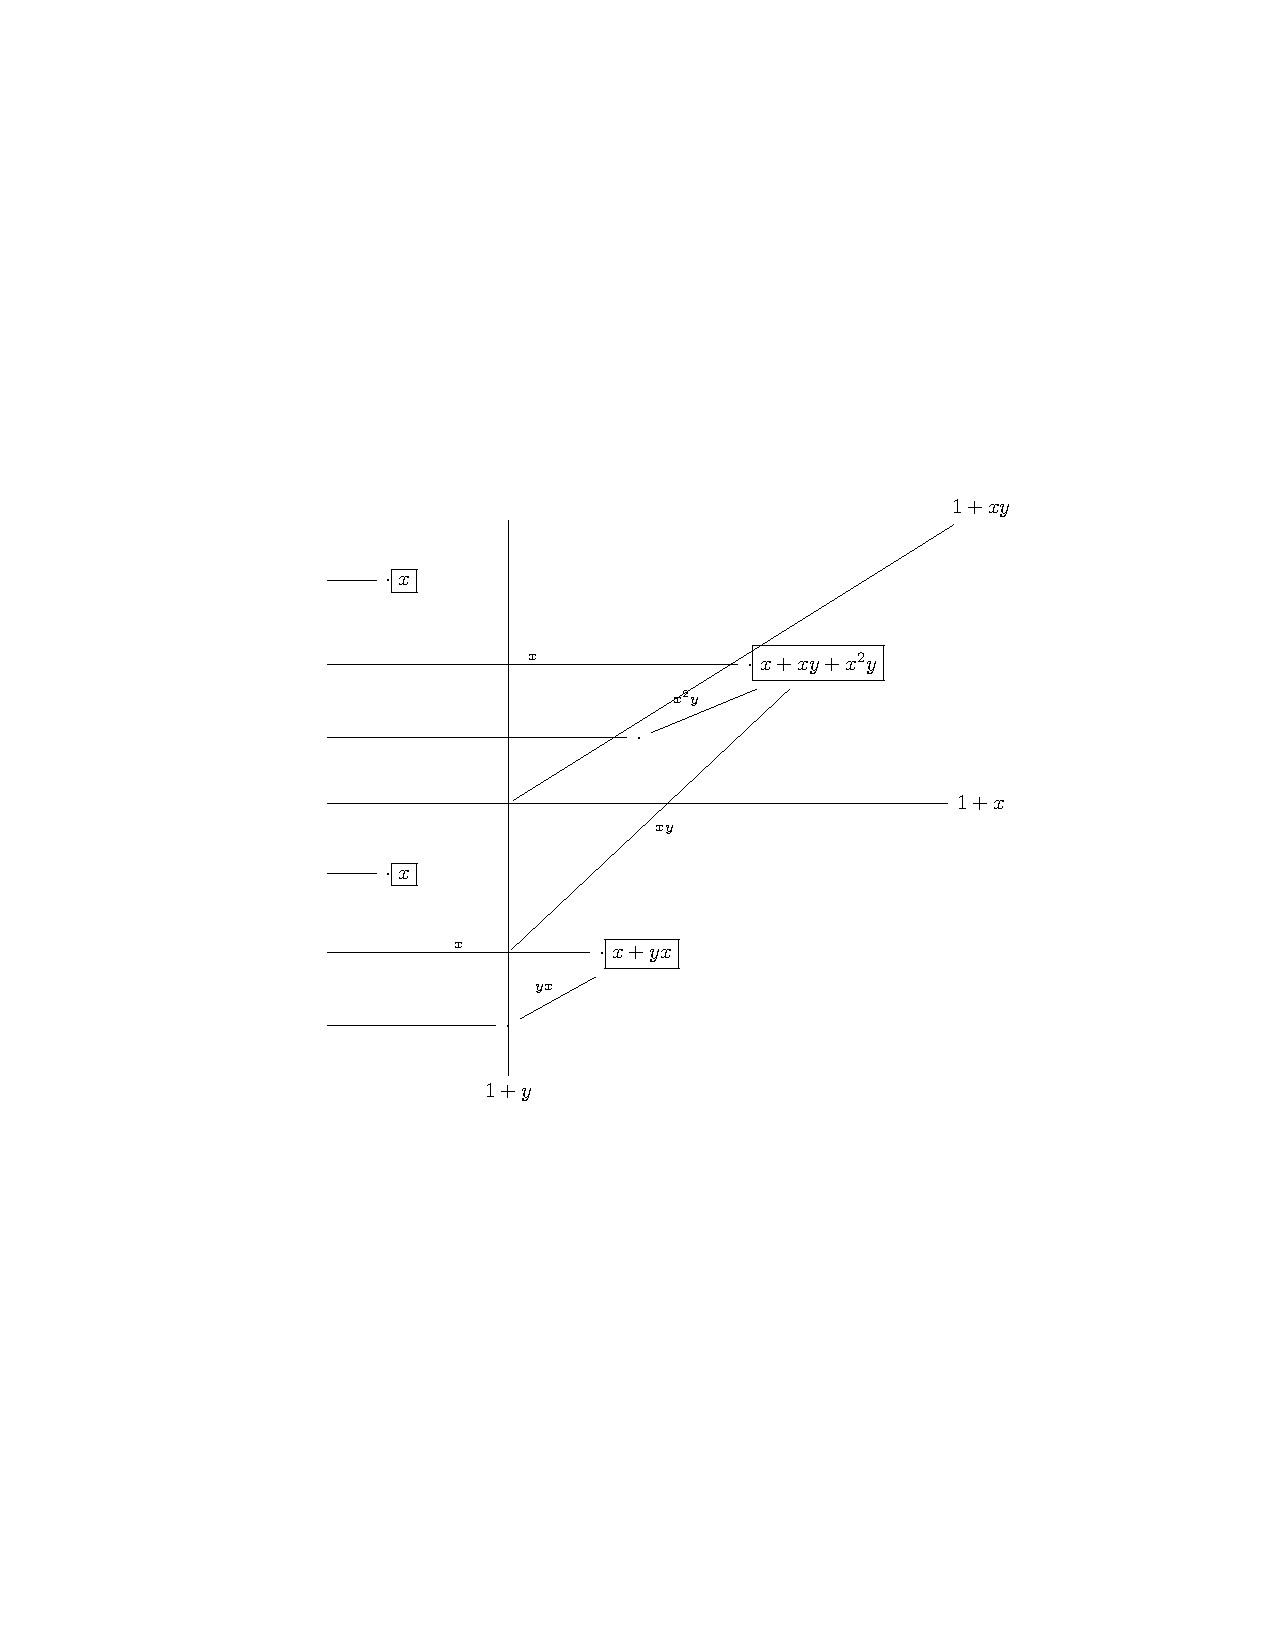
\includegraphics[width=0.8384\linewidth]{images/diagram-5-71.pdf}}}.}
\end{example}
\subsection{典范函数：广义\texorpdfstring{$\theta$}{θ}函数}
设 $\mathscr S$ 在余维不超过二处相容，$m$ 为一个渐近整向量场。用同样的构造，对折线求和得到
\Eq{5.72}{\vartheta_m\in\OO(\mathcal X^\circ).}
在 $\mathfrak u\subseteq\sigma$ 对应的 $R_{\mathfrak u}=A[\Lambda_\sigma]$ 上，定义
\Eq{5.73}{\vartheta_m=\sum_{\substack{\beta\text{ 的渐近单项式为 }z^m\\\text{终点为 }p}}b_\beta z^{m_\beta}.}
此表达式与同一腔室内的点 $p$ 的选择无关。
\subsection{构造\texorpdfstring{$\mathcal X\to\Spec A$}{X→Spec A}}
\SourcePage{93}
\thmnum{theorem}{7}\begin{theorem}\label{thm:5.7}
若 $\mathscr S$ 为 $(B,\mathscr P,\varphi)$ 上的相容壁结构，则存在部分完备化 $\mathcal X\supset\mathcal X^\circ$，满足
\Eq{5.74}{X_0=\bigcup_{\sigma\in\mathscr P}P(\sigma).}
\end{theorem}
\begin{proof}
在这里考虑的仿射情形，所有胞腔都是锥，因而没有正维有界胞腔，此时
\Eq{5.75}{\mathcal X=\Spec\left(\bigoplus_{m\in B(\ZZ)}A\vartheta_m\right).}
一般情形下，对 $\OO_{\mathcal X^\circ}(-1)$ 的总空间应用仿射构造。这里使用了如下事实：若 $X$ 为射影簇，$L\to X$ 为 $\OO_X(-1)$ 的总空间，则
\Eq{5.76}{\bigoplus_{d\ge0}\Gamma(X,\OO_X(d))\simeq\Gamma(L,\OO_L).}
在 $B$ 的层面上，这相当于在 $B$ 上方取截断锥。
\end{proof}
\subsection{构造相容壁结构}
第一种方法见文献~\cite{ref16}。在顶点附近，$B$ 有仿射坐标图，因为 $\Delta\cap|\mathscr P[0]|=\varnothing$。此时 $\mathcal X$ 是 $\mathcal Y\to\check S$ 的镜像，而 $Y_0$ 为环面簇的并。这是一个通过\Term{sanshe}{散射}进行的归纳构造，需要初始数据 $f_{\rho,v}=f_\rho$ 在余维二处满足“局部刚性”。

第二种方法见文献~\cite{ref14}，它把散射解释为环面曲面上的相对 Gromov–Witten 理论。此时 $\mathcal X$ 是对数 Calabi–Yau 曲面对 $(Y,D)$ 的镜像，$\mathcal Y\to\check S$ 且 $\dim Y_0=2$。这导向了文献~\cite{ref13} 的结果，因此可看作一种混合方法。

在即将开展的工作中，将利用 $(Y,D)$ 或 $(\mathcal Y,Y_0)$ 上的对数 Gromov–Witten 理论，其中 $\mathcal Y$ 是全纯曲线的热带化之并。
\section{内蕴镜像映射}
此处插入 Siebert 教授几周前在几何研讨班上的报告。关键是通过带穿孔的 Gromov–Witten 理论，构造与 $(Y,D)$ 或 $\mathcal Y$ 镜像的齐次坐标环。这是允许负接触阶的对数 Gromov–Witten 不变量，构造无需显式使用壁结构。由此，可以完全控制镜像构造：通过 $X$ 上的对数 Gromov–Witten 理论，从 $(X,D)$ 得到 $\mathcal Y\to S'$；或者通过退化族 $\mathcal X\to S$ 的同类理论得到 $\mathcal Y\to S'$。这实际上是亏格零的闭弦理论。

在仿射情形，先取一对 $(Y,D)$，其中 $D=\bigcup_iD_i\subset Y$ 为正规交叉除子。要求数值等价
\Eq{5.77}{K_Y+D\equiv\sum_i a_iD_i,\qquad a_i\ge0.}
这是此处对对数 Calabi–Yau 所作的全部要求。\footnote{这是一种相当宽泛的对数 Calabi–Yau 概念。}
\examnum{8}\begin{example}\label{ex:5.8}
考虑 $\PP^2$。回忆，$B(\ZZ)$ 由三个 $\NN^2$ 的副本粘合而成。对 $a,b>0$ 的 $(a,b)$，对应的接触行为为 $u\mapsto(u^a,u^b)$。环的基元素与接触阶一一对应。乘法规则为
\Eq{5.78}{\vartheta_{m_1}\vartheta_{m_2}=\sum_pN_{m_1,m_2,p}\vartheta_p,}
其中 $N_{m_1,m_2,p}$ 计数与 $D$ 的接触阶为 $m_1,m_2,-p$ 的亏格零曲线。困难之处在于证明结合律。
\end{example}
\SourcePage{94}
对固有的 Calabi–Yau 退化族，有
\Eq{5.79}{\begin{tikzcd}\mathcal Y\arrow[d]\&Y_0\arrow[l,hook]\arrow[d]\\S\&\{0\}\arrow[l,hook],\end{tikzcd}}
然后有
\Eq{5.80}{\mathcal X=\operatorname{Proj}\left(\bigoplus_m A\vartheta_m\right).}
\Lecture{26}{2019年12月3日}
面临的挑战如下：
\begin{itemize}
\item 提取 Hodge 结构变分以及亏格零的闭 Gromov–Witten 不变量；
\item 同调镜像对称（HMS）；
\item 其他镜像现象，其中还有大量开放问题：
\begin{itemize}
\item $g>0$ 的情形：非交换结构、幻影可积性；
\item 超 Kähler 情形：AAB 膜与几何 Langlands 理论；
\item Donaldson–Thomas 理论。
\end{itemize}
\end{itemize}

\chapter{同调镜像对称初探}
\SourcePage{95}
这里的内容比简单地说“导出范畴就是 Fukaya 范畴”更微妙。以下始终设 $(X,\omega)$ 为紧 Calabi–Yau 流形。
\section{概览}
此前讨论的是闭弦，图像如图~\ref{fig:6.1} 所示。拓扑扭曲产生 A 模型，即 Gromov–Witten 理论（GW），以及 B 模型，即 Hodge 结构变分（VHS）。同调镜像对称则是开弦的版本，其图像如图~\ref{fig:6.2} 所示。
\OriginalFigure{fig-6-1.pdf}{0.2946}{一条闭弦随时间传播，并分裂成两条弦。}{fig:6.1}
\OriginalFigure{fig-6-2.pdf}{0.4200}{一条开弦随时间传播，边界条件为 $L_0,L_1$。}{fig:6.2}
\SourcePage{96}
\OriginalFigure{fig-6-3.pdf}{0.3746}{圆盘到流形的映射 $u:\Delta\to X$，其边界各段映到 Lagrange 子流形 $L_i$；可把它看作一条开弦的产生与消亡。}{fig:6.3}
\OriginalFigure{fig-6-4.pdf}{0.3081}{映射 $u:\Delta\to X$ 有三个边界标记点，各段边界分别映到三个 Lagrange 子流形。计数这样的映射，将在子流形的交点集合上给出代数结构。}{fig:6.4}
于是，我们有一些满足边界条件 $L_1,L_2$ 的开弦在空间中传播。扭曲后得到 A 模型，在亏格零时由 Fukaya 范畴 $\mathcal F(X)$ 给出。\footnote{还没有人敢于在高亏格情形中作出这一定义。}B 模型由导出范畴 $D^b(\OO_X)$ 给出。
\subsection{A 模型与 B 模型}
从图像上看，弦像图~\ref{fig:6.3} 那样产生和消亡。这给出交点之间的某种量子修正。一般情形则是图~\ref{fig:6.4} 那样的多边形。

边界条件给出“对象”的集合 $\Obj(\mathcal A)$，边界条件的交点给出“态射”的集合 $\Hom(\mathcal A)$。弦的传播由态射的复合运算 $m_k$ 给出，图~\ref{fig:6.3}、\ref{fig:6.4} 为这些 $m_k$ 赋予代数结构。

设 $(X,\omega)$ 为复维数 $d$ 的辛流形。当 $\mathcal A=\mathcal F(X)$ 时，对象是\Term{lagrangeziliuxing}{Lagrange 子流形}，即满足 $\dim_{\RR} L=d$、$\omega|_L=0$ 的子流形 $L\subset X$。传播中的弦对应于映射 $u:\Delta\to X$，其中 $\Delta=\{|z|\le1\}\subset\CC$ 为闭单位圆盘。若 $L,L'$ 横截相交，则
\Eq{6.1}{\operatorname{hom}(L,L')=\CC^{L\cap L'}.}
\SourcePage{97}
\OriginalFigure{fig-6-5.pdf}{0.3443}{定义 $m_k$ 时所计数的圆盘类型。}{fig:6.5}
实际上，还希望在这些 Lagrange 子流形上配备 $U(1)$ 局部系统；交点处的系数不再只是 $\CC$，而来自对应纤维之间的同态。运算
\Eq{6.2}{m_k:\Hom(L_{k-1},L_k)\otimes\cdots\otimes\Hom(L_0,L_1)\longrightarrow\Hom(L_0,L_k)}
由计数图~\ref{fig:6.5} 中的映射 $u:\Delta\to X$ 给出，且 $u(\partial\Delta)\subset L_0\cup\cdots\cup L_k$。

B 模型中使用范畴 $D^b(\OO_X)$，即凝聚层的有界导出范畴。其对象由复形
\Eq{6.3}{F^\bullet=(\cdots\longrightarrow F^{-r}\longrightarrow F^{-r+1}\longrightarrow\cdots)}
表示，要求上同调有界：\footnote{上标 $b$ 就表示有界。}
\Eq{6.4}{h^i(F^\bullet)=0\qquad\text{当 }|i|\gg0.}
这为什么重要？闭弦的故事主要是计数几何，关注它的人相对有限；开弦的故事则带来许多人关心的新对象。Lagrange 子流形是辛几何的重要目标，而导出范畴在几何表示论、代数几何等领域都非常重要。
\subsection{代数结构}
定义域的模空间，即稳定圆盘的模空间，具有递归结构。
\examnum{1}\begin{example}\label{ex:6.1}
考虑边界上有四个标记点的圆盘。计数其上的映射给出 $m_3$。它能以多种方式退化，其中两种见图~\ref{fig:6.6}。把标记点 $0$ 看作输出，其余点看作输入。这些退化可用带根的度量带状树编码，\footnote{带状图是指每个顶点处的边带有循环次序的图。这里的带状树总可嵌入平面。}对应的树也画在图~\ref{fig:6.6} 中。
\end{example}
对于两两横截的 $L_0,\ldots,L_k$，可通过对圆盘到 $X$ 的 $J$ 全纯映射作虚拟计数，定义
\Eq{6.5}{m_k:\Hom(L_{k-1},L_k)\otimes\cdots\otimes\Hom(L_0,L_1)\longrightarrow\Hom(L_0,L_k)[2-k].}
此模空间的虚拟维数为
\Eq{6.6}{(k-2)+d_0-\sum_{i=1}^kd_i.}
\SourcePage{98}
\OriginalFigure{fig-6-6.pdf}{0.8056}{四标记点圆盘的两种退化，以及相应的带根带状树。}{fig:6.6}
在适当条件下，交点带有 $\ZZ$ 分次，这就是移位 $[2-k]$ 的含义。研究高维模空间的边界，便得到 $m_k$ 之间的代数关系。
\examnum{2}\begin{example}\label{ex:6.2}
\begin{enumerate}[label=(\alph*)]
\item 第一个关系为 $m_1^2=0$，即 $m_1$ 是微分。取两个 Lagrange 子流形 $L_0,L_1$；令交点次数差为 $2$，便可看到条带断裂的边界，从而说明 $m_1$ 是
\Eq{6.7}{\bigoplus_{L,L',d}\Hom^d(L,L')}
上的微分。
\item 有关系
\Eq{6.8}{m_1m_2=m_2(m_1\otimes\id+\id\otimes m_1),}
它表达了 $m_1$ 相对于 $m_2$ 的分次 Leibniz 法则。
\item $m_2$ 本身未必结合，$m_3$ 则提供结合性的同伦。具体地，
\Eq{6.9}{\begin{aligned}m_2(\id\otimes m_2-m_2\otimes\id)={}&m_1m_3\\&+m_3(m_1\otimes\id\otimes\id+\id\otimes m_1\otimes\id+\id\otimes\id\otimes m_1).\end{aligned}}
右侧第一项是上边缘，第二项在 $m_1$-上闭链上为零。
\item 一般公式为
\Eq{6.10}{\sum_{\substack{p\ge1,\ q\ge0\\p+q\le k}}(-1)^{|a_1|+\cdots+|a_q|-q}\,m_{k-p+1}(a_k,\ldots,a_{p+q+1},m_p(a_{p+q},\ldots,a_{q+1}),a_q,\ldots,a_1)=0.}
\end{enumerate}
这些称为 $A_\infty$ 关系。
\end{example}
\SourcePage{99}
\subsection{Fukaya 范畴}
假定 $c_1(X)=0$，$X$ 紧，所有 $L_i$ 均定向、带有自旋结构与分次，并且无障碍。\footnote{例如，不存在以 $L_i$ 为边界的非恒值全纯圆盘时，这一条件成立。}此时可对两两横截的 Lagrange 子流形 $L_0,\ldots,L_k$ 定义 $m_k$。自然的系数环是 Novikov 环：
\Eq{6.11}{\Lambda_{\mathrm{nov}}=\left\{\sum_{i\ge0}a_iq^{\lambda_i}:\lambda_i\in\RR,\ \lambda_i\to+\infty,\ a_i\in\ZZ\right\}.}
也可以取 $a_i\in\QQ$ 或 $\CC$，此时得到\Term{novikovyu}{Novikov 域}。$a_i$ 来自全纯圆盘的计数，而 $\lambda_i$ 是相应圆盘的辛面积：
\Eq{6.12}{\int_\Delta u^*\omega.}
先验而言，这只给出 $A_\infty$ 预范畴，因为 $\Hom(L,L)$ 在横截交点的定义下没有意义。可用 Hamilton 扰动解决这一问题：对 $L,L'$，选取 $H_t:X\to\RR$，$t\in[0,1]$，其 Hamilton 流 $\varphi_t$ 满足 $\varphi_1(L')\pitchfork L$。可以证明，所得 $A_\infty$ 范畴 $\mathcal F(X)$ 在典范的 $A_\infty$ 拟等价意义下良定义。现在正式给出定义。
\thmnum{definition}{1}\begin{definition}\label{def:6.1}
一个非幺 $A_\infty$ 代数，是 $\ZZ$ 分次 $K$ 向量空间
\Eq{6.13}{A=\bigoplus_{p\in\ZZ}A^p,}
连同对每个 $k\ge1$ 的次数零分次 $K$ 线性映射
\Eq{6.14}{m_k:A^{\otimes k}\longrightarrow A[2-k],}
它们满足 $A_\infty$ 关系。
\end{definition}
\thmnum{definition}{2}\begin{definition}\label{def:6.2}
一个非幺 $A_\infty$ 范畴 $\mathcal A$，由对象集合 $\Obj(\mathcal A)$，对每对对象 $X_0,X_1$ 的 $\ZZ$ 分次 $K$ 向量空间
\Eq{6.15}{\Hom(X_0,X_1),}
以及对每个 $k\ge1$ 的映射
\Eq{6.16}{m_k:\Hom(X_{k-1},X_k)\otimes\cdots\otimes\Hom(X_0,X_1)\longrightarrow\Hom(X_0,X_k)[2-k]}
组成，且满足 $A_\infty$ 关系。
\end{definition}
对 $A_\infty$ 范畴取其上同调范畴 $H(\mathcal F(X))$，就得到通常的范畴：对象不变，态射空间取关于 $m_1$ 的上同调；此时 $m_1=0$。
\begin{custom}{事实 9}\hypertarget{fact:9}{}$H(\mathcal F(X))$ 是幺范畴，即对每个 $L$，都存在某个 $e_L\in\Hom^0(L,L)$，满足 $m_1(e_L)=0$，它对 $m_2$ 起单位元作用，而以它为输入时，所有 $k>2$ 的 $m_k$ 均为零。\end{custom}
这样的范畴称为上同调幺范畴，或 $c$ 幺范畴。它稍有不便，不过有一种技巧：$c$ 幺范畴 $\mathcal F(X)$ 可以证明与某个严格幺 $A_\infty$ 范畴 $A_\infty$-拟等价。
\SourcePage{100}
\subsection{“导出”Fukaya 范畴}
这里也许会产生疑问：如何把这个 $A_\infty$ 范畴与一个三角导出范畴对应？Kontsevich 的办法是人为加入复形，把 $\mathcal A=\mathcal F(X)$ 扩张为一个“三角 $A_\infty$ 范畴” $\operatorname{Tw}\mathcal F(X)$。
具体地，对 $L_1,\ldots,L_k$，取 $\Delta=(\delta_{ij})$，$\delta_{ij}\in\Hom^1(L_j,L_i)$，满足：
\begin{itemize}
\item 严格下三角：当 $j\ge i$ 时 $\delta_{ij}=0$；
\item Maurer–Cartan 方程：
\Eq{6.17}{\sum_{r\ge1}m_r(\Delta,\ldots,\Delta)=\sum_{\substack{i_0<\cdots<i_r\\r\ge1}}m_r(\delta_{i_r,i_{r-1}},\ldots,\delta_{i_1,i_0})=0.}
\end{itemize}
\Lecture{27}{2019年12月5日}
\subsection{同调镜像对称}
现在给出同调镜像对称的精确陈述。回忆，Fukaya 范畴的系数属于 Novikov 域；采用复系数，令 $K=\Lambda_{\mathrm{nov},\CC}$。紧 Calabi–Yau 流形 $(X,\omega)$ 给出镜像的极大退化族 $Y/S$，此处在 $S=\Spec K$ 上工作。
\begin{custom}{猜想 1}\hypertarget{conj:1}{}
在 $K$ 上，存在典范的 $A_\infty$ 范畴等价
\Eq{6.18}{\psi:D^b\mathcal F(X)=H^0(\operatorname{Tw}^{\Pi}\mathcal F(X))\xrightarrow{\sim}D^b(Y).}
\end{custom}
$\operatorname{Tw}^{\Pi}\mathcal F(X)$ 称为分裂闭包；换言之，它是在扭曲 Fukaya 范畴中加入幂等元的像所得到的完备化。
\section{导出范畴的微分分次增强与同调扰动引理}
\subsection{导出范畴的\texorpdfstring{Čech}{Čech}模型}
微分分次范畴，即 dg 范畴，是 $k>2$ 时 $m_k=0$ 的 $A_\infty$ 范畴。我们希望描述 $D^b(X)$ 的 $A_\infty$ 结构。关键在于，取上同调后仍可保留一个 $A_\infty$ 结构。\Term{tongdiaoraodongyinli}{同调扰动引理}（HPL）说明：即使从 dg 范畴出发，传到上同调后的结构一般也只是 $A_\infty$ 的。

假定 $X$ 光滑且射影。每个凝聚 $\OO_X$ 模都有有限的局部自由消解，故
\Eq{6.19}{D^b(X)=D^b(\operatorname{Coh}X)=\operatorname{Perf}(X).}
一般而言，拟凝聚层导出范畴中的完美复形就是紧对象；不过若从一开始就假定射影，所涉及的对象本来就都是紧的。

dg 增强如下：$D^b_{\mathrm{dg}}(X)$ 的对象是局部自由层的有界复形，态射才是需要说明的部分。记 $X$ 的有限仿射覆盖为
\Eq{6.20}{\mathscr U=\{U_i\}.}
令
\Eq{6.21}{\Hom(E^\bullet,F^\bullet)=\bigoplus_n\Hom^n_{D^b_{\mathrm{dg}}(X)}(E^\bullet,F^\bullet),}
其中
\Eq{6.22}{\Hom^n_{D^b_{\mathrm{dg}}(X)}(E^\bullet,F^\bullet)=\bigoplus_{p+q=n}\check C^p(\mathscr U,\mathcal Hom^q_{\OO_X}(E^\bullet,F^\bullet)).}
这里记
\Eq{6.23}{\mathcal Hom_{\OO_X}(E^\bullet,F^\bullet[q])=\mathcal Hom^q_{\OO_X}(E^\bullet,F^\bullet),}
\SourcePage{101}
$\check C^p$ 为 Čech $p$ 上链：
\Eq{6.24}{\check C^p(\mathscr U,\mathcal G)=\bigoplus_{i_0<\cdots<i_p}\Gamma(U_{i_0}\cap\cdots\cap U_{i_p},\mathcal G).}
这构成 dg 范畴，微分 $m_1$ 由 Čech 微分和内部 Hom 微分给出。
对于
\Eq{6.25}{f=(f_{n,i_0,\ldots,i_p})\in\check C^p(\mathscr U,\mathcal Hom^q(E^\bullet,F^\bullet)),}
\Eq{6.26}{g=(g_{n',i_0,\ldots,i_{p'}})\in\check C^{p'}(\mathscr U,\mathcal Hom^{q'}(F^\bullet,G^\bullet)),}
复合为
\Eq{6.27}{m_2(g,f)=(-1)^{\deg f}g\circ f,}
其中
\Eq{6.28}{g\circ f=\left((-1)^{q'p}g_{n+q,i_0,\ldots,i_{p'}}\circ f_{n,i_{p'},\ldots,i_{p+p'}}\right)\big|_{U_{i_0}\cap\cdots\cap U_{i_{p+p'}}}.}
\subsection{同调扰动引理}
\thmnum{theorem}{1}\begin{theorem}\label{thm:6.1}
对任意定义在域上的 $A_\infty$ 范畴 $\mathcal A$，其上同调 $H(\mathcal A)$ 上存在 $m_1=0$ 的 $A_\infty$ 范畴结构，称为极小 $A_\infty$ 范畴，并且有 $A_\infty$ 拟等价 $H(\mathcal A)\to\mathcal A$。
\end{theorem}
\begin{proof}
该构造依赖于对每对对象 $X,Y$ 选择投影算子 $\Pi$ 与同伦 $H$：
\Eq{6.29}{\Pi:\Hom(X,Y)\longrightarrow\Hom(X,Y),}
\Eq{6.30}{H:\Hom(X,Y)\longrightarrow\Hom(X,Y)[-1],}
其中 $\Pi$ 次数为零，$\Pi^2=\Pi$，并满足
\Eq{6.31}{\Pi-\id=m_1H+Hm_1.}
这将给出所需的拟等价。取 $\Pi$ 为到上同调类的闭代表元所组成子空间的投影。

得到一个新 $A_\infty$ 范畴 $\Pi\mathcal A$，其对象不变，态射为
\Eq{6.32}{\Hom_{\Pi\mathcal A}(X,Y)=\Pi(\Hom_{\mathcal A}(X,Y))\subset\Hom_{\mathcal A}(X,Y),}
故 $H(\Pi\mathcal A)=H(\mathcal A)$。定义运算如下：
\Eq{6.33}{m_1^\Pi=m_1,}
\Eq{6.34}{m_2^\Pi=\Pi\circ m_2,}
\Eq{6.35}{m_k^\Pi=\sum_{\substack{T\text{ 为带根带状树}\\T\text{ 有 }k\text{ 个叶子}}}m_{k,T}\qquad(k\ge3).}
这些规则可看作 Feynman 规则：每个有 $r+1$ 条邻接边的内部顶点放置 $m_r$，内部边放置 $H\circ$，根端放置 $\Pi\circ$。
\examnum{3}\begin{example}\label{ex:6.3}
取 $k=6$。图~\ref{fig:6.7} 给出求和中的一棵带根带状树，其贡献为
\Eq{6.36}{m_{6,T}(a_1,\ldots,a_6)=\Pi m_3(a_1,Hm_2(Hm_3(a_2,a_3,a_4),a_5),a_6).}
\end{example}
\SourcePage{102}
\OriginalFigure{fig-6-7.pdf}{0.5328}{对 $m_6^\Pi$ 的定义作出贡献的一棵带根带状树。}{fig:6.7}
\thmnum{lemma}{2}\begin{lemma}\label{lem:6.2}
$m_k^\Pi$ 满足 $A_\infty$ 关系。
\end{lemma}
\begin{Note}{6.1}存在 $A_\infty$ 函子
\Eq{6.37}{(i_k):\Pi\mathcal A\longrightarrow\mathcal A,}
它与 $H(\mathcal A)$ 上由 $m_k^\Pi$ 给出的 $A_\infty$ 结构相容。$i_1$ 为包含映射；其余 $i_k$ 用类似的树构造定义：
\Eq{6.38}{i_k=\sum_{\substack{T\text{ 为带根带状树}\\T\text{ 有 }k\text{ 个叶子}}}i_{k,T}\qquad(k\ge2),}
其中 $i_{k,T}$ 与 $m_{k,T}$ 的定义相同，只把根端的 $\Pi$ 换成 $H$。
\end{Note}
\thmnum{lemma}{3}\begin{lemma}\label{lem:6.3}
$(i_k)$ 是 $A_\infty$ 函子。
\end{lemma}
\end{proof}
\begin{proof}[引理~\ref{lem:6.2} 的证明概要]
考虑
\Eq{6.39}{\mu_k=\sum_{\substack{T\text{ 为带状树}\\e\text{ 为一条边}}}\mu_{k,(T,e)}.}
其中 $\mu_{k,(T,e)}$ 与 $m_{k,T}$ 的构造相同，但在内部边 $e$ 上，把 $H$ 换成 $\Pi-\id=m_1H+Hm_1$；对于外部边，则放置 $m_1$。有两种整理方式：
\begin{enumerate}[label=(\roman*)]
\item 使用 $\Pi-\id$，按边 $e$ 分类：
\Eq{6.40}{\mu_k=\underbrace{\mu_k^{m_1}}_{e\text{ 为外部边}}+\underbrace{\mu_k^\Pi-\mu_k^{\id}}_{e\text{ 为内部边}}.}
\item 使用 $m_1H+Hm_1$，按与 $e$ 相邻的内部顶点分类。
\end{enumerate}
再对各 $m_r$ 应用 $A_\infty$ 关系，得到新的树求和，其中每项出现在 $\mu_k^{\id}$ 中。核对分次符号后，$\mu_k=-\mu_k^{\id}$。由\eqref{eq:6.40}得
\Eq{6.41}{\mu_k^{m_1}+\mu_k^\Pi=0.}
这恰好是 $m_k^\Pi$ 的 $A_\infty$ 关系。
\end{proof}
\SourcePage{103}
\section{Polishchuk 的刚性定理}
\subsection{约化到代数\texorpdfstring{$A_L$}{AL}}
先设 $X$ 为光滑射影簇，$L\in D^b(X)$ 为丰线丛。在 $D^b_{\mathrm{dg}}(X)$ 中，取以 $L^n$（$n\in\ZZ$）为对象的全子范畴 $\langle L\rangle$。在 $D^b(X)=H(D^b_{\mathrm{dg}}(X))$ 上，$m_2$ 由下列代数上的杯积给出：
\Eq{6.42}{A_L=\bigoplus_{p,q\in\ZZ}H^p(X,L^q).}
注意，$A_L$ 包含齐次坐标环：
\Eq{6.43}{A_L\supseteq R_L=\bigoplus_{n\ge0}H^0(X,L^n).}
$A_L$ 带有极小\footnote{这表示 $m_1=0$。}$A_\infty$ 代数结构，而 $\langle L\rangle$ 分裂生成 $D^b(X)$。因此，$A_L$ 连同其内部幂次分次及 $A_\infty$ 代数结构，刻画了 $D^b(X)$ 的 $A_\infty$ 范畴结构。
\Lecture{28}{2019年12月10日}
\subsection{\texorpdfstring{$A_L$ 上的 $A_\infty$ 结构}{AL 上的 A∞ 结构}}
于是有如下问题。
\setcounter{prob}{0}\begingroup\renewcommand{\theprob}{\arabic{prob}}\begin{problem}\label{problem:6.1}
除 $m_2$ 之外，$A_L$ 上的 $A_\infty$ 结构还保存了多少信息？
\end{problem}\endgroup
\begin{Note}{6.2}
设 $X$ 为特征零域上的 $d$ 维光滑射影 Calabi--Yau 簇，且 $H^p(X,\OO_X)=0$ 对 $0<p<d$ 成立，则有
\Eq{6.44}{\begin{aligned}
A_L&=\bigoplus_{p\ge0,\ q\in\ZZ}H^p(X,L^{\otimes q})\\
&=\bigoplus_{q\ge0}H^0(X,L^{\otimes q})
\oplus\bigoplus_{q\le0}\underbrace{H^d(X,L^{\otimes q})}_{\simeq H^0(X,L^{\otimes(-q)})^*}.
\end{aligned}}
\end{Note}
\begin{Note}{6.3}线丛 $L$ 的幂次给出了一个内部次数分次。\end{Note}
\thmnum{theorem}{4}\begin{theorem}[Polishchuk]\label{thm:6.4}
设 $X$ 为 $d$ 维射影簇，$d\ge1$，$L$ 为甚丰线丛，并且对所有 $p\in\ZZ$ 及 $q\ne0,d$，都有 $H^q(X,L^{\otimes p})=0$。则：
\begin{enumerate}[label=(\roman*)]
\item 在严格 $A_\infty$ 同构（这里指 $(f_n)$ 满足 $f_1=\id$）与缩放的意义下，$A_L$ 上存在唯一的保持内部次数、扩张既定 $m_2$ 的非平凡极小 $A_\infty$ 结构。非平凡表示它不能通过这样的同构化为所有 $k>2$ 的 $m_k$ 均为零的结构。
\item 两个给定结构之间的严格 $A_\infty$ 同构，在同伦意义下唯一。
\end{enumerate}
\end{theorem}
\begin{Note}{6.4}
这说明，同调镜像对称的内容在某种意义下可以集中到一个很小的部分。刚性的作用在于：要证明同调镜像对称，只需把两边的环对应起来，再验证这少量额外的信息一致。
\end{Note}
\subsection{\texorpdfstring{$A_\infty$}{A∞}结构与 Hochschild 上闭链}
设 $A=\bigoplus_{k\in\ZZ}A^k$ 为分次代数，$(m_n)$ 与 $(m'_n)$ 是其两个 $A_\infty$ 扩张，其中 $m_1=m'_1=0$，$m_2=m'_2$ 为给定的乘法。如果对所有 $i<n$，都有 $m_i=m'_i$，那么：
\begin{enumerate}[label=(\roman*)]
\item $c=m_n-m'_n$ 是一个 Hochschild $n$ 上闭链，其上边缘算子为
\Eq{6.45}{\begin{aligned}
\delta c(a_1,\ldots,a_{n+1})={}&(-1)^{n\deg a_1}a_1c(a_2,\ldots,a_{n+1})\\
&+\sum_{j=1}^{n}(-1)^j c(a_1,\ldots,a_ja_{j+1},\ldots,a_{n+1})\\
&+(-1)^{n+1}c(a_1,\ldots,a_n)a_{n+1}.
\end{aligned}}
这是因为，把两个 $A_\infty$ 关系相减后，只剩下这些项。
\item 用保持较低阶数据的严格 $A_\infty$ 同构改变 $m_n$，只会给 $c$ 加上一个 Hochschild 上边缘。
\end{enumerate}
\SourcePage{104}
\subsection{这里的具体情形}
现在 $A=R\oplus M$，其中
\Eq{6.46}{R=\bigoplus_{q\ge0}H^0(X,L^q),\qquad\deg R=0,}
\Eq{6.47}{M=\bigoplus_{q\le0}H^d(X,L^q),\qquad\deg M=d,}
且
\Eq{6.48}{m_n:A^{\otimes n}\longrightarrow A[2-n].}
考察次数。如果输入 $a_i$ 中有 $k$ 个属于 $M$，则输入总次数为 $kd$，其中 $0\le k\le n$，输出次数为 $kd+2-n$。由于 $A$ 只有次数 $0$ 与 $d$，必有
\Eq{6.49}{kd+2-n=0\qquad\text{或}\qquad(k-1)d+2-n=0.}
因此，令 $l=k$ 或 $k-1$，则在非零的情形中 $n=ld+2$，$0\le l\le n$。两个结构第一次不同之处，$c=m_n-m'_n$ 是内部次数零、上同调次数 $2-n$ 的 Hochschild 上闭链，记作
\Eq{6.50}{c\in C^n_{0,n-2}=C^{ld+2}_{0,ld}.}
下标依次记录内部次数与上同调次数的相反数。
\subsection{标准 bar 消解、cobar 复形与 Hochschild 上同调}
设 $A$ 为结合 $k$ 代数，其中 $k$ 是交换幺环，并给定满的增广映射 $\epsilon:A\twoheadrightarrow k=A/A_+$。考虑复形
\Eq{6.51}{\cdots\longrightarrow A_+\otimes A_+\otimes A
\longrightarrow A_+\otimes A\longrightarrow A\xrightarrow{\epsilon}k\longrightarrow0.}
取 $a_1,\ldots,a_n\in A_+$，$a_{n+1}\in A$，其微分由相邻因子的乘法给出：
\Eq{6.52}{d(a_1\otimes\cdots\otimes a_{n+1})=
\sum_{i=1}^{n}(-1)^i a_1\otimes\cdots\otimes a_ia_{i+1}\otimes\cdots\otimes a_{n+1}.}
\begin{custom}{事实 10}\hypertarget{fact:10}{}这是一个复形，即 $d^2=0$。\end{custom}
当 $A$ 有单位元时，此增广复形正合。这称为 \Term{bargouzao}{bar 构造}。\footnote{Eilenberg 与 Mac Lane 最初写出这一构造时，用竖线 $|$ 简记张量积；名称 bar 正由此而来。}
对 $A$ 双模 $M$，令
\Eq{6.53}{C^n(A,M):=\Hom_k(A_+^{\otimes n},M).}
它与上边缘算子 $\delta$ 构成复形，称为 cobar 复形。其上同调为
\Eq{6.54}{HH^n(A,M):=H^n(C^\bullet(A,M),\delta),}
\Eq{6.55}{HH^n(A):=HH^n(A,A),}
称为 \Term{Hochschildshangtongdiao}{Hochschild 上同调}。内部次数与上同调次数给出两重分次，例如记为
\Eq{6.56}{HH^n_{0,n-2}(A).}
\begin{Note}{6.5}一般的 $A_\infty$ 代数也有 Hochschild 同调与上同调，不过这里不需要使用它们。\end{Note}
\SourcePage{105}
\subsection{刚性定理的证明}
\thmnum{proposition}{5}\begin{proposition}\label{prop:6.5}
对上述 $A=R\oplus M$，有：
\begin{enumerate}[label=(\roman*)]
\item 对所有 $l\ge1$ 及 $i<l(d+2)$，
\Eq{6.57}{HH^i_{0,ld}(A)=0.}
\item $\dim HH^{d+2}_{0,d}(A)\le1$。
\end{enumerate}
\end{proposition}
\thmnum{corollary}{6}\begin{corollary}\label{cor:6.6}
两个 $A_\infty$ 扩张 $(m_n)$ 与 $(m'_n)$ 严格 $A_\infty$ 同构，当且仅当
\Eq{6.58}{[m_{d+2}-m'_{d+2}]=0\in HH^{d+2}_{0,d}(A).}
\end{corollary}
\begin{proof}
逐阶比较并消去差异。在当前第一次不同的阶数，有 $[m'_n-m_n]\in HH^{ld+2}_{0,ld}(A)$，其中 $0\le l\le n$。当 $l>1$ 时，$ld+2<l(d+2)$，故由命题~\ref{prop:6.5}，这个类自动为零。对于 $n>2$，只需另行考察 $l=1$，也就是 $m'_{d+2}-m_{d+2}$。
\end{proof}
\begin{proof}[定理~\ref{thm:6.4} 的证明]
由命题~\ref{prop:6.5} 的第(ii)项与推论~\ref{cor:6.6}，或者所有高阶运算都能消去，或者非平凡结构在缩放意义下唯一。
\end{proof}
\begin{Note}{6.6}
对光滑 $X$ 的典范结构，$[m_{d+2}]\ne0$，所以出现的是第二种可能。其依据是考察一点的理想层并取 Koszul 消解，从而得到 $m_{d+2}\ne0$。
\end{Note}
\begingroup\setstretch{1.15}
\setlength{\abovedisplayskip}{1pt}
\setlength{\belowdisplayskip}{1pt}
\setlength{\abovedisplayshortskip}{0pt}
\setlength{\belowdisplayshortskip}{1pt}
\begin{proof}[命题~\ref{prop:6.5} 的证明]
由 $A=R\oplus M=k\oplus R_+\oplus M$，对固定的 $l$，可写成
\Eq{6.59}{C^i:=C^i_{0,ld}=\underbrace{C^i(0)}_{\text{输出次数 }0}
\oplus\underbrace{C^i(d)}_{\text{输出次数 }d}.}
这些空间分别包含于
\Eq{6.60}{C^i(0)\subset\Hom(A_+^{\otimes i},R),}
\Eq{6.61}{C^i(d)\subset\Hom(A_+^{\otimes i},M).}
上链的形状如下。对 $c\in C^i(0)$，
\Eq{6.62}{c:[T(R_+)\otimes M\otimes T(R_+)\otimes\cdots\otimes M\otimes T(R_+)]_i\longrightarrow R.}
这里 $T(R_+)$ 为定义在 $k$ 上的张量代数，下标 $i$ 表示属于 $H^*(L^*)$ 的因子总数。对于 $C^i(d)$，有类似的描述。
由此得到正合序列
\Eq{6.63}{0\longrightarrow C^\bullet(d)\longrightarrow C^\bullet\longrightarrow C^\bullet(0)\longrightarrow0.}
因此，只需证明：
\begin{enumerate}[label=(\roman*)]
\item 对 $i<l(d+2)$，$H^i(C^\bullet(0))=H^i(C^\bullet(d))=0$；
\item 当 $l=1$ 时，$H^{d+2}(C^\bullet(d))=0$ 且 $\dim H^{d+2}(C^\bullet(0))\le1$。
\end{enumerate}
先按输出在 $R$ 中的内部次数分解：
\Eq{6.64}{C^\bullet(0)=\prod_{j\ge0}C^\bullet(0)_j.}
微分 $\delta$ 的形式为
\Eq{6.65}{\delta(x_j)_{j\ge0}=\left(\sum_{j\le j'}\delta_{j,j'}x_j\right)_{j'\ge0}.}
\SourcePage{106}
相邻因子相乘时，$M$ 因子的数目不会增加。现在利用下式逐步归纳：
\Eq{6.66}{0\longrightarrow\operatorname{gr}_i C^\bullet(0)
\longrightarrow}
这意味着，可以在各个 $(C^\bullet(0)_j,\delta_{j,j})$ 的上同调上验证第(i)、(ii)项。它们可写作
\Eq{6.67}{(C^\bullet(0)_j,\delta_{j,j})=\Hom(K^\bullet_{l,j},R_j)[-l],}
其中 $K^\bullet_{l,j}$ 为下述复形的第 $j$ 个内部次数分量：
\Eq{6.68}{K^\bullet_l=B^\bullet(k,M,\ldots,M,k).}
这里使用某种推广的 bar 复形：
\Eq{6.69}{B^\bullet(M_1,\ldots,M_n)
=M_1\otimes T(R_+)\otimes M_2\otimes\cdots\otimes T(R_+)\otimes M_n.}
相应的 bar 复形计算可以对 $n$ 归纳。这就是此处使用的 \href{https://arxiv.org/abs/math/0302178}{Polishchuk 的命题 3.7}。把 $B^\bullet(M_1,\ldots,M_n)$ 看成一个双复形的总复形，其双次数为
\Eq{6.70}{\deg_{0/1}(x_1\otimes t_1\otimes\cdots\otimes t_{n-1}\otimes x_n)
=\sum_{\substack{i\equiv0/1\pmod2}}\deg(t_i),}
于是谱序列的 $E_1$ 页形如
\Eq{6.71}{\begin{aligned}
H^*(M_1\otimes T(R_+)\otimes M_2)\otimes T(R_+)
\otimes H^*(M_3\otimes T(R_+)\otimes M_4)\otimes\cdots.
\end{aligned}}
接下来使用以下引理。
\thmnum{lemma}{7}\begin{lemma}\label{lem:6.7}
若 $M_1$ 与 $M_2$ 在左分次 $R$ 模和右分次 $R$ 模的意义下均同构于 $M$，则
\Eq{6.72}{H^i(B^\bullet(M_1,M_2))=
\begin{cases}M,&i=-d-1,\\0,&\text{其他情形},\end{cases}}
其中第一个同构分别是在左、右分次 $R$ 模意义下的同构。
\end{lemma}
因此，$E_1$ 在适当移位后化为 $B^\bullet(M'_1,\ldots,M'_{n'})$，其中 $n'<n$。
\end{proof}\endgroup

\backmatter
\nocite{*}
\printbibliography[heading=bibintoc,title={参考文献}]
\printindex
\end{document}
